% Analytical paper (Structure B style): what an exact solution remembers about its equation.

% ---- begin ../shared/docclass.tex
% Document class selection (\input as the first line of each main.tex).
% SIMODS is typeset with SIAM's online-journal class siamonline<date>.cls. The class is not on CTAN;
% download it from SIAM's author page (the CI tries to) and place it in paper/shared/siam/.
% Without it the paper builds with a compatible fallback (article + siamshim.tex), so that text,
% numbering and cross-references can be checked; the submission must use the official class.
\makeatletter
\let\pf@cls\relax
\IfFileExists{siamonline220329.cls}{\def\pf@cls{siamonline220329}}{}
\IfFileExists{siamonline250211.cls}{\def\pf@cls{siamonline250211}}{}
\ifx\pf@cls\relax
  \documentclass[11pt]{article}
  \def\paperclass{shim}
\else
  \edef\pf@doc{\noexpand\documentclass[review,onefignum,onetabnum]{\pf@cls}}
  \pf@doc
  \def\paperclass{siam}
\fi
\makeatother

% ---- end ../shared/docclass.tex


% ---- begin ../shared/preamble.tex
% Common preamble of both papers (after docclass.tex).
\def\pfshimname{shim}
\ifx\paperclass\pfshimname
  
% ---- begin ../shared/siamshim.tex
% Fallback that mimics the parts of siamonline used by the papers (only when the class is absent).
\usepackage[letterpaper,margin=1.15in]{geometry}
\usepackage{amsmath,amssymb,amsthm}
\usepackage[T1]{fontenc}
\usepackage{lmodern}
\usepackage{fancyhdr}
\newcommand{\headers}[2]{\pagestyle{fancy}\fancyhf{}\fancyhead[LE]{\small\thepage\quad\textsc{#2}}%
  \fancyhead[RO]{\small\textsc{#1}\quad\thepage}\fancyhead[LO,RE]{}\renewcommand{\headrulewidth}{0pt}}
\newcommand{\email}[1]{\texttt{#1}}
\newcommand{\funding}[1]{\par\noindent\textbf{Funding:} #1}
\newenvironment{keywords}{\par\smallskip\noindent\textbf{Key words.}\ }{\par}
\newenvironment{MSCcodes}{\par\smallskip\noindent\textbf{MSC codes.}\ }{\par}
\newenvironment{AMS}{\par\smallskip\noindent\textbf{AMS subject classifications.}\ }{\par}
\renewenvironment{abstract}{\par\small\noindent\textbf{Abstract.}\ }{\par\normalsize}

% ---- end ../shared/siamshim.tex

\else
  \usepackage{amssymb}
  \newsiamremark{remark}{Remark}
  \newsiamremark{example}{Example}
  \newsiamthm{assumption}{Assumption}
\fi
\usepackage{mathtools}
\usepackage{graphicx}
\graphicspath{{../shared/figures/}}
\usepackage{booktabs,array,tabularx,multirow}
\usepackage[dvipsnames]{xcolor}
\usepackage{tikz}
\usetikzlibrary{arrows.meta,positioning,calc,fit,shapes.geometric,backgrounds}
\usepackage{algorithm}
\usepackage{algpseudocode}
\usepackage{enumitem}
\setlist{nosep,leftmargin=*}
\ifx\paperclass\pfshimname
  \usepackage[hidelinks]{hyperref}
  \usepackage[capitalize,nameinlink]{cleveref}
  
% ---- begin ../shared/siamshim_thm.tex
% Fallback theorem environments (loaded after hyperref and cleveref so that names resolve).
\theoremstyle{plain}
\newtheorem{theorem}{Theorem}[section]
\newtheorem{lemma}[theorem]{Lemma}
\newtheorem{proposition}[theorem]{Proposition}
\newtheorem{corollary}[theorem]{Corollary}
\theoremstyle{definition}
\newtheorem{definition}[theorem]{Definition}
\newtheorem{assumption}[theorem]{Assumption}
\theoremstyle{remark}
\newtheorem{remark}[theorem]{Remark}
\newtheorem{example}[theorem]{Example}

% ---- end ../shared/siamshim_thm.tex

\else
  \makeatletter\@ifpackageloaded{cleveref}{}{\usepackage[capitalize,nameinlink]{cleveref}}\makeatother
\fi
\crefname{assumption}{Assumption}{Assumptions}
\crefname{example}{Example}{Examples}
\crefname{remark}{Remark}{Remarks}
\crefname{algorithm}{Algorithm}{Algorithms}

% ---- begin ../shared/macros.tex
% ---------------------------------------------------------------------------------------------
% Notation macros. ONE symbol, ONE meaning: every macro below is listed in the notation table
% (sections/notation.tex) and the script tools/check_notation.py checks the correspondence.
% ---------------------------------------------------------------------------------------------
% number sets and rings
\newcommand{\R}{\mathbb{R}}
\newcommand{\C}{\mathbb{C}}
\newcommand{\Z}{\mathbb{Z}}
\newcommand{\ring}{\mathcal{R}}            % ring of constant-coefficient operators C[d_t,d_x] = C[tau,xi]
% operators and their algebra
\DeclareMathOperator{\Ann}{Ann}             % annihilator ideal of a function
\DeclareMathOperator{\gcdop}{gcd}
\DeclareMathOperator{\spn}{span}
\DeclareMathOperator{\rank}{rank}
\DeclareMathOperator{\diag}{diag}
\DeclareMathOperator{\tr}{tr}
\newcommand{\Var}{V}                        % characteristic variety V(P)
\newcommand{\EP}{\mathrm{EP}}               % exponential-polynomials
\newcommand{\dd}{\,\mathrm{d}}
\newcommand{\Id}{\mathrm{Id}}
\newcommand{\Gu}{G_u}                       % intrinsic operator gcd Ann(u)
\newcommand{\Ju}{J_u}                       % cofactor ideal, Ann(u) = G_u J_u
\newcommand{\sigp}{\Sigma_{\mathrm p}}      % point spectrum V(J_u)
\newcommand{\sumop}{\mathcal{S}}            % sum operator (u_1,...,u_N) -> sum u_j
\newcommand{\Eint}{E_{\mathrm{int}}}        % interaction term
\newcommand{\flow}{\Phi}                    % flows Phi_n(t) = e^{t A_n}
\newcommand{\cF}{c_{F}}                     % Friedrichs cosine
\newcommand{\thetaF}{\theta_{F}}            % Friedrichs angle
\newcommand{\gN}{\gamma_{N}}                % conditioning constant of the sum operator
\newcommand{\deltaP}{\delta(P)}             % ambiguity dimension
\newcommand{\Hs}{H^{s}}                     % Sobolev space of index s
\newcommand{\noise}{\sigma_{n}}             % observation noise standard deviation
\newcommand{\sigbin}{\sigma_{\kappa}}       % noise standard deviation of one Fourier bin
\newcommand{\Nsamp}{N_{\mathrm s}}          % number of posterior field samples
\newcommand{\keff}{k_{\mathrm{eff}}}        % effective number of factors
\newcommand{\cloud}{W}                      % cloud of factor vectors (a weighted point measure)
\newcommand{\Mfit}{\mathsf{M}}              % a candidate structure (model)
\newcommand{\lab}[1]{\textsf{#1}}           % output labels
\newcommand{\FC}{\lab{FIT-COMPATIBLE}}
\newcommand{\IDK}{\lab{ID-KER}}
\newcommand{\MIS}{\lab{MISFIT}}
\newcommand{\UND}{\lab{UNDECIDED}}
\newcommand{\Normal}{\mathcal{N}}
\newcommand{\E}{\mathbb{E}}
\newcommand{\abs}[1]{\lvert#1\rvert}
\newcommand{\norm}[1]{\lVert#1\rVert}
\newcommand{\ip}[2]{\langle#1,#2\rangle}
% editorial
\newcommand{\roleinalg}[1]{\par\noindent\emph{Role in the algorithm.} #1\par}
\newcommand{\inbrief}[1]{\par\smallskip\noindent\emph{In brief.} #1\par\smallskip}

% ---- end ../shared/macros.tex


% ---- end ../shared/preamble.tex


% ---- begin preamble_extra.tex
% Extra definitions for the sections ported from the long analytical manuscript (boxes become plain environments).
\usepackage{pgfplots}\pgfplotsset{compat=1.16}
\usepackage{needspace}
\definecolor{cA}{HTML}{1F4E79}\definecolor{cB}{HTML}{C0392B}\definecolor{cC}{HTML}{1E8449}
\definecolor{cD}{HTML}{B9770E}\definecolor{cG}{HTML}{7F8C8D}
\pgfmathdeclarefunction{gauss}{2}{\pgfmathparse{exp(-(#1)^2/(2*#2))/sqrt(2*pi*#2)}}
\newcommand{\N}{\mathbb{N}}
\DeclareMathOperator{\Gcd}{gcd}
\DeclareMathOperator{\dimc}{dim}
% status badges
\newcommand{\badge}[2]{\textcolor{#1}{\textsf{\footnotesize[#2]}}}
\newcommand{\proved}[1][]{\badge{cC}{proved#1}}
\newcommand{\modulo}[1]{\badge{cD}{proved mod.\ #1}}
\newcommand{\condl}{\badge{cD}{conditional}}
\newcommand{\openq}{\badge{cB}{open}}
\newcommand{\falsest}{\badge{cB}{false}}
\newcommand{\led}[1]{\textcolor{cG}{\textsf{\footnotesize(ledger #1)}}}
\newcommand{\edmark}[1]{}
% reading aids and boxes
\newcommand{\sectionbrief}[3]{\par\noindent{\small\emph{Starting from:} #1 \emph{Why:} #2 \emph{Role:} #3}\par\smallskip}
\newenvironment{intuition}{\begin{remark}[Intuition]}{\end{remark}}
\newenvironment{caution}{\begin{remark}[Warning]}{\end{remark}}
\newenvironment{keypoint}{\begin{remark}[Takeaway]}{\end{remark}}
\newenvironment{takeaway}{\begin{remark}[Why it matters]}{\end{remark}}
\newenvironment{aside}[1]{\begin{remark}[#1]}{\end{remark}}
\newenvironment{notebox}[1]{\begin{remark}[#1]}{\end{remark}}
\newenvironment{wstep}[1]{\par\medskip\noindent\textbf{#1}\par\nopagebreak}{\par\medskip}
\newcommand{\stepblock}[2]{\par\Needspace{6\baselineskip}\medskip\noindent\textbf{Step #1: #2}\par\nopagebreak\smallskip}
% the algorithm is not part of this paper: drop the cross-references to it
\renewcommand{\roleinalg}[1]{}
\newcolumntype{L}[1]{>{\raggedright\arraybackslash}p{#1}}
\newcommand{\dimref}[1]{\textsf{\footnotesize[proof: Dim.~#1]}}
% further macros of the complete edition
\usepackage{longtable}\usepackage{caption}
\newenvironment{falsebox}[2][]{\begin{remark}[Counterexample: #2]}{\end{remark}}
\newenvironment{proofidea}{\begin{remark}[Idea of the proof]}{\end{remark}}
\newcommand{\pw}{\badge{cD}{proof written, not audited}}
\newcommand{\cf}{\badge{cD}{from cited source}}
\newcommand{\vex}{\badge{cD}{checked on examples}}
\newcommand{\Bclass}{\mathfrak{B}}
\DeclareMathOperator{\supp}{supp}
\newcommand{\step}[2]{\par\smallskip\noindent\textbf{Step~#1\enspace #2}\par\nopagebreak}
\newcommand{\whyworks}[1]{\par\smallskip\noindent\emph{Why it works.} {\small #1}\par}
\newcommand{\uses}[1]{\par\noindent{\footnotesize\textbf{Uses:} #1}\par\smallskip}

% ---- end preamble_extra.tex


\title{What a Solution Remembers About Its Equation:\\Groups Are Factors, Terms Interact, and Where Exactness Ends}
\author{Flavio Pricoco\thanks{\email{flaflapr@gmail.com}}}
\headers{What a solution remembers about its equation}{F. Pricoco}

\begin{document}
\maketitle

\begin{abstract}
Given one exact solution $u(t,x)$ of an unknown linear equation with constant coefficients, what does $u$ remember about the
equation? We prove that the right unit is not the additive term but the irreducible \emph{factor} of the symbol. (i)~$u$
determines its operator $P$ exactly when no partial quotient $(P/P_i)(\partial)u$ is an exponential-polynomial; no finite amount of
data can certify this, and a black-box test is impossible, yet it becomes decidable under a modest extra hypothesis. (ii)~On a simply connected region $u$ splits into one
component per factor of the symbol, uniquely up to an exponential-polynomial overlap of known finite dimension; a split per additive term is in general impossible; the split is
stable exactly when the sum of the factors' solution spaces is closed, which for two factors means a positive Friedrichs angle. (iii)~Inside a factor, for evolution equations $u_t=\sum_nA_nu$ with commuting terms, the part of the solution
due to the interplay of the terms is $\prod_n(\Id+\Delta_n)-\Id-\sum_n\Delta_n$ applied to the datum; it costs $O(N)$ per value but $\Theta(2^N)$ as a table, and it
is not continuous in Sobolev norms. (iv)~Nonlinear equations such as Burgers admit analogous statements, with sharp asymptotics across a shock. Every statement carries a verification status.
Each concept is illustrated by a worked example, and a primer for readers new to ideals and companion matrices is included.
\end{abstract}

\begin{keywords}
differential operators, annihilator ideal, factorization, exponential-polynomials, interaction term, Friedrichs angle, Burgers equation
\end{keywords}

\begin{MSCcodes}
35E20, 35A25, 13P25, 35Q53
\end{MSCcodes}

\section{Introduction}\label{sec:intro}
Consider a quantity that is carried by a flow and diffuses at the same time. A natural model is
\begin{equation}\label{eq:intro-tpd}
  (\partial_t+c\,\partial_x)(\partial_t-\nu\,\partial_x^2)\,u=0 .
\end{equation}
Its solutions are sums of a travelling profile and a diffusing one. Suppose you are handed one such solution $u(t,x)$, known exactly on a region of the plane, and are not told the equation.
Three questions arise, and this paper answers all three.
\begin{enumerate}[label=\textbf{Q\arabic*.},leftmargin=1.1cm,nosep]
\item \textbf{Identification.} Can the operator be reconstructed from $u$, and when is it unique?
\item \textbf{Decomposition.} If the operator is built from pieces, can $u$ be split into the parts each piece generates? For \eqref{eq:intro-tpd}: is there a travelling part and a diffusing part, and what are they?
\item \textbf{Interaction.} If the pieces are the \emph{terms} of the operator (advection, diffusion, \dots), what part of $u$ is due to no single term but to their interplay, and can it be computed exactly and cheaply?
\end{enumerate}
The setting is deliberately analytic: no noise, no statistical model. The aim is an \emph{exact} statement and a precise account of what is impossible.

\paragraph{The idea in one paragraph} In Fourier variables a constant-coefficient operator is a polynomial in $(\tau,\xi)$: that of \eqref{eq:intro-tpd} is $(\tau+c\,\xi)(\tau-\nu\,\xi^2)$. Every Fourier mode
$e^{\lambda t+i\kappa x}$ of a solution lies on the zero set of one factor: the modes of the first factor on the line $\lambda=-ic\kappa$, those of the second on the parabola $\lambda=-\nu\kappa^2$ (\cref{fig:branches}).
The modes therefore fall into groups, and the groups are the \emph{factors}, not the terms ($\partial_t^2$, $c\nu\,\partial_x^3$, \dots) of the expanded operator. Everything that follows makes this precise.


% ---- begin sections/fig_branches.tex
% Shared figure for the introductions: the two groups of the running example as curves of modes.
\begin{figure}[tbp]
\centering
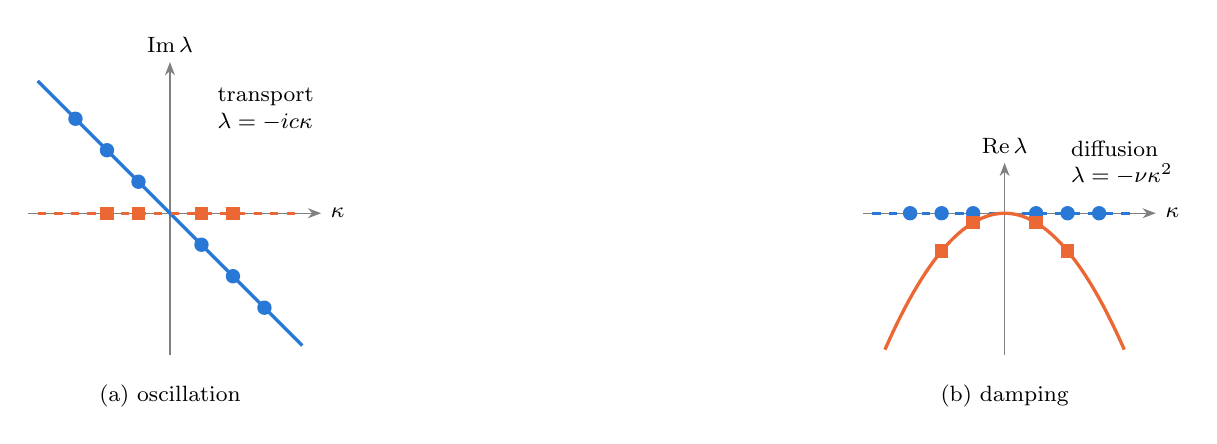
\begin{tikzpicture}[x=0.40cm,y=0.40cm,>=Stealth,font=\footnotesize]
  % (a) oscillation slice
  \begin{scope}
    \draw[->,gray] (-4.5,0)--(4.8,0) node[right,black]{$\kappa$};
    \draw[->,gray] (0,-4.5)--(0,4.8) node[above,black]{$\operatorname{Im}\lambda$};
    \draw[very thick,color={rgb,255:red,42;green,120;blue,214}] (-4.2,4.2)--(4.2,-4.2);
    \draw[very thick,color={rgb,255:red,235;green,104;blue,52},dashed] (-4.2,0)--(4.2,0);
    \foreach \k in {-3,-2,-1,1,2,3} \fill[color={rgb,255:red,42;green,120;blue,214}] (\k,-\k) circle (2.6pt);
    \foreach \k in {-2,-1,1,2} \fill[color={rgb,255:red,235;green,104;blue,52}] (\k,0) +(-2.4pt,-2.4pt) rectangle +(2.4pt,2.4pt);
    \node[anchor=west,align=left] at (1.2,3.3) {transport\\$\lambda=-ic\kappa$};
    \node at (0,-5.8) {(a) oscillation};
  \end{scope}
  % (b) damping slice
  \begin{scope}[xshift=10.6cm]
    \draw[->,gray] (-4.5,0)--(4.8,0) node[right,black]{$\kappa$};
    \draw[->,gray] (0,-4.5)--(0,1.6) node[above,black]{$\operatorname{Re}\lambda$};
    \draw[very thick,color={rgb,255:red,42;green,120;blue,214},dashed] (-4.2,0)--(4.2,0);
    \draw[very thick,color={rgb,255:red,235;green,104;blue,52},domain=-3.8:3.8,samples=60] plot (\x,{-0.3*\x*\x});
    \foreach \k in {-3,-2,-1,1,2,3} \fill[color={rgb,255:red,42;green,120;blue,214}] (\k,0) circle (2.6pt);
    \foreach \k in {-2,-1,1,2} \fill[color={rgb,255:red,235;green,104;blue,52}] (\k,{-0.3*\k*\k}) +(-2.4pt,-2.4pt) rectangle +(2.4pt,2.4pt);
    \node[anchor=west,align=left] at (1.8,1.6) {diffusion\\$\lambda=-\nu\kappa^2$};
    \node at (0,-5.8) {(b) damping};
  \end{scope}
\end{tikzpicture}
\caption{The idea of the paper on the equation $(\partial_t+c\,\partial_x)(\partial_t-\nu\,\partial_x^2)u=0$. Every Fourier mode
$e^{\lambda t+i\kappa x}$ of a solution lies on the zero set of one factor of the symbol $(\tau+c\xi)(\tau-\nu\xi^2)$: circles
on the line of the transport factor, squares on the parabola of the diffusion factor (schematic). Identifying the equation means finding these two groups.}\label{fig:branches}
\end{figure}

% ---- end sections/fig_branches.tex


\paragraph{How to read the status labels} Each statement carries one of: \proved{} (complete proof, independently reviewed), \modulo{X} (complete except for a cited published theorem~X whose source was checked), \condl{} (depends on an unverified lemma),
\openq{}, or \falsest{} (a counterexample exists). The reviewers were independent AI agents, not human referees; fifteen core algebraic theorems were additionally machine-checked in Lean~4 (branch directory \texttt{proofs/lean}). Grey tags such as \led{C3-T1}
refer to entries of the claim ledger kept with the proofs.

\paragraph{Results at a glance} \Cref{tab:results} lists the main statements; \cref{fig:dependency} shows how they depend on each other. Section~\ref{sec:theory} builds the algebra, \cref{sec:groups} proves the grouping principle and its stability,
\cref{sec:inside} treats the interaction term, \cref{sec:identify} asks when a solution determines its equation, \cref{sec:nonlin} moves to nonlinear equations, and \cref{sec:limits} collects the limits. Proofs are in \cref{app:proofs}; \cref{app:primer} is a primer.

\begin{table}[tbp]
\centering\small
\caption{Main results in the order in which they are proved. ``Proved'' means a complete proof that survived an independent review.}\label{tab:results}
\begin{tabular}{@{}p{2.6cm}p{7.4cm}p{2.6cm}@{}}
\toprule
Topic & Result & Status\\\midrule
Identification & $\Ann(u)=(P)\iff(P/P_i)(\partial)u\notin\EP$ for every irreducible $P_i\mid P$ (\cref{thm:ident}) & \proved\\
Data limits & no finite certificate; black box impossible; decidable with a bound or a holonomic model (\cref{prop:certify}) & \proved\\
Decomposition & $\ker P=\sum_j\ker Q_j$ on simply connected $\Omega$, overlap of dimension $\delta(P)$ (\cref{thm:factor}) & \proved\\
Terms vs.\ factors & a split per additive term is false in general (\cref{prop:terms}) & \proved\\
Stability & the split is stable iff $\gN>0$; for two factors, positive Friedrichs angle (\cref{thm:hm}) & \proved\\
Interaction term & $\Eint=\prod(\Id+\Delta_n)-\Id-\sum\Delta_n$; $O(N)$ value, $\Theta(2^N)$ table (\cref{thm:eint}) & \proved\\
Instability & $u_0\mapsto\Eint$ is not continuous in $H^m$ (\cref{prop:discont}) & \proved\\
Nonlinear & Burgers: closed form before the shock, sharp behaviour across it (\cref{sec:nonlin}) & \proved / \modulo{Kru\v zkov}\\
\bottomrule
\end{tabular}
\end{table}


% ---- begin sections/fig_dependency.tex
% Figure (Paper B): how the analytical results depend on each other and where the algorithm uses them.
\begin{figure}[tbp]
\centering
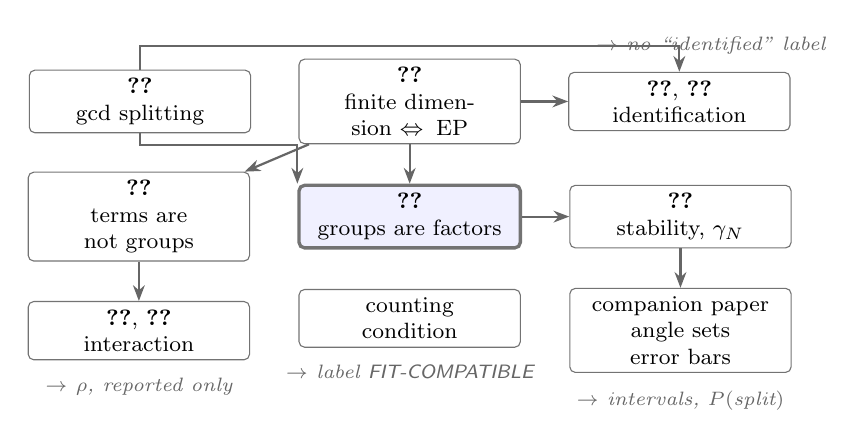
\begin{tikzpicture}[
  node distance=5mm and 6mm,
  res/.style={draw=black!55, rounded corners=2pt, align=center, font=\footnotesize, inner sep=3pt, text width=26mm},
  key/.style={res, fill=blue!6, very thick},
  use/.style={font=\scriptsize\itshape, text=black!60, align=left},
  arr/.style={-{Stealth[length=2mm]}, black!60, thick}]
\node[res] (gcd) {\cref{lem:gcd}\\gcd splitting};
\node[res, right=of gcd] (ep) {\cref{lem:ep}\\finite dimension $\Leftrightarrow\EP$};
\node[res, right=of ep] (ident) {\cref{thm:ident}, \cref{prop:unique}\\identification};
\node[key, below=of ep] (factor) {\cref{thm:factor}\\groups are factors};
\node[res, left=of factor] (terms) {\cref{prop:terms}\\terms are not groups};
\node[res, right=of factor] (hm) {\cref{thm:hm}\\stability, $\gN$};
\node[res, below=of terms] (eint) {\cref{thm:eint}, \cref{prop:discont}\\interaction};
\node[res, below=of hm] (bayes) {companion paper\\angle sets error bars};
\node[res, below=of factor] (count) {counting\\condition};
\draw[arr] (ep)--(ident); \draw[arr] (gcd.north) -- ++(0,3mm) -| (ident.north);
\draw[arr] (gcd.south) -- ++(0,-1.5mm) -| (factor.north west);
\draw[arr] (ep)--(factor); \draw[arr] (ep)--(terms); \draw[arr] (factor)--(hm); \draw[arr] (terms)--(eint); \draw[arr] (hm)--(bayes);
\node[use, below=1mm of eint] {$\to$ $\rho$, reported only};
\node[use, below=1mm of count] {$\to$ label \FC};
\node[use, below=1mm of bayes] {$\to$ intervals, $P(\text{split})$};
\node[use, above=1mm of ident, xshift=4mm] {$\to$ no ``identified'' label};
\end{tikzpicture}
\caption{How the results of \cref{sec:theory} depend on each other (arrows) and where the algorithm uses them
(italic). The shaded result is the grouping principle; everything else either prepares it or measures how well it
can be carried out on finite data.}\label{fig:dependency}
\end{figure}

% ---- end sections/fig_dependency.tex


\section{Derivatives become polynomials}\label{sec:theory}\label{ch:prelim}\label{ch:algebra}
\inbrief{Before asking what a solution knows, we turn operators into polynomials and solutions into objects that carry an ideal of equations; the one-variable case shows every idea in miniature.}

% ---- begin sections/thy_ring.tex
% Shared module: symbols, the operator ring, annihilators, the intrinsic operator.
\subsection{Derivatives become polynomials}\label{sec:ring}
Throughout, $\Omega\subset\R^2$ is a domain in the variables $(t,x)$ and every operator has constant
coefficients,
\[
  P(\partial_t,\partial_x)=\sum_{j,k}c_{jk}\,\partial_t^{\,j}\partial_x^{\,k},\qquad c_{jk}\in\C .
\]
The exponentials $\psi_{\tau,\xi}(t,x)=e^{\tau t+\xi x}$, $(\tau,\xi)\in\C^2$, are common eigenfunctions of
all such operators: $\partial_t \psi_{\tau,\xi}=\tau \psi_{\tau,\xi}$, $\partial_x \psi_{\tau,\xi}=\xi \psi_{\tau,\xi}$ and
therefore
\begin{equation}\label{eq:symbol-action}
  P(\partial)\,\psi_{\tau,\xi}=P(\tau,\xi)\,\psi_{\tau,\xi}.
\end{equation}
Differentiation is thus replaced by multiplication, and operators are replaced by polynomials.

\begin{definition}[Operator ring, symbol, characteristic variety]\label{def:ring}
The constant-coefficient operators form the commutative ring
$\ring=\C[\partial_t,\partial_x]\cong\C[\tau,\xi]$. The polynomial $P(\tau,\xi)$ is the \emph{symbol} of
$P(\partial)$, and its zero set $\Var(P)=\{(\tau,\xi)\in\C^2:P(\tau,\xi)=0\}$ is the
\emph{characteristic variety}.
\end{definition}

By \eqref{eq:symbol-action}, $\psi_{\tau,\xi}$ solves $P(\partial)u=0$ exactly when $(\tau,\xi)\in\Var(P)$.
A Fourier mode in space is the case $\xi=i\kappa$ with wavenumber $\kappa\in\R$; then
$P(\tau,i\kappa)=0$ is the \emph{dispersion relation}, and the roots $\tau=\lambda(\kappa)$ are the
temporal rates of the mode $e^{\lambda(\kappa)t+i\kappa x}$.

\paragraph{Convention}
We keep the algebraic variable $\xi$ in statements about the ring and write $\xi=i\kappa$ only when we
evaluate on Fourier modes. With this convention a symbol has real coefficients exactly when the
equation is real, and no factor $i$ ever appears inside $\ring$.

\begin{example}[Transport plus diffusion: the running example]\label{ex:tpd}
The operator $P=(\partial_t+c\,\partial_x)(\partial_t-\nu\,\partial_x^2)$, with speed $c>0$ and diffusivity
$\nu>0$, has symbol
\[
  P(\tau,\xi)=Q_1Q_2,\qquad Q_1=\tau+c\,\xi,\qquad Q_2=\tau-\nu\,\xi^2 .
\]
On Fourier modes the two factors give two dispersion branches, $\lambda_1(\kappa)=-ic\kappa$ (a
wave that travels without decay) and $\lambda_2(\kappa)=-\nu\kappa^2$ (a standing mode that decays).
A solution is any superposition of modes on the two branches. The equation is one object; its
\emph{two factors} are two groups of modes. Recovering those groups from data is the subject of this
paper. We use $c=1$, $\nu=0.3$ in all numerical illustrations.
\end{example}

\subsection{What a solution knows: the annihilator}\label{sec:ann}
A single function satisfies many equations: $e^{x}$ is annihilated by $\partial_x-1$, by
$\partial_x^2-1$ and by every multiple of $\partial_x-1$.

\begin{definition}[Annihilator]\label{def:ann}
For a distribution $u$ on $\Omega$, $\Ann(u)=\{Q\in\ring:\ Q(\partial)u=0\}$.
\end{definition}

$\Ann(u)$ is an ideal: it is closed under sums and under multiplication by any operator, because
$(SQ)(\partial)u=S(\partial)\big(Q(\partial)u\big)=0$. It collects every constant-coefficient equation
that $u$ satisfies. We use three classical facts about $\C[\tau,\xi]$~\cite{CLO15}:
unique factorization into irreducible polynomials; B\'ezout's theorem (two polynomials without a
common factor have finitely many common zeros); and Hilbert's Nullstellensatz (if $q$ vanishes on
the zero set $\Var(I)$ of an ideal $I$, then $q^k\in I$ for some $k$). All three require the complex
field, which is why symbols are always considered over $\C$.

\begin{lemma}[Splitting off the greatest common divisor]\label{lem:gcd}
Every nonzero ideal $I\subset\ring$ factors as $I=g\cdot J$, where $g=\gcdop(I)$ and $J$ is an ideal
with finite zero set $\Var(J)$.
\end{lemma}

The proof (\cref{app:proofs}) is elementary: divide by $g$, then use B\'ezout on two elements of $J$
without a common factor. Applied to $I=\Ann(u)$ the lemma gives the decomposition
\begin{equation}\label{eq:GJ}
  \Ann(u)=\Gu\,\Ju,\qquad \Gu=\gcdop\Ann(u),\qquad \sigp(u)=\Var(\Ju)\ \text{finite}.
\end{equation}
The polynomial $\Gu$ is the part of the equation that $u$ fills out along whole curves of $\C^2$;
the finite set $\sigp(u)$, the \emph{point spectrum} of $u$, lists the isolated exponentials that $u$
happens to contain. We call $\Gu$ the \emph{intrinsic operator} of $u$: it depends on $u$ alone,
whereas an annihilator $P$ supplied from outside may contain spurious factors.

\paragraph{Reading the two pieces}
The two objects in~\eqref{eq:GJ} answer different questions. The polynomial $\Gu$ is a differential
equation: its zero set $\Var(\Gu)$ is a union of curves in $\C^2$, and each curve is a continuous family of
exponential modes $e^{\tau t+\xi x}$, all solving $\Gu(\partial)v=0$. The point spectrum $\sigp(u)$ is a list: the
finitely many individual exponential modes that are present in this particular function $u$ and are not
accounted for by $\Gu$. In short, $\Gu$ identifies an equation that describes a whole family of modes;
$\sigp(u)$ identifies the isolated modes that $u$ happens to contain. \Cref{ex:extremes} shows the two
extreme cases.

\begin{example}[Two extremes]\label{ex:extremes}
For $u=e^{x}$, $\Ann(u)=(\tau,\ \xi-1)$ is the ideal of the single point $(0,1)$; hence $\Gu=1$ and
$\sigp(u)=\{(0,1)\}$: the function knows one exponential and no equation. For $u=f(x-ct)$ with a
profile $f$ that is not a finite sum of exponentials times polynomials,
$\Ann(u)=(\tau+c\xi)$; hence $\Gu=\tau+c\xi$ and $\sigp(u)=\emptyset$: the function knows its
equation completely (\cref{thm:ident}).
\end{example}

% ---- end sections/thy_ring.tex


% ---- begin sections/thy_ep.tex
% Shared module: exponential-polynomials.
\subsection{Exponential-polynomials: the solutions that remember too little}\label{sec:ep}
\begin{definition}[Exponential-polynomials]\label{def:ep}
$\EP$ is the set of finite sums $\sum_{j}p_j(t,x)\,e^{\tau_jt+\xi_jx}$ with polynomials $p_j$ and
exponents $(\tau_j,\xi_j)\in\C^2$. $\EP(\Omega)$ denotes their restrictions to $\Omega$.
\end{definition}

For a function $w$ let $\ring w=\spn\{\partial_t^{\,j}\partial_x^{\,k}w:\ j,k\ge0\}$ be the space of all its
derivatives. The map $Q\mapsto Q(\partial)w$ is onto $\ring w$ with kernel $\Ann(w)$, so
$\ring w\cong\ring/\Ann(w)$ as vector spaces.

\begin{lemma}[Finite-dimension criterion]\label{lem:ep}
Let $\Omega$ be connected. Then $w\in\EP(\Omega)$ if and only if $\dim_\C\ring w<\infty$. In that case
$\Var(\Ann w)$ is the finite set of exponents $\{(\tau_j,\xi_j)\}$ that occur in $w$.
\end{lemma}

\begin{proof}[Proof idea]
We show that $w$ is an exponential-polynomial if and only if its derivatives span a finite-dimensional
space. ($\Rightarrow$) For one term $w=p(t,x)\,e^{at+bx}$,
\[
  \partial_tw=(p_t+a\,p)\,e^{at+bx},\qquad \partial_xw=(p_x+b\,p)\,e^{at+bx}.
\]
Differentiation never raises the degree of $p$, so every derivative of $w$ lies in the finite-dimensional space
of polynomials of degree at most $\deg p$ times $e^{at+bx}$; a finite sum of such terms stays in a finite sum of
such spaces. ($\Leftarrow$) If $\ring w$ is finite-dimensional, $\partial_t$ and $\partial_x$ map it to itself and act
on it as two commuting matrices $A$ and $B$. Their minimal polynomials $m_A$ and $m_B$ give two
constant-coefficient differential equations,
\[
  m_A(\partial_t)\,w=0,\qquad m_B(\partial_x)\,w=0,
\]
one in each variable. On every rectangle inside $\Omega$ their common solutions are exponential-polynomials, and
connectedness extends this representation to all of $\Omega$. The joint eigenvalues $(a,b)$ of $A$ and $B$ are
the exponents that occur in $w$. Details are in \cref{app:proofs}.
\end{proof}

\inbrief{Deciding whether $w\in\EP$ is a finite-dimensional linear-algebra question: compute the rank
of the derivatives of $w$. The joint eigenvalues of the two matrices are the exponents, that is, the
points of $\C^2$ at which $w$ lives. This is the computational core of everything that follows: the
matrix pencil of the companion algorithm paper is exactly this eigenvalue computation, done for $\partial_t$
one wavenumber at a time.}

\begin{example}[Rich and poor solutions of the heat equation]\label{ex:heat-rich-poor}
A single heat mode $e^{-\nu\kappa^2t+i\kappa x}$ and any finite sum of such modes belong to $\EP$.
The heat kernel $t^{-1/2}e^{-x^2/(4\nu t)}$ does not: its $x$-derivatives are polynomials of
increasing degree times the same Gaussian, so they span an infinite-dimensional space.
\end{example}

% ---- end sections/thy_ep.tex


% ---- begin sections/port_ode.tex
\sectionbrief
{one variable $x$, an ODE $p(D)u=0$ with constant coefficients, $D=d/dx$, $p$ known.}
{in one variable every object of the later sections (minimal annihilator, spectral projectors, companion matrix) appears with explicit formulas and no geometry of curves.}
{prototype for Section~\ref{sec:ident} (identification) and Section~\ref{sec:groups} (the Lagrange projectors reappear as Eq.~\eqref{xeq:lagrange}).}
This section introduces, in the simplest setting, objects that reappear in Sections~\ref{sec:ident} and~\ref{sec:groups}: the minimal annihilator, the companion matrix and the spectral projectors.

\begin{notebox}{Setting and symbols}
\begin{itemize}[nosep]
\item We consider an ODE $p(D)u=0$ in one variable $x$, with $D=d/dx$ (in this section only; elsewhere $D$ is a diffusion constant).
\item The polynomial $p(\lambda)=\prod_j(\lambda-\lambda_j)^{m_j}$ has distinct roots $\lambda_j\in\C$ with multiplicities $m_j\ge1$, so that $m=\deg p=\sum_jm_j$ is the \emph{order} of the equation (not to be confused with the Sobolev index $m$ of Section~\ref{sec:groups}).
\item The set of solutions is the \emph{kernel} $\ker p(D)$, and
\[
\ker p(D)=\Big\{\sum_jq_j(x)e^{\lambda_jx}:\ \deg q_j<m_j\Big\},
\]
where each $q_j$ is a polynomial of degree $<m_j$.
\end{itemize}
\end{notebox}

\begin{aside}{Why this form}
For one root, $(D-\lambda)\big(q\,e^{\lambda x}\big)=q'e^{\lambda x}$: applying $D-\lambda$ lowers the degree of $q$ by one. Hence $(D-\lambda_j)^{m_j}$ kills $q\,e^{\lambda_jx}$ exactly when $q^{(m_j)}=0$, i.e.\ $\deg q<m_j$.

Each root therefore contributes the $m_j$ functions $x^ke^{\lambda_jx}$ ($0\le k<m_j$): these are the natural basis functions of the equation, finitely many, and together they form a basis of $\ker p(D)$, a space of dimension $m$.
\end{aside}

\begin{aside}{Example}
$p(\lambda)=(\lambda-1)^2(\lambda+2)^3$ has $\lambda_1=1$, $m_1=2$, $\lambda_2=-2$, $m_2=3$, order $m=5$. A basis of the solutions is
\[
e^{x},\quad xe^{x},\quad e^{-2x},\quad xe^{-2x},\quad x^2e^{-2x},
\]
so every solution is
\[
c_1e^{x}+c_2xe^{x}+c_3e^{-2x}+c_4xe^{-2x}+c_5x^2e^{-2x}.
\]
\end{aside}

\subsection{Identification by the Wronskian}
\begin{proposition}[{(ODE identification)}]
Let $u\in\ker p(D)$. The minimal annihilator of $u$ has degree equal to the number of independent basis functions actually present in $u$; it equals $p$ if and only if $u,u',\dots,u^{(m-1)}$ are linearly independent (nonvanishing Wronskian), i.e.\ iff every root of $p$ appears in $u$ with its full multiplicity.
\end{proposition}
\emph{Reason.} $\dimc\spn\{u,u',u'',\dots\}$ is the degree of the minimal annihilator (Lemma~\ref{lem:ep} in one variable); a missing root lowers it.

\subsection{The companion matrix and spectral form}
Write $p(\lambda)=\lambda^m+a_{m-1}\lambda^{m-1}+\dots+a_0$ (monic) and put $X=(u,u',\dots,u^{(m-1)})^{\top}$. Then $X'=CX$ with
\[
C=\begin{pmatrix}0&1&&\\&0&\ddots&\\&&\ddots&1\\-a_0&-a_1&\cdots&-a_{m-1}\end{pmatrix},\qquad
X(x)=e^{xC}X(0).
\]
The eigenvalues of $C$ are the roots of $p$. For distinct roots the matrix exponential has the spectral form
\begin{equation}\label{eq:spectral}
\begin{aligned}
e^{xC}&=\sum_{j=1}^me^{\lambda_jx}\,\Pi_j,\\
\Pi_j&=\prod_{k\ne j}\frac{C-\lambda_k\Id}{\lambda_j-\lambda_k},
\end{aligned}
\end{equation}
where the $\Pi_j$ are the Lagrange projectors onto the eigenspaces. The last row of $C$ carries the whole equation; $C$ is a \emph{matrix over the base field} for an ODE, but, as soon as the coefficients depend on $x$, or there is a second variable, its last row has entries that are operators and the object becomes a matrix over a noncommutative or polynomial ring. The invariant statement is that the whole equation corresponds to the cyclic module $\ring/\Ann(u)$ (Section~\ref{sec:theory}); the companion matrix is a way to compute with it relative to one chosen direction.

\begin{proposition}[{(Projectors of the companion matrix) \led{II-T2} \proved[]}]
The projectors $\Pi_j$ are explicit rational functions of the coefficients, with poles exactly where roots collide; they are polynomial in the coefficients if and only if the corresponding varieties are disjoint. They are \emph{not} orthogonal in general: the companion matrix is not normal for $m=2$ \falsest{} (the contrary was an early conjecture).
\end{proposition}
Hence Hilbert-space orthogonality arguments need an inner product adapted to the problem, not the standard one on the coefficient vector.

\subsection{Tensor construction versus module construction}
One may encode a PDE in a higher-order tensor of derivatives, $J=\partial_{x_{i_1}}\otimes\cdots\otimes\partial_{x_{i_n}}$, or by the companion form. The comparison, \led{Gate 3}: the \emph{principal symbol tensor} $\sigma_m(P)\in\mathrm{Sym}^m(\C^2)$ only sees the highest-order part of $P$ (for the heat operator it sees $\xi^2$ alone), so it is an invariant ``at infinity''; the \emph{cyclic module} $\ring/\Ann(u)$ is the complete invariant. All subsequent results use the module.

\begin{keypoint}
This section shows how an ODE's polynomial encodes its solution space. Its roots determine the exponential rates, their multiplicities determine the polynomial prefactors, the companion matrix represents differentiation, and spectral projectors isolate the different modes. The later sections generalize these ideas to multiple commuting derivatives, where the same structure survives but requires more algebraic machinery: the minimal annihilator becomes the ideal $\Ann(u)$ (Section~\ref{sec:ident}) and the Lagrange projectors reappear as Eq.~\eqref{xeq:lagrange} (Section~\ref{sec:groups}).
\end{keypoint}

%======================================================================

% ---- end sections/port_ode.tex


\section{Groups are factors, not terms}\label{sec:groups}\label{ch:decomp}
\inbrief{The factor decomposition, its stability measured by an angle, and the regularity of the components.}

% ---- begin sections/thy_factor.tex
% Shared module: the grouping theorem (factor decomposition), projectors, why terms fail, holes.
\subsection{Groups are factors, not terms}\label{sec:factor}
Suppose the operator is known and factored as
\begin{equation}\label{eq:factored}
  P=P_1^{e_1}\cdots P_N^{e_N},\qquad Q_j=P_j^{e_j}\ \text{pairwise coprime}.
\end{equation}
Two ways of splitting a solution suggest themselves: one piece per \emph{factor} $Q_j$, or one piece
per additive \emph{term} of the operator (for $u_t=\nu u_{xx}-cu_x$, one piece for diffusion and one
for transport). Only the first works.

\begin{theorem}[Factor decomposition]\label{thm:factor}
Let $\Omega\subset\R^2$ be bounded, connected and simply connected, and let $P$ be as in
\eqref{eq:factored}. Every $u\in\ker P(\partial)$ (in $\mathcal D'(\Omega)$ or $C^\infty(\Omega)$) can be
written
\begin{equation}\label{eq:decomp}
  u=\sum_{j=1}^N u_j,\qquad Q_j(\partial)\,u_j=0 .
\end{equation}
The tuples $(u_1,\dots,u_N)$ that sum to zero form a space of exponential-polynomials of dimension
exactly
\begin{equation}\label{eq:deltaP}
  \deltaP=\sum_{i<j}\dim_\C\ring/(Q_i,Q_j),
\end{equation}
the number of intersection points of the varieties $\Var(Q_i)$, counted pair by pair and with multiplicity.
\end{theorem}

The number $\dim_\C\ring/(Q_i,Q_j)$ therefore has two readings at once. Geometrically it counts the points where
the curves $\Var(Q_i)$ and $\Var(Q_j)$ meet, with multiplicity. Analytically it is the dimension of the space of
exponential-polynomials that solve both $Q_i$ and $Q_j$, one exponential for each meeting point (times polynomials at a
point of higher multiplicity). For two groups these are exactly the functions that can be moved from one group to the
other without changing $u$: each meeting point of the two curves is one shared mode. For three or more groups $\deltaP$
still gives the dimension of the ambiguity, but the ambiguous tuples need not be sums of modes shared by pairs.

In one variable the statement is B\'ezout's identity: if $aQ_1+bQ_2=1$, then
$u=bQ_2u+aQ_1u$ splits $u$ into a solution of $Q_1$ and a solution of $Q_2$. In two variables
``coprime'' no longer gives $1\in(Q_1,Q_2)$; it only gives finitely many common zeros, and the
finite-dimensional quotient $\ring/(Q_1,Q_2)$ measures exactly how much the two groups overlap. The
proof combines the exact sequence
$0\to\ring/(Q_1Q_2)\to\ring/(Q_1)\oplus\ring/(Q_2)\to\ring/(Q_1,Q_2)\to0$ with the vanishing of the obstruction
$\operatorname{Ext}^1(M,C^\infty(\Omega))$ for the finite-dimensional module $M=\ring/(Q_1,Q_2)$, which reduces to
$H^1_{dR}(\Omega)=0$ (compare the fundamental principle of Ehrenpreis and Palamodov~\cite{Ehr70,Pal70});
see \cref{app:proofs}.

\begin{example}[Running example: two groups with a two-dimensional overlap]\label{ex:tpd-factor}
For $Q_1=\tau+c\xi$ and $Q_2=\tau-\nu\xi^2$ the common zeros are $(0,0)$ and $(c^2/\nu,-c/\nu)$,
both simple, so $\deltaP=2$. The ambiguity is spanned by the constant function and by
$e^{(c^2/\nu)t-(c/\nu)x}$: a constant (or that growing exponential) can be moved from one group to
the other without changing $u$. Among Fourier modes ($\xi=i\kappa$, $\kappa\in\R$) only the
first point is visible: the $\kappa=0$ mode belongs to both groups.
\end{example}

\paragraph{Projectors from the eigenvalues}
When each factor is an evolution factor, $Q_j=\tau-\Lambda_j(\xi)$ with pairwise distinct branches
$\Lambda_j$, a component is an eigenfunction of $\partial_t$: $\partial_tu_j=\Lambda_j(\partial_x)u_j$. Applying
$\prod_{k\ne j}(\partial_t-\Lambda_k(\partial_x))$ to $u=\sum_lu_l$ removes every $u_l$ with $l\ne j$ and multiplies $u_j$ by $\prod_{k\ne j}(\Lambda_j-\Lambda_k)(\partial_x)$.
On a spatial Fourier mode $\kappa$ at which no two branches meet this factor is a nonzero number, hence
\begin{equation}\label{eq:lagrange}
  \hat u_j=\prod_{k\ne j}\frac{\partial_t-\Lambda_k(i\kappa)}{\Lambda_j(i\kappa)-\Lambda_k(i\kappa)}\;\hat u(t,\kappa) .
\end{equation}
This is a multiplier, rational in $\kappa$, with poles exactly where two branches
meet ($\Lambda_j(i\kappa)=\Lambda_k(i\kappa)$), that is, at the visible part of the overlap counted by $\deltaP$.
Formula~\eqref{eq:lagrange} is the Lagrange interpolation formula for the spectral projectors of a
matrix with distinct eigenvalues, applied to $\partial_t$ restricted to one wavenumber: the
\emph{eigenvalues decide the groups}. For the running example,
$\hat u_1(t,\kappa)=\big(\partial_t+\nu\kappa^2\big)\hat u/\big(\nu\kappa^2-ic\kappa\big)$, which is
singular only at $\kappa=0$.

\paragraph{Why additive terms do not form groups}
\begin{proposition}[Terms do not give components]\label{prop:terms}
If $P=\mathcal A_1+\mathcal A_2$ with constant coefficients, then
$\ker P\cap(\ker \mathcal A_1+\ker \mathcal A_2)\subseteq\ker P\cap\ker(\mathcal A_1\mathcal A_2)$, and the right-hand side is
finite-dimensional whenever $\Var(\mathcal A_1)\cap\Var(\mathcal A_2)$ is finite.
\end{proposition}

\begin{proof}
If $u=a+b$ with $\mathcal A_1a=0$ and $\mathcal A_2b=0$, then $\mathcal A_1\mathcal A_2u=\mathcal A_2\mathcal A_1a+\mathcal A_1\mathcal A_2b=0$ because the operators commute.
At a common zero of $P$ and $\mathcal A_1\mathcal A_2$ either $\mathcal A_1=0$, and then $\mathcal A_2=P-\mathcal A_1=0$, or $\mathcal A_2=0$ and then
$\mathcal A_1=0$; so $\Var(P,\mathcal A_1\mathcal A_2)=\Var(\mathcal A_1)\cap\Var(\mathcal A_2)$. When this set is finite, the ideal $(P,\mathcal A_1\mathcal A_2)$
has finite codimension, its common kernel consists of exponential-polynomials with exponents in that
set (\cref{lem:ep}), and it is finite-dimensional.
\end{proof}

For the heat equation, $\mathcal A_1=\partial_t$ and $\mathcal A_2=-\nu\partial_x^2$: every sum $f(x)+a(t)+b(t)x$ of a
solution of $\mathcal A_1$ and one of $\mathcal A_2$ is killed by $\mathcal A_1\mathcal A_2\sim\partial_t\partial_x^2$, while a heat mode
$e^{-\nu\kappa^2t}\cos\kappa x$ is not. A generic heat solution is \emph{not} ``a diffusion part plus a
stationary part''. The leftover of any term-wise split is the interaction term of
\cref{sec:eint}.

\paragraph{Where the decomposition fails}
The hypotheses of \cref{thm:factor} are not technical. On a disconnected domain different pieces
can satisfy different equations. On a domain with a hole the decomposition can fail: the Laplacian
factors as $(\partial_x+i\partial_y)(\partial_x-i\partial_y)$, yet $\log\abs{z}^2$ is harmonic on an annulus
and is not a sum of a holomorphic and an antiholomorphic single-valued function. The obstruction is
the first de Rham cohomology of $\Omega$, which is why the algorithm works on rectangles.

\roleinalg{\Cref{thm:factor} is the grouping principle of the paper. The objects that a learning
algorithm should group are \emph{modes of the same factor}; equivalently, points of the data's
Fourier--Laplace spectrum lying on the same irreducible component of $\Var(P)$. The overlap $\deltaP$
is the irreducible amount of ambiguity, and the algorithm resolves it by a fixed convention
(the companion algorithm paper).}

% ---- end sections/thy_factor.tex


% ---- begin sections/thy_cond.tex
% Shared module: conditioning of the split, Friedrichs angle, regularity.
\subsection{How well separated are the groups? The Friedrichs angle}\label{sec:cond}
\Cref{thm:factor} is algebraic: it says that the split exists, not that it is stable. Stability is a
geometric property of the component spaces $M_j=\ker_{\Hs}Q_j$, the solutions of each factor in the
Sobolev space $\Hs(\Omega)$. Let
\[
  \sumop:\ \textstyle\bigoplus_{j=1}^N M_j\to\Hs(\Omega),\qquad \sumop(u_1,\dots,u_N)=\sum_ju_j,
\]
be the \emph{sum operator}, with $\norm{(u_1,\dots,u_N)}^2=\sum_j\norm{u_j}_{\Hs}^2$, and define the
\emph{conditioning constant}
\begin{equation}\label{eq:gammaN}
  \gN=\inf_{0\ne v\perp\ker\sumop}\frac{\norm{\sumop v}^2}{\norm{v}^2}
  =\inf\sigma\big(\sumop^*\sumop\big|_{(\ker\sumop)^\perp}\big).
\end{equation}
It is the worst case, over all tuples of pieces, of the size of the sum relative to the size of the
pieces. Tuples in $\ker\sumop$ (the overlap of \cref{thm:factor}) are excluded. By the triangle and Cauchy--Schwarz inequalities,
$\norm{\sum_ju_j}^2\le\big(\sum_j\norm{u_j}\big)^2\le N\sum_j\norm{u_j}^2$, hence
\[
  0\le\gN\le N .
\]
If the spaces are mutually orthogonal, $\norm{\sum_ju_j}^2=\sum_j\norm{u_j}^2$ and $\gN=1$. At the other end, if $M_2$
approaches $M_1$ one can take $u_2\approx-u_1$: the pieces stay of unit size while their sum becomes arbitrarily
small, so $\gN\to0$. A small $\gN$ is the signature of groups that can almost cancel each other.

For two groups, $\gamma_2=1-\cF$, where the \emph{Friedrichs cosine}
\[
  \cF=\sup\big\{\abs{\ip ab}:\ a\in M_1\ominus(M_1\cap M_2),\ b\in M_2\ominus(M_1\cap M_2),\
  \norm a=\norm b=1\big\}=\cos\thetaF
\]
is the cosine of the smallest nonzero angle $\thetaF$ between the two spaces
(\cref{fig:friedrichs})~\cite{Deu01}. In regression terms, $M_1$ and $M_2$ are two blocks of regressors and $\cF$ is the
largest correlation between a combination of the first block and one of the second: the closer the blocks are to
collinear, the less the data can attribute to each.

\begin{theorem}[Stability of the split]\label{thm:hm}
Every $u\in\ker_{\Hs}P$ has components $u_j\in\Hs$ if and only if $\sum_jM_j$ is closed and dense in
$\ker_{\Hs}P$. Closedness is equivalent to $\gN>0$, and then
\begin{equation}\label{eq:stability}
  \Big(\sum_j\norm{u_j}_{\Hs}^2\Big)^{1/2}\le\gN^{-1/2}\,\norm{u}_{\Hs}
\end{equation}
for the minimum-norm components. If the component spaces are finite-dimensional, as for the sampled
kernels used by the algorithm, the sum is always closed and density holds whenever the sampled kernel of
$P$ is spanned by those of its factors, so stability reduces to $\gN>0$.
\end{theorem}

Density in $\Hs$ is a genuine condition on infinite-dimensional spaces. On convex domains solutions of
$P(\partial)u=0$ are limits of exponential solutions, uniformly on compact subsets~\cite{Mal56,Hor90},
and every exponential solution lies in $\sum_jM_j$; whether this extends to the $\Hs$ norm up to the boundary
for general $P$ we do not claim.

Two warnings come with the theorem. First, $\gN>0$ can fail on infinite-dimensional component spaces: the pieces of a smooth $u$ may then be
one derivative rougher than $u$ itself. Second, for $N\ge3$ groups the pairwise cosines do not
determine $\gN$: two pairs can be well separated while the three spaces are nearly dependent, so the
full Gram operator of $\sumop$ must be used.

\begin{figure}[tbp]
\centering
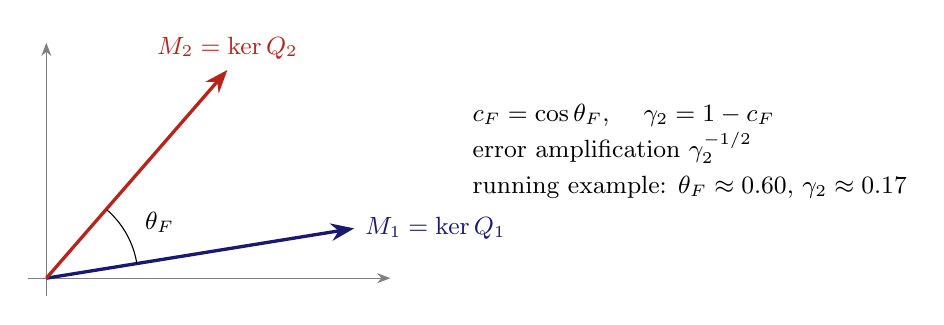
\begin{tikzpicture}[scale=1.15,>=Stealth]
  \draw[->,gray] (-0.2,0)--(3.8,0); \draw[->,gray] (0,-0.2)--(0,2.6);
  \draw[very thick,->,color=MidnightBlue] (0,0)--(3.4,0.55) node[right]{\small $M_1=\ker Q_1$};
  \draw[very thick,->,color=BrickRed] (0,0)--(2.0,2.3) node[above]{\small $M_2=\ker Q_2$};
  \draw (1.0,0.16) arc (9.2:49:1.0); \node at (1.25,0.62) {\small$\thetaF$};
  \node[anchor=west,align=left,font=\small] at (4.6,1.4)
   {$\cF=\cos\thetaF$, \quad $\gamma_2=1-\cF$\\[2pt]
    error amplification $\gamma_2^{-1/2}$\\[2pt]
    running example: $\thetaF\approx0.60$, $\gamma_2\approx0.17$};
\end{tikzpicture}
\caption{The Friedrichs angle $\thetaF$ between the solution spaces of two factors. A small angle
means that large pieces can almost cancel, so recovering the pieces from their sum amplifies errors by
up to $\gamma_2^{-1/2}=(1-\cos\thetaF)^{-1/2}$. The values quoted are those measured on the running
example in the companion algorithm paper.}\label{fig:friedrichs}
\end{figure}

\roleinalg{$\gN$ is computed on the sampled kernel bases and reported with every result.
It enters twice: as the error amplification $\gN^{-1/2}$ of the components, and through the Bayesian
split layer (the companion algorithm paper), whose credible intervals widen and whose split probability
returns to the prior as $\thetaF\to0$. A small angle is therefore never hidden: it shows up as wide
intervals, not as a confident but wrong split.}

% ---- end sections/thy_cond.tex


% ---- begin sections/port_regularity.tex
\subsection{An explicit projector for evolution factors}
For an evolution operator with $P=\prod_{j=1}^N(\tau-a_j(\xi))$ and distinct $a_j$, a component is an eigenfunction of $\partial_t$: $\partial_tu_j=a_j(\partial_x)u_j$. Applying $\prod_{k\ne j}(\partial_t-a_k(\partial_x))$ to $u=\sum_lu_l$ kills every $u_l$ with $l\ne j$ (it contains the factor $\partial_t-a_l$) and multiplies $u_j$ by $\prod_{k\ne j}(a_j-a_k)(\partial_x)$. Hence
\begin{equation}\label{xeq:lagrange}
u_j=\prod_{k\ne j}\frac{\partial_t-a_k(\partial_x)}{a_j(\partial_x)-a_k(\partial_x)}\;u ,
\end{equation}
the Lagrange formula of Eq.~\eqref{eq:spectral} with $C$ replaced by $\partial_t$. The result is a Fourier multiplier in $x$ that is rational in $\xi$, with poles where $a_j(\xi)=a_k(\xi)$; this matches the characterization ``projectors rational in $\xi$ iff the factors are coprime'' \led{II-T2/T3}.

\subsection{Where decomposition fails}
\begin{proposition}[{(Holes) \led{C12-P10} \proved[]}]\label{prop:holes}
On a domain with a hole, the decomposition fails for some $P$.
\end{proposition}
Figure~\ref{fig:hole} shows the standard obstruction. In the theorem the hypothesis ``simply connected'' means $H^1_{dR}(\Omega)=0$, exactly what removes this obstruction; a cohomological criterion for non-simply connected $\Omega$ is also available \led{OP-FUN, C12-Q6}.
\begin{figure}[!htb]
\centering
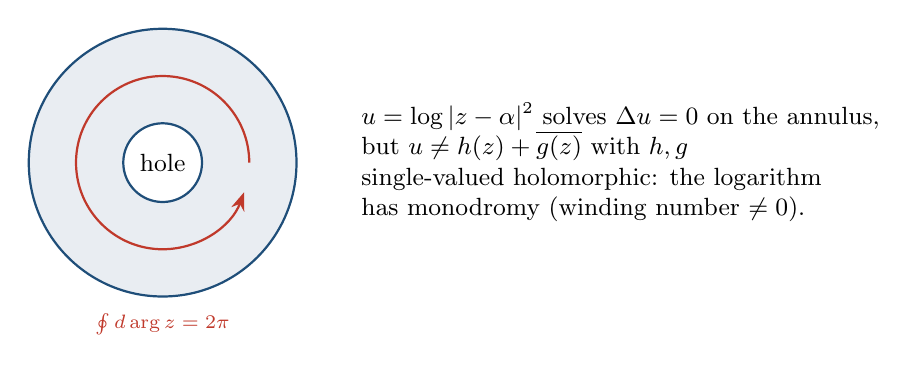
\begin{tikzpicture}
\fill[cA!10] (0,0) circle (1.7); \fill[white] (0,0) circle (0.5);
\draw[cA,thick] (0,0) circle (1.7); \draw[cA,thick] (0,0) circle (0.5);
\node at (0,0) {\small hole};
\draw[cB,thick,-{Stealth}] (1.1,0) arc (0:340:1.1);
\node[cB,font=\scriptsize] at (0,-2.05) {$\oint d\arg z=2\pi$};
\node[align=left,font=\small,anchor=west] at (2.4,0) {$u=\log|z-\alpha|^2$ solves $\Delta u=0$ on the annulus,\\ but $u\neq h(z)+\overline{g(z)}$ with $h,g$\\ single-valued holomorphic: the logarithm\\ has monodromy (winding number $\neq0$).};
\end{tikzpicture}
\caption{The Laplacian $\partial_x^2+\partial_y^2=(\partial_x+i\partial_y)(\partial_x-i\partial_y)$ factors, but the factor decomposition fails on a punctured disc: the obstruction is topological ($H^1_{dR}\neq0$).}\label{fig:hole}
\end{figure}

\subsection{Regularity: when are the components in $H^m$?}\label{ch:regular}
The decomposition is an algebraic statement; analysis enters when we want components in a Sobolev space. For two components the governing condition is geometric: the two component spaces $M_1$ and $M_2$ must be separated by a positive angle (Figure~\ref{xfig:friedrichs}); the next theorem makes this precise for any number of components. Two difficulties appear along the way; they are collected in the box after the theorem.
\begin{proposition}[{(Loss of a derivative) \led{C12-C1} \falsest}]\label{prop:loss}\label{cex:loss}
``If $u\in H^m(\Omega)$ then all $u_j\in H^m$'' is false: one derivative can be lost. In other words, the pieces of a smooth function may be rougher than the function itself.
\end{proposition}
\begin{theorem}[{(Regularity criterion) \led{C12-T3, C12-P7} \proved[]}]\label{xthm:hm}
All components lie in $H^m$ for every $u\in\ker_{H^m}P$ iff the sum $\sum_j\ker_{H^m}Q_j$ is \emph{closed} and \emph{dense} in $\ker_{H^m}P$. Closedness is equivalent to $\gamma_N>0$, where
\[
\begin{aligned}
\gamma_N&=\inf\sigma\big(S^*S\big|_{(\ker S)^\perp}\big),\\
S&:\bigoplus_{j=1}^N\ker Q_j\to H^m,\qquad S(u_1,\dots,u_N)=\sum_{j=1}^Nu_j .
\end{aligned}
\]
For $N=2$ this is the condition $c_F<1$ on the Friedrichs cosine. Density holds on every bounded convex $\Omega$, for every $P$ and $m$ \led{OPF5B-T1} \modulo{H\"ormander~\cite{ho}, Stein}.
\end{theorem}
\begin{notebox}{Reading $\gamma_N$}
\begin{itemize}[nosep]
\item The space $\bigoplus_j\ker Q_j$ consists of the $N$-tuples $v=(u_1,\dots,u_N)$ with norm $\|v\|^2=\sum_j\|u_j\|_{H^m}^2$;
\item $Sv=\sum_ju_j$ is their sum;
\item $S^*$ is the adjoint of $S$;
\item $(\ker S)^\perp$ removes the tuples that sum to zero (the ambiguity of Theorem~\ref{thm:factor});
\item $\inf\sigma$ is the bottom of the spectrum.
\end{itemize}
Since $S^*S$ restricted to $(\ker S)^\perp$ is self-adjoint and nonnegative, the bottom of its spectrum is the minimum of the Rayleigh quotient
\[
\frac{\langle S^*Sv,v\rangle}{\|v\|^2}=\frac{\|Sv\|^2}{\|v\|^2}.
\]
Hence the formula of the theorem is equivalent to the more intuitive
\[
\boxed{\ \gamma_N=\inf_{\substack{v\in(\ker S)^\perp\\ v\ne0}}\frac{\|Sv\|_{H^m}^2}{\|v\|^2}\ }
\]
\end{notebox}

\begin{aside}{In words}
$\gamma_N$ is the worst case, over all tuples of pieces, of the ratio between the size of the sum and the size of the pieces.
\begin{itemize}[nosep]
\item If $\gamma_N>0$ the pieces cannot nearly cancel each other, and
\[
\|v\|\le\gamma_N^{-1/2}\|Sv\|:
\]
the pieces are controlled by the sum, so recovering them from $u$ is stable.
\item If $\gamma_N\to0$ there are large pieces whose sum is tiny, and the recovery is unstable.
\end{itemize}
\textbf{The case $N=2$.} One finds $\gamma_2=1-c_F$, where
\[
c_F=\sup\{|\langle a,b\rangle|:\ a\in M_1\ominus(M_1\cap M_2),\ b\in M_2\ominus(M_1\cap M_2),\ \|a\|=\|b\|=1\}
\]
is the Friedrichs cosine: the part of $v$ lying in $M_1\cap M_2$ contributes the ratio $2$ and does not affect the infimum, and on the rest
\[
\|a+b\|^2\ge(1-c_F)(\|a\|^2+\|b\|^2)
\]
with near-equality attained. Hence $c_F<1\iff\gamma_2>0$, as stated.
\end{aside}
\begin{figure}[!htb]
\centering
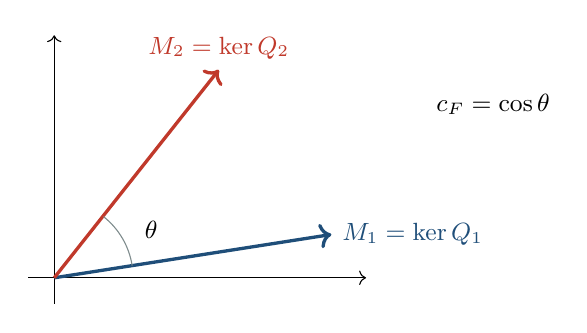
\begin{tikzpicture}[scale=1.1]
\draw[->] (-0.3,0)--(3.6,0); \draw[->] (0,-0.3)--(0,2.8);
\draw[cA,very thick,->] (0,0)--(3.2,0.5) node[right,font=\small]{$M_1=\ker Q_1$};
\draw[cB,very thick,->] (0,0)--(1.9,2.4) node[above,font=\small]{$M_2=\ker Q_2$};
\draw[cG] (0.9,0.14) arc (8.9:51.6:0.9); \node[font=\small] at (1.12,0.55) {$\theta$};
\node[font=\small,anchor=west] at (4.3,2.0) {$c_F=\cos\theta$};



\end{tikzpicture}
\caption{Friedrichs angle $\theta$ between two component spaces $M_1=\ker Q_1$ and $M_2=\ker Q_2$. A larger angle means a better-conditioned recovery of the pieces from their sum.}\label{xfig:friedrichs}
\end{figure}
For $N=2$, Figure~\ref{xfig:friedrichs} reads as follows: $c_F=\cos\theta$; if $\theta>0$ the sum $M_1+M_2$ is closed and the pieces depend continuously on $u$; as $\theta\to0$ the split becomes unstable. For $N\ge3$ the pairwise angles do not suffice; $\gamma_N$, the smallest nonzero eigenvalue of $S^*S$, is the right conditioning number: it is the conditioning of the linear map ``components $\mapsto$ sum'', exactly like the smallest nonzero singular value in a least-squares problem.

\begin{caution}[title=Two problems with regularity]
\textbf{Problem 1: stability \falsest.} Algebraically the split always exists (Theorem~\ref{thm:factor}), but the pieces may be less regular than $u$. When the angle between the component spaces tends to $0$ (that is, $\gamma_N\to0$) the map ``$u\mapsto$ pieces'' becomes unstable, and one derivative can be lost (Proposition~\ref{prop:loss}). For the algorithm: check $\gamma_N>0$ before using the components in $H^m$ (Step~5).\\[3pt]
\textbf{Problem 2: three or more components \openq.} For $N\ge3$ the pairwise cosines $c_F(i,j)$ do not decide whether the sum of kernels is closed: an abstract Hilbert-space counterexample exists \led{S-CHECK-4}, and whether it can occur for differential operators is open \led{C12-Q2}.
\end{caution}

\begin{takeaway}
Algebraically the split always exists (Theorem~\ref{thm:factor}); analytically, the components are well behaved exactly when the component spaces are separated by a positive angle (Theorem~\ref{xthm:hm}). The next section stops asking for a split into factors and asks what survives when one splits by additive terms instead.
\end{takeaway}

%======================================================================

% ---- end sections/port_regularity.tex


\section{Inside one group: the interaction term}\label{sec:inside}\label{ch:interaction}
\inbrief{What remains when a factor is built from several terms: an exact formula, its cost, its instability, and what happens when the terms do not commute.}

% ---- begin sections/thy_eint.tex
% Shared module: interaction term and energy.
\subsection{Inside one group: the interaction term and its energy}\label{sec:eint}
A single factor may have several additive terms: $Q_2=\tau-\nu\xi^2$ has one, but the advection--diffusion
factor $\tau+c\xi-\nu\xi^2$ has two. \Cref{prop:terms} says that such a factor cannot be split further
into one solution per term. We now measure exactly what is left over.

Consider an evolution $u_t=\mathcal Au$ with $\mathcal A=\mathcal A_1+\dots+\mathcal A_K$ (the terms), the flow $\flow(t)=e^{t\mathcal A}$ and the
flows of the single terms $\flow_n(t)=e^{t\mathcal A_n}$. If term $n$ acted alone it would change the datum by
$\Delta_nu_0=(\flow_n(t)-\Id)u_0$. The \emph{interaction term} is the part of the evolution that is not
the sum of these single-term changes,
\begin{equation}\label{eq:eint-def}
  \Eint(t)=u(t)-u_0-\sum_{n=1}^K\big(\flow_n(t)u_0-u_0\big).
\end{equation}

\begin{theorem}[Interaction term]\label{thm:eint}
If the terms commute (in particular, for constant coefficients),
\[
  \Eint(t)=\Big[\prod_{n=1}^K(\Id+\Delta_n)-\Id-\sum_{n=1}^K\Delta_n\Big]u_0
  =\sum_{\mathcal E\subseteq\{1,\dots,K\},\ \abs{\mathcal E}\ge2}\Big(\prod_{n\in\mathcal E}\Delta_n\Big)u_0 .
\]
For two terms $\Eint=\Delta_1\Delta_2u_0$. On Fourier modes, with symbols $\hat{\mathcal A}_n(\kappa)$ of the terms,
\begin{equation}\label{eq:eint-fourier}
  \widehat{\Eint}(t,\kappa)=\Big[\prod_ne^{t\hat{\mathcal A}_n(\kappa)}-1-\sum_n\big(e^{t\hat{\mathcal A}_n(\kappa)}-1\big)\Big]\hat u_0(\kappa).
\end{equation}
\end{theorem}

\begin{proof}
Commuting terms give $\flow=\prod_n\flow_n=\prod_n(\Id+\Delta_n)$. Expanding the product over subsets
$\mathcal E\subseteq\{1,\dots,K\}$ and removing the subsets with zero or one element gives the formula; on
Fourier modes every operator is multiplication by a number.
\end{proof}

Formula~\eqref{eq:eint-fourier} costs $O(K)$ operations per wavenumber, although writing out all
cross terms would need $2^K-K-1$ of them. For advection--diffusion,
$\abs{\widehat{\Eint}}/\abs{\hat u_0}=\abs{(e^{-ic\kappa t}-1)(e^{-\nu\kappa^2t}-1)}\le2$: the interaction
is of the same size as the solution, so it is not a small correction that a regularizer could remove.

\begin{proposition}[No stable removal]\label{prop:discont}\label{thm:noreg}\label{thm:nocont}
Let $Q=\tau+c\xi-\nu\xi^2$ (advection--diffusion, terms $-c\partial_x$ and $\nu\partial_x^2$) on a bounded
rectangle $\Omega=(0,T)\times(a,b)$. For every $s\ge0$,
\[
  \sup\Big\{\norm{\Eint}_{L^2(\Omega)}/\norm{u}_{\Hs(\Omega)}:\ u\in\EP,\ Q(\partial)u=0,\ u\ne0\Big\}=\infty,
\]
so $u\mapsto\Eint$ has no continuous extension to $\ker_{\Hs}Q$. Moreover, a solution of $Q(\partial)u=0$ is a
sum $v+w$ of solutions of the single-term evolutions $(\partial_t+c\partial_x)v=0$ and $(\partial_t-\nu\partial_x^2)w=0$ only
if it lies in a finite-dimensional space of exponential-polynomials.
\end{proposition}

The test solutions are $e^{\lambda_\zeta t+\zeta x}$ with real $\zeta>c/\nu$ and $\lambda_\zeta=\nu\zeta^2-c\zeta$, legitimate
data on a bounded interval: diffusion alone amplifies them by $e^{\nu\zeta^2t}$, the solution grows only like
$e^{\lambda_\zeta t}$, and the interaction must cancel a difference that grows faster than any power of $\zeta$
(\cref{app:proofs}). On a periodic domain with bounded wavenumbers the Fourier multiplier above is bounded by
$2$; the instability comes from the non-periodic window, which is the situation of real data. The second
statement means that a model which writes the data as a sum of single-term pieces, with any penalty on the
pieces, leaves a remainder on generic data, and that remainder is the interaction.

\paragraph{Energy}
We measure the size of a group and of the interaction by $L^2$ energies on the observation window.
The \emph{energy share} of group $j$ and the \emph{interaction ratio} are
\begin{equation}\label{eq:energy}
  w_j=\frac{\norm{u_j}}{\sum_k\norm{u_k}},\qquad
  \rho=\frac{\norm{\Eint(T)}}{\norm{u(T)-u_0}} ,
\end{equation}
where $T$ is the length of the time window. The shares $w_j$ say how much of the data each group
explains; $\rho$ says how far the evolution inside a multi-term factor is from the superposition of its
terms ($\rho=0$ for a factor with a single term). Interactions occur only \emph{inside} a factor:
different factors superpose exactly, which is another way of saying that factors, not terms, are the
right groups.

\roleinalg{By \cref{prop:discont}, a value of $\Eint$ computed from one interpolated field on a
bounded window is not reliable. The algorithm reports the distribution of $\rho$ over posterior samples
(the companion algorithm paper), never a single number, and uses the shares $w_j$ with credible intervals.}

% ---- end sections/thy_eint.tex


% ---- begin sections/port_terms.tex
\subsection{Definition via the flows of the single terms}
Let $S(t)=e^{tA}$ and $S_n(t)=e^{tA_n}$. The contribution that term $n$ \emph{alone} would make to the solution is $S_n(t)u_0-u_0$. The remainder is the interaction term
\begin{equation}\label{xeq:eint-def}
\Eint^{\mathrm{add}}(t)=u(t)-u_0-\sum_{n=1}^N\big(S_n(t)u_0-u_0\big).
\end{equation}
(The superscript ``add'' records that this is the \emph{additive} definition; below we write $\Eint$ for $\Eint^{\mathrm{add}}$ unless the distinction matters.)

\subsection{Exact formula in the commuting case}
\begin{aside}{Why constant coefficients commute, and what $\Delta_n$ is}
Constant-coefficient operators are polynomials in $\partial_t,\partial_x$ (Section~\ref{sec:theory}) and the ring $\ring$ is commutative, so any two terms commute: $A_1A_2=A_2A_1$. For commuting operators
\[
e^{t(A_1+A_2)}=e^{tA_1}e^{tA_2},\qquad\text{hence}\qquad S=\prod_nS_n;
\]
without commutativity this fails (Section~\ref{sec:noncomm}).

We call
\[
\Delta_n=S_n(t)-\Id
\]
the \emph{increment} produced by term $n$ alone, where $\Id$ is the identity operator and $t$ is fixed; thus $S_n=\Id+\Delta_n$, and $\Delta_nu_0=S_n(t)u_0-u_0$ is exactly the contribution of term $n$ in \eqref{xeq:eint-def}. Products of operators are compositions.
\end{aside}

\begin{notebox}{Fourier variables}
For constant coefficients it is convenient to pass to Fourier variables. With
\[
\hat u(\kappa)=\int u(x)e^{-i\kappa x}\dd x,
\]
where $\kappa\in\R$ is the frequency:
\begin{itemize}[nosep]
\item the derivative $\partial_x$ becomes multiplication by $i\kappa$;
\item each term $A_n$ becomes multiplication by its \emph{symbol} $a_n(\kappa)$ (a polynomial in $i\kappa$);
\item $e^{tA_n}$ becomes multiplication by the number $e^{ta_n(\kappa)}$.
\end{itemize}
Operators turn into numbers and compositions into products of numbers, so for a fixed $\kappa$ every computation below is scalar.
\end{notebox}
\begin{theorem}[{(Interaction term) \led{P1-T2, P1-T3} \proved[]}]\label{xthm:eint}
Assume the $A_n$ commute (e.g.\ constant coefficients). Write $\Delta_n=S_n(t)-\Id$. Then
\begin{equation}\label{eq:eint}
\Eint^{\mathrm{add}}=\Big[\prod_{n=1}^N(\Id+\Delta_n)-\Id-\sum_{n=1}^N\Delta_n\Big]u_0 .
\end{equation}
For $N=2$ this is simply $\Eint=\Delta_1\Delta_2u_0=(S_1-\Id)(S_2-\Id)u_0$. In Fourier variables, with $\hat A_n=a_n(\kappa)$,
\[
\widehat{\Eint}(t,\kappa)=\Big[\prod_n\big(e^{ta_n(\kappa)}\big)-1-\sum_n\big(e^{ta_n(\kappa)}-1\big)\Big]\hat u_0(\kappa).
\]
\end{theorem}
\begin{proof}
Commutation gives $S=e^{t\sum A_n}=\prod_nS_n$. Substitute $S_n=\Id+\Delta_n$ in \eqref{xeq:eint-def}. For $N=2$, expand the product:
\[
\begin{aligned}
S_1S_2&=(\Id+\Delta_1)(\Id+\Delta_2)\\
&=\Id+\Delta_1+\Delta_2+\Delta_1\Delta_2 ,
\end{aligned}
\]
and $\sum_n(S_n-\Id)=\Delta_1+\Delta_2$, so the remainder in \eqref{xeq:eint-def} is $\Delta_1\Delta_2u_0$.

For general $N$, the $\Delta_n$ commute, so
\[
\prod_n(\Id+\Delta_n)=\sum_{S\subseteq\{1,\dots,N\}}\prod_{n\in S}\Delta_n ;
\]
removing the subsets with $|S|=0$ and $|S|=1$ leaves
\[
\Eint=\sum_{|S|\ge2}\Delta_S\,u_0,\qquad \Delta_S=\prod_{n\in S}\Delta_n .
\]
In words: the interaction is the sum of products of at least two increments, and appears only when at least two terms act together.
\end{proof}

\paragraph{A concrete case.}\label{par:advdiff}
Take advection--diffusion, $u_t=-cu_x+Du_{xx}$, with Gaussian datum $u_0=g(x;\sigma^2)$, where $g(x;v)=e^{-x^2/2v}/\sqrt{2\pi v}$. The two flows act as a translation and a Gaussian smoothing:
\[
S_1u_0=g(x-ct;\sigma^2),\qquad S_2u_0=g(x;s^2),\qquad u=g(x-ct;s^2),\qquad s^2=\sigma^2+2Dt .
\]
Hence
\[
\Eint=g(x-ct;s^2)-g(x-ct;\sigma^2)-g(x;s^2)+g(x;\sigma^2).
\]
Figure~\ref{fig:eint}(a) plots it: it is comparable in size to $u$ itself, so it cannot be discarded as a small correction. In Fourier variables the ratio $|\widehat{\Eint}|/|\hat u_0|=|(e^{-ic\kappa t}-1)(e^{-D\kappa^2t}-1)|$ is at most $2$; it vanishes at $\kappa=0$ and whenever $c\kappa t\in2\pi\mathbb Z$ (the translation returns to the identity), see Figure~\ref{fig:eint}(b).

\begin{figure}[!htb]
\centering
\begin{tikzpicture}
\begin{axis}[width=7.6cm,height=5.6cm,xlabel={$x$},xmin=-6,xmax=8,ymin=-0.2,ymax=0.45,
 title={\small (a) $u_t=-cu_x+Du_{xx}$, $t=1$, $c=2$, $D=\tfrac12$},legend style={font=\scriptsize,draw=none,fill=white,fill opacity=0.8,text opacity=1,at={(0.02,0.98)},anchor=north west},
 domain=-6:8,samples=140,no markers]
\addplot[cG,thick,dashed] {gauss(x,1)};
\addplot[cA,thick] {gauss(x-2,2)};
\addplot[cB,very thick] {gauss(x-2,2)-gauss(x-2,1)-gauss(x,2)+gauss(x,1)};
\legend{$u_0$,$u(t)$,$\Eint$}
\end{axis}
\end{tikzpicture}\hfill
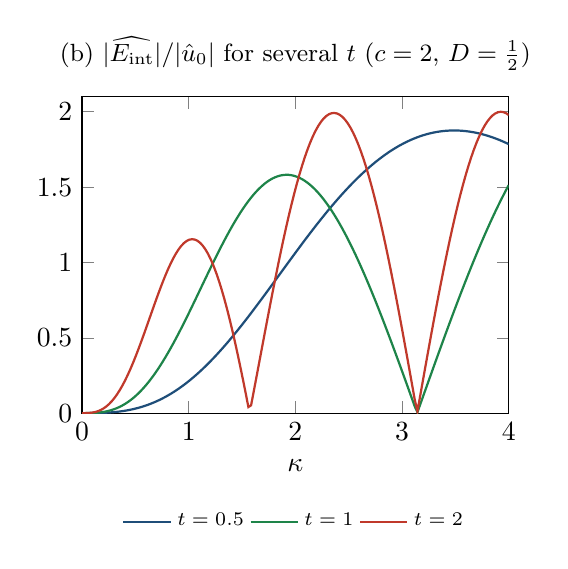
\begin{tikzpicture}
\begin{axis}[width=7.0cm,height=5.6cm,xlabel={$\kappa$},xmin=0,xmax=4,ymin=0,ymax=2.1,
 title={\small (b) $|\widehat{\Eint}|/|\hat u_0|$ for several $t$ ($c=2$, $D=\tfrac12$)},legend style={font=\scriptsize,draw=none,at={(0.5,-0.28)},anchor=north,legend columns=3},
 domain=0:4,samples=160,no markers]
\addplot[cA,thick] {sqrt(((cos(deg(2*0.5*x))-1)^2+sin(deg(2*0.5*x))^2)*(exp(-0.5*0.5*x^2)-1)^2)};
\addplot[cC,thick] {sqrt(((cos(deg(2*1.0*x))-1)^2+sin(deg(2*1.0*x))^2)*(exp(-0.5*1.0*x^2)-1)^2)};
\addplot[cB,thick] {sqrt(((cos(deg(2*2.0*x))-1)^2+sin(deg(2*2.0*x))^2)*(exp(-0.5*2.0*x^2)-1)^2)};
\legend{$t=0.5$,$t=1$,$t=2$}
\end{axis}
\end{tikzpicture}
\caption{Advection--diffusion with Gaussian datum ($\sigma^2=1$, $c=2$, $D=\tfrac12$). (a) $u_0$, $u(t)$ and $\Eint$ at $t=1$. (b) The Fourier ratio $|\widehat{\Eint}|/|\hat u_0|$ for three times.}\label{fig:eint}
\end{figure}

\subsection{Cost: $O(N)$ versus $2^N$}
Expanding \eqref{eq:eint} in the $\Delta_n$ produces one monomial per subset of $\{1,\dots,N\}$ with at least two elements: $2^N-N-1$ cross terms (Figure~\ref{fig:lattice}: the red nodes are the cross terms). Writing the \emph{complete table} of cross terms is therefore exponential. Evaluating a \emph{value} is cheap, because we never expand the product. The algorithm uses exactly the product (Fourier) form of Theorem~\ref{xthm:eint},
\[
\widehat{\Eint}(t,\kappa)=\Big[\prod_{n=1}^Ne^{ta_n(\kappa)}-1-\sum_{n=1}^N\big(e^{ta_n(\kappa)}-1\big)\Big]\hat u_0(\kappa),
\]
which for a fixed $\kappa$ needs the $N$ numbers $e^{ta_n(\kappa)}$, $N-1$ products and $N$ subtractions: $O(N)$ operations once $\hat u_0(\kappa)$ is known.
\begin{aside}{Two remarks on cost}
\textbf{What ``value'' means.} Here ``value'' means one Fourier value; recovering $\Eint(t,x)$ at a point of space needs an inverse Fourier transform, whose cost is not counted in the $O(N)$.

\textbf{Where $2^N$ comes from.} The count $2^N-N-1$ refers only to writing out all cross terms one by one; the product form never does so (Step~6 of the algorithm).
\end{aside}
\begin{figure}[!htb]
\centering
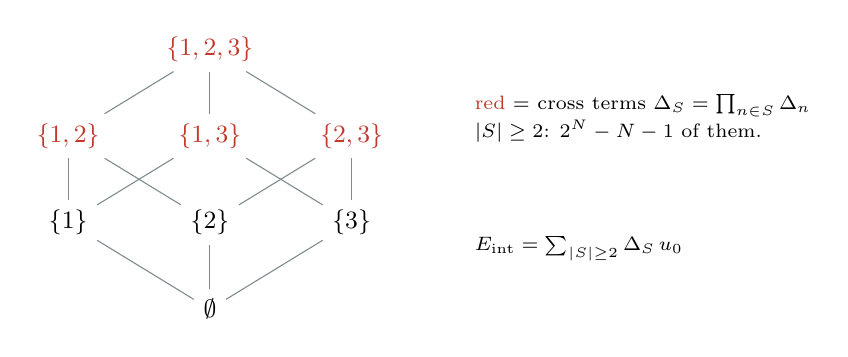
\begin{tikzpicture}[x=1.8cm,y=1.1cm,every node/.style={font=\small}]
\node (e) at (0,0) {$\emptyset$};
\node (1) at (-1,1) {$\{1\}$}; \node (2) at (0,1) {$\{2\}$}; \node (3) at (1,1) {$\{3\}$};
\node[text=cB] (12) at (-1,2) {$\{1,2\}$}; \node[text=cB] (13) at (0,2) {$\{1,3\}$}; \node[text=cB] (23) at (1,2) {$\{2,3\}$};
\node[text=cB] (123) at (0,3) {$\{1,2,3\}$};
\foreach \a/\b in {e/1,e/2,e/3,1/12,1/13,2/12,2/23,3/13,3/23,12/123,13/123,23/123} \draw[cG] (\a)--(\b);
\node[anchor=west,align=left,font=\scriptsize] at (1.8,2.2) {\textcolor{cB}{red} = cross terms $\Delta_S=\prod_{n\in S}\Delta_n$\\ $|S|\ge2$: $2^N-N-1$ of them.};
\node[anchor=west,align=left,font=\scriptsize] at (1.8,0.7) {$\Eint=\sum_{|S|\ge2}\Delta_S\,u_0$};
\end{tikzpicture}
\caption{Subset lattice for $N=3$ terms: one node per subset $S$ of terms, one monomial $\Delta_S$ per node with $|S|\ge2$. The count $2^N-N-1$ is what makes the full table exponential.}\label{fig:lattice}
\end{figure}
\begin{proposition}[{(Complexity) \led{P1-T3} \proved[]}]
In the commuting exponential-type class, a value of $\Eint$ costs $O(M(N+\sum d))$ for $M$ evaluation points; aggregated by order $O(MN^2)$; the full table $\Theta(M2^N(L+1)^2)$.
\end{proposition}
\edmark{E1}


% ---- end sections/port_terms.tex


% ---- begin sections/port_tdpt.tex
\subsection{Time-dependent perturbation theory}
\begin{aside}{Why this subsection}
The product formula \eqref{eq:eint} needs commuting terms. When terms do not commute, or when boundary conditions are imposed, there is no closed formula, but $\Eint$ is still defined by \eqref{xeq:eint-def}. Perturbation theory expands the flow in powers of the interaction. From this expansion one reads
\begin{enumerate}[nosep,label=(\roman*)]
\item that $\Eint$ is well defined for all times (convergence),
\item approximations obtained by truncating the series order by order, and
\item the size of $\Eint$ for small $t$.
\end{enumerate}
\end{aside}

Split $A=A_1+B$, where $A_1$ is the principal term (for instance diffusion) and $B$, the remaining terms, is treated as a perturbation of $A_1$. The Dyson--Phillips series is
\begin{equation}\label{eq:dyson}
\begin{aligned}
S(t)&=\sum_{k\ge0}S^{(k)}(t),\\
S^{(0)}(t)&=e^{tA_1},\\
S^{(k+1)}(t)&=\int_0^te^{(t-s)A_1}\,B\,S^{(k)}(s)\dd s ,
\end{aligned}
\end{equation}
the same expansion that gives the interaction picture of quantum mechanics~\cite{dy}.

\begin{aside}{Reading the series}
\begin{itemize}[nosep]
\item $S^{(0)}=e^{tA_1}$ is the flow of $A_1$ alone;
\item $S^{(k)}$ collects the contributions in which $B$ acts $k$ times, at intermediate times $s\in(0,t)$, with the flow of $A_1$ in between.
\end{itemize}
The terms with $k\ge1$ are therefore the part of the flow in which $B$ acts on the evolution generated by $A_1$, that is, the interaction. (When $A_1$ and $B$ commute, the first-order term is
\[
\int_0^te^{(t-s)A_1}Be^{sA_1}\dd s=t\,Be^{tA_1},
\]
consistent with Section~\ref{sec:inside}.)
\end{aside}

\textbf{What it gives.} The series converges for all $t$ when $A_1$ generates an even-order dissipative semigroup (e.g.\ diffusion) and $B$ is a lower-order $L^\infty$ perturbation, also with Dirichlet conditions \led{P3-T1} \modulo{Miyadera--Voigt~\cite{en}}: so $\Eint$ is well defined and can be approximated by truncation even without a closed formula. Each $S^{(k)}$ is the order-$k$ part of the interaction. For small times, for boundary-induced interaction, with $k$ the order of contact of the datum with the boundary, $\|\Eint\|\sim t^{k/2+3/4}$ \led{P3-T3, OP-F5A} \proved\edmark{E10}: the smoother the datum is against the boundary (larger $k$), the faster the interaction becomes negligible as $t\to0$.

\subsection{Non-commuting terms}\label{sec:noncomm}
If $[A_1,A_2]\ne0$, then $e^{t(A_1+A_2)}\neq e^{tA_1}e^{tA_2}$; by Baker--Campbell--Hausdorff,
\[
e^{tA_1}e^{tA_2}=\exp\!\Big(t(A_1+A_2)+\tfrac{t^2}{2}[A_1,A_2]+O(t^3)\Big).
\]
\begin{proposition}[{(Lie-algebra dichotomy) \led{P1-T4, P1-T5} \proved[]}]\label{thm:lie}
If the Lie algebra generated by the terms is solvable, an exact formula with finitely many scalar functions exists (Wei--Norman). Otherwise only a local expansion exists, and \textbf{no finite product of the flows of the individual terms} reproduces $e^{t(X+\varepsilon Y)}$.
\end{proposition}
\begin{takeaway}
For commuting terms the interaction is explicit and cheap to evaluate, but it cannot be made to vanish nor be computed stably in $H^m$; for non-commuting terms even the explicit form is lost in general. These are the linear-case limits against which the nonlinear extension of Section~\ref{sec:nonlin} must be read.
\end{takeaway}

%======================================================================

% ---- end sections/port_tdpt.tex


\section{When does a solution determine its equation?}\label{sec:identify}\label{ch:ident}
\inbrief{The identification criterion, uniqueness, and what finite data can and cannot certify. This explains why the algorithm of the companion paper never reports ``identified''.}

% ---- begin sections/thy_ident.tex
% Shared module: identification, uniqueness, the spectral form, limits of certification.
\subsection{When does a solution determine its equation?}\label{sec:ident}
Let $\Omega$ be open and connected (on a disconnected set the pieces may obey different equations),
let $u\in\mathcal D'(\Omega)$ satisfy $P(\partial)u=0$, and let $P=\prod_iP_i^{e_i}$ (up to a nonzero constant factor) be the
factorization of $P$ into pairwise non-associate irreducible polynomials $P_i$ with multiplicities
$e_i$. The question is whether $\Ann(u)=(P)$: then every constant-coefficient equation satisfied by
$u$ is a consequence of $P$, and $P$ is determined by $u$.

\begin{theorem}[Identification criterion]\label{thm:ident}
Put $v_i=(P/P_i)(\partial)\,u$ and $v_i'=(P/P_i^{e_i})(\partial)\,u$.
\begin{enumerate}[label=(\alph*)]
  \item $\Ann(u)=(P)$ if and only if $v_i\notin\EP(\Omega)$ for every $i$.
  \item $\Var(\Ann u)=\Var(P)$ if and only if $v_i'\notin\EP(\Omega)$ for every $i$.
  \item If $P$ is square-free, (a) and (b) coincide. If $P$ is monic in $\tau$ of degree $m$, then
  $\Ann(u)=(P)$ if and only if the only $(\varphi_0,\dots,\varphi_{m-1})\in\C[\xi]^m$ with
  $\sum_{j<m}\varphi_j(\partial_x)\,\partial_t^{\,j}u=0$ is zero.
\end{enumerate}
\end{theorem}

The idea is to strip one irreducible factor and look at what is left. The function $v_i$ solves
$P_i(\partial)v_i=0$. If $v_i$ is a generic solution of that factor, no smaller operator kills $u$.
If $v_i$ is an exponential-polynomial, some $h$ coprime to $P_i$ kills it, and then
$h\cdot P/P_i$ is an annihilator of $u$ that is not a multiple of $P$. The converse uses
\cref{lem:gcd}; the full proof is in \cref{app:proofs}.

\begin{proposition}[Uniqueness and the intrinsic operator]\label{prop:unique}
\begin{enumerate}[label=(\alph*)]
  \item If $\Ann(u)=(P)$, then $P$ is determined by $u$ up to a nonzero constant and is the unique
  annihilator of minimal degree.
  \item $\Ann(u)=(P)$ if and only if $\sigp(u)=\emptyset$ and $\Gu\sim P$ (equality up to a constant).
  \item For any annihilator $P$, the multiplicity of $P_i$ in $\Gu$ equals $e_i-\max\{k\le e_i:
  (P/P_i^{k})(\partial)u\in\EP\}$. Hence $\Gu$ is computed from any annihilator by at most
  $\sum_ie_i$ membership tests ``$\in\EP$''.
\end{enumerate}
\end{proposition}

\begin{example}[The heat equation, continued]\label{ex:heat-ident}
For $P=\tau-\nu\xi^2$ (irreducible) the criterion reads: $\Ann(u)=(P)$ if and only if $u\notin\EP$.
One mode $e^{-\nu\kappa^2t+i\kappa x}$ has $\Ann(u)=(\tau+\nu\kappa^2,\ \xi-i\kappa)$, a point of
$\Var(P)$; it cannot distinguish the heat equation from the pure decay $\partial_t+\nu\kappa^2$, or from
any other equation whose variety passes through the point $(-\nu\kappa^2,i\kappa)$. The heat kernel is not in $\EP$, so every
constant-coefficient equation it satisfies is a multiple of $\partial_t-\nu\partial_x^2$.
\end{example}

\begin{remark}[Curves and points]\label{rem:curves-points}
The two cases of \cref{ex:heat-ident} sit at the two ends of the decomposition~\eqref{eq:GJ}. A finite sum of modes
$u\in\EP$ has an annihilator with finitely many zeros, so
\[
  u\in\EP:\qquad \Gu=1,\qquad \sigp(u)=\{(\tau_j,\xi_j)\}\ \text{finite (its exponents)},
\]
whereas the zero set of a nonconstant polynomial in two variables is a whole algebraic curve. For the heat kernel
the situation is reversed:
\[
  u=t^{-1/2}e^{-x^2/(4\nu t)}:\qquad \Gu=\tau-\nu\xi^2,\quad \Var(\Gu)\ \text{a curve},\qquad \sigp(u)=\emptyset .
\]
By \cref{prop:unique}(b) it is exactly this pair, an empty point spectrum together with $\Gu\sim P$, that gives
$\Ann(u)=(P)$: the solution fills the whole curve of its equation and contains no isolated mode besides.
\end{remark}

\roleinalg{Data never contain the heat kernel, they contain finitely many sampled modes; a finite
set of modes is always an exponential-polynomial. The algorithm therefore never claims that an
equation is \emph{identified}. It asks whether the modes it sees are \emph{compatible} with a factored
symbol and are rich enough in each factor (enough distinct wavenumbers per branch) for the factor to
be pinned down within its class. This is the meaning of the label \FC{} in the companion algorithm paper.}

\subsection{What finite data can and cannot certify}\label{sec:certify}\label{ch:data}
\Cref{thm:ident} speaks about $u$, not about finitely many numbers. Two facts frame what an algorithm
can promise.

Recall that $\ring u=\spn\{\partial_t^{\,j}\partial_x^{\,k}u:\ j,k\ge0\}$ is the vector space generated by the
derivatives of $u$ (\cref{sec:ep}). The \emph{jet} of order $M$ of $u$ at a point $z_0=(t_0,x_0)$ is the list of its
derivatives of order at most $M$ at that point; for example
\[
  j^2_{z_0}(u)=\big(u,\ u_t,\ u_x,\ u_{tt},\ u_{tx},\ u_{xx}\big)\big|_{(t,x)=z_0}.
\]

\begin{proposition}[Finite data]\label{prop:certify}\label{thm:nocert}\label{thm:blackbox}
Let $\Omega$ be connected and $z_0\in\Omega$.
\begin{enumerate}[label=(\roman*)]
  \item If $\dim_\C\ring u\le n$, the jet of order $2n-1$ of $u$ at $z_0$ determines $\Ann(u)$ among all functions
  $u'$ with $\dim_\C\ring u'\le n$.
  \item For every $u$ and every $M$ there is a polynomial, hence an exponential-polynomial, with the same jet of
  order $M$ at $z_0$; and for finitely many sample points there is an exponential-polynomial with the same values.
  Consequently, without a bound on $\dim\ring u$, no finite set of jets or samples proves $\Ann(u)=(P)$.
\end{enumerate}
\end{proposition}

\begin{proof}
(ii) The Taylor polynomial of order $M$ at $z_0$ has the same jet, and polynomial interpolation in two variables
matches any finite set of values. Both are exponential-polynomials, and an exponential-polynomial never has
$\Ann=(P)$ when $P$ has an irreducible factor (\cref{thm:ident}: all $v_i$ are then exponential-polynomials).
(i) The space $\ring u$ is invariant under differentiation and, by \cref{lem:ep}, consists of real-analytic
exponential-polynomials. Let $K_M$ be the subspace of elements of $\ring u$ whose jet of order $M$ vanishes at $z_0$.
Then $K_{M+1}=\{f\in K_0:\ \partial_tf,\partial_xf\in K_M\}$, so once $K_{M+1}=K_M$ the chain is constant, and a
constant $K_M$ is a derivative-invariant space of functions vanishing at $z_0$ with all their derivatives, hence
$\{0\}$. Since $\dim K_0\le n-1$, the chain reaches $\{0\}$ by $M=n-1$: the jet of order $n-1$ at $z_0$ is injective
on $\ring u$, and likewise on $\ring u'$. For $Q$ of degree at most $n$, $Q\in\Ann(u)$ iff the jet of order
$n-1$ of $Q(\partial)u$ vanishes at $z_0$, a condition on the jet of order $2n-1$ of $u$; the same holds for $u'$.
Finally $\Ann(u)$ has codimension at most $n$, so a Gr\"obner basis for a degree-compatible order consists of
polynomials of degree at most $n$; the same holds for $\Ann(u')$, and two ideals generated in degree at most $n$
that contain the same polynomials of degree at most $n$ are equal.
\end{proof}

The consequence for learning is a design rule: without an a priori bound on $\dim\ring u$, which data never
supply, an algorithm can refute a candidate equation, or report that it is compatible with the data at
the resolution available, but it cannot certify it. Its output must carry a label that says which of these
happened.

% ---- end sections/thy_ident.tex


\section{Nonlinear equations}\label{sec:nonlin}\label{ch:nonlin}
\inbrief{The same two questions, asked of Burgers-type equations: the interaction term for the flows of single terms, behaviour before, at and after a shock, and identification relative to a dictionary.}

% ---- begin sections/port_nonlinear.tex
\sectionbrief
{a scalar equation in one space variable, $u_t=\sum_nT_n(u)$, each $T_n$ linear or polynomial in the jet $(u,u_x,u_{xx},\dots)$; $\Omega$ bounded and simply connected; the exact solution is known.}
{to test which of the notions of Sections~\ref{sec:ident}--\ref{sec:inside} survive when the terms are nonlinear.}
{extension of the chain. \emph{Result:} weaker, relative statements (exact expansion of $\Eint$, sharp asymptotics across a shock for Burgers, identification relative to a dictionary). Benchmarks: Burgers, KdV--Burgers, Fisher--KPP; KdV and NLS only as controls.}
We consider $u_t=\sum_nT_n(u)$ with each $T_n$ linear or polynomial in the jet $(u,u_x,u_{xx},\dots)$. Benchmarks: Burgers $u_t=-uu_x+\nu u_{xx}$, KdV--Burgers, Fisher--KPP; integrable cases (KdV, NLS) serve as controls.

\subsection{Interaction term for flows of single terms}
With $S_n$ the (nonlinear) flow of $u_t=T_n(u)$ alone, \eqref{xeq:eint-def} still defines $\Eint^{\mathrm{add}}$. Its Taylor expansion in $t$:
\begin{theorem}[{(Jet expansion) \led{S4T-T1} \proved[]}]\label{thm:jet}
$\displaystyle \Eint^{\mathrm{add}}=\frac{t^2}{2}\sum_{n\ne m}T_n'[\,T_m(u_0)\,]+O(t^3)$, where $T_n'[v]$ is the Fr\'echet derivative of $T_n$ at $u_0$ in the direction $v$.
\end{theorem}
\begin{example}[Burgers]\label{ex:burgers-jet}
$T_1=-uu_x$, $T_2=\nu u_{xx}$. Then $T_1'[v]=-(vu_x+uv_x)$ and $T_2'[v]=\nu v_{xx}$, so
\[
\begin{aligned}
T_1'[T_2u_0]&=-\nu\,(u_0''u_0'+u_0u_0'''),\\
T_2'[T_1u_0]&=-\nu\,(3u_0'u_0''+u_0u_0'''),
\end{aligned}
\]
and half the sum times $t^2$ gives
\[
\begin{aligned}
\Eint&=\tfrac12\big(T_1'[T_2u_0]+T_2'[T_1u_0]\big)t^2+O(t^3)\\
&=-\nu\big(u_0u_0'''+2u_0'u_0''\big)t^2+O(t^3).
\end{aligned}
\]
\end{example}

\subsection{Before, at, and after the shock}
The interaction term of Burgers changes qualitatively with time, and each regime calls for different tools:
\begin{description}[nosep,leftmargin=3.2cm,labelwidth=3.0cm]
\item[Before shock formation] smoothness permits perturbative expansions and derivative-based estimates.
\item[At breaking] the inviscid gradient blows up, invalidating estimates that require smoothness.
\item[After shock formation] pointwise behavior can be discontinuous, so $L^1$ estimates become more informative than pointwise bounds.
\end{description}
Figure~\ref{fig:burgers} recalls why a shock appears at all in the flow of the single term $-uu_x$: along each characteristic $u$ is constant and the characteristic moves with speed $u$, so faster parts overtake slower ones. For $u_0=\sin x$ the characteristics are
\[
x=\xi+t\sin\xi
\]
(the parameter $s$ in the figure plays the role of the time $t$); since
\[
\frac{\partial x}{\partial\xi}=1+t\cos\xi
\]
vanishes first at $\xi=\pi$, the breaking time is $t^*=1$.
\begin{figure}[!htb]
\centering
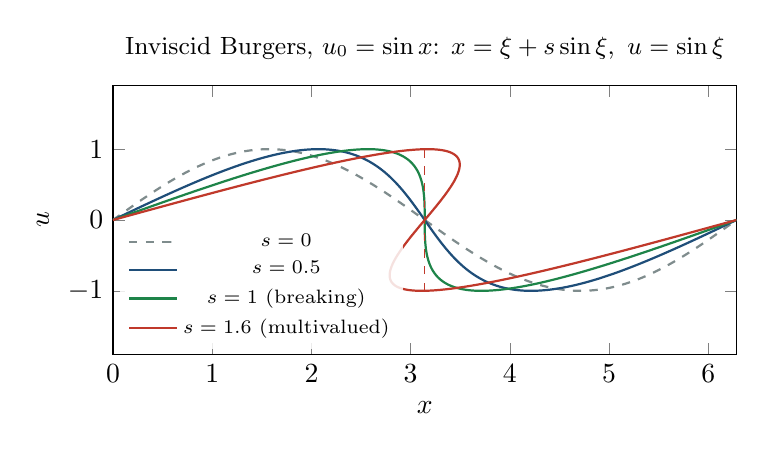
\begin{tikzpicture}
\begin{axis}[width=9.5cm,height=5.0cm,xlabel={$x$},ylabel={$u$},xmin=0,xmax=6.283,ymin=-1.9,ymax=1.9,
 legend style={font=\scriptsize,draw=none,fill=white,fill opacity=0.85,text opacity=1,at={(0.01,0.02)},anchor=south west},
 title={\small Inviscid Burgers, $u_0=\sin x$: $x=\xi+s\sin\xi,\ u=\sin\xi$},no markers,domain=0:6.283185,samples=200,smooth]
\addplot[cG,thick,dashed,variable=\z] ({\z},{sin(deg(\z))});
\addplot[cA,thick,variable=\z] ({\z+0.5*sin(deg(\z))},{sin(deg(\z))});
\addplot[cC,thick,variable=\z] ({\z+1.0*sin(deg(\z))},{sin(deg(\z))});
\addplot[cB,thick,variable=\z] ({\z+1.6*sin(deg(\z))},{sin(deg(\z))});
\draw[cB,dashed] (axis cs:3.14159,-1) -- (axis cs:3.14159,1);
\legend{$s=0$,$s=0.5$,$s=1$ (breaking),$s=1.6$ (multivalued)}
\end{axis}
\end{tikzpicture}
\caption{Characteristic solution of the inviscid flow of $-uu_x$. At $s=1$ the profile has a vertical tangent: the gradient blows up. Beyond that the curve folds; the physical (entropy) solution replaces the fold by a jump at $x=\pi$ (equal-area rule), shown dashed. This breaking is what makes $\Eint$ discontinuous after the shock.}\label{fig:burgers}
\end{figure}
\paragraph{Before the shock ($t<t^*$): smooth regime.} Smoothness permits perturbative expansions and derivative-based estimates.
\begin{itemize}[nosep]
\item $\Eint$ has a closed form at first order in $\nu$, with remainder $O(\nu^2\varepsilon^2t^3)$ \led{S4T-T2} \proved; it blows up at the breaking time $t^*$ \led{S4T-P3}. (This is the same family of expansions as Theorem~\ref{thm:jet} and Example~\ref{ex:burgers-jet}.)
\item The Cole--Hopf substitution $u=-2\nu\varphi_x/\varphi$ turns Burgers into the heat equation $\varphi_t=\nu\varphi_{xx}$; the inverse scattering transform linearizes KdV and NLS. These are used as the ``exact linearization'' of the nonlinear solution~\cite{ch}.
\end{itemize}
\paragraph{At breaking ($t=t^*$): estimates that need smoothness fail.} The inviscid gradient $u_x$ blows up (vertical tangent, $s=1$ in Figure~\ref{fig:burgers}), so every statement that needs bounds on $u_x,u_{xx},\dots$ stops being usable at $t^*$: the closed form of $\Eint$ blows up, and estimates that require smoothness, such as those behind the jet expansion of Theorem~\ref{thm:jet}, are no longer valid.
\paragraph{After the shock ($t>t^*$): discontinuous regime.}
The flow of $-uu_x$ alone forms a shock, so $\Eint$ jumps by amounts independent of $\nu$; this is forced by the definition. A function with a jump is not in $H^1$ in one dimension, so the Sobolev norms of Sections~\ref{sec:groups} and~\ref{sec:inside} are no longer the natural ones: pointwise values are unreliable, while the \emph{measure} of the discrepancy is well behaved. The meaningful quantities are therefore $L^1$ sizes, collected below:
\begin{align}
\|\Eint\|_{L^1}&=\Theta(\nu),\\
\sup_{t\le T}\|\Eint\|_{L^1}&=\nu|\log\nu|+O(\nu),\\
\|S-S_1S_2\|_{L^1}&=\Theta(\sqrt\nu).
\end{align}
The first line holds at fixed $t$, each shock contributing $4\nu\log\!\big(2\cosh(\rho/2)\big)$; the second has exact leading coefficient $1$. Sources: the first line is \led{OPA-T1} \modulo{Kru\v zkov uniqueness~\cite{kr}}; the second is \led{OPF5A-T1/T2}; the third is \led{OPF5D-T6} \proved.
The second line holds for data with a single birth of shock such as $\sin x$, and is conditional on a localization lemma in general \condl{}.

\begin{table}[!htb]
\centering\small
\begin{tabular}{@{}L{3.0cm}L{4.9cm}L{6.2cm}@{}}
\toprule
Regime & What happens & Tools and results\\\midrule
Before the shock, $t<t^*$ & the profile is smooth, characteristics do not cross & jet expansion (Thm.~\ref{thm:jet}), first-order closed form of $\Eint$, Cole--Hopf\\
At breaking, $t=t^*$ & the inviscid gradient blows up (vertical tangent) & smoothness-based estimates fail; $\Eint$ blows up\\
After the shock, $t>t^*$ & the single-term flow is discontinuous (equal-area rule) & $L^1$ estimates: $\Theta(\nu)$, $\nu|\log\nu|$, $\Theta(\sqrt\nu)$\\
\bottomrule
\end{tabular}
\caption{The three regimes of the Burgers interaction term and the tools that apply in each.}\label{tab:regimes}
\end{table}

\subsection{Identification relative to a dictionary}
Nonlinear terms cannot be handled by the ideal $\Ann(u)$ of Section~\ref{sec:theory}; instead one fixes a finite candidate list. Choose a dictionary $\mathcal D$ of monomials of degree $\le d$ in the jet, of order $\le k$, and ask which polynomial relations $F(u,u_x,\dots)=0$ the data satisfy. Notation: $V$ is the span of $\mathcal D$, $I(u)$ the ideal of all differential relations satisfied by $u$, $[F]$ the differential ideal generated by $F$, and $\mathcal J_u$ the jet-level obstruction (a different object from the cofactor $J_u$ of Section~\ref{sec:theory}, hence the calligraphic letter)\edmark{E13}.
\begin{theorem}[{(Dictionary criterion) \led{S4ID-T1} \proved[]}]\label{thm:dict}
For smooth $u$ on any $\Omega$ there is an exact sequence $0\to[F]\cap V\to I(u)\cap V\to\mathcal J_u\cap\psi(V)\to0$. In particular
\[
I(u)\cap V=[F]\cap V\iff\mathcal J_u\cap\psi(V)=0 .
\]
\end{theorem}
The correct statement is therefore ``the relations are exactly $F$ \emph{modulo its differential consequences}''; the literal ``$I(u)\cap V=\langle F\rangle$'' is false in complete dictionaries (they contain $\partial_xF$, etc.) \led{S4ID-P1}. Concrete criteria: for Burgers with $N$ shocks, $u$ identifies the equation in the evolutionary dictionary iff $d\le N$ \led{S4ID-T2, OP-T7}; for $N$-soliton KdV the identifying polynomial has total degree $(N+2)2^{N-1}$ (generic $N=2$: $8$) \led{OP-K15} \modulo{Novikov 1974~\cite{no}}. Finally, ``closed form $\Rightarrow$ does not identify'' is itself a theorem \led{S4ID-T4}.
\edmark{E2}

\subsection{Linear versus nonlinear: the same idea, two structures}
Sections~\ref{sec:theory}--\ref{sec:inside} and the present one answer the same question: \emph{what does a single solution $u$ remember about its equation?} In both settings we collect all relations satisfied by $u$ and ask when these relations are generated by the equation we were given. What changes is the algebraic structure in which the relations live.
\begin{table}[!htb]
\centering\small
\begin{tabular}{@{}L{2.8cm}L{6.2cm}L{6.2cm}@{}}
\toprule
 & Linear approach (Sections~\ref{sec:theory}--\ref{sec:inside}) & Nonlinear approach (this section)\\\midrule
Space of candidate equations & the ring $\ring=\C[\tau,\xi]$ of constant-coefficient operators & a finite \emph{dictionary} $\mathcal D$ of jet monomials of degree $\le d$ and order $\le k$; $V=\spn\mathcal D$\\
Relations satisfied by $u$ & $\Ann(u)$, an ideal of $\ring$ & $I(u)$, the ideal of all differential relations\\
What the equation generates & the principal ideal $(P)$ & the differential ideal $[F]$\\
Criterion for identification & $\Ann(u)=(P)$ (Theorem~\ref{thm:ident}) & $I(u)\cap V=[F]\cap V$, i.e.\ $F$ \emph{modulo its differential consequences} (Theorem~\ref{thm:dict})\\
What escapes the equation & the cofactor $J_u$: the finitely many exponentials in $u$ ($\sigma_p(u)=\Var(J_u)$) & the jet-level obstruction $\mathcal J_u\cap\psi(V)$ (exact sequence of Theorem~\ref{thm:dict})\\
Solutions that do not identify & $u\in\EP$ & closed-form solutions (\led{S4ID-T4})\\
Concrete criteria & finite linear algebra (Lemma~\ref{lem:ep}) & Burgers with $N$ shocks identifies iff $d\le N$; $N$-soliton KdV: degree $(N+2)2^{N-1}$\\
\bottomrule
\end{tabular}
\caption{The linear and nonlinear identification problems side by side.}\label{tab:lin-nonlin}
\end{table}
\begin{aside}{Where the parallel breaks}
\textbf{Linear case.} The solutions form a vector space and the annihilators an ideal: one can add, multiply by operators and factor, which is why the Nullstellensatz applies and the test is a finite-dimensional computation.

\textbf{Nonlinear case.} There is no linear structure on the solutions: one must fix a finite space $V$ of candidates in advance, and the identification is \emph{relative to $V$}, never absolute. The literal statement
\[
I(u)\cap V=\langle F\rangle
\]
is false in complete dictionaries, which contain $\partial_xF$, so the correct statement is ``modulo differential consequences''.
\end{aside}

\begin{keypoint}
Both approaches ask what one solution determines about its equation. The linear one answers with the annihilator ideal $\Ann(u)$ and its generator $G_u$; the nonlinear one answers with a dictionary and the differential ideal of relations, and only up to differential consequences. In the algorithm of the companion paper Steps~1--6 use the structure of $\Ann(u)$, while Step~7 switches to the dictionary and returns a relative identification.
\end{keypoint}

%======================================================================

% ---- end sections/port_nonlinear.tex


\section*{Part I-B: the full development of Phases 0--5}
\addcontentsline{toc}{section}{Part I-B: the full development of Phases 0--5}
\noindent The sections above give the main line of Phases 0--5 in the order of the grouping principle. The following sections are the full-length chapters of the complete edition (abstract and reading guide, overview, algebra primer, the algebraic language, identification, finite data and decidability,
decomposition, regularity, the interaction term, nonlinear equations, the algorithm, limits, and the open problems and directions of Phases 0--5), with every theorem, example and warning; labels that coincide with those above are prefixed by \texttt{f:} in the source. Proofs are cited as ``Dim.~An/Bn'' in the companion proofs file.

% ---- begin sections/full_front.tex
\section*{Abstract of the complete edition}
\addcontentsline{toc}{section}{Abstract}

We are given one exact solution $u(t,x)$ of a differential equation that we do not know. What does $u$ remember about its equation? This edition answers the question for the results of Phases~0--10 of the project. The answer has four parts for constant coefficients (Part~I) and four more for what lies beyond (Part~II).

\textbf{Identification.} For constant coefficients, $u$ determines its operator $P$ exactly when no partial quotient
\[
w_i=\Big(\frac{P}{P_i}\Big)(\partial)\,u
\]
is an exponential-polynomial. No finite amount of data can certify this, and a black-box test is impossible. One extra integer, a bound on the exponential-polynomial part of $u$, makes it a finite computation.

\textbf{Decomposition.} On a simply connected region, $u$ splits into one component per irreducible \emph{factor} of the symbol. The ambiguity has the exact finite dimension $\delta(P)$. The split per additive \emph{term} of the operator is false. The components keep the Sobolev regularity of $u$ exactly when a conditioning number $\gamma_N$ is positive.

\textbf{Interaction.} For an evolution equation whose $N$ terms commute, the part of the solution due to the interplay of the terms is
\[
\Eint=\Big[\prod_{n=1}^N(\Id+\Delta_n)-\Id-\sum_{n=1}^N\Delta_n\Big]u_0 .
\]
One value costs $O(N)$ operations, while the full table of cross terms costs $\Theta(2^N)$. The map $u_0\mapsto\Eint$ is not continuous in Sobolev norms and cannot be regularised.

\textbf{Nonlinear equations.} For Burgers, KdV--Burgers and KdV the same questions have sharp answers. The interaction has a $t^2$ jet and a closed form before the shock, and size $\Theta(\nu)$ and $\nu|\log\nu|$ after it. Identification holds relative to a dictionary, modulo the differential consequences of the equation. For the $N$-soliton of KdV the identifying polynomial has degree $(N+2)2^{N-1}$.

\textbf{Beyond constant coefficients (Part~II).} \emph{Systems:} a vector solution determines a matrix operator iff every socle of its module has dimension at most one, which holds for every non-singular square system in two or more variables; gauge can never be separated from physics by one field. \emph{Variable coefficients:} a potential $V(x)$ is read from any non-zero solution, a potential $V(t,x)$ can hide in silent time strips, and a huge coefficient class identifies nothing. \emph{Convergence and noise:} identification holds in the limit without a certificate, no learner decides whether a law exists, and noise is handled only at a finite level of the dictionary. \emph{The encoder and the dictionary:} an explicit Volterra transformation removes a known potential; a universal dictionary exists for approximation but never for exact identification, and a misfit has a finite certificate while a fit never does. Phase~10 corrected several statements of Phases~1--3: a continuity no-go that was false as stated, and the failure of density on regions with holes.

\subsection*{How to read this edition}

\textbf{Layout.} Every chapter opens with a box with three entries. \emph{Starting from} lists the assumptions in force. \emph{Why} says what problem the chapter solves. \emph{Role} says where its output is used. Inside a chapter the order is always the same: motivation, then intuition, then statement, then a worked example, then consequences.

\textbf{Boxes.} The colours are fixed:
\begin{itemize}
\item blue boxes are theorems, propositions and lemmas;
\item green boxes are definitions;
\item violet bars are worked examples;
\item amber boxes give the intuition;
\item red boxes are warnings and counterexamples.
\end{itemize}

\textbf{Proofs.} Proofs are not in this volume. Each statement names its proof in the companion \emph{Catalogue of proofs}, for example \textsf{\footnotesize\color{cA}Dim.~A3}. Parts~I and~II of the catalogue contain the load-bearing proofs of Phases~0--5 (A1--A31) and of Phases~6--10 (A32--A53); Parts~III and~IV contain all the others.

\textbf{Trust labels.} Every statement carries one label. \proved{} means a complete proof that passed an independent review. \modulo{X} means complete except for a cited published theorem~X whose source was checked. \pw{} means a full proof exists but no independent audit has been done. \cf{} means a published theorem we rely on. \condl{} means the result depends on an unverified lemma. \vex{} means it was only checked on examples. \openq{} means unsolved. \falsest{} means a counterexample is proved. The reviewers were independent AI agents, not human referees. Grey tags such as \led{C3-T1} are the identifiers in the project ledger \texttt{claims/LEDGER.md}.

\textbf{Prerequisites.} Linear algebra (eigenvalues, Jordan form), calculus in two variables, the Fourier transform, and linear ODEs with constant coefficients. Chapter~\ref{ch:primer} introduces every algebraic notion from scratch: ideals, annihilators, exponential-polynomials and the Chinese remainder theorem.

\textbf{Scope.} This edition covers Phases~0--10; a separate pair of volumes covers Phases~0--5 alone. In case of a difference the present edition prevails. 


% ---- end sections/full_front.tex


% ---- begin sections/full_ch1.tex
\section{Overview of the full development}\label{ch:intro}
\sectionbrief
{one function $u(t,x)$, known exactly (no noise) on an open region $\Omega\subset\R^2$, which solves a linear equation $P(\partial_t,\partial_x)u=0$ with constant coefficients. The operator $P$ is \emph{not} given.}
{to state precisely what we want to learn from $u$ and to give a map of the answers before any detail.}
{frames the three questions Q1--Q3. Sections~\ref{f:ch:ident}--\ref{f:ch:data} answer Q1, Sections~\ref{f:ch:decomp}--\ref{f:ch:regular} answer Q2, Section~\ref{f:ch:interaction} answers Q3. Section~\ref{f:ch:nonlin} extends all three to nonlinear equations and Section~\ref{ch:algo} assembles them into an algorithm. Part~II (Sections~\ref{ch:systems}--\ref{f:ch:status}) goes beyond constant coefficients and states the limits of the whole project.}

\subsection{The question}

Suppose we observe a physical field $u(t,x)$: a temperature, a wave, a concentration. We know $u$ exactly on some region $\Omega$ of the $(t,x)$ plane, and we know that it obeys some linear law. We do not know which law. Three questions arise naturally.

\begin{enumerate}[label=\textbf{Q\arabic*.},leftmargin=1.2cm]
\item \textbf{Identification.} Can the operator $P$ be reconstructed from $u$? When is the answer unique?
\item \textbf{Decomposition.} If $P$ is built from pieces, can $u$ be split into the parts that each piece generates?
\item \textbf{Interaction.} If the pieces are the \emph{terms} of the operator (diffusion, advection, dispersion, \dots), which part of $u$ is due to no single term but to their interplay? Can it be computed exactly and cheaply?
\end{enumerate}

The setting is deliberately analytic. There is no statistical model, no learned weights and no noise. The aim is an \emph{exact} procedure, together with a precise statement of what is impossible.

\begin{example}[{Three solutions of the heat equation}]
Take the heat equation $u_t=Du_{xx}$ with $D>0$. Consider three of its solutions.
\begin{itemize}
\item A single Fourier mode:
\[
u_1=e^{-D\kappa^2t}\cos(\kappa x).
\]
\item A sum of two modes:
\[
u_2=e^{-Dt}\cos x+e^{-4Dt}\cos 2x.
\]
\item The heat kernel, for $t>0$:
\[
u_3=\frac{1}{\sqrt{t}}\;e^{-x^2/(4Dt)}.
\]
\end{itemize}
All three solve the same equation. We will see that only $u_3$ determines it. The function $u_1$ also solves $u_{xx}=-\kappa^2u$ and $u_t=-D\kappa^2u$, and from $u_1$ alone we cannot tell which of these laws is ``the'' law. The difference is that $u_1$ and $u_2$ are finite sums of exponentials, while $u_3$ is not (Section~\ref{f:ch:ident}, Example~\ref{ex:heat3}).
\end{example}

\subsection{Overview of the answers}

Figure~\ref{fig:pipeline} shows the logical chain, read from left to right. Each box is a task. Each arrow is a theorem that allows the next task to be carried out, under its own hypotheses.

\begin{figure}[!htb]
\centering
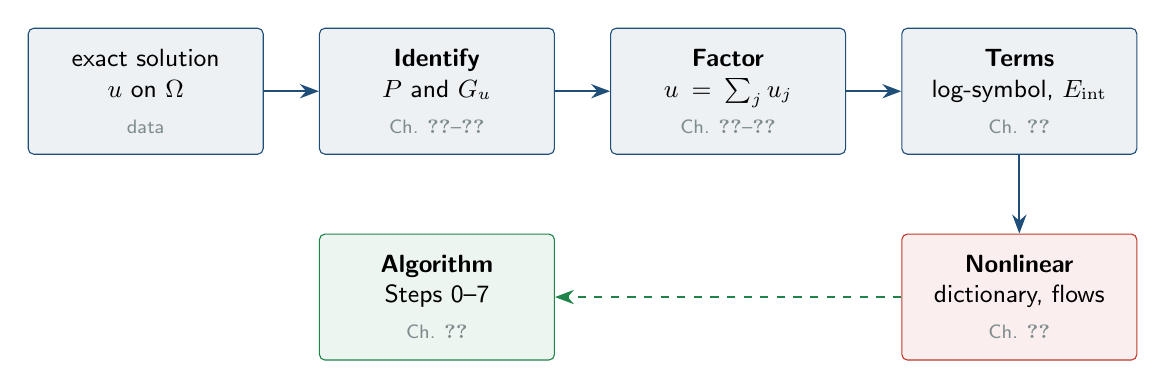
\begin{tikzpicture}[node distance=7mm,
  box/.style={draw=cA,fill=cA!8,rounded corners=2pt,minimum height=16mm,text width=2.75cm,align=center,font=\small\sffamily},
  arr/.style={-{Stealth[length=2.4mm]},thick,cA}]
\node[box] (u) {exact solution\\$u$ on $\Omega$\\[2pt]{\scriptsize\textcolor{cG}{data}}};
\node[box,right=of u] (id) {\textbf{Identify}\\ $P$ and $G_u$\\[2pt]{\scriptsize\textcolor{cG}{Ch.~\ref{f:ch:ident}--\ref{f:ch:data}}}};
\node[box,right=of id] (fa) {\textbf{Factor}\\ $u=\sum_ju_j$\\[2pt]{\scriptsize\textcolor{cG}{Ch.~\ref{f:ch:decomp}--\ref{f:ch:regular}}}};
\node[box,right=of fa] (te) {\textbf{Terms}\\ log-symbol, $\Eint$\\[2pt]{\scriptsize\textcolor{cG}{Ch.~\ref{f:ch:interaction}}}};
\node[box,below=10mm of te,fill=cB!8,draw=cB] (nl) {\textbf{Nonlinear}\\ dictionary, flows\\[2pt]{\scriptsize\textcolor{cG}{Ch.~\ref{f:ch:nonlin}}}};
\node[box,below=10mm of id,fill=cC!8,draw=cC] (al) {\textbf{Algorithm}\\ Steps 0--7\\[2pt]{\scriptsize\textcolor{cG}{Ch.~\ref{ch:algo}}}};
\draw[arr] (u)--(id); \draw[arr] (id)--(fa); \draw[arr] (fa)--(te); \draw[arr] (te)--(nl);
\draw[arr,cC,dashed] (nl)--(al);
\end{tikzpicture}
\caption{Logical structure of the method. The three linear stages (blue) are followed by the nonlinear extension (red). The algorithm (green) chains all of them. A step can only be trusted under the hypotheses of the theorem that precedes it.}\label{fig:pipeline}
\end{figure}

Table~\ref{f:tab:results} lists the main statements with their status. Every row points to the chapter where the statement is made precise.

\begin{table}[!htb]
\centering\small
\begin{tabular}{@{}L{2.8cm}L{8.6cm}L{3.0cm}@{}}
\toprule
Topic & Result & Status\\\midrule
Identification & $\Ann(u)=(P)$ iff no $w_i=(P/P_i)(\partial)u$ is an exponential-polynomial (Ch.~\ref{f:ch:ident}) & \proved\\
Spectral form & $\Ann(u)=(P)$ iff the point spectrum is empty and $G_u\sim P$ (Ch.~\ref{f:ch:ident}) & \proved\\
Finite data & a jet of order $2d-1$ suffices for exponential-polynomials; no finite certificate otherwise; black box impossible; decidable with a bound (Ch.~\ref{f:ch:data}) & \proved\\
Decomposition & $\ker P=\sum_j\ker Q_j$ on simply connected $\Omega$, ambiguity $\delta(P)$ (Ch.~\ref{f:ch:decomp}) & \proved\\
Terms & splitting per additive term is false (Ch.~\ref{f:ch:decomp}) & \proved\\
Regularity & components in $H^m$ iff the sum of kernels is closed ($\gamma_N>0$) and dense (Ch.~\ref{f:ch:regular}) & \proved\\
Interaction & closed product formula; $O(N)$ per value, $\Theta(2^N)$ per table (Ch.~\ref{f:ch:interaction}) & \proved\\
Stability & $u_0\mapsto\Eint$ is not continuous in $H^m$; no stable regularisation (Ch.~\ref{f:ch:interaction}) & \proved\\
Nonlinear & Burgers: jet, closed form before the shock, $\Theta(\nu)$ and $\nu|\log\nu|$ after (Ch.~\ref{f:ch:nonlin}) & \proved{} / \modulo{Kru\v zkov}\\
Dictionary & identification modulo differential consequences; KdV degree $(N+2)2^{N-1}$ (Ch.~\ref{f:ch:nonlin}) & \proved{} / \modulo{Novikov}\\\bottomrule
\end{tabular}
\caption{Main results, in the order in which they appear.}\label{f:tab:results}
\end{table}

\subsection{Notation at a glance}

Table~\ref{tab:notation} collects the symbols used throughout, with the place where each one is defined. Some letters have different meanings in different chapters; the caption lists them.

\begin{table}[!htb]
\centering\small
\begin{tabular}{@{}L{3.1cm}L{8.9cm}L{2.5cm}@{}}
\toprule
Symbol & Meaning & Defined in\\\midrule
$(t,x)$, $\Omega$ & time and space; the open region where $u$ is known & Ch.~\ref{ch:intro}\\
$\partial=(\partial_t,\partial_x)$ & partial derivatives & Ch.~\ref{f:ch:algebra}\\
$\ring=\C[\tau,\xi]$ & ring of constant-coefficient operators, $\tau\leftrightarrow\partial_t$, $\xi\leftrightarrow\partial_x$ & Def.~\ref{f:def:ring}\\
$P$, $P_i$, $e_i$ & the operator (its symbol), its irreducible factors, their multiplicities & Ch.~\ref{f:ch:algebra}\\
$Q_j=P_j^{m_j}$ & pairwise coprime factors used for decomposition & Ch.~\ref{f:ch:decomp}\\
$\Var(P)$ & characteristic variety: zeros of the symbol in $\C^2$ & Def.~\ref{f:def:ring}\\
$\Ann(u)$ & the ideal of all operators that annihilate $u$ & Def.~\ref{f:def:ann}\\
$G_u$, $J_u$ & $G_u=\Gcd\Ann(u)$ and the cofactor ideal: $\Ann(u)=G_u\,J_u$ & Lemma~\ref{f:lem:gcd}\\
$\EP$ & exponential-polynomials & Def.~\ref{f:def:ep}\\
$\sigma_p(u)$ & point spectrum $\Var(J_u)$ & Ch.~\ref{f:ch:ident}\\
$\delta(P)$ & dimension of the ambiguity of the factor decomposition & Ch.~\ref{f:ch:decomp}\\
$c_F$, $\gamma_N$ & Friedrichs cosine; conditioning number of the sum map & Ch.~\ref{f:ch:regular}\\
$A_n$, $S_n(t)$, $\Delta_n$ & terms of an evolution, their flows, increments $S_n-\Id$ & Ch.~\ref{f:ch:interaction}\\
$\Eint$ & interaction term & Eq.~\eqref{f:eq:eint-def}\\
$T_n$, $V$, $I(u)$ & nonlinear terms; dictionary span; ideal of relations of $u$ & Ch.~\ref{f:ch:nonlin}\\
\bottomrule
\end{tabular}
\caption{Notation guide. Overloaded letters: $S$ is a flow in Section~\ref{f:ch:interaction} and the sum map in Section~\ref{f:ch:regular}; $D$ is $d/dx$ in Section~\ref{sec:ode} and a diffusion constant elsewhere; $J$ denotes ideals.}\label{tab:notation}
\end{table}

\subsection{Roadmap}

The chapters build on each other in the following order.
\begin{itemize}
\item \textbf{Section~\ref{ch:primer}} is a primer. It explains ideals, annihilators, exponential-polynomials, the Chinese remainder theorem and the companion matrix, starting from integers and one-variable ODEs. A reader who already knows these notions can skip it.
\item \textbf{Section~\ref{f:ch:algebra}} fixes the algebraic language: symbols, the annihilator ideal, its gcd splitting and the finite-dimension test for exponential-polynomials. It ends with the one-variable prototype.
\item \textbf{Sections~\ref{f:ch:ident} and~\ref{f:ch:data}} answer Q1. The first gives the exact criterion and the intrinsic operator $G_u$. The second asks what can be decided from finite data.
\item \textbf{Sections~\ref{f:ch:decomp} and~\ref{f:ch:regular}} answer Q2. The first proves the factor decomposition and shows why splitting by terms fails. The second asks when the pieces keep the regularity of $u$.
\item \textbf{Section~\ref{f:ch:interaction}} answers Q3: the exact interaction term, its cost, and its instability.
\item \textbf{Section~\ref{f:ch:nonlin}} extends the three questions to nonlinear equations.
\item \textbf{Section~\ref{ch:algo}} turns the theorems into an algorithm with two fully worked examples.
\item \textbf{Sections~\ref{ch:systems}--\ref{ch:dictionary}} (Part~II) go beyond constant coefficients: systems and gauge, variable coefficients, convergence and noise, the analytic encoder, and the universal dictionary.
\item \textbf{Section~\ref{ch:phase10}} records what Phase~10 changed in the statements of the earlier phases.
\item \textbf{Section~\ref{ch:extalgo}} extends the algorithm to all of the above, with a contract for every step.
\item \textbf{Section~\ref{f:ch:status}} states what is impossible, what is open, and how reliable each result is, for the whole project.
\end{itemize}


% ---- end sections/full_ch1.tex


% ---- begin sections/full_ch2.tex
\section{A primer for readers new to the algebra}\label{ch:primer}
\sectionbrief
{only linear algebra, polynomials and linear ODEs with constant coefficients.}
{the whole theory speaks the language of rings and ideals. Every notion used later is introduced here from a familiar starting point: integers first, then ODEs in one variable, then two variables.}
{nothing later depends on reading this chapter, but every later chapter uses its vocabulary. It covers ideals and annihilators (\S\ref{sec:pr-ideal}), exponential-polynomials (\S\ref{sec:pr-ep}), the Chinese remainder theorem (\S\ref{sec:pr-crt}) and the companion matrix (\S\ref{sec:pr-comp}).}

\subsection{Ideals and annihilators, starting from integers}\label{sec:pr-ideal}

\subsubsection{Integers}

The multiples of $6$ form the set
\[
(6)=\{\dots,-12,-6,0,6,12,\dots\}.
\]
This set has two properties. The sum of two multiples of $6$ is a multiple of $6$. A multiple of $6$ times any integer is again a multiple of $6$. A subset of a ring with these two properties is called an \emph{ideal}.

Now take the ideal generated by $4$ and $6$, that is, all combinations $4a+6b$ with integers $a,b$:
\[
(4,6)=\{4a+6b:\ a,b\in\Z\}.
\]
Since $2=6-4$ lies in it, and every element is even, we get $(4,6)=(2)$. The ideal ``remembers'' only the greatest common divisor of its generators. In $\Z$ every ideal is generated by one number.

\subsubsection{Operators in one variable}

Replace integers by differential operators with constant coefficients in one variable $x$, and replace ``is a multiple of $6$'' by ``kills the function $u$''.

\begin{definition}[{Annihilator (one variable)}]
For a function $u(x)$, the annihilator of $u$ is the set of all polynomials $Q$ such that the operator $Q(d/dx)$ kills $u$:
\[
\Ann(u)=\Big\{Q\in\C[\xi]:\ Q\Big(\frac{d}{dx}\Big)u=0\Big\}.
\]
\end{definition}

It is an ideal. If $Q$ kills $u$ and $S$ is any polynomial, then $SQ$ kills $u$ too, because $S(d/dx)$ applied to $0$ is $0$. Sums of annihilators are annihilators.

\begin{example}[{Annihilators of familiar functions}]
Write $\partial=d/dx$. The operator $\partial-1$ kills $e^x$, and so does every multiple of it. The basic cases are:
\begin{align*}
\Ann(e^x)&=(\partial-1),\\
\Ann(\sin x)&=(\partial^2+1),\\
\Ann(xe^x)&=\big((\partial-1)^2\big),\\
\Ann(e^x+e^{2x})&=\big((\partial-1)(\partial-2)\big).
\end{align*}
The function $e^{x^2}$ has annihilator $\{0\}$: no nonzero polynomial in $\partial$ kills it, because each derivative $\partial^ke^{x^2}$ equals a polynomial of degree exactly $k$ times $e^{x^2}$.
\end{example}

In one variable every ideal has a single generator, exactly as in $\Z$. The generator of $\Ann(u)$ is the \emph{minimal annihilator} of $u$: the ODE of lowest order that $u$ satisfies.

\subsubsection{Two variables: the new feature}

With two variables $t$ and $x$ we have two derivatives. An operator is a polynomial in both. Here an ideal may need \emph{several} generators.

\begin{example}[{An ideal with two generators}]
Let $u=e^{2t+3x}$. Then
\[
(\partial_t-2)u=0\qquad\text{and}\qquad(\partial_x-3)u=0 .
\]
Every operator of the form $A\,(\partial_t-2)+B\,(\partial_x-3)$ kills $u$, and these are all of them. So
\[
\Ann(u)=(\partial_t-2,\ \partial_x-3).
\]
No single polynomial generates this ideal: a polynomial in the ideal vanishes at the point $(2,3)$, and a single polynomial vanishes on a whole curve, not at a single point.
\end{example}

This is the source of every subtlety in the theory. A solution of a PDE has an annihilator that may contain a ``curve part'' (one polynomial) and a ``point part'' (finitely many points). Lemma~\ref{f:lem:gcd} of the next chapter makes this precise.

\subsection{Exponential-polynomials}\label{sec:pr-ep}

An \emph{exponential-polynomial} is a finite sum of polynomials times exponentials:
\[
w(t,x)=\sum_{j=1}^{r}p_j(t,x)\,e^{\tau_jt+\xi_jx}.
\]
These are exactly the solutions of ODEs with constant coefficients, in each variable. They are the ``trivial'' solutions of the theory: they live on finitely many points of the characteristic variety.

The key property is a finite-dimension test. Differentiate $w$ as often as you like: you always stay inside a finite-dimensional space.

\begin{example}[{Which functions are exponential-polynomials?}]
\begin{center}\small
\begin{tabular}{@{}L{4.4cm}L{1.6cm}L{8.0cm}@{}}
\toprule
Function & In $\EP$? & Span of all derivatives\\\midrule
$xe^{x}$ & yes & $\spn\{xe^x,\ e^x\}$, dimension $2$\\
$x^2e^{3t}+\cos x$ & yes & finite: $\cos x=\tfrac12(e^{ix}+e^{-ix})$\\
$e^{-x^2}$ & no & $\partial_x^ke^{-x^2}=(\text{degree }k)\cdot e^{-x^2}$: infinite dimension\\
$1/(1+x^2)$ & no & denominators $(1+x^2)^{k+1}$ grow: infinite dimension\\
$f(x+t)$, $f$ a Gaussian & no & same as the Gaussian\\
\bottomrule
\end{tabular}
\end{center}
The test ``is the span of the derivatives finite-dimensional?'' is Lemma~\ref{f:lem:ep}.
\end{example}

\subsection{The Chinese remainder theorem}\label{sec:pr-crt}

\subsubsection{Integers}

Solve the system
\[
x\equiv1\pmod 2,\qquad x\equiv2\pmod 3 .
\]
The unique solution modulo $6$ is $x\equiv5$. In general, if $a$ and $b$ are coprime, a remainder modulo $a$ and a remainder modulo $b$ determine a unique remainder modulo $ab$. In the language of rings:
\[
\Z/(ab)\;\cong\;\Z/(a)\times\Z/(b).
\]

\subsubsection{ODEs in one variable}

Let $p(\partial)=(\partial-1)(\partial-2)$. Its solutions are $u=ae^x+be^{2x}$. The two pieces can be extracted by \emph{projector operators}:
\begin{align*}
u_1&=\frac{\partial-2}{1-2}\,u=a\,e^{x},\\[3pt]
u_2&=\frac{\partial-1}{2-1}\,u=b\,e^{2x}.
\end{align*}
Check the first line: $(\partial-2)(ae^x+be^{2x})=-ae^x$, and dividing by $1-2=-1$ gives $ae^x$. The sum is direct:
\[
\ker p(\partial)=\ker(\partial-1)\oplus\ker(\partial-2).
\]
This works because $\partial-1$ and $\partial-2$ are coprime: there are polynomials $a,b$ with $a(\partial-1)+b(\partial-2)=1$ (here $a=1$, $b=-1$).

\subsubsection{Two variables: what changes}

For the wave operator $P=\tau^2-\xi^2=(\tau-\xi)(\tau+\xi)$ the two factors are coprime, but no combination of them equals $1$. Indeed
\[
(\tau-\xi,\ \tau+\xi)=(\tau,\ \xi),
\]
the ideal of the single point $(0,0)$ where the two lines meet. The quotient
\[
\ring/(\tau,\xi)\cong\C
\]
has dimension $1$. This number is the ambiguity of the splitting: the d'Alembert components $f(x+t)$ and $g(x-t)$ are defined only up to a constant moved from one to the other. Theorem~\ref{f:thm:factor} says that this finite overlap is the \emph{only} failure of the integer picture.

\subsection{The companion matrix}\label{sec:pr-comp}

A linear ODE of order $m$ becomes a first-order system for the vector of derivatives. For
\[
u''-3u'+2u=0
\]
put $X=(u,u')^{\top}$. Then $X'=CX$ with
\[
C=\begin{pmatrix}0&1\\-2&3\end{pmatrix}.
\]
The characteristic polynomial of $C$ is $\lambda^2-3\lambda+2$, the symbol of the ODE, with roots $1$ and $2$. The Lagrange projectors are
\[
\Pi_1=\frac{C-2\,\Id}{1-2},\qquad \Pi_2=\frac{C-\Id}{2-1},
\]
and the matrix exponential splits into modes:
\[
e^{xC}=e^{x}\,\Pi_1+e^{2x}\,\Pi_2 .
\]
This is the same formula as the projectors of the previous section, written for matrices. It reappears as the Lagrange formula~\eqref{f:eq:lagrange} for evolution factors.

\begin{keypoint}
Four ideas carry the theory. An \emph{ideal} records all equations a function satisfies. Its \emph{gcd} separates a curve part from finitely many points. \emph{Exponential-polynomials} are the functions with finitely many derivatives up to linear dependence. The \emph{Chinese remainder theorem} splits a solution into pieces, up to a finite overlap.
\end{keypoint}


% ---- end sections/full_ch2.tex


% ---- begin sections/full_ch3.tex
\section{The algebraic language}\label{f:ch:algebra}
\sectionbrief
{constant coefficients; functions or distributions on $\Omega\subset\R^2$ with complex values. The vocabulary of Section~\ref{ch:primer}.}
{three notions carry the whole theory. The \emph{symbol} turns derivatives into polynomials. The \emph{annihilator} collects all equations a function satisfies. \emph{Exponential-polynomials} are the trivial solutions.}
{foundation for every later chapter. It proves the two lemmas that every identification argument uses (Lemmas~\ref{f:lem:gcd} and~\ref{f:lem:ep}) and ends with the one-variable prototype (Section~\ref{sec:ode}).}

\subsection{Derivatives as polynomials}

A linear operator with constant coefficients is a polynomial in the two partial derivatives:
\[
P(\partial_t,\partial_x)=\sum_{j,k}c_{jk}\,\partial_t^{\,j}\,\partial_x^{\,k},\qquad c_{jk}\in\C .
\]
The exponentials are eigenfunctions of every derivative. Write
\[
e_{\tau,\xi}(t,x)=e^{\tau t+\xi x}.
\]
Then
\[
\partial_t\,e_{\tau,\xi}=\tau\,e_{\tau,\xi},\qquad
\partial_x\,e_{\tau,\xi}=\xi\,e_{\tau,\xi},
\]
and therefore, for every operator $P$,
\begin{equation}\label{eq:symbol}
P(\partial)\,e_{\tau,\xi}=P(\tau,\xi)\,e_{\tau,\xi}.
\end{equation}
So applying the operator to an exponential is the same as multiplying by the value of a polynomial. This is the reason why all the algebra below is about polynomials in two variables.

\begin{definition}[{Operator ring, symbol, characteristic variety}]\label{f:def:ring}
The ring of constant-coefficient operators is
\[
\ring=\C[\partial_t,\partial_x]\;\cong\;\C[\tau,\xi].
\]
The polynomial $P(\tau,\xi)$ is the \emph{symbol} of $P(\partial)$. The \emph{characteristic variety} of $P$ is its zero set
\[
\Var(P)=\{(\tau,\xi)\in\C^2:\ P(\tau,\xi)=0\}.
\]
\end{definition}

By~\eqref{eq:symbol}, the exponential $e_{\tau,\xi}$ solves $P(\partial)u=0$ exactly when $(\tau,\xi)$ lies on $\Var(P)$. Fourier modes are the special case $\xi=i\kappa$ with real frequency $\kappa$.

\begin{figure}[!htb]
\centering
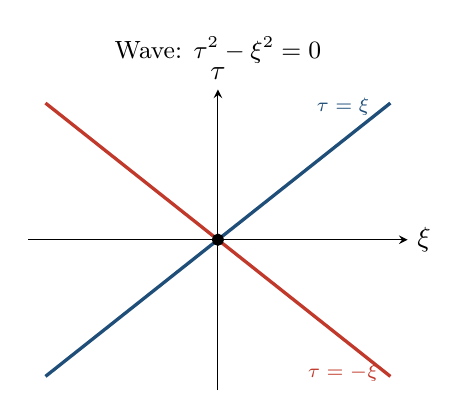
\begin{tikzpicture}
\begin{axis}[width=6.4cm,height=5.4cm,axis lines=middle,xlabel={$\xi$},ylabel={$\tau$},xmin=-2.2,xmax=2.2,ymin=-2.2,ymax=2.2,
 ticks=none,title={\small Wave: $\tau^2-\xi^2=0$},every axis x label/.style={at={(current axis.right of origin)},anchor=west},
 every axis y label/.style={at={(current axis.above origin)},anchor=south}]
\addplot[cA,very thick,domain=-2:2] {x}; \addplot[cB,very thick,domain=-2:2] {-x};
\node[cA,font=\scriptsize] at (axis cs:1.45,1.95) {$\tau=\xi$}; \node[cB,font=\scriptsize] at (axis cs:1.45,-1.95) {$\tau=-\xi$};
\addplot[only marks,mark=*] coordinates {(0,0)};
\end{axis}
\end{tikzpicture}\hfill
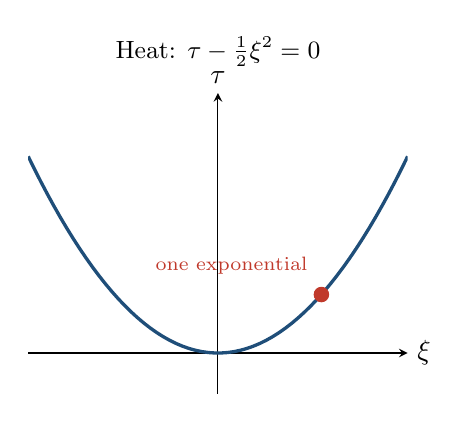
\begin{tikzpicture}
\begin{axis}[width=6.4cm,height=5.4cm,axis lines=middle,xlabel={$\xi$},ylabel={$\tau$},xmin=-2.2,xmax=2.2,ymin=-0.5,ymax=3.2,
 ticks=none,title={\small Heat: $\tau-\tfrac12\xi^2=0$},every axis x label/.style={at={(current axis.right of origin)},anchor=west},
 every axis y label/.style={at={(current axis.above origin)},anchor=south}]
\addplot[cA,very thick,domain=-2.2:2.2,samples=60] {0.5*x^2};
\addplot[only marks,mark=*,cB,mark size=2.6pt] coordinates {(1.2,0.72)};
\node[cB,font=\scriptsize,anchor=south east] at (axis cs:1.15,0.85) {one exponential};
\end{axis}
\end{tikzpicture}
\caption{Real slices of two characteristic varieties. A single exponential solution is a single point of the variety. A rich, non-exponential solution ``fills'' the whole curve.}\label{fig:varieties}
\end{figure}

\subsection{Annihilators and what a solution knows}

A single function is usually killed by many operators. For example, $e^x$ is killed by $\partial_x-1$, by $\partial_x^2-1$, by $\partial_t$, and by every combination of these.

\begin{definition}[{Annihilator}]\label{f:def:ann}
The annihilator of $u$ is the set of all operators that kill $u$:
\[
\Ann(u)=\{Q\in\ring:\ Q(\partial)u=0\}.
\]
\end{definition}

$\Ann(u)$ is an ideal of $\ring$: if $Q(\partial)u=0$ and $S\in\ring$, then
\[
(SQ)(\partial)u=S(\partial)\big(Q(\partial)u\big)=0 ,
\]
and the sum of two annihilators is an annihilator. Three classical facts about $\C[\tau,\xi]$ are used throughout.

\begin{notebox}{Three facts about polynomials in two variables}
\textbf{(F1) Unique factorisation.} Every nonzero polynomial factors as
\[
P=c\prod_iP_i^{e_i},
\]
with $P_i$ irreducible and pairwise non-proportional (the ``primes''), $e_i\ge1$ their multiplicities, and $c$ a constant. The factorisation is unique up to constants, so $\Gcd$ is defined as for integers.

\textbf{(F2) B\'ezout.} Two polynomials without a common factor have only finitely many common zeros, at most the product of their degrees. Geometrically: two curves without a common component meet in isolated points.

\textbf{(F3) Nullstellensatz} (Hilbert). If a polynomial $q$ vanishes on the common zero set $\Var(I)$ of an ideal $I$, then $q^k\in I$ for some $k\ge1$. In particular, an ideal without common zeros is the whole ring.
\end{notebox}

All three are classical~\cite{clo,fu}. They hold over $\C$; the Nullstellensatz fails over $\R$.

The next lemma says that every ideal splits into a ``curve part'' (one polynomial) and a residue that vanishes only at finitely many points.

\begin{lemma}[{Splitting off the gcd \led{C3-L2} \proved}]\label{f:lem:gcd}
Let $I\subset\ring$ be a nonzero ideal and $g=\Gcd(I)$. Then
\[
I=g\cdot J,\qquad J=\{f/g:\ f\in I\},
\]
where $J$ is an ideal whose zero set $\Var(J)$ is finite.

\dimref{C3-L2}
\end{lemma}

\begin{intuition}
Divide every element of $I$ by the common factor $g$. What is left has no common factor, so by B\'ezout any two ``generic'' elements of $J$ meet only at finitely many points.
\end{intuition}

For the annihilator of a function we use a fixed notation:
\[
G_u=\Gcd\Ann(u),\qquad \Ann(u)=G_u\cdot J_u .
\]
$G_u$ is the ``genuinely infinite-dimensional'' part of the equation of $u$. $J_u$ records the finitely many exponentials that happen to be present in $u$.

\begin{example}[{Two extreme cases}]
\textbf{A single exponential.} For $u=e^{x}$, seen as a function of $(t,x)$:
\[
\Ann(u)=(\tau,\ \xi-1),\qquad G_u=1,\qquad J_u=\Ann(u).
\]
The ideal is that of the single point $(0,1)$. The function has no infinite part.

\textbf{A travelling profile.} For $u=f(x+t)$ with $f$ a Gaussian:
\[
\Ann(u)=(\tau-\xi),\qquad G_u=\tau-\xi,\qquad J_u=\ring .
\]
The whole ideal is the curve part; there are no isolated points. This is proved in Section~\ref{f:ch:ident}.
\end{example}

\subsection{Exponential-polynomials}

\begin{definition}[{Exponential-polynomials}]\label{f:def:ep}
$\EP$ is the set of finite sums
\[
w(t,x)=\sum_{j=1}^{r}p_j(t,x)\,e^{\tau_jt+\xi_jx},
\]
with polynomials $p_j$ and exponents $(\tau_j,\xi_j)\in\C^2$. We write $\EP(\Omega)$ for their restrictions to $\Omega$.
\end{definition}

For a function $w$, let $\ring w$ be the space of all its derivatives and their linear combinations:
\[
\ring w=\spn\{\partial_t^j\partial_x^k w:\ j,k\ge0\}=\{Q(\partial)w:\ Q\in\ring\}.
\]
The map $Q\mapsto Q(\partial)w$ goes from $\ring$ onto $\ring w$ and its kernel is $\Ann(w)$. Hence
\[
\ring w\;\cong\;\ring/\Ann(w).
\]

\begin{lemma}[{Finite-dimension criterion \led{C3-L3} \proved}]\label{f:lem:ep}
For a function or distribution $w$ on a connected $\Omega$:
\[
w\in\EP(\Omega)\iff\dimc_\C(\ring w)<\infty .
\]
In that case $\Var(\Ann w)$ is the finite set of exponents $\{(\tau_j,\xi_j)\}$ that occur in $w$.

\dimref{C3-L3}
\end{lemma}

\begin{intuition}
($\Rightarrow$) Derivatives of $p\,e^{\tau t+\xi x}$ are polynomials of degree at most $\deg p$ times the same exponential, so they stay in a finite-dimensional space.

($\Leftarrow$) On the finite-dimensional space $\ring w$, the derivatives $\partial_t$ and $\partial_x$ act as two commuting matrices. Commuting matrices can be triangularised together. Their joint eigenvalues are the exponents, and their nilpotent parts produce the polynomial prefactors.
\end{intuition}

\begin{example}[{The test on two functions}]
For $w=xe^{x}$ the derivatives are $xe^x+e^x$, $xe^x+2e^x$, and so on: all lie in $\spn\{xe^x,e^x\}$, of dimension $2$. So $w\in\EP$.

For $w=e^{-x^2}$, the $k$-th derivative is a polynomial of degree exactly $k$ times $e^{-x^2}$. These are linearly independent for all $k$, so $\dimc\ring w=\infty$ and $w\notin\EP$.
\end{example}

\begin{takeaway}
Lemma~\ref{f:lem:ep} is the computational heart of the method. The question ``is $w$ an exponential-polynomial?'' is a question of finite-dimensional linear algebra. It is the test used in the identification criterion (Theorem~\ref{f:thm:ident}) and in Step~3 of the algorithm.
\end{takeaway}

\subsection{One variable: the ODE prototype}\label{sec:ode}

In one variable every object of the later chapters appears with explicit formulas and without the geometry of curves. We consider an ODE $p(D)u=0$ in the variable $x$, with $D=d/dx$ in this section only.

\begin{notebox}{Setting}
The symbol factors over $\C$ as
\[
p(\lambda)=\prod_j(\lambda-\lambda_j)^{m_j},
\]
with distinct roots $\lambda_j$ and multiplicities $m_j\ge1$. The order is $m=\sum_jm_j$. The solution space is
\[
\ker p(D)=\Big\{\sum_jq_j(x)\,e^{\lambda_jx}:\ \deg q_j<m_j\Big\}.
\]
\end{notebox}

The form of the solutions comes from one computation. For one root,
\[
(D-\lambda)\big(q\,e^{\lambda x}\big)=q'\,e^{\lambda x}:
\]
applying $D-\lambda$ lowers the degree of $q$ by one. So $(D-\lambda_j)^{m_j}$ kills $q\,e^{\lambda_jx}$ exactly when $\deg q<m_j$.

\begin{example}[{Reading the solution space from the roots}]
Let $p(\lambda)=(\lambda-1)^2(\lambda+2)^3$. The roots are $1$ (multiplicity $2$) and $-2$ (multiplicity $3$), and the order is $5$. A basis of solutions is
\[
e^{x},\quad xe^{x},\quad e^{-2x},\quad xe^{-2x},\quad x^2e^{-2x}.
\]
\end{example}

\subsubsection{Identification by the Wronskian}

\begin{proposition}[{ODE identification \led{R4-T1} \proved}]\label{prop:ode-ident}
Let $u\in\ker p(D)$. The minimal annihilator of $u$ has degree equal to the number of basis functions actually present in $u$. It equals $p$ if and only if
\[
u,\ u',\ \dots,\ u^{(m-1)}
\]
are linearly independent (nonvanishing Wronskian), that is, iff every root of $p$ appears in $u$ with its full multiplicity.

\dimref{R4-T1}
\end{proposition}

\begin{example}[{A missing root}]
Let $p(\lambda)=(\lambda-1)(\lambda-2)$ and $u=3e^{x}$. Then $u'=u$, so $u$ and $u'$ are dependent and the minimal annihilator is $\lambda-1$, of degree $1$. The root $2$ is missing from $u$, and $u$ cannot tell $p$ from $\lambda-1$.
\end{example}

\subsubsection{The companion matrix and the spectral form}

Write $p(\lambda)=\lambda^m+a_{m-1}\lambda^{m-1}+\dots+a_0$ and put $X=(u,u',\dots,u^{(m-1)})^{\top}$. Then $X'=CX$ with the companion matrix
\[
C=\begin{pmatrix}0&1&&\\&0&\ddots&\\&&\ddots&1\\-a_0&-a_1&\cdots&-a_{m-1}\end{pmatrix},
\qquad X(x)=e^{xC}X(0).
\]
The eigenvalues of $C$ are the roots of $p$. For distinct roots the exponential has the spectral form
\begin{equation}\label{f:eq:spectral}
e^{xC}=\sum_{j=1}^me^{\lambda_jx}\,\Pi_j,\qquad
\Pi_j=\prod_{k\ne j}\frac{C-\lambda_k\Id}{\lambda_j-\lambda_k},
\end{equation}
where the $\Pi_j$ are the Lagrange projectors onto the eigenspaces.

\begin{proposition}[{Projectors of the companion matrix \led{II-T2, II-T3} \proved}]\label{prop:proj}
For an operator monic in $\tau$ with pairwise coprime factors, the projectors onto the factor components are explicit rational functions of $\xi$. Their poles lie exactly where two factor varieties meet. They are polynomial if and only if the varieties are disjoint, that is, iff $(Q_i,Q_j)=\ring$ for all $i\ne j$.

\dimref{II-T2}
\end{proposition}

\begin{caution}[title={The companion matrix is not normal in general}]
An early conjecture said that the companion matrix is normal exactly when $p=s^m-c$ with $|c|=1$. For $m=2$ this is \falsest: the polynomial $s^2+s-1$ is a counterexample. The correct normality criterion for $m=2$ is \led{II-P5} \proved{}, and it is formalised in Lean. Consequence: Hilbert-space orthogonality arguments need an inner product adapted to the problem, not the standard one on coefficient vectors.
\end{caution}

\subsubsection{The jet is a cyclic vector}

\begin{proposition}[{Cyclic vector \led{II-C1} \proved}]\label{prop:cyclic}
Let $P$ be monic in $\tau$ of degree $k$. Then $\Ann(u)=(P)$ if and only if the $t$-jet
\[
u,\ \partial_tu,\ \dots,\ \partial_t^{k-1}u
\]
is linearly independent over the ring $\C[\partial_x]$.

\dimref{II-C1}
\end{proposition}

This is the two-variable Wronskian: it replaces ``the derivatives are independent'' by ``the time derivatives are independent with coefficients that are operators in $x$''.

\begin{keypoint}
In one variable the polynomial encodes the solution space. Its roots give the exponential rates, the multiplicities give the polynomial prefactors, the companion matrix represents differentiation, and the Lagrange projectors isolate the modes. In two variables the same structure survives. The minimal annihilator becomes the ideal $\Ann(u)$ (Section~\ref{f:ch:ident}) and the Lagrange projectors become Eq.~\eqref{f:eq:lagrange} (Section~\ref{f:ch:decomp}).
\end{keypoint}


% ---- end sections/full_ch3.tex


% ---- begin sections/full_ch4.tex
\section{Identification: what one solution determines}\label{f:ch:ident}
\sectionbrief
{$\Omega\subset\R^2$ open and \emph{connected}; $u\in\mathcal D'(\Omega)$; constant coefficients; an operator $P$ with $P(\partial)u=0$ is available (any annihilator, not necessarily the ``true'' one), with irreducible factorisation $P=c\prod_iP_i^{e_i}$.}
{before splitting a solution into pieces one must know its equation. We ask exactly when $u$ alone pins down $P$, and what the intrinsic operator of $u$ is when it does not.}
{first link of the chain in Figure~\ref{fig:pipeline}. Its output is the pair $(G_u,J_u)$, which every later chapter uses, and the test ``$\in\EP$'', which Step~3 of the algorithm implements.}

\subsection{The question in algebraic form}

Suppose $P(\partial)u=0$. Then every multiple $SP$ also kills $u$, so the ideal $(P)$ is contained in $\Ann(u)$:
\[
(P)\subseteq\Ann(u).
\]
We say that $u$ \emph{identifies} $P$ when the two coincide. In that case every equation satisfied by $u$ is a consequence of $P$, and $P$ is determined by $u$ up to a constant factor.

Why can the inclusion be strict? Because $u$ may satisfy extra equations that $P$ knows nothing about. The single Fourier mode of the heat equation is the typical case: it also satisfies $u_{xx}=-\kappa^2u$.

Connectedness of $\Omega$ is necessary. On a disconnected region the two pieces can satisfy different equations, and no criterion on $u$ as a whole can see that.

\subsection{The criterion}

\begin{notebox}{Terminology}
\begin{itemize}
\item $P$ is \emph{reduced} if all $e_i=1$ (no repeated factor).
\item $P$ is \emph{monic in $\tau$} if its leading coefficient as a polynomial in $\tau$ is a nonzero constant. Then $k=\deg_\tau P$ is its order in time, and the \emph{$t$-jet} of $u$ is the vector $(u,\partial_tu,\dots,\partial_t^{k-1}u)$.
\item For each irreducible factor we form the partial quotients
\[
w_i=\Big(\frac{P}{P_i}\Big)(\partial)\,u,\qquad
w_i'=\Big(\frac{P}{P_i^{e_i}}\Big)(\partial)\,u .
\]
In $w_i$ we remove one copy of $P_i$; in $w_i'$ we remove the whole power.
\end{itemize}
\end{notebox}

\begin{theorem}[{Identification criterion \led{C3-T1} \proved}]\label{f:thm:ident}
Let $\Omega$ be connected, $u\in\mathcal D'(\Omega)$ and $P(\partial)u=0$.
\begin{enumerate}[label=(\alph*)]
\item $\Ann(u)=(P)$ if and only if $w_i\notin\EP(\Omega)$ for every irreducible factor $P_i$.
\item $\Var(\Ann u)=\Var(P)$ if and only if $w_i'\notin\EP(\Omega)$ for every $i$.
\item If $P$ is reduced, (a) and (b) coincide.
\item If $P$ is monic in $\tau$, the test can be carried out on the $t$-jet of $u$ (Proposition~\ref{prop:cyclic}).
\end{enumerate}
\dimref{C3-T1}
\end{theorem}

\begin{intuition}
Strip one irreducible factor off $P$ and look at what is left: $w_i$ lies in the kernel of $P_i$.

If $w_i$ is a ``generic'' member of that kernel, not a finite sum of exponentials, then no smaller operator can kill $u$.

If $w_i$ is an exponential-polynomial, then $u$ contains a finite-dimensional piece. That piece is also killed by an operator of lower order, and $u$ cannot tell the large equation from the small one.
\end{intuition}

\begin{figure}[!htb]
\centering
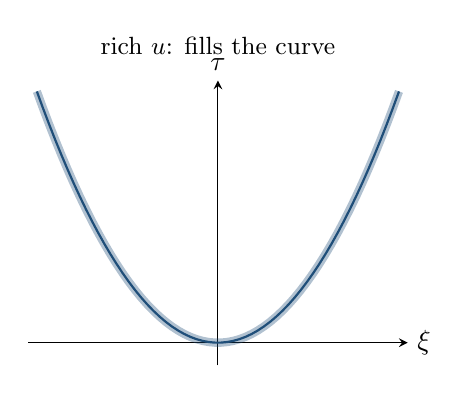
\begin{tikzpicture}
\begin{axis}[width=6.4cm,height=5.2cm,axis lines=middle,xlabel={$\xi$},ylabel={$\tau$},xmin=-2.2,xmax=2.2,ymin=-0.4,ymax=4.6,
 ticks=none,title={\small rich $u$: fills the curve},every axis x label/.style={at={(current axis.right of origin)},anchor=west},
 every axis y label/.style={at={(current axis.above origin)},anchor=south}]
\addplot[cA,line width=3pt,opacity=0.35,domain=-2.1:2.1,samples=60] {x^2};
\addplot[cA,thick,domain=-2.1:2.1,samples=60] {x^2};
\end{axis}
\end{tikzpicture}\hfill
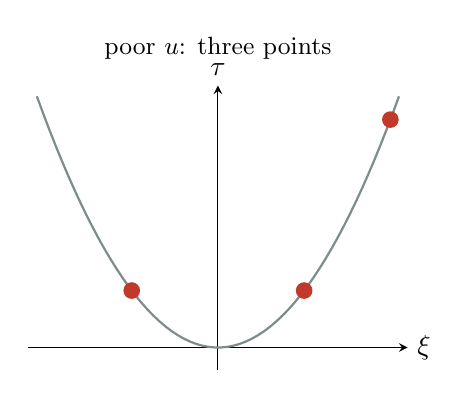
\begin{tikzpicture}
\begin{axis}[width=6.4cm,height=5.2cm,axis lines=middle,xlabel={$\xi$},ylabel={$\tau$},xmin=-2.2,xmax=2.2,ymin=-0.4,ymax=4.6,
 ticks=none,title={\small poor $u$: three points},every axis x label/.style={at={(current axis.right of origin)},anchor=west},
 every axis y label/.style={at={(current axis.above origin)},anchor=south}]
\addplot[cG,thick,domain=-2.1:2.1,samples=60] {x^2};
\addplot[only marks,mark=*,cB,mark size=2.8pt] coordinates {(1,1) (-1,1) (2,4)};
\end{axis}
\end{tikzpicture}
\caption{The heat curve $\tau=\xi^2$. Left: a solution that is not an exponential-polynomial (the heat kernel) uses the whole curve, and $\Ann(u)=(P)$. Right: a finite sum of exponentials lives on finitely many points. Then $\Ann(u)$ contains polynomials that vanish at those points but are not multiples of $P$.}\label{fig:rich-poor}
\end{figure}

\begin{proposition}[{Uniqueness of the identified operator}]\label{f:prop:unique}
If $\Ann(u)=(P)$, then every operator $Q$ with $Q(\partial)u=0$ is a multiple $Q=SP$ with $S\in\ring$. In particular $P$ is, up to a nonzero constant, the only annihilator of minimal degree.

\dimref{C3-T1}
\end{proposition}

The proof is one line: $Q\in(P)$ means $Q=SP$, and degrees add, so $\deg Q\ge\deg P$ with equality only when $S$ is a constant.

\begin{example}[{The heat equation, three cases}]\label{ex:heat3}
Take $P=\tau-D\xi^2$ with $D>0$. It is irreducible, so $P/P_1=1$ and the criterion reads
\[
\Ann(u)=(P)\iff u\notin\EP .
\]

\textbf{One Fourier mode.} Let $u=e^{-D\kappa^2t+i\kappa x}$. Then $u_t=-D\kappa^2u$ and $u_{xx}=-\kappa^2u$. So $u$ is also killed by $\partial_x-i\kappa$ and by $\partial_t+D\kappa^2$:
\[
\Ann(u)=(\tau+D\kappa^2,\ \xi-i\kappa).
\]
This is the ideal of one point of $\Var(P)$, strictly larger than $(P)$. Indeed $P$ belongs to it:
\[
P=(\tau+D\kappa^2)-D\,(\xi-i\kappa)(\xi+i\kappa).
\]

\textbf{A finite superposition.} For $u=\sum_{j=1}^rc_je^{-D\kappa_j^2t+i\kappa_jx}$ with distinct $\kappa_j$, $u\in\EP$. Its annihilator is the ideal of the $r$ points $(-D\kappa_j^2,\,i\kappa_j)$. It contains many operators that are not multiples of $P$.

\textbf{The heat kernel.} Let $u=t^{-1/2}e^{-x^2/(4Dt)}$ for $t>0$. Its $x$-derivatives are polynomials of growing degree times the same Gaussian. They span an infinite-dimensional space, so $u\notin\EP$ (Lemma~\ref{f:lem:ep}). Hence $\Ann(u)=(P)$: every constant-coefficient equation satisfied by the heat kernel is a multiple of $\tau-D\xi^2$.

\emph{Message.} A ``poor'' solution remembers only finitely many exponentials and cannot tell the heat equation from many others. A ``rich'' solution remembers the whole equation.
\end{example}

\begin{example}[{The wave equation and d'Alembert \led{C3-T5} \proved}]\label{ex:wave-ident}
Let $P=(\tau-c\xi)(\tau+c\xi)$ with real $c\ne0$, and $u=f(x-ct)+g(x+ct)$. The two partial quotients are
\begin{align*}
w_1&=(\partial_t+c\partial_x)\,u=2c\,g'(x+ct),\\
w_2&=(\partial_t-c\partial_x)\,u=-2c\,f'(x-ct).
\end{align*}
So the criterion says:
\[
\Ann(u)=(P)\iff f\notin\EP\ \text{ and }\ g\notin\EP .
\]
A single travelling wave ($g=0$) never identifies the wave equation: it also satisfies the first-order transport equation. The same theorem covers Klein--Gordon $\tau^2-\xi^2+\mu^2$ and the telegraph operator $\tau^2+\alpha\tau-c^2\xi^2$: both are irreducible conics, so they are identified iff $u\notin\EP$. For the beam $\tau^2+\xi^4=(\tau-i\xi^2)(\tau+i\xi^2)$ both Schr\"odinger parts must be outside $\EP$.

\dimref{C3-T5}
\end{example}

\begin{takeaway}
Theorem~\ref{f:thm:ident} turns ``does $u$ identify $P$?'' into finitely many membership tests ``$\in\EP$''. Each test is a finite-dimensional computation (Lemma~\ref{f:lem:ep}). Whether the tests can be carried out from the data one actually has is the subject of Section~\ref{f:ch:data}.
\end{takeaway}

\subsection{The intrinsic operator and the spectral form}\label{sec:spectral}

Theorem~\ref{f:thm:ident} says when $(P)$ is the whole annihilator. When it is not, what does $u$ determine? The answer uses the two pieces of $\Ann(u)$ given by Lemma~\ref{f:lem:gcd}.

\begin{notebox}{Point spectrum}
Recall $\Ann(u)=G_u\,J_u$ with $G_u=\Gcd\Ann(u)$. The \emph{point spectrum} of $u$ is the finite set
\[
\sigma_p(u)=\Var(J_u)\subset\C^2 .
\]
Its points are the exponents $(\tau_0,\xi_0)$ of the exponentials $e^{\tau_0t+\xi_0x}$ that are ``present'' in $u$. The word spectrum is meant in the algebraic sense, not as the spectrum of an operator on a Hilbert space. We write $G_u\sim P$ when the two agree up to a nonzero constant.
\end{notebox}

\begin{theorem}[{Spectral characterisation \led{P4-T2} \proved}]\label{thm:spec}
Let $P$ be an annihilator of $u$. Then
\[
\Ann(u)=(P)\iff \sigma_p(u)=\emptyset\ \text{ and }\ G_u\sim P .
\]
Moreover the exponential-polynomial part of the derivative space is the finite quotient
\[
\ring u\cap\EP\;\cong\;\ring/J_u .
\]
\dimref{P4-T2}
\end{theorem}

\begin{example}[{Reading the spectrum}]
\textbf{One exponential.} For $u=e^{\tau_0t+\xi_0x}$: $\Ann(u)=(\tau-\tau_0,\ \xi-\xi_0)$, so $G_u=1$ and $\sigma_p(u)=\{(\tau_0,\xi_0)\}$. A single exponential has no infinite part and a one-point spectrum.

\textbf{Two exponentials.} For $u=e^{\tau_1t+\xi_1x}+e^{\tau_2t+\xi_2x}$ with distinct exponents: $G_u=1$ and $\sigma_p(u)$ has two points.

\textbf{A rich solution.} If $\Ann(u)=(P)$ then $\sigma_p(u)=\emptyset$ and $G_u\sim P$.
\end{example}

The operator $G_u$ is the correct ``operator intrinsic to $u$''. It depends only on $u$, while $P$ depends on which annihilator was chosen. The next theorem computes it from any annihilator.

\begin{theorem}[{Intrinsic operator \led{C3-T6} \proved}]\label{thm:intrinsic}
Let $P=c\prod_iP_i^{e_i}$ be any annihilator of $u$. For each $i$ let
\[
k_i=\max\Big\{k\le e_i:\ \Big(\frac{P}{P_i^{k}}\Big)(\partial)u\in\EP\Big\}
\]
(with $k_i=0$ if no such $k\ge1$ exists), and $f_i=e_i-k_i$. Then
\[
G_u\sim\prod_iP_i^{f_i},
\]
and $\Ann(u)$ is principal if and only if $G_u(\partial)u=0$. Computing $G_u$ takes at most $\sum_ie_i$ tests ``$\in\EP$''.

\dimref{C3-T6}
\end{theorem}

\begin{example}[{A repeated factor}]
Let $G$ be the heat kernel ($D=1$), $P=(\tau-\xi^2)^3$ and $u=t\,G$. Then:
\begin{align*}
\Big(\frac{P}{P_1}\Big)(\partial)u&=(\partial_t-\partial_x^2)^2(tG)=0\in\EP,\\
\Big(\frac{P}{P_1^2}\Big)(\partial)u&=(\partial_t-\partial_x^2)(tG)=G\notin\EP .
\end{align*}
So $k_1=1$, $f_1=2$, and
\[
G_u=(\tau-\xi^2)^2,\qquad \Ann(u)=(G_u).
\]
The function $tG$ identifies the \emph{square} of the heat operator, not its cube.
\end{example}

\begin{caution}[title={Why $G_u$ and not the variety}]
A tempting stronger statement replaces $G_u$ by the variety $\Var(\Ann u)$. It is correct only for reduced $P$, because zero sets do not see multiplicities.

\emph{Example.} Let $P=\tau^2$ and $u=e^{x^2}$. Then $u_{tt}=0$. No nonzero polynomial in $\partial_x$ alone kills $u$, so
\[
\Ann(u)=(\tau).
\]
Here $\sigma_p(u)=\emptyset$, but $G_u=\tau\not\sim P$. So $\Ann(u)\ne(P)$, while $\Var(\Ann u)=\{\tau=0\}=\Var(P)$. The variety alone would wrongly say that $u$ identifies $\tau^2$.
\end{caution}

\subsection{Refinements}

\subsubsection{Evolutions: identification inside a finite class}

For an evolution $u_t=a(\partial_x)u$ the symbol $P=\tau-a(\xi)$ has degree one in $\tau$, so it is irreducible. The criterion says: $\Ann(u)=(P)$ iff $u\notin\EP$. When $u$ \emph{is} an exponential-polynomial, we can still ask whether $a$ is recovered among polynomials of degree at most $n$.

\begin{theorem}[{Evolutions \led{C3-T4} \proved}]\label{thm:evol}
Let $P=\tau-a(\xi)$ and $P(\partial)u=0$ on a connected $\Omega$.
\begin{enumerate}[label=(\alph*)]
\item $\Ann(u)=(P)$ if and only if $u\notin\EP(\Omega)$.
\item If $u=\sum_kq_k\,e^{\tau_kt+\xi_kx}$ with distinct exponents and nonzero $q_k$, put $\delta_k=\deg_xq_k$ and
\[
D=\sum_k(\delta_k+1).
\]
If $\deg a\le n$, then among all $b$ of degree at most $n$, the evolutions $\tau-b$ that kill $u$ are exactly
\[
b\in a+\prod_k(\xi-\xi_k)^{\delta_k+1}\cdot\C[\xi]_{\le n-D}.
\]
So $a$ is identified in degree $\le n$ if and only if $D\ge n+1$.
\end{enumerate}
\dimref{C3-T4}
\end{theorem}

This is Hermite interpolation: a polynomial of degree $n$ is fixed by $n+1$ conditions, and each mode $q_k\,e^{\tau_kt+\xi_kx}$ supplies $\delta_k+1$ of them.

\begin{example}[{Advection--diffusion from two modes}]
Take $u_t=-cu_x+Du_{xx}$, so $a(\xi)=-c\xi+D\xi^2$ has degree $n=2$. Two simple modes give $D=2<3$: the pair $(c,D)$ is not identified, because one free parameter remains. Three distinct modes give $D=3$: both coefficients are fixed.
\end{example}

\subsubsection{A naive transfer that fails}

On a periodic domain an earlier result said: if the Fourier expansion of $u$ has infinitely many frequencies on every factor curve, then $\Ann(u)=(P)$ \led{R4-T5}. On a \emph{bounded} domain this transfer is false, because the expansion is not unique.

\begin{falsebox}{The spectrum of an expansion is not intrinsic \led{C3-C1} \falsest}\label{cex:C3C1}
Let $P=\tau+\xi$ and $\Omega=(0,1)^2$. On $(-\pi,\pi)$ the Fourier series
\[
e^{s}=\sum_{k\in\Z}c_k\,e^{iks},\qquad c_k=\frac{\sinh(\pi)(-1)^k}{\pi(1-ik)}\neq0,
\]
converges in $L^2$. So $u=e^{x-t}=\sum_kc_k\,e^{ik(x-t)}$ has infinitely many exponents on the line $\tau+\xi=0$. Yet
\[
\Ann(u)=(\tau+1,\ \xi-1)\supsetneq(\tau+\xi).
\]
\dimref{C3-C1}
\end{falsebox}

The criterion must therefore be stated on $u$ itself, as in Theorem~\ref{f:thm:ident}, not on an expansion of $u$.

\subsubsection{Symmetries and local data}

\begin{proposition}[{Translation symmetry \led{C3-P3} \pw}]\label{prop:sym}
Suppose $u$ is invariant under translations along a direction, $\ell(\partial)u=0$ with $\ell=\alpha\tau+\beta\xi\ne0$, and $P(\partial)u=0$ with $P$ nonconstant. If $P\not\sim\ell$, then $\Ann(u)\ne(P)$. If moreover $\ell\nmid P$, then $u\in\EP$.

\dimref{C3-P3}
\end{proposition}

So a symmetry with constant characteristic destroys identification, and it is a special case of the criterion. Symmetries with variable coefficients are invisible in $\C[\partial]$: the heat kernel is scale invariant, $(2t\partial_t+x\partial_x+1)G=0$, yet $\Ann(G)=(\tau-\xi^2)$. Identifiability depends on the ring of coefficients.

\begin{proposition}[{Local data \led{C3-P5} \pw}]\label{prop:local}
Identification can be lost on a smaller region. Let $P=\tau+\xi$, $F(s)=e^s+\varphi(s)$ with $\varphi$ a smooth bump supported in $(2,3)$, and $u=F(x-t)$. On $(0,1)\times(-5,5)$, $u\notin\EP$ and $\Ann(u)=(\tau+\xi)$. On the smaller square $(0,1)^2$, $u=e^{x-t}$ and the annihilator is the ideal of a point.

For elliptic $P$, every solution is real-analytic, and then $\Ann(u|_{\Omega'})=\Ann(u)$ for every connected $\Omega'\subset\Omega$.

\dimref{C3-P5}
\end{proposition}

\begin{keypoint}
A solution identifies its equation exactly when, after removing any one irreducible factor, what is left is not a finite sum of exponentials. In general, $u$ identifies only its intrinsic operator $G_u$. The difference between $P$ and $G_u$ is a finite set of exponentials, the point spectrum $\sigma_p(u)$.
\end{keypoint}


% ---- end sections/full_ch4.tex


% ---- begin sections/full_ch5.tex
\section{Finite data and decidability}\label{f:ch:data}
\sectionbrief
{the criterion of Section~\ref{f:ch:ident}: $\Ann(u)=(P)$ iff no $w_i$ is an exponential-polynomial. It is a statement about the whole function $u$.}
{in practice we hold finitely many numbers: a jet at a point, samples, or a formula. We ask which data suffice, which never suffice, and when the test ``$\in\EP$'' becomes an algorithm.}
{tells Step~3 of the algorithm what it can and cannot promise. The answer depends on the data model: positive for exponential-polynomials, negative for a black box, positive again with one extra integer.}

\subsection{Three data models}

The reconstruction is exact, so the input must be of an exact kind. Three models are analysed throughout \led{C3-D1}.

\begin{description}[leftmargin=1.4cm,labelwidth=1.1cm,font=\sffamily\bfseries]
\item[M1] A closed formula for $u$, for example a finite sum of exponentials and Gaussians.
\item[M2] The jet of $u$ at a point $p_0$: all partial derivatives up to some order, given as exact numbers. In the ``black-box'' version M2$^+$ we may also ask a \emph{zero-test oracle} whether $Q(\partial)u=0$ for a given $Q$.
\item[M3] $u$ real-analytic on a connected $\Omega$, described by finitely many linear equations with polynomial coefficients (a \emph{holonomic} description) with algebraic numbers as coefficients.
\end{description}

\begin{notebox}{Words used in this chapter}
\begin{description}[leftmargin=3.3cm,labelwidth=3.1cm]
\item[Jet of order $k$] the list of all partial derivatives of $u$ of order $\le k$ at $p_0$: its Taylor coefficients.
\item[Zero-test oracle] a procedure that says whether a given expression built from $u$ is identically zero.
\item[Holonomic] described by linear differential equations with polynomial coefficients whose solution space is finite-dimensional.
\item[Weyl algebra] $A_1$ or $A_2$: the ring of differential operators with polynomial coefficients.
\end{description}
\end{notebox}

\subsection{Exponential-polynomial data: a finite threshold}

When $u$ itself is an exponential-polynomial, it never identifies its equation in the whole ring: its annihilator has finitely many zeros, while $\Var(P)$ is a curve \led{C3-C2}. What we can ask is whether $u$ identifies $P$ \emph{among operators of degree at most $n$}.

\begin{theorem}[{B\'ezout threshold \led{C3-T2} \proved}]\label{thm:bezout}
Let $u=\sum_kc_k\,e^{\langle z_k,(t,x)\rangle}$ be a sum of simple modes with distinct exponents $z_k\in\Var(P)$, $P$ reduced, and $n\ge\deg P$. If every factor curve carries enough exponents,
\[
\big|\{z_k\}\cap\Var(P_i)\big|>n\cdot\deg P_i\qquad\text{for every }i,
\]
then the annihilators of degree at most $n$ are exactly the multiples of $P$:
\[
\Ann(u)\cap\ring_{\le n}=P\cdot\ring_{\le n-\deg P}.
\]
The threshold cannot be lowered uniformly: for $P=\tau-\xi^2$ and every $n$ there are $2n$ exponents on the parabola that do not suffice.

\dimref{C3-T2}
\end{theorem}

\begin{intuition}
An operator $Q$ of degree $n$ that kills $u$ must vanish at every exponent $z_k$. If $P_i$ does not divide $Q$, the two curves meet in at most $n\deg P_i$ points (B\'ezout). More points than that force $P_i$ to divide $Q$.
\end{intuition}

\begin{example}[{The parabola needs $2n+1$ points}]
Let $P=\tau-\xi^2$, so $\deg P=2$. Take the $2n$ exponents
\[
Z_n=\{(j^2,\pm j):\ j=1,\dots,n\}\subset\Var(P).
\]
The operator $Q_n=\prod_{j=1}^n(\tau-j^2)$ has degree $n$, vanishes on $Z_n$, and is not a multiple of $\tau-\xi^2$ because it does not depend on $\xi$. So $2n$ points are not enough. With $2n+1$ points the theorem applies.
\end{example}

The next theorem says how many derivatives at a single point are needed.

\begin{theorem}[{Jet threshold $2d-1$ \led{C3-T3} \proved}]\label{thm:jet-threshold}
Let $0\ne u\in\EP(\Omega)$ on a connected $\Omega$, and let $d=\dimc\ring u$. Then:
\begin{enumerate}[label=(\roman*)]
\item the operators of degree at most $n$ that kill $u$ are determined by the jet of $u$ of order $n+d-1$ at any point;
\item $\Ann(u)$ is generated in degree at most $d$, so it is determined by the jet of order $2d-1$;
\item the order $2d-1$ is optimal in the worst case, already in one variable: for $u=\sum_{j=1}^de^{jx}$ the jet of order $2d-2$ does not determine $\Ann(u)$.
\end{enumerate}
An upper bound $d'\ge d$ may replace $d$ everywhere.

\dimref{C3-T3}
\end{theorem}

\begin{example}[{One exponential, $d=1$}]
For $u=e^{2x}$, $d=1$ and the threshold is $2d-1=1$. The values $u(0)=1$ and $u'(0)=2$ give $u'=2u$, so $\Ann(u)$ contains $\xi-2$, and $\tau$ comes from the absence of $t$. The value $u(0)$ alone (order $0$) cannot distinguish $e^{2x}$ from $e^{3x}$.
\end{example}

\subsection{What no finite data can show}

For a solution outside $\EP$, the situation reverses.

\begin{theorem}[{No finite certificate \led{C3-P1} \proved{} / \cf}]\label{f:thm:nocert}
Let $\Omega$ be connected, $P$ nonconstant and $u\in\ker P$. For every order $K$ there is an exponential-polynomial $v\in\ker P$ with the same jet of order $K$ at $p_0$ as $u$, and $\Ann(v)\ne(P)$.

On convex $\Omega$ the same holds for any finite family of continuous linear functionals (Malgrange's density theorem) \cf. On a non-convex region a single functional can certify.

\dimref{C3-P1}
\end{theorem}

\begin{intuition}
Every finite jet is matched by a finite sum of exponentials taken from the curve $\Var(P)$. Finitely many numbers cannot distinguish $u$ from that sum, and the sum never identifies anything. So an algorithm that sees finitely many numbers can only \emph{refute} identification, never confirm it.
\end{intuition}

The black-box version is sharper.

\begin{theorem}[{Black-box impossibility \led{P4-T5} \proved}]\label{f:thm:blackbox}
In the model M2$^+$ (exact jets plus a zero-test oracle), for every nonconstant $P$ there is a solution $u$ with $\Ann(u)=(P)$ such that the following holds. For every jet order $k_0$ and every finite set of zero tests, some exponential-polynomial $v\in\ker P$ gives the same jet and the same answers, while $\Ann(v)\ne(P)$. Hence no algorithm decides ``$\Ann(u)=(P)$'' correctly on all inputs.

\dimref{P4-T5}
\end{theorem}

\subsection{One extra integer makes it decidable}

\begin{theorem}[{Decidability with a bound \led{P4-T4} \proved}]\label{thm:decide}
In the model M2$^+$:
\begin{enumerate}[label=(\roman*)]
\item for every finite-dimensional space of operators $\mathcal L$, the annihilators of $u$ in $\mathcal L$ are computable;
\item ``$\Ann(u)\ne(P)$'' is semi-decidable: an algorithm stops with ``yes'' exactly when it is true;
\item if an integer $B\ge\dimc(\ring u\cap\EP)$ is given, ``$\Ann(u)=(P)$'' is decidable. With
\[
N=B+\deg P-1,
\]
one has $\Ann(u)=(P)$ iff $\Ann(u)\cap\ring_{\le N}=(P)\cap\ring_{\le N}$.
\end{enumerate}
The bound also makes $G_u$ computable.

\dimref{P4-T4}
\end{theorem}

\begin{intuition}
If identification fails, some $w_i$ is an exponential-polynomial of dimension at most $B$. Its annihilator has a generator of degree at most $B$ that is not a multiple of $P_i$. Multiplying by $P/P_i$ gives a witness of degree at most $B+\deg P-1$. So it is enough to look for witnesses up to that degree, and that is a finite linear-algebra problem.
\end{intuition}

Is the bound $B$ the least data that works? The minimal sufficient datum is ``a degree $D$ such that, if identification fails, a witness of degree $\le D$ exists'' \led{OP-ALG-T3} \pw. The bound $B$ is strictly stronger on some regions when $P$ has at least two irreducible factors counted with multiplicity. Whether it is strictly stronger on every region is open \openq{} \led{OP-ALG-Q2}.

\subsection{A decidable class: holonomic solutions}

\begin{theorem}[{Holonomic model \led{OP-ALG-T1, P4-T6} \modulo{(AC)}}]\label{thm:holo}
In the model M3 (real-analytic $u$ with a holonomic description over algebraic numbers), assume (AC): jets at an algebraic point are computable in a computable field. Then
\begin{itemize}
\item ``$Q(\partial)u\in\EP$?'' is decidable for every $Q$;
\item ``$\Ann(u)=(P)$?'' and ``$\Var(\Ann u)=\Var(P)$?'' are decidable, and $G_u$ is computable;
\item a bound $B$ and a finite set of generators of $\Ann(u)$ are computable.
\end{itemize}
\dimref{OP-ALG-T1}
\end{theorem}

\begin{example}[{The heat kernel plus an exponential}]
Let $u=G+e^{t+x}$, with $G$ the heat kernel. The slice $t=1$ is $x\mapsto G(1,x)+e^{1+x}$, a function with a holonomic description. The algorithm finds that the slice is not an exponential-polynomial, and concludes $\Ann(u)=(\tau-\xi^2)$. For the slice of $G$ alone the bound is $B=0$: the heat kernel identifies the heat equation without further computation.
\end{example}

\subsection{Variable coefficients: the first limits}

With coefficients that depend on $x$, the ring of operators becomes the Weyl algebra. Two of its features break the constant-coefficient picture.

\begin{proposition}[{Restriction does not identify \led{P4-C1} \pw}]\label{prop:weyl}
For every nonzero smooth $u$ of one variable, the action of the Weyl algebra $A_1$ on the module $A_1\cdot u$ is faithful. Yet for $u=e^x$ and the class $\mathcal L=\spn\{1,\partial\}$, the operator $\partial-1$ kills $u$. So ``the restriction is injective'' does not detect identification. The correct object is the evaluation map $L\mapsto Lu$, whose kernel is $\Ann(u)\cap\mathcal L$.

\dimref{P4-C1}
\end{proposition}

\begin{theorem}[{Saturated criterion \led{OP-ALG-T4} \pw}]\label{thm:sat}
Let $P$ be monic in $\partial_t$ of degree $m$, with coefficients in a ring $\mathfrak A$ of operators in $x$, and $Pu=0$. Then $u$ identifies $P$ if and only if the $t$-jet $u,\partial_tu,\dots,\partial_t^{m-1}u$ is free over $\mathfrak A$: no nontrivial relation $\sum_{j<m}b_j\,\partial_t^ju=0$ with $b_j\in\mathfrak A$.

\dimref{OP-ALG-T4}
\end{theorem}

In the commutative case this is Proposition~\ref{prop:cyclic}. With variable coefficients the reduction of the test to the finitely many quotients $P/P_i$ fails: an explicit counterexample with $\theta=x\partial_x$ exists \led{OP-ALG-C1} \pw. In the full Weyl algebra $A_2$, a holonomic solution never identifies its equation \led{OP-ALG-P5} \pw.

\subsection{Summary}

\begin{center}\small
\begin{tabular}{@{}L{3.0cm}L{5.2cm}L{4.4cm}L{2.0cm}@{}}
\toprule
Data & What can be done & Meaning for the algorithm & Status\\\midrule
$u\in\EP$ & jet of order $2d-1$ determines $\Ann(u)$; Bézout threshold for modes & a finite computation with a guarantee & \proved\\
$u\notin\EP$, finite data & no finite certificate & output ``not refuted'', never ``identified'' & \proved{} / \cf\\
black box & ``$\in\EP$?'' undecidable & extra hypothesis needed & \proved\\
bound $B$ given & decidable, test degree $B+\deg P-1$ & stops with a certain verdict & \proved\\
holonomic, algebraic & decidable & exact symbolic route & \modulo{(AC)}\\
variable coefficients & restriction never identifies; jet freeness criterion & restrict to a finite class & \pw\\\bottomrule
\end{tabular}
\captionof{table}{When the identification test can be carried out, and what each case means for Step~3 of the algorithm.}\label{tab:limits}
\end{center}

\begin{keypoint}
Identification is an infinite statement about $u$. It cannot be verified from finitely many numbers, and no black box can decide it. One extra integer, a bound on how much of $u$ is exponential-polynomial, turns it into a finite computation.
\end{keypoint}


% ---- end sections/full_ch5.tex


% ---- begin sections/full_ch6.tex
\section{Decomposition into components}\label{f:ch:decomp}
\sectionbrief
{the operator is known and factored: $P=c\prod_{j=1}^sQ_j$ with $Q_j=P_j^{m_j}$ pairwise coprime. For the main theorem $\Omega$ is open, connected and simply connected (more precisely $H^1_{dR}(\Omega)=0$).}
{once $P$ is known, we want to split $u$ into the parts generated by each piece of $P$, so that the pieces can be studied separately.}
{second link of the chain. The split exists for \emph{factors} of the symbol, with a finite and exactly known ambiguity. It fails for additive \emph{terms}, and that failure is what Section~\ref{f:ch:interaction} measures.}

\subsection{Which pieces? Terms versus factors}

An operator can be broken up in two different ways. Take the heat operator
\[
L=\partial_t-D\partial_x^2 .
\]
Its \emph{terms} are $L_1=\partial_t$ and $L_2=-D\partial_x^2$: they are added. Its symbol $\tau-D\xi^2$ is irreducible, so it has only one \emph{factor}. For the wave operator the situation is the opposite: $\tau^2-\xi^2$ has two terms and also two factors, $\tau-\xi$ and $\tau+\xi$. The first question is which kind of piece gives a decomposition of the solution.

\subsubsection{Terms do not give components}

\begin{proposition}[{Splitting by terms fails \led{R2-T3} \proved}]\label{f:prop:terms}
Let $L=L_1+L_2$ with constant coefficients. If $u=a+b$ with $L_1a=0$ and $L_2b=0$ solves $Lu=0$, then $u$ is also killed by $L_1L_2$:
\[
\ker L\cap(\ker L_1+\ker L_2)\ \subseteq\ \ker(L,\ L_1L_2).
\]
The common zero set of $L$ and $L_1L_2$ is $\Var(L_1)\cap\Var(L_2)$. When this set is finite, only a finite-dimensional space of exponential-polynomial solutions can be split by terms.

\dimref{R2-T3}
\end{proposition}

\begin{intuition}
The two operators commute, so
\[
L_1L_2\,u=L_2(L_1a)+L_1(L_2b)=0 .
\]
A solution split by terms satisfies one extra equation. A generic solution does not.
\end{intuition}

\begin{example}[{The heat equation cannot be split by terms}]
Take $L_1=\partial_t$ and $L_2=-D\partial_x^2$. The kernels are
\[
\ker L_1=\{f(x)\},\qquad \ker L_2=\{a(t)+b(t)\,x\}.
\]
Every element $f(x)+a(t)+b(t)x$ of the sum is killed by $\partial_t\partial_x^2$. A heat solution is not. For $u=e^{-D\kappa^2t}\cos\kappa x$:
\[
\partial_x^2u=-\kappa^2u,\qquad \partial_t\partial_x^2u=D\kappa^4u\neq0 .
\]
So a generic heat solution is \emph{not} a sum of a solution of $u_t=0$ and a solution of $u_{xx}=0$.

The exceptions are few. The function $u=\tfrac12x^2+Dt$ solves the heat equation and lies in $\ker L_1+\ker L_2$, but it is a polynomial: the exceptional space is finite-dimensional.
\end{example}

\subsubsection{Factors do give components}

\begin{example}[{The wave equation and d'Alembert}]\label{ex:wave}
Let $c>0$ and
\[
P=\tau^2-c^2\xi^2=(\tau-c\xi)(\tau+c\xi)=Q_1Q_2 .
\]
A direct check gives
\[
(\partial_t-c\partial_x)\,f(x+ct)=0,\qquad (\partial_t+c\partial_x)\,g(x-ct)=0 .
\]
So $\ker Q_1=\{f(x+ct)\}$ (profiles moving left) and $\ker Q_2=\{g(x-ct)\}$ (profiles moving right). D'Alembert's formula says that every solution is a sum of the two:
\[
\ker P=\ker Q_1+\ker Q_2 .
\]
The pieces are unique up to a constant: $f\mapsto f+k$, $g\mapsto g-k$. This ambiguity has dimension $1$, and it equals $\dimc\ring/(Q_1,Q_2)$:
\[
Q_1+Q_2=2\tau,\qquad Q_2-Q_1=2c\xi\quad\Longrightarrow\quad(Q_1,Q_2)=(\tau,\xi),\qquad \ring/(\tau,\xi)\cong\C .
\]
\end{example}

\begin{figure}[!htb]
\centering
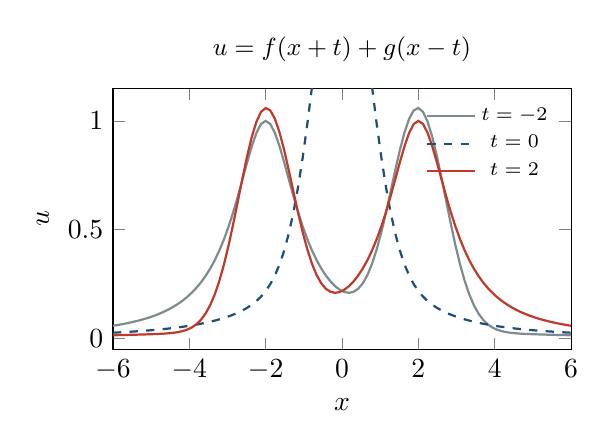
\begin{tikzpicture}
\begin{axis}[width=7.4cm,height=4.9cm,xlabel={$x$},ylabel={$u$},xmin=-6,xmax=6,ymin=-0.05,ymax=1.15,legend style={font=\scriptsize,at={(0.98,0.97)},anchor=north east,draw=none,fill=none},
 title={\small $u=f(x+t)+g(x-t)$},domain=-6:6,samples=100,no markers]
\addplot[cG,thick] {1/(1+(x+2)^2)+exp(-(x-2)^2)};
\addplot[cA,thick,dashed] {1/(1+(x+0)^2)+exp(-(x-0)^2)};
\addplot[cB,thick] {1/(1+(x-2)^2)+exp(-(x+2)^2)};
\legend{$t=-2$,$t=0$,$t=2$}
\end{axis}
\end{tikzpicture}
\hfill
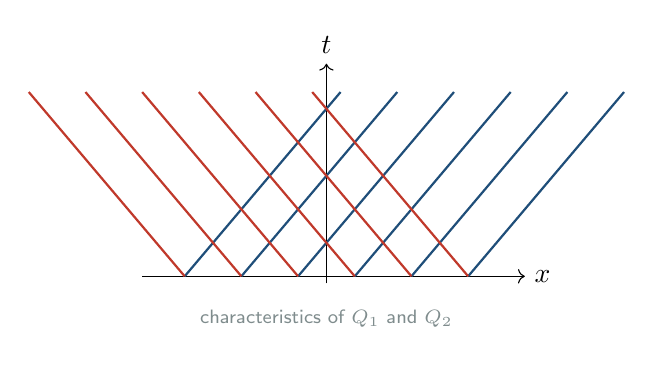
\begin{tikzpicture}[scale=0.9]
\draw[->] (-2.6,0)--(2.8,0) node[right]{$x$}; \draw[->] (0,-0.1)--(0,3) node[above]{$t$};
\foreach \a in {-2,-1.2,-0.4,0.4,1.2,2}{
  \draw[cA,thick] (\a,0)--(\a+2.2,2.6); \draw[cB,thick] (\a,0)--(\a-2.2,2.6);}
\node[font=\scriptsize\sffamily,text=cG] at (0,-0.6) {characteristics of $Q_1$ and $Q_2$};
\end{tikzpicture}
\caption{Left: the d'Alembert solution with $f(s)=1/(1+s^2)$ moving left and $g(s)=e^{-s^2}$ moving right ($c=1$). Right: the two families of characteristic lines, one per factor. Each factor of the symbol carries one rigidly translating component.}\label{fig:wave}
\end{figure}

\subsection{Why factors work: the Chinese remainder theorem}

\textbf{One variable.} If two polynomials $Q_1,Q_2$ in one variable are coprime, there are polynomials $a,b$ with
\[
a\,Q_1+b\,Q_2=1 .
\]
Then every $u$ with $Q_1Q_2u=0$ splits explicitly as
\[
u=\underbrace{b\,Q_2\,u}_{\in\ker Q_1}+\underbrace{a\,Q_1\,u}_{\in\ker Q_2},
\]
and the sum of the two kernels is direct.

\textbf{Two variables.} ``Coprime'' now means only that the common zeros are finitely many (B\'ezout), not that $(Q_1,Q_2)=\ring$. The finite quotient $\ring/(Q_1,Q_2)$ measures the failure of the one-variable picture.

\begin{lemma}[{Finite quotient \led{C12-L3} \proved}]\label{lem:C12L3}
Let $f,g,h\in\ring\setminus\{0\}$.
\begin{enumerate}[label=(\alph*)]
\item If $f,g$ are coprime, the ideal $(f,g)$ contains a nonzero polynomial in $\xi$ alone and a nonzero polynomial in $\tau$ alone. Hence $\dimc\ring/(f,g)<\infty$.
\item If $f$ is coprime to $g$ and to $h$, then
\[
\dimc\ring/(f,gh)=\dimc\ring/(f,g)+\dimc\ring/(f,h).
\]
\item $(f,g)=\ring$ if and only if $\Var(f)\cap\Var(g)=\emptyset$.
\end{enumerate}
\dimref{C12-L3}
\end{lemma}

The geometric meaning of $\dimc\ring/(Q_i,Q_j)$ is the number of crossing points of the curves $\Var(Q_i)$ and $\Var(Q_j)$, counted with intersection multiplicity.

\subsection{The decomposition theorem}

\begin{theorem}[{Factor decomposition \led{C12-T1, C12-T1$'$} \proved}]\label{f:thm:factor}
Let $\Omega\subset\R^2$ be open, connected, with $H^1_{dR}(\Omega)=0$ (for example simply connected: a rectangle, a convex set, a slit disc). Let $\mathcal A$ be $\mathcal D'(\Omega)$ or $C^\infty(\Omega)$, and $P=c\prod_{j=1}^sQ_j$ with pairwise coprime $Q_j$. Then:
\begin{enumerate}[label=(\roman*)]
\item every solution splits:
\[
\ker_{\mathcal A}P=\ker_{\mathcal A}Q_1+\dots+\ker_{\mathcal A}Q_s ;
\]
\item the ambiguity (the $s$-tuples of components with sum $0$) has dimension exactly
\[
\delta(P)=\sum_{i<j}\dimc\ring/(Q_i,Q_j),
\]
and consists of exponential-polynomials;
\item the splitting is unique if and only if $\Var(Q_i)\cap\Var(Q_j)=\emptyset$ for all $i\ne j$.
\end{enumerate}
\dimref{C12-T1p}
\end{theorem}

\begin{intuition}
At a crossing point $z$ of two factor curves, the exponential $e^{\langle z,(t,x)\rangle}$ belongs to both kernels. It can be moved freely from one component to the other. The number of such free moves, counted with multiplicity, is $\delta(P)$.

Algebraically the proof uses the exact sequence
\[
0\to\ring/(Q_1Q_2)\to\ring/(Q_1)\oplus\ring/(Q_2)\to\ring/(Q_1,Q_2)\to0
\]
and shows that applying $\mathrm{Hom}(\,\cdot\,,\mathcal A)$ keeps it exact. The only possible obstruction lives on the finite-dimensional module $\ring/(Q_1,Q_2)$, and it vanishes when $\Omega$ has no holes (Lemma~\ref{lem:twisted}).
\end{intuition}

\begin{example}[{The ambiguity on four operators}]
\begin{center}\small
\begin{tabular}{@{}L{3.0cm}L{4.4cm}L{1.0cm}L{4.4cm}@{}}
\toprule
Operator & Factors & $\delta(P)$ & Ambiguity\\\midrule
wave $\tau^2-\xi^2$ & $\tau-\xi,\ \tau+\xi$ & $1$ & constants\\
beam $\tau^2+\xi^4$ & $\tau-i\xi^2,\ \tau+i\xi^2$ & $2$ & $\spn\{1,x\}$\\
heat--transport & $\tau-\xi^2,\ \tau-\xi$ & $2$ & $\spn\{1,\ e^{t+x}\}$\\
parallel transports & $\tau-\xi,\ \tau-\xi-1$ & $0$ & none (unique)\\\bottomrule
\end{tabular}
\end{center}
For heat--transport the curves $\tau=\xi^2$ and $\tau=\xi$ meet at $(0,0)$ and $(1,1)$, so the shared exponentials are $1$ and $e^{t+x}$. For the two parallel transports the lines $\tau=\xi$ and $\tau=\xi+1$ never meet, and the splitting is unique.
\end{example}

The key analytic tool is a version of the Poincar\'e lemma ``closed forms are exact'' with an exponential weight.

\begin{lemma}[{Twisted Poincar\'e lemma \led{C12-L1$'$, L2$'$} \proved}]\label{lem:twisted}
Let $\Omega$ be connected with $H^1_{dR}(\Omega)=0$, and $z=(z_1,z_2)\in\C^2$. Write $D_t=\partial_t-z_1$ and $D_x=\partial_x-z_2$. If $\varphi,\psi\in\mathcal A$ satisfy the compatibility condition
\[
D_x\varphi=D_t\psi,
\]
then there is $w\in\mathcal A$ with $D_tw=\varphi$ and $D_xw=\psi$. Consequently, for every finite-dimensional $\ring$-module $M$, the obstruction group $\mathrm{Ext}^1_\ring(M,\mathcal A)$ vanishes.

\dimref{C12-L1p}
\end{lemma}

Multiplying by $e^{-z_1t-z_2x}$ turns the twisted derivatives into ordinary ones, and the lemma becomes the classical statement that a closed $1$-form on a simply connected region is exact.

\subsection{Where the decomposition fails: holes}

\begin{proposition}[{Holes break it \led{C12-P10} \proved}]\label{f:prop:holes}
Let $\Omega$ contain a closed curve $\gamma$ that winds around a point $\alpha\notin\Omega$. For the Laplacian
\[
P=\tau^2+\xi^2=(\tau-i\xi)(\tau+i\xi),
\]
the harmonic function $u=\log|(t,x)-\alpha|^2$ is \emph{not} a sum of a solution of $\partial_t-i\partial_x$ and a solution of $\partial_t+i\partial_x$.

\dimref{C12-P10}
\end{proposition}

\begin{figure}[!htb]
\centering
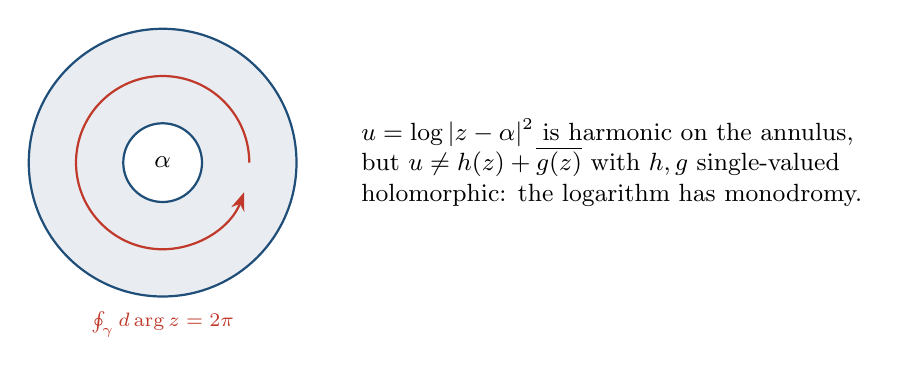
\begin{tikzpicture}
\fill[cA!10] (0,0) circle (1.7); \fill[white] (0,0) circle (0.5);
\draw[cA,thick] (0,0) circle (1.7); \draw[cA,thick] (0,0) circle (0.5);
\node at (0,0) {\small $\alpha$};
\draw[cB,thick,-{Stealth}] (1.1,0) arc (0:340:1.1);
\node[cB,font=\scriptsize] at (0,-2.05) {$\oint_\gamma d\arg z=2\pi$};
\node[align=left,font=\small,anchor=west] at (2.4,0) {$u=\log|z-\alpha|^2$ is harmonic on the annulus,\\ but $u\neq h(z)+\overline{g(z)}$ with $h,g$ single-valued\\ holomorphic: the logarithm has monodromy.};
\end{tikzpicture}
\caption{The Laplacian factors into two Cauchy--Riemann operators, but on an annulus the factor decomposition fails. The obstruction is topological: $H^1_{dR}(\Omega)\neq0$.}\label{f:fig:hole}
\end{figure}

For a fixed $P$ the exact condition is cohomological.

\begin{theorem}[{Cohomological criterion \led{OPF-T4} \pw}]\label{thm:cohom}
Let $\Omega$ be connected, with first Betti number $b_1(\Omega)$. Let $\mathcal N$ be the space of $s$-tuples of global exponential-polynomial solutions with sum zero (dimension $\delta(P)$). The cokernel of the sum map
\[
\Sigma_\Omega:\ \bigoplus_j\ker_{\mathcal A(\Omega)}Q_j\to\ker_{\mathcal A(\Omega)}P
\]
is the kernel of an explicit map $H^1(\Omega;\C)\otimes\mathcal N\to\bigoplus_jH^1(\Omega;\mathcal K_j)$. So the decomposition holds on $\Omega$ iff that map is injective, and
\[
\dimc\operatorname{coker}\Sigma_\Omega\le\delta(P)\;b_1(\Omega).
\]
\dimref{OPF-T4}
\end{theorem}

\begin{example}[{Unique splittings survive holes}]
If $\delta(P)=0$ (disjoint factor curves), the bound gives $\operatorname{coker}\Sigma_\Omega=0$ on \emph{every} connected region, with or without holes. The two parallel transports $\tau-\xi$ and $\tau-\xi-1$ split on an annulus as well.
\end{example}

\subsection{Explicit projectors}

For evolution factors the components are given by a formula. Let
\[
P=\prod_{j=1}^N\big(\tau-a_j(\xi)\big)
\]
with distinct polynomials $a_j$. A component is an eigenfunction of $\partial_t$:
\[
\partial_tu_j=a_j(\partial_x)\,u_j .
\]
Apply $\prod_{k\ne j}(\partial_t-a_k(\partial_x))$ to $u=\sum_lu_l$. Every $u_l$ with $l\ne j$ is killed, because the product contains its own factor. The component $u_j$ is multiplied by $\prod_{k\ne j}(a_j-a_k)(\partial_x)$. Dividing gives the Lagrange formula
\begin{equation}\label{f:eq:lagrange}
u_j=\prod_{k\ne j}\frac{\partial_t-a_k(\partial_x)}{a_j(\partial_x)-a_k(\partial_x)}\;u .
\end{equation}
In Fourier variables the right-hand side is a multiplier that is rational in $\xi$, with poles where two $a_k$ coincide. This is Eq.~\eqref{f:eq:spectral} with the companion matrix replaced by $\partial_t$.

\begin{example}[{Two transports}]
Let $a_1(\xi)=\xi$ and $a_2(\xi)=\xi+1$. The formula gives
\[
u_1=\frac{\partial_t-\partial_x-1}{-1}\,u,\qquad u_2=\frac{\partial_t-\partial_x}{1}\,u .
\]
These are differential operators, with no poles, because $a_1-a_2=-1$ never vanishes: the two lines are disjoint and the splitting is unique.
\end{example}

\begin{proposition}[{Projectors and their poles \led{II-T3, II-T4} \proved}]\label{prop:poly-proj}
The components are obtained by \emph{polynomial} operators if and only if the factor curves are pairwise disjoint, $(Q_i,Q_j)=\ring$. Only factors, not terms, admit projectors that act on one value of $u$ at a time.

\dimref{II-T3}
\end{proposition}

\begin{keypoint}
A ``component'' of $u$ belongs to a \emph{factor} of the symbol, not to a term of the operator. On a region without holes the factor split always exists, and the overlap between components is finite-dimensional and measured exactly by $\delta(P)$. The split by terms fails except on a finite-dimensional space.
\end{keypoint}


% ---- end sections/full_ch6.tex


% ---- begin sections/full_ch7.tex
\section{Regularity of the components}\label{f:ch:regular}
\sectionbrief
{the factor decomposition of Theorem~\ref{f:thm:factor}; $\Omega$ bounded; $u$ in a Sobolev space $H^m(\Omega)$ (square-integrable derivatives up to order $m$).}
{the decomposition is algebraic. To use the components numerically we need them to be as regular as $u$ itself, and to depend continuously on $u$.}
{completes the answer to Q2. It gives the exact condition (a conditioning number $\gamma_N>0$), shows that it can fail, and that the geometry of $\Omega$ against the characteristics decides it. Step~5 of the algorithm checks it.}

\subsection{The pieces can be rougher than the whole}

\begin{falsebox}{Loss of a derivative \led{C12-C1} \falsest}\label{f:cex:loss}
The statement ``if $u\in H^m(\Omega)$ then every component $u_j\in H^m(\Omega)$'' is false. Let $\Omega=(0,1)^2$ and
\[
f=\tau-\xi,\qquad g=\tau-\xi-1 .
\]
For every $m$ there is a smooth $u\in H^m(\Omega)$ with $f(\partial)g(\partial)u=0$ whose unique components $u_1\in\ker f$, $u_2\in\ker g$ are \emph{not} in $H^m$. Exactly one derivative is lost: $u_2=f(\partial)u\in H^{m-1}$.

\dimref{C12-C1}
\end{falsebox}

\begin{intuition}
In the coordinates $s=x+t$ along the characteristics, both factors are first-order ODEs along the same lines, with solutions $1$ and $e^{t}$. On a long chord these two functions are clearly different. Near a corner of the square the chords become arbitrarily short, and on a short chord $1$ and $e^{t}$ are almost collinear. Separating a function into these two shapes then amplifies it by a factor that blows up as the chord shrinks (Figure~\ref{fig:chords}).
\end{intuition}

\begin{figure}[!htb]
\centering
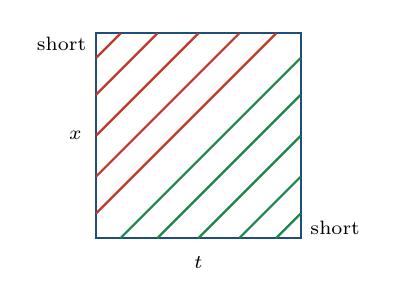
\begin{tikzpicture}[scale=2.6]
\draw[thick,cA] (0,0) rectangle (1,1);
\foreach \s in {0.12,0.3,0.5,0.7,0.88}{
  \draw[cB,thick] ({max(0,-\s+0.0)+0},{\s}) -- ({1-\s},1);}
\foreach \s in {0.12,0.3,0.5,0.7,0.88}{
  \draw[cC,thick] ({\s},0) -- (1,{1-\s});}
\node[font=\scriptsize,anchor=east] at (0,0.95) {short};
\node[font=\scriptsize,anchor=west] at (1,0.05) {short};
\node[font=\scriptsize] at (0.5,-0.12) {$t$};
\node[font=\scriptsize] at (-0.1,0.5) {$x$};
\end{tikzpicture}
\caption{The unit square and the characteristic chords of $\partial_t+\partial_x$. Chords near the corners $(0,1)$ and $(1,0)$ are arbitrarily short. On a short chord the two shapes of the components are nearly collinear, and the splitting is ill-conditioned.}\label{fig:chords}
\end{figure}

\subsection{Two components: the chord criterion}

For two transports in the same direction, the geometry decides everything.

\begin{theorem}[{Chord criterion \led{C12-T3} \proved}]\label{thm:chord}
Let $\Omega$ be bounded, open and convex, $c\in\R$, $d_1\ne d_2$, and
\[
f=\partial_t+c\,\partial_x-d_1,\qquad g=\partial_t+c\,\partial_x-d_2 .
\]
Let $\ell(s)$ be the length of the chord of $\Omega$ along the characteristic line $x-ct=s$, and $\mathcal H_i=\ker_{L^2}f_i$. The following are equivalent:
\begin{enumerate}[label=(\alph*)]
\item the chords do not shrink: $\inf_s\ell(s)>0$;
\item every $u\in L^2$ with $fgu=0$ has components in $L^2$, with
\[
\|u_1\|^2+\|u_2\|^2\le C\,\|u\|^2 ;
\]
\item the sum $\mathcal H_1+\mathcal H_2$ is closed in $L^2$;
\item the Friedrichs cosine of the two spaces is smaller than one, $c_F(\mathcal H_1,\mathcal H_2)<1$.
\end{enumerate}
\dimref{C12-T3}
\end{theorem}

\begin{example}[{Rectangles}]
On a rectangle $I\times J$ with $c\ne0$, the chords in direction $(1,c)$ shrink at two corners. So the global $L^2$ decomposition always fails ($c_F=1$). For $c=0$ the chords are vertical, all of length $|I|$, and the decomposition holds.
\end{example}

\begin{figure}[!htb]
\centering
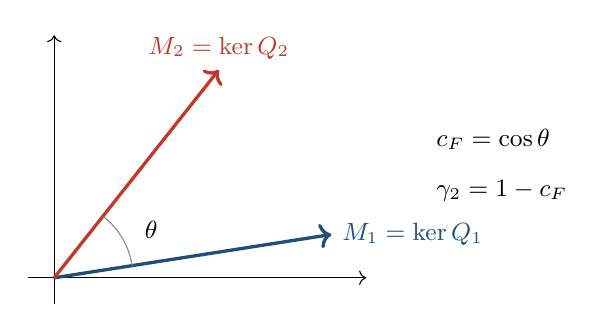
\begin{tikzpicture}[scale=1.1]
\draw[->] (-0.3,0)--(3.6,0); \draw[->] (0,-0.3)--(0,2.8);
\draw[cA,very thick,->] (0,0)--(3.2,0.5) node[right,font=\small]{$M_1=\ker Q_1$};
\draw[cB,very thick,->] (0,0)--(1.9,2.4) node[above,font=\small]{$M_2=\ker Q_2$};
\draw[cG] (0.9,0.14) arc (8.9:51.6:0.9); \node[font=\small] at (1.12,0.55) {$\theta$};
\node[font=\small,anchor=west] at (4.3,1.6) {$c_F=\cos\theta$};
\node[font=\small,anchor=west] at (4.3,1.0) {$\gamma_2=1-c_F$};
\end{tikzpicture}
\caption{The Friedrichs angle $\theta$ between two component spaces. A larger angle means a better-conditioned recovery of the pieces from their sum. As $\theta\to0$ the recovery becomes unstable.}\label{f:fig:friedrichs}
\end{figure}

\subsection{Any number of components}

For $N$ components the right quantity is the conditioning of the sum map
\[
S:\ \bigoplus_{j=1}^N\ker_{H^m}Q_j\to H^m,\qquad S(u_1,\dots,u_N)=\sum_{j=1}^Nu_j .
\]

\begin{definition}[{Conditioning number $\gamma_N$}]\label{def:gamma}
Let $(\ker S)^\perp$ be the tuples orthogonal to the ambiguity of Theorem~\ref{f:thm:factor}. Then
\[
\gamma_N=\inf_{\substack{v\in(\ker S)^\perp\\ v\ne0}}\ \frac{\|Sv\|_{H^m}^2}{\|v\|^2},
\qquad \|v\|^2=\sum_j\|u_j\|_{H^m}^2 .
\]
Equivalently, $\gamma_N$ is the bottom of the spectrum of $S^*S$ on $(\ker S)^\perp$: the square of the smallest nonzero singular value of $S$.
\end{definition}

\begin{intuition}
$\gamma_N$ is the worst ratio between the size of the sum and the size of the pieces. If $\gamma_N>0$, the pieces cannot nearly cancel each other:
\[
\|v\|\le\gamma_N^{-1/2}\,\|Sv\| ,
\]
and recovering them from $u$ is stable. If $\gamma_N=0$, there are large pieces with a tiny sum, and the recovery is unstable. It is exactly the smallest singular value of a least-squares problem.
\end{intuition}

\begin{theorem}[{Regularity criterion \led{C12-P7} \proved}]\label{f:thm:hm}
\begin{enumerate}[label=(\alph*)]
\item Every $u\in\ker_{H^m}P$ has components in $H^m$ if and only if the sum $\sum_j\ker_{H^m}Q_j$ is \emph{closed} and \emph{dense} in $\ker_{H^m}P$.
\item The sum is closed if and only if $\gamma_N>0$. Then the minimal-energy split satisfies, optimally,
\[
\sum_j\|u_j\|_{H^m}^2\le\gamma_N^{-1}\,\|u\|_{H^m}^2 .
\]
\item For $N=2$, $\gamma_2=1-c_F$, the Friedrichs cosine of the two spaces after removing their intersection.
\item For $N\ge3$ the pairwise cosines do not decide. There are three closed subspaces of a Hilbert space with trivial pairwise intersections and closed pairwise sums ($c_F\le\tfrac12$), whose triple sum is not closed.
\end{enumerate}
\dimref{C12-P7}
\end{theorem}

The condition has two parts. Closedness is the conditioning above. Density is a separate question, and on convex regions it is always true.

\begin{theorem}[{Density on convex regions \led{OPF5B-T1} \modulo{H\"ormander, Stein}}]\label{thm:density}
Let $\Omega\subset\R^2$ be bounded and convex. For every operator $P$, every coprime factorisation and every $m\ge0$, the sum $\sum_j\ker_{H^m}Q_j$ is dense in $\ker_{H^m}P$.

\dimref{OPF5B-T1}
\end{theorem}

So on a convex region only $\gamma_N>0$ remains to be checked.

\begin{caution}[title=Added in the complete edition (Phase 10)]
Convexity cannot simply be dropped: on a region with a hole the sum of kernels is \emph{not} dense in general (Proposition~\ref{prop:s10ap1}, the Laplacian on an annulus), and the extension of this theorem to non-convex regions is false. For simply connected Lipschitz regions density was proved in Phase~10 modulo two cited facts (Section~\ref{ch:phase10}).
\end{caution}

\begin{example}[{Cases where the $H^m$ decomposition holds \led{C12-P4} \proved}]
\textbf{$P=\tau\xi$ on a rectangle.} The components are a function of $t$ and a function of $x$. After removing the constants their $H^m$ inner product vanishes, so $c_F=0$ and $\gamma_2=1$.

\textbf{The wave equation on a square.} In characteristic coordinates $s=x+t$, $r=x-t$ the square becomes a rhombus. It can be covered by five pieces on each of which one component is controlled by $u$.

\textbf{Heat and transport on a rectangle} \led{OPR2-T1} \pw. For $P=(\tau-\xi^2)(\tau+c\xi)$ the sum is dense in every $H^m$, so the decomposition holds exactly when $c_F<1$.

The same operator can behave well on one region and badly on another: regularity depends on the \emph{geometry of $\Omega$ against the characteristics}, not on $P$ alone.

\dimref{C12-P4}
\end{example}

\begin{proposition}[{Real transports, $m=0$ \led{OPR2-T2} \pw}]\label{prop:transports}
Let $\Omega$ be convex and bounded, and $Q_j=v_j\cdot\nabla-d_j$ real transports, grouped into classes of parallel directions. Assume that of any two classes at least one has chords bounded below. Then $\sum_j\ker_{L^2}Q_j$ is closed if and only if every class with at least two factors has chords bounded below. In particular, for such transports, closed pairwise sums imply a closed triple sum.

\dimref{OPR2-T2}
\end{proposition}

\begin{caution}[title={Three or more components: what is still open}]
Whether the abstract counterexample of Theorem~\ref{f:thm:hm}(d) can occur for \emph{differential} factors is open in general \openq{} \led{C12-Q2}. Proposition~\ref{prop:transports} rules it out for real transports in $L^2$.
\end{caution}

\begin{keypoint}
Algebraically the split always exists (Theorem~\ref{f:thm:factor}). Analytically the components are as regular as $u$ exactly when the component spaces are separated by a positive angle, $\gamma_N>0$; density is automatic on convex regions. Everything delicate happens at the boundary of $\Omega$ (shrinking chords) or in its topology (holes).
\end{keypoint}


% ---- end sections/full_ch7.tex


% ---- begin sections/full_ch8.tex
\section{Terms inside a factor: the interaction term}\label{f:ch:interaction}
\sectionbrief
{an evolution factor $u_t=Au$ with $A=A_1+\dots+A_N$, the \emph{terms} (advection, diffusion, dispersion, \dots), each a polynomial $a_n(\partial_x)$; flows $S_n(t)=e^{tA_n}$; a bounded rectangle $\Omega$ and a base time $t_0$. The terms commute, except in Section~\ref{f:sec:noncomm}.}
{Proposition~\ref{f:prop:terms} shows that splitting a solution by terms is never exact. Here we compute exactly what is left over, the interaction term $\Eint$, how much it costs, and whether it can be computed stably.}
{third link of the chain, answering Q3. The answer is positive in a function class of exponential type (an exact product formula, cost $O(N)$ per value) and negative in Sobolev spaces (no continuity, no stable regularisation).}

\subsection{From the sum of operators to the interaction term}

The solution of $u_t=Au$ is given by the flow (semigroup) of $A$:
\[
u(t)=e^{tA}u_0=S(t)\,u_0 .
\]
If term $n$ acted alone, it would move the datum to $S_n(t)u_0=e^{tA_n}u_0$, a change of $S_n(t)u_0-u_0$.

The naive guess is that the terms act independently, so that the total change is the sum of the individual changes. It is not: the flow of a sum is not the sum of the flows. For advection ($A_1=-c\partial_x$, a translation) and diffusion ($A_2=D\partial_x^2$, a smoothing), the solution is translated \emph{and} smoothed. This joint action is not ``only translated'' plus ``only smoothed''.

\begin{definition}[{Interaction term}]\label{def:eint}
With $S_n(t)=e^{(t-t_0)A_n}$ the flow of term $n$ alone,
\begin{equation}\label{f:eq:eint-def}
\Eint^{\mathrm{add}}(t)=u(t)-u_0-\sum_{n=1}^N\big(S_n(t)u_0-u_0\big).
\end{equation}
The multiplicative variant compares the true flow with the product of the single flows:
\[
\Eint^{\mathrm{mult}}(t)=e^{(t-t_0)A}-\prod_{n=1}^Ne^{(t-t_0)A_n}.
\]
We write $\Eint$ for $\Eint^{\mathrm{add}}$ unless the distinction matters.
\end{definition}

\subsection{The function class and the exact formula}

Before computing, one must decide on which functions the flows of the single terms are defined. This is not a formality. For the heat equation there are nonzero solutions with zero initial datum (Tychonoff), so ``the diffusion flow of $u_0$'' is not unique without a class.

\begin{definition}[{The class $\Bclass$ of exponential type \led{P1-D1}}]\label{def:B}
For $\rho>0$, $B_\rho(J)$ is the space of smooth $f$ on the interval $J$ with
\[
\|f\|_{B_\rho}^2=\sum_{j\ge0}\rho^{-2j}\,\|f^{(j)}\|_{L^2(J)}^2<\infty .
\]
$\Bclass_\rho(\Omega)$ is the analogous space in $(t,x)$, and $\Bclass=\bigcup_\rho\Bclass_\rho$. Every exponential-polynomial belongs to $\Bclass$, and on $B_\rho$ the derivative is bounded: $\|\partial_x\|\le\rho$.
\end{definition}

On $\Bclass$ every polynomial in $\partial_x$ is a bounded operator, its exponential is an absolutely convergent series, and two such exponentials commute \led{P1-L1, P1-L2} \proved. So the algebra of exponentials of numbers applies to operators.

\begin{theorem}[{Closed form of the interaction \led{P1-T2} \proved}]\label{f:thm:eint}
Let $u\in\Bclass_\rho(\Omega)$ solve $(\partial_t-a(\partial_x))u=0$ with $a=\sum_na_n$, and put
\[
\Delta_n=e^{(t-t_0)a_n(\partial_x)}-\Id .
\]
Then the single flows are unique in $\Bclass$, $\Eint^{\mathrm{mult}}\equiv0$, and
\begin{equation}\label{f:eq:eint}
\Eint^{\mathrm{add}}(t)=\Big[\prod_{n=1}^N(\Id+\Delta_n)-\Id-\sum_{n=1}^N\Delta_n\Big]u_0
=\sum_{|S|\ge2}\ \prod_{n\in S}\Delta_n\,u_0 .
\end{equation}
For a datum $u_0=\sum_kc_ke^{\zeta_kx}$, each mode is multiplied by the number
\[
e_{\ge2}(z)=\prod_n(1+z_n)-1-\sum_nz_n,\qquad z_n=e^{(t-t_0)a_n(\zeta_k)}-1 .
\]
\dimref{P1-T2}
\end{theorem}

\begin{intuition}
Expand the product $\prod_n(\Id+\Delta_n)$. It gives one monomial per subset $S$ of terms. The empty subset gives $\Id$, the singletons give the individual changes $\Delta_n$, and everything else is interaction. So the interaction is the sum of products of \emph{at least two} increments: it appears only when at least two terms act together.

For two terms the formula is simply
\[
\Eint=\Delta_1\Delta_2\,u_0=(S_1-\Id)(S_2-\Id)\,u_0 .
\]
In each Fourier mode, the interaction is the product of the two single-term responses.
\end{intuition}

\begin{example}[{Advection--diffusion with a Gaussian datum}]\label{ex:advdiff}
Take $u_t=-cu_x+Du_{xx}$ and $u_0=g(x;\sigma^2)$, where
\[
g(x;v)=\frac{e^{-x^2/2v}}{\sqrt{2\pi v}} .
\]
The two flows are a translation and a Gaussian smoothing:
\[
S_1u_0=g(x-ct;\sigma^2),\qquad S_2u_0=g(x;s^2),\qquad u=g(x-ct;s^2),
\]
with $s^2=\sigma^2+2Dt$. The interaction term is
\[
\Eint=g(x-ct;s^2)-g(x-ct;\sigma^2)-g(x;s^2)+g(x;\sigma^2).
\]
Figure~\ref{f:fig:eint}(a) shows that it is comparable in size to $u$ itself: it is not a small correction. In Fourier variables
\[
\frac{|\widehat{\Eint}(\kappa)|}{|\hat u_0(\kappa)|}=\big|e^{-ic\kappa t}-1\big|\cdot\big|e^{-D\kappa^2t}-1\big|\le2 .
\]
It vanishes at $\kappa=0$ and whenever $c\kappa t\in2\pi\Z$, where the translation returns to the identity.
\end{example}

\begin{figure}[!htb]
\centering
\begin{tikzpicture}
\begin{axis}[width=7.4cm,height=5.6cm,xlabel={$x$},xmin=-6,xmax=8,ymin=-0.2,ymax=0.45,
 title={\small (a) $t=1$, $c=2$, $D=\tfrac12$},legend style={font=\scriptsize,draw=none,fill=white,fill opacity=0.8,text opacity=1,at={(0.02,0.98)},anchor=north west},
 domain=-6:8,samples=140,no markers]
\addplot[cG,thick,dashed] {gauss(x,1)};
\addplot[cA,thick] {gauss(x-2,2)};
\addplot[cB,very thick] {gauss(x-2,2)-gauss(x-2,1)-gauss(x,2)+gauss(x,1)};
\legend{$u_0$,$u(t)$,$\Eint$}
\end{axis}
\end{tikzpicture}\hfill
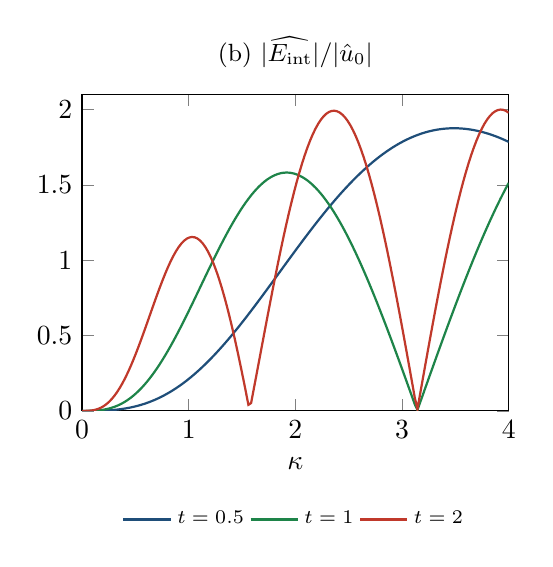
\begin{tikzpicture}
\begin{axis}[width=7.0cm,height=5.6cm,xlabel={$\kappa$},xmin=0,xmax=4,ymin=0,ymax=2.1,
 title={\small (b) $|\widehat{\Eint}|/|\hat u_0|$},legend style={font=\scriptsize,draw=none,at={(0.5,-0.28)},anchor=north,legend columns=3},
 domain=0:4,samples=160,no markers]
\addplot[cA,thick] {sqrt(((cos(deg(2*0.5*x))-1)^2+sin(deg(2*0.5*x))^2)*(exp(-0.5*0.5*x^2)-1)^2)};
\addplot[cC,thick] {sqrt(((cos(deg(2*1.0*x))-1)^2+sin(deg(2*1.0*x))^2)*(exp(-0.5*1.0*x^2)-1)^2)};
\addplot[cB,thick] {sqrt(((cos(deg(2*2.0*x))-1)^2+sin(deg(2*2.0*x))^2)*(exp(-0.5*2.0*x^2)-1)^2)};
\legend{$t=0.5$,$t=1$,$t=2$}
\end{axis}
\end{tikzpicture}
\caption{Advection--diffusion with Gaussian datum ($\sigma^2=1$). (a) The datum, the solution and the interaction term. (b) The Fourier ratio of the interaction to the datum, for three times.}\label{f:fig:eint}
\end{figure}

\begin{example}[{A stationary state is pure interaction}]
For advection--diffusion, a stationary solution satisfies $-cu_x+Du_{xx}=0$, for example $u=e^{cx/D}$. The full flow leaves it unchanged, so $u(t)-u_0=0$. The single flows do change it, and the interaction term exactly cancels their changes. In this mode
\[
\Eint=-4\sinh^2\!\Big(\frac{\theta}{2}\Big)\,u,\qquad \theta=\frac{c^2(t-t_0)}{D}.
\]
Equilibrium is the case where all the dynamics is interaction.
\end{example}

\subsection{Cost: $O(N)$ versus $2^N$}

Expanding~\eqref{f:eq:eint} produces one monomial per subset with at least two elements: $2^N-N-1$ cross terms (Figure~\ref{f:fig:lattice}). Writing the \emph{complete table} of cross terms is therefore exponential. Computing one \emph{value} is cheap, because the product is never expanded.

\begin{figure}[!htb]
\centering
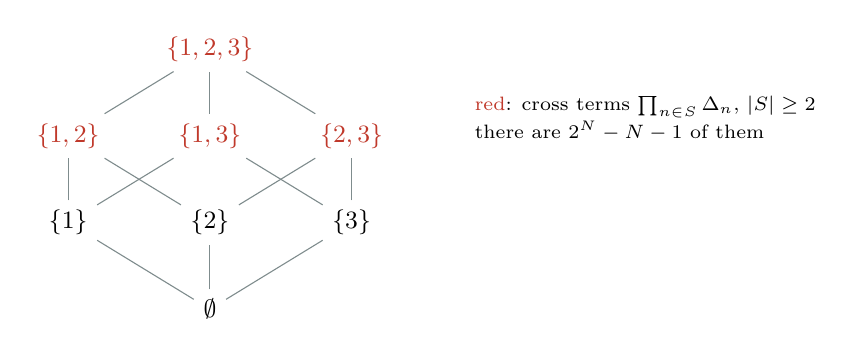
\begin{tikzpicture}[x=1.8cm,y=1.1cm,every node/.style={font=\small}]
\node (e) at (0,0) {$\emptyset$};
\node (1) at (-1,1) {$\{1\}$}; \node (2) at (0,1) {$\{2\}$}; \node (3) at (1,1) {$\{3\}$};
\node[text=cB] (12) at (-1,2) {$\{1,2\}$}; \node[text=cB] (13) at (0,2) {$\{1,3\}$}; \node[text=cB] (23) at (1,2) {$\{2,3\}$};
\node[text=cB] (123) at (0,3) {$\{1,2,3\}$};
\foreach \a/\b in {e/1,e/2,e/3,1/12,1/13,2/12,2/23,3/13,3/23,12/123,13/123,23/123} \draw[cG] (\a)--(\b);
\node[anchor=west,align=left,font=\scriptsize] at (1.8,2.2) {\textcolor{cB}{red}: cross terms $\prod_{n\in S}\Delta_n$, $|S|\ge2$\\ there are $2^N-N-1$ of them};
\end{tikzpicture}
\caption{The subset lattice for $N=3$ terms. Each node with at least two elements is one cross term of the interaction.}\label{f:fig:lattice}
\end{figure}

\begin{theorem}[{Cost of the interaction \led{P1-T3} \proved}]\label{thm:cost}
Let the datum be a sum of $M$ exponentials with polynomial prefactors of degree at most $L$, and let $d_n=\deg a_n$.
\begin{enumerate}[label=(\alph*)]
\item One value of $\Eint$ costs
\[
O\Big(M\big[N(L+1)^2+(L+1)\textstyle\sum_n(d_n+1)\big]\Big);
\]
for simple exponentials ($L=0$) this is $O\big(M(N+\sum_nd_n)\big)$: linear in the number of terms.
\item All aggregates by order, $E^{(k)}=\sum_{|S|=k}\prod_{n\in S}\Delta_nu_0$ for $2\le k\le N$, cost $O(MN^2(L+1)^2)$ plus the same term in $d_n$.
\item The full table of cross terms has $M(2^N-N-1)$ entries and costs $\Theta\big(M\,2^N(L+1)^2\big)$.
\end{enumerate}
\dimref{P1-T3}
\end{theorem}

\begin{example}[{Counting operations for one mode}]
For one simple mode $e^{\zeta x}$ and $N$ terms, compute the $N$ numbers $z_n=e^{(t-t_0)a_n(\zeta)}-1$, then the product $\prod_n(1+z_n)$ with $N-1$ multiplications, then subtract $1+\sum_nz_n$. That is about $3N$ operations. Listing the $2^N-N-1$ products $\prod_{n\in S}z_n$ one by one costs $2^N$ times more for large $N$: already for $N=20$, about a million.
\end{example}

\subsection{The flows are not determined without a class}

\begin{proposition}[{Non-uniqueness of single flows \led{P1-P1(a)--(d)} \proved}]\label{prop:nonuniq}
On a bounded rectangle, without a function class:
\begin{enumerate}[label=(\alph*)]
\item for the transport term $a_n=\xi$, the flow of a datum is any smooth extension of it: infinitely many choices;
\item for the diffusion term $a_n=\xi^2$, there are nonzero heat solutions with zero datum (Tychonoff) \cf;
\item so $\Eint$ is not a function of $u$ alone; inside $\Bclass$ it is unique.
\end{enumerate}
\dimref{P1-P1}
\end{proposition}

\subsection{Stability: the interaction cannot be computed stably}

\begin{theorem}[{No continuous extension to Sobolev spaces \led{P1-P1(e)} \falsest}]\label{f:thm:nocont}
Let $Q=\tau+c\xi-D\xi^2$ with $c,D>0$ (advection--diffusion), terms $a_1=-c\xi$ and $a_2=D\xi^2$, and any base time $t_0$. For every $m$,
\[
\sup\Big\{\frac{\|\Eint\|_{L^2(\Omega)}}{\|u\|_{H^m(\Omega)}}:\ u\in\EP,\ Qu=0,\ u\ne0\Big\}=\infty .
\]
So $u\mapsto\Eint$ does not extend continuously from exponential-type data to $H^m$, although exponential-type data are dense. The same holds for every evolution with at least two non-proportional terms; for proportional terms the interaction is continuous \led{OPA-P3} \proved.

\dimref{P1-P1e}
\end{theorem}

\begin{intuition}
On a bounded interval, a real exponential $e^{\zeta x}$ with large $\zeta$ is a legitimate datum. The diffusion flow alone amplifies it by $e^{D\zeta^2t}$. The true solution is only changed by the factor $e^{(D\zeta^2-c\zeta)t}$ times the datum norm. The interaction term must cancel the gap, and the gap grows faster than any Sobolev norm of the datum.
\end{intuition}

This instability has three consequences for any algorithm that wants to be stable.

\begin{theorem}[{No regularisation removes the interaction \led{P2-T1, P2-T2, P2-T4} \proved}]\label{f:thm:noreg}
\begin{enumerate}[label=(\alph*)]
\item \textbf{Any penalty leaves the same residual.} For any regulariser (an $\ell^1$ sparsity penalty, $\ell^2$, total variation, \dots) the residual of the best fit converges to the distance of $u$ from the closed span of the per-term pieces.
\item \textbf{Inside an evolution factor that residual is large.} If no single term exhausts the symbol, the part of $u$ outside the span of the per-term kernels satisfies
\[
\|E^\perp(u)\|_{H^m}\ \ge\ \frac{\|g(\partial_x)u\|_{H^{m-k}}}{C},\qquad g=\prod_n(a-a_n).
\]
Only a finite-dimensional space of exponential-polynomials has a per-term representation. For advection--diffusion it is
\[
\spn\{1,\ x-ct,\ (x-ct)^2+2Dt\}.
\]
\item \textbf{No uniformly Lipschitz regularisation exists.} Any family of Lipschitz maps converging pointwise to an unbounded map has Lipschitz constants tending to infinity. Every exact selection of components has Lipschitz constant at least $\gamma_N^{-1/2}$.
\end{enumerate}
\dimref{P2-T2}
\end{theorem}

\begin{caution}[title=Added in the complete edition (Phase 10)]
The instability above is proved for advection--diffusion. The general statement ``for every operator with at least two non-proportional terms'' (P1-Q6) is false as written: with constant terms, for example reaction--diffusion, the interaction is continuous from $H^1$. The correct dichotomy is by the number of terms of degree $\ge1$ (Theorem~\ref{thm:s10at1}, Section~\ref{ch:phase10}).
\end{caution}

\begin{aside}{The one continuous split found}
A \emph{balance} decomposition of $u$ writes each term's contribution as the time integral of that term applied to the true solution:
\[
u^{(i)}(t)=\int_{t_0}^{t}a_i(\partial_x)\,u(s)\dd s .
\]
It is exact ($u-u_0=\sum_iu^{(i)}$) and continuous in $H^m$ \led{P3-T6} \pw. But it needs an external principle to decide that this is ``the'' contribution of term $i$: it uses the full solution, not the flow of the term alone.
\end{aside}

\subsection{Time-dependent perturbation theory}

The product formula needs commuting terms. With non-commuting terms, or with boundary conditions, there is no closed formula, but $\Eint$ is still defined by~\eqref{f:eq:eint-def}. Perturbation theory expands the flow in powers of the interaction. Split $A=A_1+B$, where $A_1$ is the principal term and $B$ the rest. The Dyson--Phillips series is
\begin{equation}\label{f:eq:dyson}
\begin{aligned}
S(t)&=\sum_{k\ge0}S^{(k)}(t),\\
S^{(0)}(t)&=e^{tA_1},\\
S^{(k+1)}(t)&=\int_0^te^{(t-s)A_1}\,B\,S^{(k)}(s)\dd s .
\end{aligned}
\end{equation}
$S^{(k)}$ collects the histories in which $B$ acts $k$ times, at intermediate times, with the flow of $A_1$ in between. This is the interaction picture of quantum mechanics~\cite{dy}.

\begin{theorem}[{Dyson--Phillips converges for every time \led{P3-T1} \proved}]\label{thm:dyson}
Let $A_1=a(\partial_x)$ with symbol of degree $q$, and $B=\sum_{k\le r}b_k(x)\partial_x^k$ with bounded coefficients and $r<q$. The symbol condition
\[
\mathrm{Re}\,a(i\kappa)\le\omega-\delta|\kappa|^q\qquad(\delta>0)
\]
holds if and only if $q$ is even and the leading coefficient has negative real part (a dissipative operator of even order). Under it, the Dyson--Phillips series converges in operator norm, uniformly on every bounded time interval, and its sum is the semigroup generated by $A_1+B$. The same holds with Dirichlet conditions on an interval.

\dimref{P3-T1}
\end{theorem}

So $\Eint$ is well defined and can be approximated by truncating the series even without a closed formula.

\begin{proposition}[{Interaction created by a boundary \led{P1-P6, P3-T3, OPA-T2, OPF5A-T5} \proved}]\label{prop:boundary}
On an interval with Dirichlet conditions, advection and diffusion no longer commute: the boundary creates an $\Eint^{\mathrm{mult}}$ already at first order \led{P1-P6}. For small times its size is governed by how the datum touches the boundary. If $k$ is the order of contact (the first nonvanishing derivative of $u_0$ at the endpoints), then
\[
\|\Eint^{\mathrm{mult}}(t)\|=\Theta\big(t^{k/2+3/4}\big)\qquad(t\to0).
\]
For compatible data the leading constant is explicit and proportional to
\[
|c|\,\frac{\tilde N_k}{k!}\,D^{k/2-1/4}\sqrt{u_0^{(k)}(0)^2+u_0^{(k)}(L)^2}.
\]
\dimref{OPF5A-T5}
\end{proposition}

The smoother the datum is against the boundary, the faster the boundary interaction becomes negligible as $t\to0$.

\subsection{Non-commuting terms}\label{f:sec:noncomm}

If two terms do not commute, the flow of their sum is not the product of the flows. By the Baker--Campbell--Hausdorff formula,
\[
e^{tA_1}e^{tA_2}=\exp\Big(t(A_1+A_2)+\frac{t^2}{2}[A_1,A_2]+O(t^3)\Big).
\]
The commutators generate a Lie algebra, and its type decides what can be done.

\begin{theorem}[{Lie-algebra classification \led{P1-T4, P1-P5, P1-T5} \proved}]\label{f:thm:lie}
\begin{enumerate}[label=(\alph*)]
\item \textbf{Finite and solvable.} An exact formula exists, with $d=\dim\mathfrak g$ entire scalar functions (Wei--Norman). Example: $\partial_x^2+x$, and the Ornstein--Uhlenbeck operator.
\item \textbf{Finite, not solvable} (for example $\mathfrak{sl}_2$). A closed form exists locally in time; it can fail globally.
\item \textbf{Infinite adjoint orbit.} If $X$ and all the iterated commutators $\mathrm{ad}_X^kY$ are linearly independent (for example $X=x^a\partial_x$, $Y=\partial_x$ with $a\ge3$), then no finite product of flows of the two terms, with times analytic in $t$ and in the coupling $\varepsilon$ and with the flows of $Y$ switched off at $\varepsilon=0$, reproduces $e^{t(X+\varepsilon Y)}$. Only series expansions exist.
\end{enumerate}
\dimref{P1-T5}
\end{theorem}

\begin{example}[{Which potentials allow Wei--Norman}]
For $i\partial_t=-\partial_x^2+V(x)$, the operators $\partial_x^2$ and $x^2$ generate the finite Lie algebra $\mathfrak{sl}_2$: the harmonic oscillator has a closed-form evolution. With $V=x^3$, repeated commutators produce polynomials of ever higher degree and the algebra is infinite-dimensional. But the hypothesis of part (c) fails there, so whether a finite product of flows is impossible for $\partial_x^2$ and $x^k$ with $k\ge3$ is still \openq{} \led{P1-Q3}. Part~(c) applies to the transport with polynomial speed $u_t=(x^a+\varepsilon)u_x$, $a\ge3$, which nevertheless has an explicit solution by characteristics: the theorem excludes only a factorisation into flows of the terms.
\end{example}

\begin{caution}[title={Other ways commutativity is lost}]
\begin{itemize}
\item \textbf{Repeated factors.} For $(\tau-a)^e$ the ``multiplicity term'' is a nilpotent shift. It commutes with the other terms, its flow is polynomial in time (secular growth), and $\Eint^{\mathrm{mult}}=0$ \led{OPF-T2} \pw.
\item \textbf{Second-order evolutions} (wave, Klein--Gordon). The companion blocks do not commute, so the first-order calculus fails; a Gauss factorisation works mode by mode \led{II-T7, P1-P4} \proved.
\end{itemize}
\end{caution}

\begin{keypoint}
For commuting terms the interaction is explicit and cheap to evaluate, but it can be neither removed nor computed stably in Sobolev spaces. That instability is not a defect of the formula: it is a property of the question. For non-commuting terms even the explicit form is lost, except when the terms generate a finite solvable Lie algebra.
\end{keypoint}


% ---- end sections/full_ch8.tex


% ---- begin sections/full_ch9.tex
\section{Nonlinear equations}\label{f:ch:nonlin}
\sectionbrief
{a scalar evolution in one space variable, $u_t=\sum_nT_n(u)$, each term $T_n$ linear or polynomial in the jet $(u,u_x,u_{xx},\dots)$; a smooth datum $u_0$; the exact solution is known. Benchmarks: viscous Burgers, KdV--Burgers, Fisher--KPP; KdV and NLS as integrable controls.}
{for a nonlinear equation the single-term flows do not commute and superposition fails. ``Component per term'' needs a new definition, and identification needs a new frame (a dictionary). We give both and compute them where everything is explicit.}
{fourth link of the chain. It reuses the earlier chapters through the jet expansion and the annihilator idea. Its results are weaker and relative, but sharp on the benchmark models.}

\subsection{The interaction term for nonlinear flows}

Let $S_n^t$ be the flow of $u_t=T_n(u)$ alone, which is now a nonlinear map. Definition~\eqref{f:eq:eint-def} still makes sense:
\[
\Eint(t)=u(t)-u_0-\sum_n\big(S_n^tu_0-u_0\big).
\]
There is no product formula, because the flows do not commute. But the Taylor expansion in time is explicit.

\begin{theorem}[{Jet of the nonlinear interaction \led{S4T-T1} \proved}]\label{f:thm:jet}
For smooth data,
\[
\Eint(t)=\frac{t^2}{2}\sum_{n\ne m}T_n'[u_0]\big(T_m(u_0)\big)+O(t^3),
\]
where $T_n'[u_0](v)$ is the derivative (Fr\'echet derivative) of $T_n$ at $u_0$ in the direction $v$.

\dimref{S4T-T1}
\end{theorem}

\begin{intuition}
To first order in $t$ every flow moves $u_0$ by $t\,T_n(u_0)$, and these moves add exactly: there is no interaction at order $t$. At order $t^2$ the full flow sees each term react to the motion caused by the others. That reaction is the derivative of $T_n$ in the direction of $T_m(u_0)$.
\end{intuition}

\begin{example}[{Burgers}]\label{f:ex:burgers-jet}
For $u_t=-uu_x+\nu u_{xx}$ take $T_1(u)=-uu_x$ and $T_2(u)=\nu u_{xx}$. The derivatives are
\[
T_1'[u](v)=-(vu_x+uv_x),\qquad T_2'[u](v)=\nu v_{xx}.
\]
Substituting the other term:
\begin{align*}
T_1'[u_0]\big(T_2(u_0)\big)&=-\nu\,\big(u_0''u_0'+u_0u_0'''\big),\\
T_2'[u_0]\big(T_1(u_0)\big)&=-\nu\,\big(3u_0'u_0''+u_0u_0'''\big).
\end{align*}
Half the sum, times $t^2$, gives
\[
\Eint(t)=-\nu\,\big(u_0u_0'''+2u_0'u_0''\big)\,t^2+O(t^3).
\]
\end{example}

\subsection{Before, at and after the shock}

The flow of the single term $-uu_x$ (inviscid Burgers) forms shocks: along each characteristic $u$ is constant and the characteristic moves with speed $u$, so faster parts overtake slower ones. For $u_0=\sin x$ the characteristics are
\[
x=\xi+t\sin\xi,
\]
and since
\[
\frac{\partial x}{\partial\xi}=1+t\cos\xi
\]
first vanishes at $\xi=\pi$, the breaking time is $t^*=1$ (Figure~\ref{f:fig:burgers}).

\begin{figure}[!htb]
\centering
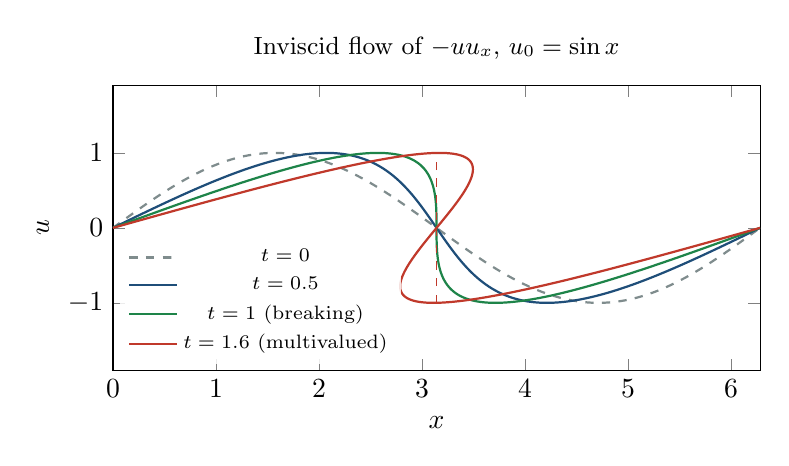
\begin{tikzpicture}
\begin{axis}[width=9.8cm,height=5.2cm,xlabel={$x$},ylabel={$u$},xmin=0,xmax=6.283,ymin=-1.9,ymax=1.9,
 legend style={font=\scriptsize,draw=none,fill=white,fill opacity=0.85,text opacity=1,at={(0.01,0.02)},anchor=south west},
 title={\small Inviscid flow of $-uu_x$, $u_0=\sin x$},no markers,domain=0:6.283185,samples=200,smooth]
\addplot[cG,thick,dashed,variable=\z] ({\z},{sin(deg(\z))});
\addplot[cA,thick,variable=\z] ({\z+0.5*sin(deg(\z))},{sin(deg(\z))});
\addplot[cC,thick,variable=\z] ({\z+1.0*sin(deg(\z))},{sin(deg(\z))});
\addplot[cB,thick,variable=\z] ({\z+1.6*sin(deg(\z))},{sin(deg(\z))});
\draw[cB,dashed] (axis cs:3.14159,-1) -- (axis cs:3.14159,1);
\legend{$t=0$,$t=0.5$,$t=1$ (breaking),$t=1.6$ (multivalued)}
\end{axis}
\end{tikzpicture}
\caption{At $t=1$ the profile has a vertical tangent and the gradient blows up. Beyond that the curve folds; the physical (entropy) solution replaces the fold by a jump at $x=\pi$. This breaking is what makes the interaction term discontinuous after the shock.}\label{f:fig:burgers}
\end{figure}

The interaction changes qualitatively with time, and each regime needs different tools.

\subsubsection{Before the shock: a closed form}

\begin{theorem}[{Closed form before the shock \led{S4T-T2, S4T-P3} \proved}]\label{thm:preshock}
For Burgers with $t<t^*$, the interaction term has a closed form at first order in the viscosity, with remainder
\[
O\big(\nu^2\varepsilon^2t^3\big),
\]
where $\varepsilon$ measures the size of the datum. The closed form blows up at the breaking time $t^*$.

\dimref{S4T-T2}
\end{theorem}

The tool is the Cole--Hopf substitution
\[
u=-2\nu\,\frac{\varphi_x}{\varphi},
\]
which turns Burgers into the heat equation $\varphi_t=\nu\varphi_{xx}$~\cite{ch}. It plays the role of an ``exact linearisation''. For KdV and NLS the inverse scattering transform plays the same role.

The analyticity radius of the Burgers solution with datum $U_0$ is at least $2/\mathrm{osc}(U_0)$, and this bound is optimal \led{F4L-P3} \proved.

\subsubsection{After the shock: sizes in $L^1$}

The flow of $-uu_x$ alone forms a shock, so $\Eint$ has jumps whose size does not depend on $\nu$ \led{S4T-T3} \modulo{[F1]}. This is forced by the definition. A function with a jump is not in $H^1$, so Sobolev norms are no longer the right measure. Pointwise values are unreliable, but the \emph{measure} of the discrepancy is well behaved. The meaningful sizes are in $L^1$.

\begin{theorem}[{Interaction after the shock \led{OPA-T1} \modulo{Kru\v zkov}}]\label{thm:shock}
At a fixed time $t>t^*$, under a nondegeneracy condition $(H_t)$ that holds for example for $u_0=\sin x$,
\[
\|\Eint(t)\|_{L^1}=\Theta(\nu)\qquad(\nu\to0).
\]
Each shock of strength $\rho$ contributes
\[
4\nu\log\big(2\cosh(\rho/2)\big)
\]
to the leading term.

\dimref{OPA-T1}
\end{theorem}

\begin{theorem}[{Uniform rate across the shock time \led{OPF5A-T1, OPF5A-T2} \modulo{Kru\v zkov}}]\label{thm:uniform}
Uniformly in time, near the shock time,
\[
\|\Eint(t)\|_{L^1}\approx2\nu\log\frac{1}{\max(|t-t^*|,\nu)}+O(\nu),
\]
so that
\[
\sup_{t\le T}\|\Eint(t)\|_{L^1}=\nu|\log\nu|+O(\nu),
\]
with leading coefficient exactly $1$. The constant at the shock time is explicit (it involves the Pearcey constant $1.188654\ldots$). For data with several shock births the uniform rate is \condl{} on a localisation lemma.

\dimref{OPF5A-T2}
\end{theorem}

\begin{proposition}[{The splitting error is larger \led{OPF5D-T6} \proved}]\label{prop:splitting}
The error of the splitting scheme ``advection, then diffusion'' is
\[
\|S(t)u_0-S_2^tS_1^tu_0\|_{L^1}=\Theta\big(\sqrt\nu\big),
\]
larger than the interaction term itself. Treating the terms one after the other costs more than ignoring their interplay.

\dimref{OPF5D-T6}
\end{proposition}

\begin{table}[!htb]
\centering\small
\begin{tabular}{@{}L{3.0cm}L{4.8cm}L{6.4cm}@{}}
\toprule
Regime & What happens & Tools and results\\\midrule
before, $t<t^*$ & smooth; characteristics do not cross & jet (Thm.~\ref{f:thm:jet}), closed form (Thm.~\ref{thm:preshock}), Cole--Hopf\\
at breaking, $t=t^*$ & the gradient blows up & smoothness estimates fail; the closed form blows up\\
after, $t>t^*$ & the single-term flow has a jump & $L^1$: $\Theta(\nu)$, uniform $\nu|\log\nu|$, splitting $\Theta(\sqrt\nu)$\\
\bottomrule
\end{tabular}
\caption{The three regimes of the Burgers interaction term.}\label{f:tab:regimes}
\end{table}

\subsection{Identification relative to a dictionary}

Nonlinear terms cannot be handled by the ideal $\Ann(u)$: there is no ring of operators. Instead one fixes a finite list of candidates.

\begin{notebox}{Dictionary setting}
\begin{itemize}
\item A \emph{dictionary} $\mathcal D$ is a finite set of monomials in the jet $(u,u_x,u_{xx},\dots)$ of degree at most $d$ and order at most $k$, for example $\{u,\ u_x,\ uu_x,\ u_{xx},\ u_{xxx}\}$. $V=\spn\mathcal D$.
\item $I(u)$ is the set of all differential polynomial relations that $u$ satisfies.
\item $[F]$ is the differential ideal generated by the equation $F$: $F$, its derivatives $\partial_xF,\partial_tF,\dots$, and their combinations.
\item $\mathcal J_u$ is a jet-level obstruction defined from $u$, and $\psi$ maps the dictionary into the jet space.
\end{itemize}
\end{notebox}

\begin{theorem}[{Dictionary criterion \led{S4ID-T1} \proved}]\label{f:thm:dict}
For smooth $u$ on any $\Omega$ there is an exact sequence
\[
0\to[F]\cap V\to I(u)\cap V\to\mathcal J_u\cap\psi(V)\to0 .
\]
In particular
\[
I(u)\cap V=[F]\cap V\iff\mathcal J_u\cap\psi(V)=0 .
\]
\dimref{S4ID-T1}
\end{theorem}

The correct statement is therefore ``the relations are exactly $F$ \emph{modulo its differential consequences}''. The literal statement $I(u)\cap V=\spn\{F\}$ is false in complete dictionaries, because they contain $\partial_xF$ \led{S4ID-P1} \proved.

\begin{theorem}[{Burgers with $N$ shocks \led{S4ID-T2, OP-T7} \proved}]\label{thm:burgersN}
For the $N$-shock solutions of Burgers, $u$ identifies its equation in the evolutionary dictionary with $d$ unknown terms if and only if $d\le N$.

\dimref{S4ID-T2}
\end{theorem}

\begin{example}[{One shock, two unknowns}]
The travelling front $u=-\tanh(x/(2\nu))$ is a $1$-shock solution. It satisfies Burgers, but also the ODE that every travelling wave satisfies. With $d=2$ unknown coefficients (in front of $uu_x$ and $u_{xx}$) and $N=1$, the theorem says $u$ does not identify the pair. It fixes only their ratio.
\end{example}

\begin{theorem}[{KdV $N$-solitons \led{S4ID-T3, OPF5C-T2} \modulo{Novikov 1974}}]\label{thm:kdv}
For the $N$-soliton solution of KdV, the annihilator in the jet variables is principal, generated by one polynomial $\Pi_N$ of total degree
\[
\deg\Pi_N=(N+2)\,2^{N-1}.
\]
For generic $N=2$ this degree is $8$. The solution identifies KdV in a dictionary of degree $d$ if and only if $d<(N+2)2^{N-1}$.

\dimref{OPF5C-T2}
\end{theorem}

\begin{proposition}[{A closed form does not identify \led{S4ID-T4} \proved}]
If $u$ has a closed form, it lives on a smaller variety and satisfies extra relations: it does not identify its equation in a complete dictionary.

\dimref{S4ID-T4}
\end{proposition}

This is the nonlinear analogue of ``exponential-polynomials never identify''.

\subsection{Integrable models and scattering}

\begin{itemize}
\item \textbf{Hirota $N$-solitons.} The interaction is pairwise and localised: it is determined by pairs of solitons, integrates to $0$, and costs $O(N^3)$ \led{INT-P5, INT-P6} \proved.
\item \textbf{Scattering identification.} For reflectionless KdV, Novikov's centraliser characterises the potential \led{INT-T1, OPF5D} \proved. For NLS with multiplicity, identification by the scattering data holds; without multiplicity it is \falsest. The Lax and zero-curvature relations hold for all $n$ \led{OP-P17, OP-P18} \proved.
\item \textbf{KdV--Burgers.} The jet is proved. Before the shock the dispersive correction has remainder $O\big((\nu+|\delta|)^2\big)$ \led{OPR2-T5} \modulo{local well-posedness}.
\item \textbf{Fisher--KPP.} Only a jet-level statement with an estimate that is not uniform in time \led{S4T-P5} \proved. No sharp analogue of the Burgers asymptotics is claimed.
\end{itemize}

\begin{caution}[title={Open in the nonlinear part}]
For analytic KdV data with nonzero reflection, is there an autonomous ODE in $x$? Three obstructions are proved, among them the cubic relation of Airy \openq{} \led{INT-Q1}. The exact minimal syzygy degrees $\delta_N(K)$ are known in nine computer-assisted cases; their general formulas are conjectures \openq{} \led{OPF5C-Q1}.
\end{caution}

\subsection{Linear versus nonlinear}

\begin{table}[!htb]
\centering\small
\begin{tabular}{@{}L{3.0cm}L{5.8cm}L{5.8cm}@{}}
\toprule
 & Linear (Sections~\ref{f:ch:algebra}--\ref{f:ch:interaction}) & Nonlinear (this chapter)\\\midrule
Candidate equations & the ring $\ring=\C[\tau,\xi]$ & a finite dictionary $V=\spn\mathcal D$\\
Relations of $u$ & the ideal $\Ann(u)$ & the differential ideal $I(u)$\\
What $P$ generates & the principal ideal $(P)$ & the differential ideal $[F]$\\
Identification & $\Ann(u)=(P)$ & $I(u)\cap V=[F]\cap V$\\
What escapes & the point spectrum $\Var(J_u)$ & the obstruction $\mathcal J_u\cap\psi(V)$\\
Solutions that never identify & exponential-polynomials & closed forms\\
Interaction & product formula, $O(N)$ & $t^2$ jet; $\Theta(\nu)$, $\nu|\log\nu|$ after shocks\\
\bottomrule
\end{tabular}
\caption{The linear and nonlinear problems side by side.}\label{f:tab:lin-nonlin}
\end{table}

\begin{keypoint}
Nonlinearity changes the objects (single-term flows with shocks, dictionaries instead of rings) but not the question. Where the formula is closed (before the shock, solitons) the answer is explicit. Across a shock the interaction does not vanish with the viscosity: it shrinks like $\nu|\log\nu|$.
\end{keypoint}


% ---- end sections/full_ch9.tex


% ---- begin sections/full_ch10.tex
\section{The algorithm}\label{ch:algo}
\sectionbrief
{an input in one of the data models M1--M3 (Section~\ref{f:ch:data}) and, for each step, the hypotheses of the theorem that justifies it.}
{to turn the theorems into one procedure with explicit inputs, outputs and guarantees.}
{operational summary of Sections~\ref{f:ch:ident}--\ref{f:ch:nonlin}. Table~\ref{tab:steps} lists the steps, Figure~\ref{fig:algo} gives the control flow, and two worked examples make every step concrete.}

\subsection{The pipeline}

\begin{center}\small
\begin{tabular}{@{}c L{2.6cm} L{5.0cm} L{5.4cm}@{}}
\toprule
Step & Task & Result relied upon & Output\\\midrule
0 & Input & data models M1--M3 & exact $u$\\
1 & Annihilator & Gram matrix of a dictionary & a candidate $P$\\
2 & Factor & unique factorisation (F1) & factors $P_i$, multiplicities $e_i$\\
3 & EP test & Lemma~\ref{f:lem:ep}, Thm.~\ref{f:thm:ident}, Ch.~\ref{f:ch:data} & a verdict per factor\\
4 & Reduce & Thms.~\ref{thm:spec} and~\ref{thm:intrinsic} & $G_u$, $J_u$, certificate\\
5 & Decompose & Thm.~\ref{f:thm:factor}, Eq.~\eqref{f:eq:lagrange}, Thm.~\ref{f:thm:hm} & components $u_j$, ambiguity $\delta(P)$, check $\gamma_N$\\
6 & Terms & Thms.~\ref{f:thm:eint}, \ref{thm:cost}, \ref{f:thm:lie} & log-symbol, $\Eint$\\
7 & Nonlinear branch & Thms.~\ref{f:thm:dict}, \ref{f:thm:jet} & relative identification, flow-based $\Eint$\\
\bottomrule
\end{tabular}
\captionof{table}{The steps of the algorithm: what each step does, which result justifies it, and what it returns.}\label{tab:steps}
\end{center}

\begin{figure}[!htb]
\centering
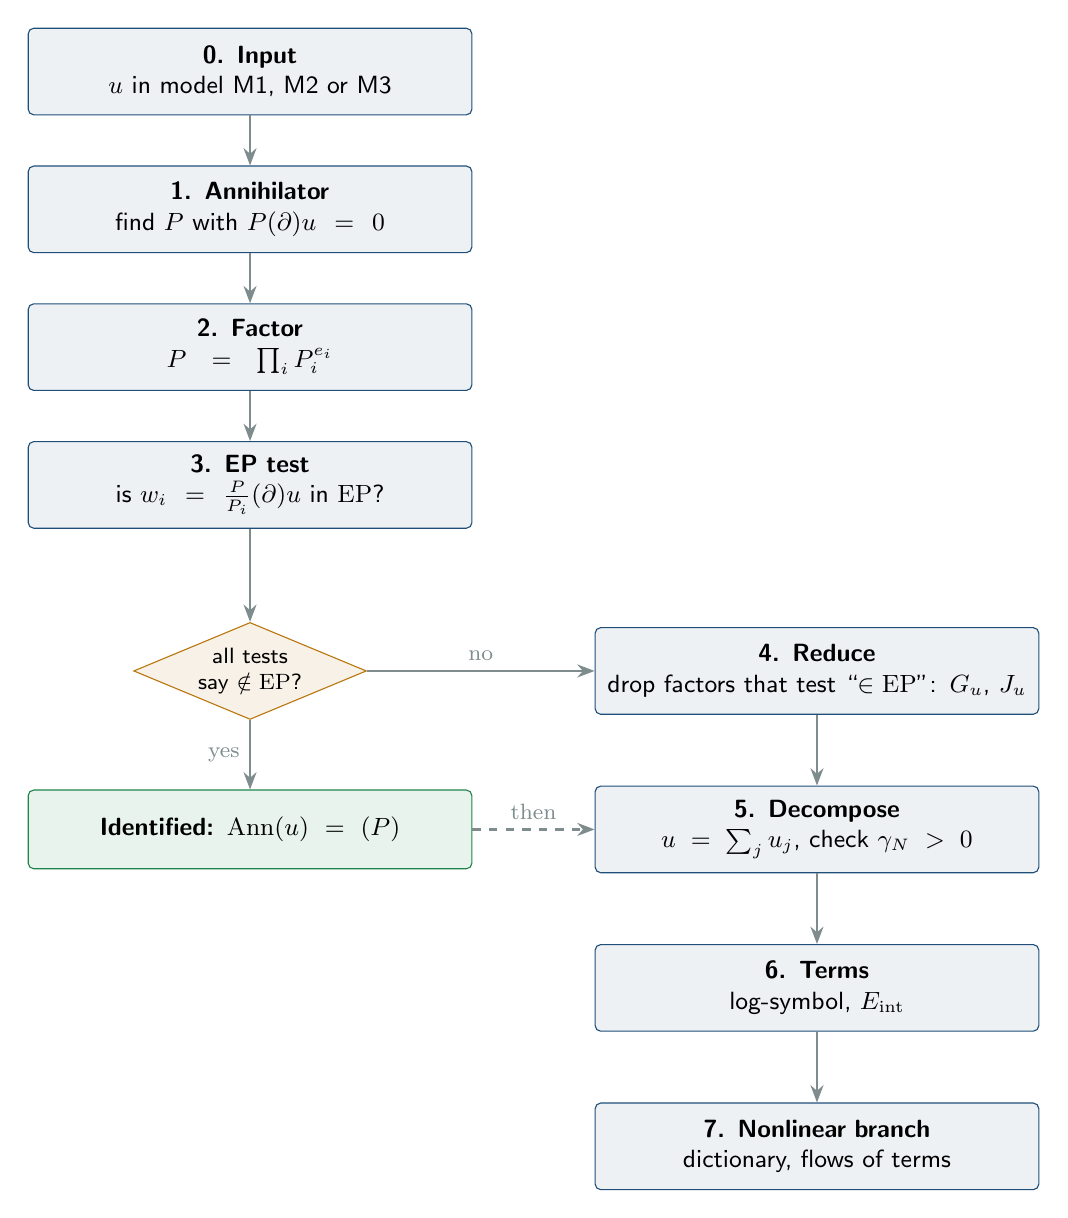
\begin{tikzpicture}[
  st/.style={draw=cA,fill=cA!8,rounded corners=2pt,minimum height=11mm,text width=5.4cm,align=center,font=\small\sffamily},
  dec/.style={draw=cD,fill=cD!10,diamond,aspect=2.4,inner sep=1pt,align=center,font=\footnotesize\sffamily},
  outb/.style={draw=cC,fill=cC!10,rounded corners=2pt,minimum height=10mm,text width=5.4cm,align=center,font=\small\sffamily},
  arr/.style={-{Stealth[length=2.2mm]},thick,cG}]
\def\dy{1.75}
\node[st] (s0) at (0,0) {\textbf{0. Input}\\ $u$ in model M1, M2 or M3};
\node[st] (s1) at (0,-\dy) {\textbf{1. Annihilator}\\ find $P$ with $P(\partial)u=0$};
\node[st] (s2) at (0,-2*\dy) {\textbf{2. Factor}\\ $P=\prod_iP_i^{e_i}$};
\node[st] (s3) at (0,-3*\dy) {\textbf{3. EP test}\\ is $w_i=\tfrac{P}{P_i}(\partial)u$ in $\EP$?};
\node[dec] (d) at (0,-4.35*\dy) {all tests\\ say $\notin\EP$?};
\node[outb] (o1) at (0,-5.5*\dy) {\textbf{Identified:} $\Ann(u)=(P)$};
\node[st] (s4) at (7.2,-4.35*\dy) {\textbf{4. Reduce}\\ drop factors that test ``$\in\EP$'': $G_u$, $J_u$};
\node[st] (s5) at (7.2,-5.5*\dy) {\textbf{5. Decompose}\\ $u=\sum_ju_j$, check $\gamma_N>0$};
\node[st] (s6) at (7.2,-6.65*\dy) {\textbf{6. Terms}\\ log-symbol, $\Eint$};
\node[st] (s7) at (7.2,-7.8*\dy) {\textbf{7. Nonlinear branch}\\ dictionary, flows of terms};
\draw[arr] (s0)--(s1); \draw[arr] (s1)--(s2); \draw[arr] (s2)--(s3); \draw[arr] (s3)--(d);
\draw[arr] (d)--node[left,font=\footnotesize]{yes}(o1);
\draw[arr] (d)--node[above,font=\footnotesize]{no}(s4);
\draw[arr] (s4)--(s5); \draw[arr] (s5)--(s6); \draw[arr] (s6)--(s7);
\draw[arr,dashed] (o1)--node[above,font=\footnotesize]{then}(s5);
\end{tikzpicture}
\caption{The algorithm as a flowchart. The left column certifies what the operator is. If every factor test says ``not an exponential-polynomial'', the operator is identified. Otherwise Step~4 reduces it to $G_u$. The right column extracts structure from $u$ once the operator is known.}\label{fig:algo}
\end{figure}

\subsection{The steps in detail}

\begin{aside}{Step 1: obtain an annihilator}
Let $\Phi(u)=(T_1u,\dots,T_Mu)^{\top}$ be the vector of $M$ candidate terms applied to $u$, and
\[
\mathbb G(u)=\int_\Omega\Phi\,\Phi^{*}\dd\mu
\]
its Gram matrix (positive semidefinite). A relation $\lambda\cdot\Phi=0$ holds if and only if $\lambda\in\ker\mathbb G(u)$. The computation is exact (rational or algebraic numbers, Gaussian elimination): no learning, no statistics. If $\ker\mathbb G$ has dimension larger than one, $u$ satisfies several relations, which is itself information about $G_u$ and $J_u$.
\end{aside}

\begin{aside}{Step 2: factor}
Factor $P(\tau,\xi)$ into irreducibles with multiplicities. This is a standard computer-algebra operation over the algebraic numbers.
\end{aside}

\begin{aside}{Step 3: exponential-polynomial test}
For each $i$ compute $w_i=(P/P_i)(\partial)u$ and decide whether $\dimc\ring w_i<\infty$. How depends on the data model:
\begin{itemize}
\item M1: a syntactic check (is the closed form a finite sum of polynomials times exponentials?);
\item M3: a holonomic computation, decidable modulo (AC) (Theorem~\ref{thm:holo});
\item M2: undecidable from the jet alone (Theorem~\ref{f:thm:blackbox}); with a bound $B$, compare annihilators up to degree $B+\deg P-1$ (Theorem~\ref{thm:decide}).
\end{itemize}
\end{aside}

\begin{aside}{Step 4: reduce to $G_u$}
Drop from $P$ each factor whose test returned ``EP'', with the multiplicity bookkeeping of Theorem~\ref{thm:intrinsic}: at most $\sum_ie_i$ tests in total. The output is $G_u$; the dropped part is $J_u$, whose finite zero set lists the exponentials contained in $u$. The certificate reads either ``$\Ann(u)=(P)$'' or ``$u$ identifies only $G_u$ and contains these exponentials''.
\end{aside}

\begin{aside}{Step 5: decompose}
For evolution factors $\tau-a_j(\xi)$ apply the Lagrange formula~\eqref{f:eq:lagrange}. For general coprime factors use the construction of Theorem~\ref{f:thm:factor}; the components are determined up to the $\delta(P)$-dimensional exponential-polynomial space, fixed by a normalisation. Before using the components in $H^m$, check $\gamma_N>0$ (Theorem~\ref{f:thm:hm}).
\end{aside}

\begin{aside}{Step 6: terms and interaction}
Inside an evolution factor with symbol $a=\sum_na_n$, the terms are read from the log-symbol, which is linear in time:
\[
\log\hat u(t,\kappa)=\log\hat u_0(\kappa)+t\sum_na_n(i\kappa).
\]
Then evaluate $\Eint$ by the product formula~\eqref{f:eq:eint} at cost $O(N)$ per mode. For non-commuting terms, classify the generated Lie algebra (Theorem~\ref{f:thm:lie}).
\end{aside}

\begin{aside}{Step 7: nonlinear case}
Replace Step~3 by the dictionary criterion (Theorem~\ref{f:thm:dict}) and Step~6 by the flow-based interaction term and its jet (Theorem~\ref{f:thm:jet}).
\end{aside}

\subsection{Worked example 1: the wave equation}

We follow Steps~1--5 on the wave equation with $c=1$ and the solution
\[
u(t,x)=\underbrace{\frac{1}{1+(x+t)^2}}_{f(x+t)}+\underbrace{e^{-(x-t)^2}}_{g(x-t)} .
\]

\begin{example}[{Step 1: annihilator}]
Take the dictionary $\{u_{tt},u_{xx},u_{tx},u_t,u_x,u\}$. The kernel of the Gram matrix is the line spanned by $u_{tt}-u_{xx}=0$. Output:
\[
P=\tau^2-\xi^2 .
\]
\end{example}

\begin{example}[{Step 2: factor}]
\[
P=Q_1Q_2,\qquad Q_1=\tau-\xi,\qquad Q_2=\tau+\xi .
\]
Two irreducible, simple factors.
\end{example}

\begin{example}[{Step 3: EP tests}]
\textbf{Remove $Q_1$.} We test $w_1=(\partial_t+\partial_x)u$. The two parts behave differently:
\[
(\partial_t+\partial_x)f(x+t)=2f'(x+t),\qquad (\partial_t+\partial_x)g(x-t)=0 .
\]
With $f(s)=1/(1+s^2)$:
\[
w_1=-\frac{4(x+t)}{\big(1+(x+t)^2\big)^2}.
\]
This is rational, not a finite sum of polynomials times exponentials: $w_1\notin\EP$.

\textbf{Remove $Q_2$.} Symmetrically, with $g(s)=e^{-s^2}$:
\[
w_2=(\partial_t-\partial_x)u=-2g'(x-t)=4(x-t)\,e^{-(x-t)^2}.
\]
A Gaussian times a polynomial is not an exponential-polynomial: $w_2\notin\EP$.
\end{example}

\begin{example}[{Step 4: reduce}]
Both tests say ``not EP'', so nothing is dropped. The point spectrum is empty, and the wave equation is identified:
\[
\Ann(u)=(\tau^2-\xi^2).
\]
\end{example}

\begin{example}[{Step 5: decompose}]
$(Q_1,Q_2)=(\tau,\xi)$, so $\delta(P)=1$. The components are $u_1=f(x+t)$ and $u_2=g(x-t)$, determined up to a constant moved from one to the other. Whether the components of every solution stay in $H^m$ on a given region is decided by Theorem~\ref{f:thm:hm}; on a square it holds (Example after Theorem~\ref{thm:density}).
\end{example}

\subsection{Worked example 2: advection--diffusion}

Now take the solution of Example~\ref{ex:advdiff},
\[
u=g(x-ct;\ \sigma^2+2Dt),\qquad c=2,\ D=\tfrac12,\ \sigma^2=1 .
\]

\begin{example}[{Steps 1--4}]
The Gram matrix of $\{u_t,u_x,u_{xx},u\}$ has kernel spanned by $u_t+2u_x-\tfrac12u_{xx}$, so
\[
P=\tau+2\xi-\tfrac12\xi^2 .
\]
It is irreducible (degree one in $\tau$). The test is on $u$ itself: a Gaussian is not an exponential-polynomial, so $\Ann(u)=(P)$ and the equation is identified.
\end{example}

\begin{example}[{Step 5}]
There is a single factor: no decomposition is needed.
\end{example}

\begin{example}[{Step 6: terms and interaction}]
The log-symbol is
\[
\log\hat u(t,\kappa)=\log\hat u_0(\kappa)+t\big(-2i\kappa-\tfrac12\kappa^2\big).
\]
Its two coefficients are the two terms: advection with speed $2$ and diffusion with constant $\tfrac12$. The interaction term follows from~\eqref{f:eq:eint}, at cost $O(2)$ per Fourier mode:
\[
\widehat{\Eint}(t,\kappa)=\big(e^{-2i\kappa t}-1\big)\big(e^{-\kappa^2t/2}-1\big)\,\hat u_0(\kappa).
\]
Figure~\ref{f:fig:eint} plots it.
\end{example}

\subsection{Cost and feasibility}

\begin{table}[!htb]
\centering\small
\begin{tabular}{@{}L{4.6cm}L{5.6cm}L{3.6cm}@{}}
\toprule
Component & Cost or feasibility & Source\\\midrule
annihilator from a dictionary & Gaussian elimination, $O(M^3)$ & Step 1\\
factorisation & standard computer algebra & Step 2\\
EP test, model M1 & syntactic & Step 3\\
EP test, model M3 & holonomic, decidable mod (AC) & Thm.~\ref{thm:holo}\\
EP test, black box & impossible without a bound & Thm.~\ref{f:thm:blackbox}\\
EP test with bound $B$ & linear algebra in degree $B+\deg P-1$ & Thm.~\ref{thm:decide}\\
components (evolution) & one rational multiplier per factor & Eq.~\eqref{f:eq:lagrange}\\
$\Eint$: value / by order / table & $O(N)$ / $O(N^2)$ / $\Theta(2^N)$ & Thm.~\ref{thm:cost}\\
\bottomrule
\end{tabular}
\caption{Cost and feasibility of the components of the algorithm.}\label{tab:complexity}
\end{table}

\begin{keypoint}
Every step of the algorithm is a theorem with explicit hypotheses. The algorithm is exact where the theorems are positive (Steps~2, 4, 5 and 6 on exponential-type data), and it reports honestly where they are negative (Step~3 on finite data, Step~6 in Sobolev spaces).
\end{keypoint}


% ---- end sections/full_ch10.tex


% ---- begin sections/full_ch11.tex
\section{Limits, open problems and status}\label{f:ch:status}
\sectionbrief
{no new assumptions.}
{to state what is impossible, what is open, which statements turned out false, and how reliable each result is.}
{delimits every claim of this edition.}

\subsection{What is impossible}

Each item below is a proved negative theorem, not a gap.
\begin{itemize}
\item a finite certificate of identification, and identification from a black box (Theorems~\ref{f:thm:nocert} and~\ref{f:thm:blackbox});
\item identification by restricting variable-coefficient operators to one solution (Proposition~\ref{prop:weyl});
\item decomposition of a solution by additive terms (Proposition~\ref{f:prop:terms});
\item factor decomposition on regions with holes, for some $P$ (Proposition~\ref{f:prop:holes});
\item components in $H^m$ in general: one derivative can be lost (Counterexample~\ref{f:cex:loss});
\item a continuous or stably regularised interaction term in $H^m$ (Theorems~\ref{f:thm:nocont} and~\ref{f:thm:noreg});
\item a finite product of single-term flows reproducing non-commuting dynamics when the adjoint orbit is infinite (Theorem~\ref{f:thm:lie}(c)).
\end{itemize}

\subsection{Statements that turned out false}

\begin{center}\small
\begin{tabular}{@{}L{5.2cm}L{6.0cm}L{2.6cm}@{}}
\toprule
Statement & Counterexample or correction & Ledger\\\midrule
the spectrum of an expansion decides identification on a bounded domain & $e^{x-t}$ on the unit square (Counterexample~\ref{cex:C3C1}) & C3-C1\\
components keep the regularity of $u$ & parallel transports on the square & C12-C1\\
$u\mapsto\Eint$ is continuous in $H^m$ & real exponentials in advection--diffusion & P1-P1(e)\\
the companion matrix is normal iff $p=s^m-c$ & $s^2+s-1$ & R6-T3\\
splitting by terms lies in $\ker(L_1,L_2)$ & $\tfrac12x^2+Dt$ for the heat equation & R2-T3 (corrected)\\
exact interaction impossible for infinite Lie algebras (as first stated) & $e^{-tT_2}e^{-tT_1}e^{t(T_1+T_2)}$ & R5-Q5, P1-C1\\
NLS identification by scattering data without multiplicity & explicit counterexample & OPF5D\\\bottomrule
\end{tabular}
\end{center}

\subsection{Open or conditional}

\begin{itemize}
\item closedness of the sum of kernels for $N\ge3$ differential factors \openq{} \led{C12-Q2}; solved for real transports in $L^2$;
\item density of the sum of kernels on non-convex regions \openq;
\item minimality of the bound $B$ on every region \openq{} \led{OP-ALG-Q2};
\item identification for analytic KdV data with nonzero reflection \openq{} \led{INT-Q1};
\item the uniform shock rate with several shock births \condl{} \led{OPA-Q1};
\item the exact values of the syzygy degrees $\delta_N(K)$ for general $N$ \openq{} \led{OPF5C-Q1};
\item no finite product of flows for $\partial_x^2$ and $x^k$, $k\ge3$ (the hypothesis of Theorem~\ref{f:thm:lie}(c) fails there) \openq{} \led{P1-Q3}, and Theorem~\ref{f:thm:lie}(c) without the assumption that the flows of $Y$ vanish at zero coupling \openq{} \led{P1-Q7}.
\end{itemize}

\subsection{How reliable the results are}

\textbf{Proofs and audits.} Every statement labelled \proved{} has a complete proof that passed an independent review. The reviewers were AI agents with no access to the author's reasoning, not human referees. Statements labelled \pw{} have complete proofs that were not audited; none of them is on the critical path of the main theorems.

\textbf{Formal verification.} Fifteen theorems of the algebraic core are formalised in Lean~4 with Mathlib, without \texttt{sorry}: the interaction identity for commuting flows, the comaximal factor decomposition with explicit projector, the normality criterion for $m=2$, and several irreducibility results. The analytic parts (distributions, Sobolev spaces, semigroups) are not formalised, because the libraries are missing.

\textbf{Citations.} Many ingredients are classical: Malgrange--Ehrenpreis, the Nullstellensatz, Cole--Hopf, inverse scattering. The primary sources of the load-bearing citations (Malgrange, Fulton, Kru\v zkov, Novikov) were checked; several others only on secondary sources. A result relied upon should be traced to its primary source.

\textbf{Novelty.} The contribution is the package: sharp characterisations, negative theorems and counterexamples, each with a verified status. Parts of the identification theory are folklore in commutative algebra (Oberst duality); parts of the finite-data theory are known in substance (Prony, Mourrain).

\subsection{What this edition does not contain}

\begin{itemize}
\item Phases~6--11: systems and matrix coefficients, variable coefficients and the analytic encoder, the universal dictionary, convergence, the extended algorithm. They are summarised in \emph{Punto di partenza} and will enter the complete edition after Phase~11.
\item The catalogue of about $60$ equation types and the tropical reading of scaling limits.
\item The Lean sources.
\end{itemize}


% ---- end sections/full_ch11.tex


% ---- begin sections/full_ch12_p05.tex
\section{Open problems and directions for improvement (Phases 0--5)}\label{ch:openimprove}
\sectionbrief
{the final report of Phases~0--5 (26 October 2026), the registry of open items, the route registry (Gates 1 and 4a) and the note on a learning pipeline.}
{Section~\ref{ch:status} states in a few lines what is open. This chapter gives the full list for Phases~0--5, what is already proved about each item, the improvements that would strengthen the work, the routes that were scouted and not taken, and the limits of the project.}
{a complete record. Items that were later closed, reduced or refuted in Phase~10 are marked; for those, the complete edition (Phases~0--10) prevails.}

\subsection{Still open or conditional at the end of Phase 5}

\begin{center}\small
\begin{longtable}{@{}L{2.6cm}L{3.6cm}L{5.2cm}L{3.0cm}@{}}
\toprule
Item & Question & Status and obstruction & Later\\\midrule\endhead
INT-Q1 (analytic data) & KdV, $r\not\equiv0$, $u$ analytic: is there an autonomous ODE in $x$? & open. New partial result OPF5C-T6: relations with non-singular origin force exponential tails; order $\le3$ gives $0$ or a $1$-soliton (with decay on the whole jet). Residual obstruction: singular relations at the origin, exactly where the cubic relation of Airy sits & reduced to (R) in Phase~10\\
OPA-Q1 general & several shock births & conditional on the localisation lemma L-loc (statement written in the audit S-CHECK-20) & closed modulo [F1]\\
OPA-Q2 density & density of the class Morse$+$(SB) & a sketch (Sard with finitely many parameters) & density proved\\
OPR2-Q2$'$ & wedges with degenerate directions & partial: the tangent model is closed and direct (OPF5B-P8); localisation to the polygon is missing & still open\\
OPR2-Q3 & repeated socle, ``no finite test'' & partial: proved under (I) existence of an identifying solution and (II) & characterised in Phase~10\\
OPF5C-Q1 & $\delta_N(K)$ for general $N$ and $N<K<2N-2$ & open; conjectures $\delta_N(2N-1)=N+2$, $\delta_N(2N-2)=N+4$, $\delta_N(2N)=N+1$ & computer-assisted cases added\\
S4ID-P8, OPR2-P7 & asymptotics with derivatives & conditional on [GT-u] (uniformity in $x$ is not stated by Grunert--Teschl; track: Deift--Zhou 1994) and on [Hm] & [Hm] proved\\
INT-T1(B) & reflectionless Hirota $N$-solitons & conditional on [F4$^-$] (the primary source in this form was not found; verified for $N=2$) & proved\\
non-convex regions & density of OPF5B-T1 outside convex sets & open & false for regions with holes\\
\bottomrule
\end{longtable}
\end{center}

\paragraph{Other open questions recorded in the text.}
\begin{itemize}
\item the closedness of the sum of kernels for $N\ge3$ differential factors \openq{} \led{C12-Q2} (solved for real transports in $L^2$);
\item minimality of the bound $B$ on every region \openq{} \led{OP-ALG-Q2};
\item no finite product of flows for $\partial_x^2$ and $x^k$, $k\ge3$ \openq{} \led{P1-Q3}, and Theorem~\ref{thm:lie}(c) without the assumption that the flows of $Y$ vanish at zero coupling \openq{} \led{P1-Q7};
\item P1-Q6: no continuity of the interaction term for any operator with two non-proportional terms \openq{} (\emph{false as written}, corrected in Phase~10).
\end{itemize}

\paragraph{Dependences that are modulo a source.} [F1] Lax--Oleinik $=$ Kru\v zkov (the source was read; an autonomous proof is missing); [L-loc]; [GT-u]; [F4$^-$]; and Malgrange 1966 for C3-P1 with general data on convex sets (the jet case is proved without it).

\subsection{Improving what is there}

\begin{itemize}
\item \textbf{Citations whose numbers were not checked}: Krantz--Parks Thm~2.3.5 (OP-T1), Cohen GTM 138 for (AC), H\"ormander SCV 1.4.4, Runge in Rudin. Of $112$ sources, $34$ had the theorem number checked and $75$ the content ($45$ only in the metadata); three wrong citations were corrected (Humphreys Cor.~B, Gel'fand--Dikii 1976, DLMF 9.7.10).
\item \textbf{Audits}: several statements are \pw{} (not audited); TROP-5--8 are written but not audited; the Gaussian example of Section~\ref{ch:interaction} and the Lagrange projector formula were derived for this edition and not literally in the ledger.
\item \textbf{Algorithm}: the Gram-matrix procedure of Step~1 is one way to obtain a candidate annihilator and has to be confirmed as the intended one; a cost analysis of each step is only indicative; the nonlinear branch has no full worked example.
\item \textbf{Fisher--KPP} is announced as a benchmark but only an estimate non-uniform in $t$ is recorded (S4T-P5); a statement or a removal is needed.
\item \textbf{Examples} suggested but not added: a worked example of the exact sequence of the dictionary criterion, and an example of a non-empty point spectrum with several factors.
\end{itemize}

\subsection{Routes scouted and not taken (Phases 1--5)}

Each candidate route was promoted, merged, parked or eliminated with a stated reason.
\begin{itemize}
\item \textbf{Promoted}: factor decomposition with the least common left multiple for variable coefficients (RT-1/R2b); the additive log-symbol for first-order evolutions (RT-2); the Wei--Norman and Dyson interaction analysis (RT-3); $\ker\mathbb G=\Ann(u)\cap\mathrm{span}$ and Prony $\Leftrightarrow$ Waring (RT-4); complete invariants (RT-6); the weighted Fock orthogonal basis (RT-R3a; extension to Airy open).
\item \textbf{Parked}: the symbol-tensor route RT-5 (the tensor keeps only the principal symbol; kept as a geometric invariant); RT-S1e, RT-S1f (no constant-coefficient theorem; only sectorial components); RT-R1b (needs a sign hypothesis on the datum); Koopman operators (``dynamic mode decomposition is regression''; to reopen with the normal form: eigenfunctions carry the nonlinear term); Painlev\'e, NLSPEC, HAANTJES (triggers in the nonlinear verdicts).
\item \textbf{Eliminated}: RT-S1g for the core (it gives no information for elliptic or parabolic operators), kept for the hyperbolic part.
\item \textbf{Scouted in Phases 3--4}: the tropical estimate of $E_{\rm int}$ from the symbol alone holds only on dissipative faces (TROP-3$'$, TROP-8); on conservative faces (Klein--Gordon, transport) no uniform estimate exists (TROP-4).
\end{itemize}

\subsection{The statistical wrapper that was proposed}

A learning pipeline was drafted around the exact analytic core and \emph{excluded} from the project by decision of the user (no machine learning). It is recorded as a direction: (1) an interpolation step returns a weighted family of smooth functions $(\hat u_s,\pi_s)$; (2) each is passed to the exact algorithm, which returns its factors and components; (3) the weights give a distribution over factors (``transport $0.7\pm0.1$, diffusion $0.3\pm0.1$''); (4) the distribution sets the parameters of a clustering, so that each group contains one factor; (5) repeat inside each group, with two measures of ``tangle'': the Friedrichs cosine between factors and $E_{\rm int}$ between terms. The exact parts exist; the interpolation, aggregation and clustering are a proposal, and the note asked whether the basis functions of the first step must be chosen in advance.

\subsection{What this edition does not contain}

The catalogue of about $60$ equation types and the tropical reading of scaling limits; the Lean sources; a human review (the reviewers were AI agents); Phases~6--10, which are in the complete edition.


% ---- end sections/full_ch12_p05.tex


\section*{Part II: beyond constant coefficients (Phases 6--10)}
\addcontentsline{toc}{section}{Part II: beyond constant coefficients (Phases 6--10)}
\noindent Sections~\ref{ch:systems}--\ref{ch:extalgo} extend the theory of Sections~\ref{sec:theory}--\ref{sec:nonlin} (Phases~0--5) to systems, variable coefficients, noisy and
finite data, encoders, dictionaries and the extended algorithm (Phases~6--10; Phase~11 was the audit of the whole). Each result names its proof as ``Dim.~An'' or ``Dim.~Bn'' in the
companion \emph{Catalogue of proofs} (directory \texttt{paper/analytical\_complete}).

% ---- begin sections/part2_ch12.tex
\section{Systems of equations and gauge}\label{ch:systems}
\sectionbrief
{a vector field $u=(u_1,\dots,u_k)$ on a connected open set $\Omega\subset\R^n$ that solves a system $P(\partial)u=0$ with a \emph{matrix} of constant coefficients $P\in R^{l\times k}$, $R=\C[\zeta_1,\dots,\zeta_n]$. The operator $P$ is not given.}
{the equations of physics that are not scalar (Dirac, Maxwell, elasticity) are systems; Phases~1--5 treated one scalar equation. We ask the same three questions: can one solution determine the system, when can a sum of kernels be split, and what does a change of gauge do to what can be known?}
{extends Sections~\ref{ch:ident}--\ref{ch:decomp} from $R$ to matrices over $R$. It supplies Step~3b of the extended algorithm (Section~\ref{ch:extalgo}). The proofs are Dim.~A32--A35 and B73--B78.}

\subsection{From one equation to a module}

For a scalar equation the annihilator $\Ann(u)$ was an ideal of $R$. For a system the object that replaces it is a \emph{module}. The rows of $P$ generate a submodule $U_P\subseteq R^{1\times k}$, and the quotient
\[
M_P=R^{1\times k}/U_P
\]
is the module of the system: solutions of $P$ are exactly the homomorphisms $M_P\to\mathcal A$ (Malgrange--Oberst duality). A vector $u$ \emph{identifies} $P$ when its annihilator $\Ann(u)=\{r:r(\partial)u=0\}$ equals $U_P$, i.e.\ when the map $M_P\to\mathcal A$, $[r]\mapsto r(\partial)u$, is injective.

\begin{intuition}
Think of $M_P$ as the list of everything the system says, up to consequences. A single function $u$ must carry all of it in an injective way. The obstruction is local: at a point $\lambda$ the solutions of the system that are pure exponentials $e^{\lambda\cdot x}$ form one line, but $M_P$ may contain a plane of ``independent'' behaviours at that point. A plane cannot be embedded in a line.
\end{intuition}

\subsection{When does an identifying solution exist?}

Define the \emph{socle} of $M$ at a maximal ideal $\mathfrak m_\lambda$ as the set of elements of $M$ killed by $\mathfrak m_\lambda$; it is the space of exponential behaviours $e^{\lambda\cdot x}$ the module contains.

\begin{theorem}[{Existence of an identifying solution \led{SYS-EX} \proved}]\label{thm:sysex}
Let $\Omega\subseteq\R^n$ be non-empty, open and connected. A finitely generated module $M$ embeds in $C^\infty(\Omega)$ (or $\mathcal D'(\Omega)$) if and only if $\dim_\C\mathrm{soc}_{\mathfrak m}(M)\le1$ for every maximal ideal $\mathfrak m$. In particular a system $P$ has an identifying solution if and only if $\dim\mathrm{Hom}_R(R/\mathfrak m,M_P)\le1$ for every maximal $\mathfrak m$.
\dimref{SYS-EX}
\end{theorem}

\begin{example}{Two ODE systems}
For $n=1$ let $P=\mathrm{diag}(s-1,s-1)$ (two copies of $u'=u$). The socle at $s=1$ has dimension $2$: no function $u$ ever identifies it. For $P=\begin{pmatrix}s-1&1\\0&s-2\end{pmatrix}$ all socles have dimension $\le1$, and $u=(ae^x-be^{2x},\,be^{2x})$ with $ab\ne0$ identifies it. In general an ODE system of rank $r$ with invariant factors $e_1\mid\dots\mid e_r$ has an identifying solution iff $e_1=\dots=e_{r-1}=1$ \led{SYS-T0} (known).
\end{example}

\begin{theorem}[{Square non-singular systems in two or more variables \led{SYS-C1} \proved}]\label{thm:sysc1}
If $n\ge2$ and $P\in R^{k\times k}$ has $\det P\ne0$, every socle of $M_P$ is zero, so on every connected $\Omega$ some $u\in\mathrm{Sol}(P)$ identifies $P$. The associated primes of $M_P$ are the prime factors of $\det P$.
\dimref{SYS-C1}
\end{theorem}

Dirac in $3+1$ dimensions, the matrix Klein--Gordon operator and the Lam\'e system of elasticity are all of this type. They always have an identifying field.

\begin{caution}[title=Where this is not new]
For $\Omega=\R^n$ the existence criterion is known (Oberst, Pommaret, Macaulay: the number of trajectories needed to generate a system). The new point here is only that $\Omega$ may be any connected open set, including one where $C^\infty(\Omega)$ is not an injective module.
\end{caution}

\subsection{Sums of kernels for systems}

For a scalar $P=Q_1Q_2$ we proved $\ker P=\ker Q_1+\ker Q_2$ on a simply connected region (Theorem~\ref{thm:factor}). For systems the analogue is stated with the \emph{least common left multiple}: if $U_1,U_2$ are the row modules of two sub-systems and $N=R^{1\times k}/(U_1+U_2)$, then $\mathrm{Sol}(Q_1)+\mathrm{Sol}(Q_2)=\mathrm{Sol}(P)$ requires $U_1\cap U_2=U_P$.

\begin{theorem}[{Sum of kernels \led{SYS-S1} \proved}]\label{thm:syss1}
On every open $\Omega$, $\mathrm{Sol}(Q_1)+\mathrm{Sol}(Q_2)=\mathrm{Sol}(P)$ implies $U_1\cap U_2=U_P$. Conversely, if $U_1\cap U_2=U_P$ and $\mathrm{Ext}^1(N,\mathcal A)=0$ the equality holds; this is the case when $\Omega$ is convex, and when $N$ has finite length and $H^1_{dR}(\Omega)=0$. The intersection $\mathrm{Sol}(Q_1)\cap\mathrm{Sol}(Q_2)$ is finite-dimensional iff $N$ has finite length, with dimension $\delta_{\rm sys}=\ell(N)$. For one scalar equation in two variables this is Theorem~\ref{thm:factor}.
\dimref{SYS-S1}
\end{theorem}

\begin{falsebox}{Simple connectivity does not suffice for infinite-length quotients}{\falsest}\label{cex:syss1}
There are a simply connected open $\Omega\subset\R^2$ (a ``U''-shaped domain) and $Q_1=(1,0)$, $Q_2=(1,\partial_x)$ with $U_1\cap U_2=U_P$ but $\mathrm{Sol}(Q_1)+\mathrm{Sol}(Q_2)\subsetneq\mathrm{Sol}(P)$, in $C^\infty$ and in $\mathcal D'$. The obstruction is the failure of $P$-convexity of $\Omega$, not its topology.
\dimref{SYS-S1}
\end{falsebox}

\subsection{Dirac in Hamiltonian form}

Write the free or perturbed Dirac equation as $L=I\partial_t+\sum_k\alpha^k\partial_k+B$ with arbitrary constant $4\times4$ matrices $\alpha^k,B$ (no Clifford relations are assumed).

\begin{theorem}[{Dirac coefficients are read exactly \led{H-DIRAC} \proved}]\label{thm:hdirac}
If $\psi\in\mathrm{Sol}(L_0)$ identifies $L_0$ and $L$ is another operator of this form with $L\psi=0$, then $L=L_0$: the matrices $\alpha^k$ and $B$ are determined by $\psi$ exactly, with no ambiguity. An identifying $\psi$ always exists. For massive Dirac in $3+1$ dimensions $M_D\cong(R/\mathfrak q)^{2}$ with $\mathfrak q=(p_0^2-|p|^2-m^2)$, and $\psi$ identifies $D$ iff $\psi_3,\psi_4$ are independent over $R/\mathfrak q$; in $1+1$ dimensions $\psi$ identifies $D_2$ iff $\psi_2\notin\EP$.
\dimref{H-DIRAC}
\end{theorem}

\begin{example}{Where the Dirac coefficients come from}
Normalising the coefficient of $\partial_t$ to the identity removes the ambiguity $D\sim VD$ of the covariant form $\gamma^\mu\partial_\mu$. In $1+1$ dimensions the identification test is just the one of Section~\ref{ch:ident}: the second component must not be an exponential-polynomial.
\end{example}

\subsection{Gauge, magnetic fields, and Lam\'e}

\begin{proposition}[{Gauge covariance and what invariant data reveal \led{G-L0, G-T2} \proved}]\label{prop:gauge}
Under $A\mapsto A+d\chi$, $u\mapsto e^{i\chi}u$ the covariant operators transform covariantly, so the identification tests are gauge-invariant. If the observation is invariant under the phase, a reconstruction of the potential $A$ recovers at most its gauge class $[A]$: $A'\sim A$ iff $dA'=dA$ and the holonomies agree (Aharonov--Bohm). On a simply connected region, $A'\sim A$ iff $dA'=dA$.
\dimref{G-T2}
\end{proposition}

\begin{proposition}[{Magnetic Schr\"odinger: one field does not identify $(A,V)$ \led{SYS-N3} \proved}]\label{prop:sysn3}
For $n\ge2$ and a nowhere-zero solution $u$ the pairs $(A',V')$ compatible with $u$ form an infinite-dimensional affine space, parametrised by divergence-free fields $k$; their magnetic fields differ, so they are not gauge-equivalent, even in the non-stationary case. The obstruction is a count: one complex scalar equation against $n+1$ real unknowns.
\dimref{SYS-N3}
\end{proposition}

\begin{proposition}[{Lam\'e in space \led{LAME-3} \proved}]\label{prop:lame3}
For $\rho,\mu\ne0$, $\lambda+\mu\ne0$, $\lambda+2\mu\ne0$, the system has $\det P=q_Pq_S^2$ with Bass multiplicities $1$ and $2$; an identifying displacement field exists, and $u$ identifies it iff $\mathrm{div}\,u$ satisfies no equation besides the wave equation of speed $\sqrt{(\lambda+2\mu)/\rho}$ and the two transverse polarisations of $\mathrm{rot}\,u$ satisfy no extra relation. A pure P-wave ($\mathrm{rot}\,u=0$) never identifies.
\dimref{LAME-3}
\end{proposition}

\begin{proposition}[{Dirac $1+1$ as an evolution: no uniform product \led{SYS-E1, E2, E3} \proved}]\label{prop:syse}
Writing $\psi_t=(X+mY)\psi$ with $X$ the transport and $Y$ the mass term, the operators $X,\mathrm{ad}_X^kY$ are linearly independent, so no finite product of transport and mass flows with $\xi$-independent times equals $e^{t(X+mY)}$ uniformly in the mass. The Lie algebra they generate is infinite-dimensional. An explicit product (Euler angles) exists, with times that are not polynomial in $\xi$ and with non-local Fourier multipliers.
\dimref{SYS-E}
\end{proposition}

\begin{proposition}[{Systems from finite data \led{SYS-R1} \proved}]\label{thm:sysr1}
From exponential-polynomial data one can identify only systems with finite-dimensional solution space; for an ODE system the identifying solution exists iff $e_1=\dots=e_{r-1}=1$.
\dimref{SYS-R1}
\end{proposition}

\begin{takeaway}
For a system the unknown is a module and the datum is one vector function. The only obstruction to identification is the socle, a purely algebraic and local count, and it vanishes for every non-singular square system in $n\ge2$ variables. What a single field can never do is separate gauge from physics.
\end{takeaway}

% ---- end sections/part2_ch12.tex


% ---- begin sections/part2_ch13.tex
\section{Variable coefficients}\label{ch:varcoef}
\sectionbrief
{a rectangle $\Omega=I\times J\subset\R^2$ and a solution $u$ of $iu_t=-u_{xx}+V\,u$, i.e.\ $L_0u=Vu$ with $L_0=i\partial_t+\partial_x^2$, where the potential $V(x)$ or $V(t,x)$ is unknown. Solutions are \emph{strong} (class SF): $u\in C^{1,2}(\Omega)$ and the equation holds almost everywhere.}
{in physics the coefficients are rarely constant: a Schr\"odinger particle feels a potential. Phases~1--5 identified constant coefficients. Here the unknown is a function, and the first question is whether a single solution can reveal it at all.}
{extends Section~\ref{ch:ident} from $\C$ to function coefficients. It supplies Step~3c of the extended algorithm (Section~\ref{ch:extalgo}). The proofs are Dim.~A36--A40 and B78.}

\subsection{Too much freedom: a huge class identifies nothing}

Suppose we allow coefficients in any algebra $\mathcal K$ of functions closed under differentiation (all smooth functions, all analytic functions). Then even one solution that never vanishes carries no information beyond itself.

\begin{theorem}[{Rank-one annihilator \led{VAR-N1, VAR-T1(a)} \proved}]\label{thm:varn1}
Let $u\in C^\infty(\Omega)$ have no zeros, with $a=u_t/u$ and $b=u_x/u$ in $\mathcal K$. Then the annihilator of $u$ among differential operators with coefficients in $\mathcal K$ is generated by $\partial_t-a$ and $\partial_x-b$, and the module $\mathcal K[\partial]u$ is isomorphic to $\mathcal K$ itself. For an affine family $L_\theta=L_0+\sum\theta_kT_k$ the compatible parameters are $\theta_0+\ker\Phi_u$, so $\theta$ is identified iff $\Phi_u(\theta)=\sum\theta_kT_ku$ is injective.
\dimref{VAR-N1}
\end{theorem}

\begin{intuition}
If the coefficient class is closed under differentiation, a zero-free $u$ can write each of its own derivatives as ``a coefficient times $u$'', so every law is a law about $u$ itself and nothing more. To identify anything the class of coefficients must be restricted in advance.
\end{intuition}

\begin{caution}[title=Zeros matter]
With zeros the statement fails: $u=t-x^2$ near $0$ satisfies no law $\partial_t+\alpha\partial_x+\beta$ with smooth coefficients, because at the origin it would give $1=0$.
\end{caution}

\subsection{A potential $V(x)$ is read from any non-zero solution}

For a time-independent potential the situation is the opposite: nothing can hide.

\begin{theorem}[{Identification of $V(x)$ \led{VAR-T1(b)} \proved}]\label{thm:vart1b}
Let $u\not\equiv0$ be a strong solution with potential $V\in L^\infty_{\rm loc}(J)$, and $X_0=\{x:u(t,x)=0\ \forall t\}$. Then $X_0$ is closed and discrete; if $L_0u=W(x)u$ for another $W$, then $W=V$ almost everywhere; and
\[
V(x)=\frac{iu_t+u_{xx}}{u}\qquad\text{at every }(t,x)\text{ with }u(t,x)\ne0 .
\]
\dimref{VAR-T1b}
\end{theorem}

\begin{intuition}
If $u$ vanished along infinitely many vertical lines accumulating at $x_0$, cutting $u$ off to the right of $x_0$ would give another strong solution that vanishes on a half-strip. Schr\"odinger waves have infinite speed, and a Carleman estimate (a weighted energy inequality) shows that a solution vanishing on a strip vanishes everywhere. So $u$ cannot have such lines, and the formula $V=(iu_t+u_{xx})/u$ holds on a set of full measure.
\end{intuition}

\begin{example}{The harmonic oscillator}
For $V=x^2$ and the Hermite functions $h_0,\dots,h_3$ the set $X_0$ is empty or $\{0\}$, and $(iu_t+u_{xx})/u$ returns $x^2$ exactly. The same formula recovers the P\"oschl--Teller and Airy potentials.
\end{example}

\subsection{A potential $V(t,x)$: silent strips}

\begin{theorem}[{Time-dependent potentials \led{VAR-T1(c)} \proved}]\label{thm:vart1c}
For $V\in C(\Omega)$, the potentials compatible with $u$ are $V+\{W:W=0\text{ on }\Omega\setminus Z(u)\}$, where $Z(u)=\{u=0\}$; so $V$ is identified iff $\mathrm{int}\,Z(u)=\emptyset$. If $\mathrm{int}\,Z(u)\ne\emptyset$ there is an open interval $T'\subset I$ with $u=0$ on $T'\times J$ (a \emph{silent strip}). Silent strips occur: Tychonoff's series gives a solution vanishing for $t\le0$ and non-zero for $t>0$. Hence ``every $u\not\equiv0$ identifies $V(t,x)$'' is false.
\dimref{VAR-T1c}
\end{theorem}

\begin{falsebox}{Data that switch on from the boundary}{\falsest}
On a bounded domain without boundary conditions, a solution can be identically zero up to a time and non-zero afterwards (Tychonoff's series). While it is silent every potential supported in the silent time is compatible with it. The failure is in the time direction: unique continuation holds in $x$ but not in $t$.
\end{falsebox}

\subsection{Stability and the phase}

\begin{theorem}[{Stability of the reconstruction \led{VAR-P3} \proved}]\label{thm:varp3}
On a rectangle $K$ with $|u_1|\ge\delta>0$: $\|V_1-V_2\|_\infty\le\delta^{-1}(1+\|V_2\|_\infty)\|u_1-u_2\|_{C^{1,2}(K)}$; the map is not continuous from $C^1$ to $L^\infty$ (an explicit oscillation); and under an a priori bound $M$ on $\|e_{tt}\|_\infty,\|e_{xxx}\|_\infty$ one has a H\"older modulus with sharp exponent $1/3$. It is a modulus of continuity, not a certificate.
\dimref{VAR-P3}
\end{theorem}

\begin{theorem}[{Unobserved phase: $V$ modulo constants \led{VAR-P4} \proved}]\label{thm:varp4}
If only the class $\{e^{i\theta(t)}u\}$ is observed, the compatible potentials are exactly $\{V+c:c\in\R\}$. For $P(\partial_t,L_q)u=0$ with $P$ unknown, $(P,q)$ is defined only modulo $q\to q+c$, $P(\tau,\ell)\to P(\tau,\ell-c)$: a redundancy of the parametrisation.
\dimref{VAR-P4}
\end{theorem}

\begin{proposition}[{Dirac $1+1$ with a potential \led{VAR-P5} \proved}]\label{prop:varp5}
Finite speed of propagation leaves regions that the data never visit: for $m=V=0$ a travelling bump $\psi=f(x-t)v_+$ vanishes for $x\le0.5$ and $x\ge1.7$, so every potential supported there is compatible. The matrix potential is determined at $x_0$ iff $\mathrm{span}_t\{\psi(t,x_0)\}=\C^2$.
\dimref{VAR-P5}
\end{proposition}

\subsection{Other results of this phase}

\begin{itemize}
\item \textbf{Algebra of differential operators with polynomial coefficients} (Weyl algebra): for a $D$-finite $u$ the annihilator is a principal left ideal and $u$ identifies iff its derivatives are independent over $K$; Airy is irreducible and every solution identifies; the oscillator is reducible exactly for $E\in\pm(2\N+1)$ \led{VAR-T2a, VAR-T6, VAR-E1, VAR-E2}.
\item \textbf{Dynamical Lie algebras}: $\dim\mathfrak g_V<\infty$ iff $V\in\mathrm{span}\{1,x,x^2\}$; the modified P\"oschl--Teller potential has an explicit evolution through a Darboux chain \led{VAR-P8}.
\item \textbf{Non-autonomous splitting}: $E^{\rm mult}=\iint[A_2(s_1),A_1(s_2)]+O(t^3)$; commuting at equal times is not enough \led{VAR-P9}. Dyson--Phillips converges for bounded time-dependent perturbations \led{VAR-P11}; Floquet logarithms are bounded but not differential \led{VAR-P12}.
\end{itemize}
These are list cards of the catalogue (Part~IV); the closures made in Phase~10 are in Section~\ref{ch:phase10}.

\begin{takeaway}
A function-valued coefficient is identified by one solution exactly when the solution cannot hide: for $V(x)$ it cannot (infinite speed and unique continuation); for $V(t,x)$ it can fall silent; for a huge class of coefficients, nothing is identified. Stability is of order two and the phase costs one constant.
\end{takeaway}

% ---- end sections/part2_ch13.tex


% ---- begin sections/part2_ch14.tex
\section{Convergence, noise and the limits of learning}\label{ch:convergence}
\sectionbrief
{one analytic function $u$ on a connected open set $\Omega\subset\R^n$, observed through its Taylor jet at a point $p_0$ (the datum at step $K$ is $j_Ku$), or through a noisy copy $\tilde u$ with $\|\tilde u-u\|\le\delta$ in a stated norm.}
{Sections~\ref{ch:ident} and~\ref{ch:data} proved that no finite amount of data certifies identification. A real experiment gives more and more data: does the identified operator converge, how fast, and what can a noisy measurement still say?}
{supplies Steps~1--4 and~7 of the extended algorithm (Section~\ref{ch:extalgo}). The proofs are Dim.~A41--A43.}

\subsection{Identification in the limit}

At step $K$ the rule computes, for each degree $m\le K$, the space $N_{m,K}$ of operators of degree $\le m$ whose action on $u$ has vanishing Taylor coefficients up to order $K-m$. These spaces decrease with $K$ and their limit is $\Ann(u)\cap R_{\le m}$. The \emph{minimal-degree rule} outputs the gcd of $N_{m^*(K),K}$ at the smallest degree $m^*(K)$ where it is non-zero.

\begin{theorem}[{Identification in the limit \led{CONV-L1, CONV-T1} \proved}]\label{thm:convt1}
If $\Ann(u)\ne0$ with minimal degree $d$, the rule outputs $g_d=\gcd(\Ann(u)\cap R_{\le d})$ from some step on; if $\Ann(u)=(P)$ it outputs $P$, without knowing $\deg P$; if $\Ann(u)=0$ the degree $m^*(K)\to\infty$. The sequence of outputs takes at most $(d+1)(d+2)/2$ values. But:
\begin{itemize}
\item the step $K^*$ after which the output is correct is not bounded by any function of $d$;
\item no function of the jet of order $K$ is a correct certificate: any finite jet is shared by a polynomial, whose annihilator is a different ideal.
\end{itemize}
\dimref{CONV-T1}
\end{theorem}

\begin{example}{Convergence at an unpredictable time}
For $u=1+x^{N+2}e^{x^2}$ one has $\Ann(u)=(\tau)$. The rule outputs ``no law of degree $1$'' for $K\le N+1$ and $\tau$ from $K=N+2$, for every $N$: nothing in the first $N+1$ derivatives announces the law.
\end{example}

\subsection{No learner decides whether a law exists}

\begin{theorem}[{Analytic Gold theorem \led{CONV-T2, CONV-T2$'$} \proved}]\label{thm:convt2}
For any sequence of maps $\varphi_K$ from jets of order $\le K$ to $\{\text{law},\text{no law}\}$ (no computability or measurability assumed) there is a real entire function $u$ on which $\varphi_K(j_Ku)$ does not converge to the correct answer. The same holds restricted to the class where $\Ann(u)$ is principal or zero; hence no learner identifies $\Ann(u)$ on that class.
\dimref{CONV-T2}
\end{theorem}

\begin{intuition}
Build $u$ as a limit of polynomials. Whenever the learner says ``law'' on the current polynomial (it must, eventually), add Taylor coefficients, chosen outside a proper algebraic set, that destroy every law of degree $\le k$. The limit function is differentially transcendental yet agrees with a polynomial where the learner said ``law'', infinitely often.
\end{intuition}

\begin{keypoint}
``$\Ann(u)\ne0$'' is \emph{verifiable in the limit} (a rule that is eventually right when it holds) but not \emph{decidable in the limit}.
\end{keypoint}

\subsection{Noisy data}

\begin{theorem}[{Noise: discontinuity, conditional stability, discrepancy rule \led{CONV-T3, T4, T5} \proved}]\label{thm:convt45}
(T3) In spaces where polynomials are dense and $e^{|z|^2}$ lies, the sets $\{\Ann=0\}$ and $\{\Ann\ne0\}$ are both dense: $u\mapsto\Ann(u)$ is discontinuous everywhere. (T4) At a fixed level $n_0$ with a margin $\rho=\sigma_2(\Phi(u))>0$, the minimal singular vector of $\Phi(\tilde u)$ is within $\sin\angle\le2\delta/\rho$ of the true law, an order that is optimal; under an $L^2$ error and an a priori $H^{n_0+s}$ bound the rate is H\"older, and $\sigma_1(\Phi(\tilde u))>\delta$ certifies a misfit. (T5) The discrepancy rule $m(\delta)=\min\{m:\sigma_1(\Phi_m(\tilde u))\le\delta_m\}$ returns the correct degree $d$ and converges at rate $\delta$ once $\delta<\delta_0=\tfrac12\min_{m<d}s_m$; if $\Ann(u)=0$, $m(\delta)\to\infty$. The threshold $\delta_0$ cannot be bounded below from the data.
\dimref{CONV-T4}
\end{theorem}

\begin{example}{The heat kernel from noisy data}
For $u=(t+1)^{-1/2}e^{-x^2/(4(t+1))}$ (minimal degree $2$, $\Ann=(\tau-\xi^2)$), the rule returned $m(\delta)=2$ for $\delta=10^{-3}$ and $10^{-4}$ in a numerical check.
\end{example}

\subsection{Other results of this phase}

\begin{itemize}
\item \textbf{Locality}: when the law is a non-local operator it is invisible to $\Ann(u)$; an irrational fractional power or a delay gives $\Ann=0$ (a delay is in the local class through an auxiliary transport) \led{CONV-T6, CONV-P6, CONV-P7}.
\item \textbf{Dimension $1+d$}: the ambiguity of the factor decomposition is infinite unless the factors are pairwise co-maximal \led{CONV-D1}; on a convex region $\ker(Q_1Q_2)=\ker Q_1+\ker Q_2$ in $C^\infty$ \led{CONV-D2}.
\item \textbf{Boundary conditions} are invisible to $\Ann(u)$; stability holds for a dictionary of traces \led{CONV-B1--B3}. Splitting with a Dirichlet boundary has global order $1$ (Lie) and $\Theta(h^{5/4})$ (Strang) in $L^2$ \led{CONV-T8}.
\item \textbf{Mori--Zwanzig} for constant-coefficient $2\times2$ systems: exact memory form and eliminated law \led{CONV-MZ1--3}; the criterion ``$E_{\rm int}=0\iff[\mathcal P,L]=0$'' is false \led{CONV-MZ3-F}.
\item \textbf{A convergence contract} for chains of steps: classes (A) exact, (B) convergent with explicit error, (C) no guarantee, (Lim) in the limit; the error of a chain of Lipschitz steps is $\le\sum_i(\prod_{j>i}L_j)\varepsilon_i$ \led{CONV-T7}.
\end{itemize}

\begin{takeaway}
Learning an operator from growing data is possible only in the limit and without a certificate; deciding whether any law exists is impossible even in the limit; and noise can be handled only relative to a finite level of the dictionary and a margin that the data cannot supply.
\end{takeaway}

% ---- end sections/part2_ch14.tex


% ---- begin sections/part2_ch15.tex
\section{The analytic encoder}\label{ch:encoder}
\sectionbrief
{a Schr\"odinger-type equation with a variable potential $q(x)$ \emph{known}, written $P(\partial_t,L_q)u=0$ with $L_q=-\partial_x^2+q$ and $L_0=-\partial_x^2$, on a symmetric interval $J$.}
{the variable potential is a nuisance: the theory of Phases~1--5 applies to $L_0$. Can one change the unknown by an explicit, invertible, stable map so that the potential disappears, without machine learning? Such a map is an \emph{encoder}.}
{supplies Step~5 of the extended algorithm (Section~\ref{ch:extalgo}): the encoder is a \emph{translation} to constant coefficients, not a source of information. The proofs are Dim.~A44--A47 and B79.}

\subsection{What an encoder is}

A \emph{structured encoder} is a linear map $W$ acting in $x$ only, with (E1) finite-dimensional kernel on its own domain, (E2$'$) $WL_q=(L_0+c)W$ for a constant $c$, and (E3) explicit. The conditions are all needed: without (E1) the zero map qualifies, and without (E3) the interaction-picture map $U_0(t)U_V(t)^{-1}$ does.

\begin{proposition}[{A constant potential has no strict differential intertwiner \led{ENC-K0} \proved}]\label{prop:enck0}
For $q\equiv c\ne0$ no differential operator of any order satisfies $WL_c=L_0W$. With the relaxed requirement $WL_c=(L_0+c)W$ the identity works.
\dimref{ENC-K0}
\end{proposition}

\subsection{The Volterra transformation operator}

Let $K$ solve the Goursat problem $K_{xx}-K_{ss}=q(x)K$ on the triangle $|s|\le|x|\le a$, with $K(x,x)=\tfrac12\int_0^xq$ and $K(x,-x)=0$, and put
\[
Tf(x)=f(x)+\int_{-x}^xK(x,s)f(s)\dd s,\qquad W=T^{-1}.
\]

\begin{theorem}[{The symmetric Volterra encoder \led{ENC-1, ENC-U1} \proved}]\label{thm:enc1}
For $q\in C^1$ the problem has a unique solution, and for every $f\in C^2(J)$, without any boundary condition, $L_qTf=TL_0f$ with $(Tf)(0)=f(0)$, $(Tf)'(0)=f'(0)$. $T$ is bijective on $C$, $C^2$ and (for $q\in C^\infty$) $C^\infty$, with $\|K\|\le\frac{aQ}2e^{a\sqrt Q}$ and a Lipschitz dependence on $q$. Among all Volterra intertwiners the one preserving Cauchy data at the base point is unique; it depends on the base point already for constant $q$.
\dimref{ENC-1}
\end{theorem}

\begin{intuition}
In characteristic coordinates the kernel solves a Volterra integral equation by successive approximations, with the bound $(Q|\xi\eta|/4)^n/(n!)^2$. Volterra operators with a triangular kernel have no spectrum, so $T$ is invertible, and the Goursat conditions are exactly the ones that make every boundary term in the Leibniz expansion of $L_qTf-TL_0f$ cancel.
\end{intuition}

\begin{corollary}{One encoder for every equation \led{ENC-C1} \proved}\label{cor:encc1}
For $q\in C^\infty$ and every polynomial $P$: $P(\partial_t,L_q)u=0\iff P(\partial_t,L_0)(Wu)=0$. The same $W$ serves Schr\"odinger, heat, wave and Klein--Gordon.
\dimref{ENC-C1}
\end{corollary}

\begin{example}{Constant potential}
For $q\equiv c$ the transformation maps the exponential $e^{ik\cdot}$ to $e^{ikx_0}[\cos\mu(x-x_0)+ik\sin\mu(x-x_0)/\mu]$ with $\mu^2=k^2-c$: the eigenfunction of $L_c$ with the Cauchy data of $e^{ikx}$ at $x_0$.
\end{example}

\subsection{What no encoder can do}

\begin{theorem}[{No time-independent encoder for a time-dependent potential \led{ENC-P0} \pw}]\label{thm:encp0}
Let $W$ be linear with finite kernel and $W(-\partial_x^2+V(t,\cdot))f=(-\partial_x^2+c(t))Wf$ for all $t$. Then $V(t,x)-V(s,x)=c(t)-c(s)$: the potential must be autonomous up to a function of time. The reason is that otherwise infinitely many independent functions $m\varphi_k$ would lie in $\ker W$. Encoders for a genuinely time-dependent potential exist but depend on time (interaction pictures), and a pointwise representative with the identity time change exists exactly for $V=\beta(t)x+\gamma(t)$.
\dimref{ENC-P0b}
\end{theorem}

\begin{theorem}[{Blind encoders and identifiability \led{ENC-N1$'$} \proved}]\label{lem:encn1}
A blind encoder, one whose output does not depend on which potential produced the data, exists iff the coherence condition (C) holds for the chosen family; it is implied by identifiability and is strictly weaker (a witness: the data model that observes only a phase). The correct statement is: blind encoder $\iff$ identifiability modulo the gauge group of the data model.
\dimref{ENC-N1p}
\end{theorem}

\begin{caution}[title=An earlier claim that turned out false]
The synthesis of the first version, ``the exceptions change the time'', was false as written: Avron--Herbst and the whole class $V=\beta(t)x+\gamma(t)$ have a pointwise representative with the identity time change. Likewise ``a blind encoder exists iff $W_V^{-1}v$ is injective'' is false (ENC-N1).
\end{caution}

\subsection{Other results of this phase}

\begin{itemize}
\item \textbf{Darboux encoders}: a differential $W$ with $WL_q=(L_0+c)W$ is a Darboux chain on each component of a complement of a countable closed set; for rational $V\to0$ it exists iff $V$ is an iterated Darboux transform of $0$ (Adler--Moser) \led{ENC-K1$'$, ENC-K1}. They are unbounded with a non-trivial kernel, so they lose modes.
\item \textbf{The interaction term with a potential}: $\|E^{\rm mult}f\|\le\frac{t^2}2(\|V''\|\|f\|+2\|V'\|\|f'\|)+\frac{2t^3}3\|V'\|^2\|f\|$ with the optimal constant $2/3$, and $E^{\rm mult}\equiv0$ iff $V$ is constant \led{ENC-A9}.
\item \textbf{Faddeev decomposition} on an interval and \textbf{Foldy--Wouthuysen} for the free Dirac $1+1$ are decompositions, not encoders \led{FAD-1, FW-1}.
\end{itemize}

\begin{takeaway}
Removing a variable potential is possible by an explicit stable Volterra transformation when the potential is known, and the same map works for every equation in $(\partial_t,L_q)$. When the potential is unknown the encoder gives no information, and for a time-dependent potential no time-independent encoder exists.
\end{takeaway}

% ---- end sections/part2_ch15.tex


% ---- begin sections/part2_ch16.tex
\section{The universal dictionary and the misfit certificate}\label{ch:dictionary}
\sectionbrief
{a filtered dictionary $\mathcal D_0\subset\mathcal D_1\subset\cdots$ of finite sets of operators (the \emph{atoms}), enumerated by an explicit algorithm; a datum $u$ \emph{fits} a level if some non-zero combination of its atoms annihilates $u$.}
{the project was asked: can a dictionary be built that ``takes everything into account''? The honest answer has three parts: in the sense of approximation, yes; as exact identification of every operator, no; and in between, a misfit can always be certified by finite data, while a fit never can.}
{supplies Steps~2 and~4 of the extended algorithm (Section~\ref{ch:extalgo}). The proofs are Dim.~A48--A51.}

\subsection{What ``universal'' can mean}

\begin{theorem}[{Every local linear operator is a limit of dictionary elements \led{DICT-U1} \proved}]\label{thm:dictu1}
By Peetre's theorem a linear operator on $C^\infty(\Omega)$ that does not enlarge supports is a differential operator with smooth coefficients, of locally finite order. With a partition of unity and polynomial approximation of the coefficients it is a limit, in the topology of locally bounded order, of elements of the explicit dictionary $\{\chi_j(y)y^\beta\partial^\alpha\}$. It is a pointwise limit of polynomial-coefficient operators iff its order is globally finite.
\dimref{DICT-U1}
\end{theorem}

The same holds for classes beyond differential operators: regular non-linear operators (differential polynomials, by a local version of a Peetre--Slov\'ak argument), symbols with loss $\varepsilon$, completely monotone memory kernels, delays (as an augmented transport system) and systems, each with its own explicit atoms \led{DICT-U2, U3, RIT1, U4}.

\subsection{What it cannot mean}

\begin{theorem}[{No countable dictionary identifies everything \led{DICT-N1} \proved}]\label{thm:dictn1}
(i) For any countable dictionary the exactly representable operators form a meagre set (Baire). (ii) No finite data certifies the fit or the identification. (iii) If $u\in\EP$, at every high level $\Ann(u)\cap R_{\le n}\supsetneq(L)\cap R_{\le n}$ for any single law $L$: the kernel is strictly larger than the consequences of one law. (iv) A procedure with finite outputs emits only countably many operators. (v) For a filtered family of differential polynomials the set of $u$ that satisfy some equation of the dictionary is meagre \emph{and} shy (prevalence): the generic $u$ satisfies none.
\dimref{DICT-N1}
\end{theorem}

\begin{intuition}
A compact set in an infinite-dimensional space has empty interior, so a countable family of finite-parameter families covers a ``thin'' set. For the measure statement one moves $u$ along a direction on which the determinant of the dictionary applied to $u+sw$ is a non-zero polynomial in the single real parameter $s$: only finitely many $s$ lie in the bad set.
\end{intuition}

\begin{caution}[title=What this theorem does not say]
``Everything'' holds in the sense of approximation (Theorem~\ref{thm:dictu1}) plus a misfit certificate, not as exact identification. The first form of the statement for coefficients that are $C^\infty$ functions (``no operator is identified'') is false and was replaced by a rank theorem: an affine family is identified iff $\ker\Phi_u=0$ \led{DICT-RANGO}.
\end{caution}

\subsection{Fit and misfit}

\begin{theorem}[{Asymmetry of fit and misfit \led{DICT-A, MF1--MF3} \proved}]\label{thm:dicta}
Let $\{D_0,\dots,D_N\}$ be independent continuous operators. The set of $u$ with a \emph{misfit} (the $D_iu$ independent) is open, and each such $u$ has a certificate: a non-vanishing determinant $\det\langle D_iu,\psi_j\rangle$ for finitely many test functions, valid in a neighbourhood. The set of $u$ that \emph{fit} is closed with empty interior, and for differential atoms a fit cannot be certified even from finitely many \emph{exact} measurements.
\dimref{DICT-A}
\end{theorem}

\begin{example}{A certified misfit, an uncertifiable fit}
For $u=e^{-t}\sin x$ the level $\{\partial_t,\partial_x\}$ shows a misfit: the Gram matrix of $(u_t,u_x)$ is non-singular and $\varphi=\langle\cdot,\mathrm{res}\rangle/\|\mathrm{res}\|$ certifies that no first-order law holds. The level $\{\partial_t,\partial_x^2\}$ fits ($u_t=u_{xx}=-u$), and no finite data can certify that.
\end{example}

Misfit certificates exist in three forms: a Hahn--Banach functional (distance to the span), a Gram quotient in a Hilbert space, and a weak form that needs no derivative of $u$ (only integrals against test functions) \led{MF1, MF2, MF3}.

\subsection{Stopping rules and the limit}

\begin{theorem}[{Stopping rule and identification in the limit \led{DICT-GR, I-LIM} \proved}]\label{thm:dictgr}
If $n_0$ is the least level with an affine fit and the kernel at every higher level equals the consequences of that law, then the test stops exactly at $n_0$. With a compact class of coefficients and uniqueness, small residual means close coefficients: $\|L_n-L\|\le\omega(C_u\varepsilon_n)$, and with data of error $\delta$ one gets $\omega(C_u\varepsilon_n+2C_{R'}\delta)$, a H\"older rate in the one-coefficient case.
\dimref{DICT-GR}
\end{theorem}

\subsection{Other results of this phase}

\begin{itemize}
\item \textbf{Exact gain of an atom} \led{DICT-R3}; \textbf{change of frame} by the Volterra encoder, with exact intertwining and constants $\|W\|,\|W^{-1}\|\le1+a^2Q\,e^{a\sqrt Q}$ \led{DICT-R6}.
\item \textbf{Exponential families}: exact polynomialisation, kinks and the $2$-kink \led{DICT-NS}.
\item \textbf{Minimax rate} $\Theta(\varepsilon^{1/3})$ for the potential reconstruction under $M>\delta_0$ \led{DM-$\delta$-MINIMAX}.
\end{itemize}

\begin{takeaway}
A dictionary can be universal for approximation, never for exact identification. Its negative side is both topological and measure-theoretic; its positive side is a one-way certificate: misfit is witnessed by finitely many integrals, fit by none.
\end{takeaway}

% ---- end sections/part2_ch16.tex


% ---- begin sections/part2_ch17.tex
\section{What Phase 10 changed}\label{ch:phase10}
\sectionbrief
{the open problems and conditional statements of all earlier phases, reviewed in Phase~10 by three research sessions (phases 1--4, phase 5, phase 8), each followed by an independent audit and, where needed, a second round.}
{an honest edition has to say which earlier statements were refuted, which were closed, and which remain open. Phase~10 refuted five of them and closed many.}
{in case of a difference with Sections~\ref{ch:interaction}, \ref{ch:regular} and \ref{ch:nonlin} this section prevails. The proofs of the two corrections that change statements are Dim.~A52 and A53; the other items are list cards (Part~IV).}

\subsection{Statements that turned out false}

\begin{proposition}[{The interaction no-go with constant terms \led{S10A-T1, P1-Q6} \proved}]\label{thm:s10at1}
Section~\ref{ch:interaction} left open (P1-Q6) whether $u_0\mapsto E_{\rm int}$ fails to be continuous in $H^m$ for every operator with at least two non-proportional terms. The statement as written is \textbf{false}: for reaction--diffusion $u_t=Du_{xx}+ru$ (two non-proportional terms) $E_{\rm int}$ is continuous from $H^1$, with
\[
E_{\rm int}(u)=(e^{sr}-1)\big(v(t)-v_0\big),\qquad s=t-t_0 .
\]
The correct form is: for monomial terms of distinct degrees, $E_{\rm int}$ is unbounded $H^m\to L^2$ for every $m$ and base time iff there are \emph{at least two terms of degree $\ge1$}; with at most one the interaction is bounded for every $m\ge1$. Constant terms only multiply the solution by a bounded exponential and neither create nor destroy the no-go.
\dimref{S10A-T1}
\end{proposition}

\begin{proposition}[{Holes: the sum of kernels is closed but not dense \led{S10A-P1} \proved}]\label{prop:s10ap1}
On the annulus $A=\{1<|z|<2\}$ the Laplacian is a product of the two coprime factors $\partial_t\pm i\partial_x$. The harmonic function $\log|z|$ is not in the closure of the sum of holomorphic and anti-holomorphic functions in any $H^m$, and for $m\ge1$
\[
\ker_{H^m(A)}\Delta=(\mathcal H_1+\mathcal H_2)\oplus\C\log|z| :
\]
the sum is closed, of codimension $b_1=1$, and not dense. Hence the density question of Section~\ref{ch:regular} has a negative answer on non-convex regions in general (P2-Q1 is false as a universal statement), and this is a \emph{differential} example of ``closed but not dense''.
\dimref{S10A-P1}
\end{proposition}

\begin{intuition}
A hole gives a period: the flux of a harmonic function through a loop around the hole. The flux is a continuous functional that vanishes on holomorphic and anti-holomorphic pieces (their derivative has a single-valued primitive), but not on $\log|z|$.
\end{intuition}

Three more statements were refuted: the extension of the convex density theorem to non-convex regions (S10B-C1, by a hole with an interior); P2-Q1 as a universal statement (for $\Delta$ on every Lipschitz region with $b_1\ge1$); and, in the variable-coefficient phase, ``$P11(e)$ with $B$ merely continuous'' and ``the pole depends only on $A(\xi_0)$ and the factorisation''.

\subsection{Problems closed}

\begin{itemize}
\item \textbf{Density of the sum of kernels} on every simply connected Lipschitz region, and for $\delta(P)=0$ on every Lipschitz region, modulo two cited facts [F1], [F2]; the source of the collar field was replaced by a proof \led{S10A-T3, S10COL}.
\item \textbf{C12-P7}: ``closed but not dense'' realised by the annulus.
\item \textbf{C3-Q1}, the decidability question, closed as a \emph{classification by data model} (composition of black-box impossibility, bound, analytic and jet models); no new mathematics.
\item \textbf{OPF5C-T5, INT-T1(B), S10B-T2}: the multi-soliton is a Hirota solution; the reflectionless Jost computation holds.
\item \textbf{Uniform shock rate with several births} (OPA-Q1): modulo the equivalence Oleinik $\Leftrightarrow$ Kru\v zkov [F1].
\item \textbf{Variable coefficients}: VAR-P11(e) by Volterra and Gronwall; a solution with $V=0$, $|Z|>0$ and $\mathrm{int}\,Z=\emptyset$ (Tychonoff and a Cantor-type set); Floquet in the quadratic class ($\mathrm{tr}M=-26/5$); a monic criterion in the Weyl algebra.
\item \textbf{Systems}: Maxwell has an identifying field; at fixed real time no finite product of Dirac flows with polynomial times; the pole criterion $E_0\cap F_0\ne0$.
\item \textbf{Dictionary}: the $L^1$ rate for general completely monotone memory kernels; the minimax rate $\Theta(\varepsilon^{1/3})$.
\item \textbf{Computer-assisted}: $N\le4$, and, after the triage, $N=5$ and $\delta_6(12)=7$ for the syzygy degrees (modulo a novelty hypothesis (Nov)); $\delta_6(11)=8$ with a written proof.
\end{itemize}

\subsection{Textbook examples and formalisation}

Five textbook examples were checked against the whole theory: free Dirac $1+1$, the harmonic oscillator, the P\"oschl--Teller potential, the fractional heat equation and Maxwell in vacuum; $80$ of $80$ checks pass, and three new arguments were proved. The formalisation in Lean~4 with Mathlib reached $37$ entries: $27$ are faithful to the ledger statement, $7$ are weaker and $3$ are different, none is vacuous, and all $85$ \texttt{\#print axioms} use only the standard axioms. Mathlib has no Weyl algebra and no $C_0$-semigroups, so the analytic parts are not formalised.

\begin{takeaway}
The corrections of Phase~10 all push in one direction: the negative results of Phases~1--3 are sharper than first stated (constants do not break the no-go; holes do break density), and the closures are explicit about what they depend on.
\end{takeaway}

% ---- end sections/part2_ch17.tex


% ---- begin sections/part2_ch18.tex
\section{The extended algorithm}\label{ch:extalgo}
\sectionbrief
{the results of Sections~\ref{ch:systems}--\ref{ch:dictionary} and of the algorithm of the companion paper; a datum in one of the models below.}
{the algorithm of the companion paper turned the theorems of Phases~1--5 into a seven-step procedure for a scalar constant-coefficient equation. This section extends it to systems, variable coefficients, noise, and operators outside the catalogue, and states, for every step, what is promised and what is not.}
{the operational summary of the whole edition. It introduces \emph{no new claim}: it composes rows of the ledger.}

\subsection{Which senses of ``identify''}

The word ``identify'' has five senses, and every step declares which one it uses.

\begin{center}\small
\begin{tabular}{@{}L{1.7cm}L{7.3cm}L{5.4cm}@{}}
\toprule
Sense & Meaning & Unique when\\\midrule
\textbf{ID-ann} & $\Ann(u)=(P)$: the annihilator ideal is principal and generated by the law & always if proved; never for $u\in\EP$ (the point spectrum is non-empty)\\
\textbf{ID-ker} & $\ker\Phi_u=0$ in a fixed parametric class & only if a law of the class exists (H-ex)\\
\textbf{ID-res} & coefficients determined by the residue map, e.g.\ $V=(iu_t+u_{xx})/u$ & on $\{u\ne0\}$, in the classes of Section~\ref{ch:varcoef}\\
\textbf{ID-fam} & identification modulo a family: $V+c$, a gauge class, an encoder modulo $c(t)$ & --\\
\textbf{ID-lim} & identification in the limit, never certified at finite time & under (H-ID)\\\bottomrule
\end{tabular}
\end{center}

\subsection{Data models and the contract}

\begin{center}\small
\begin{tabular}{@{}L{1.9cm}L{4.8cm}L{7.7cm}@{}}
\toprule
Model & Datum & Senses allowed\\\midrule
DM1 & a closed form that is an exponential-polynomial & only ID-ker relative to a finite class, never ID-ann\\
M3-hol & a closed-form holonomic non-EP function (Bessel, Airy, sech, Gaussians) & ID-ann, ID-res, ID-ker, with a symbolic proof\\
DM2 & the jet at a point & only ID-lim: no certificate at finite time\\
M2$^+$ & jet plus a zero test, or a declared holonomic ideal & exact decidability modulo (AC)\\
DM3 & $u$ known exactly in $H^m(\Omega)$ or $C^\infty(\Omega)$ & ID-ann, ID-res, ID-ker, ID-fam\\
DM-$\delta$ & $\tilde u$ with $\|\tilde u-u\|_Y\le\delta$, norm $Y$ declared & no identification: only the moduli and conditional stability\\\bottomrule
\end{tabular}
\end{center}

The contract has four classes: (A) finite and exact, (B) convergent with an explicit error $\varepsilon_i$, (C) no guarantee, (Lim) in the limit without a certificate. The pipeline has \textbf{two layers}.

\begin{enumerate}
\item \emph{Conditioning} (Steps 1--3) fixes the model, the level and the class. Its outputs are discrete, and since $\Ann(\cdot)$ is discontinuous everywhere (Theorem~\ref{thm:convt45}) no Lipschitz bound applies to them. Completeness (``the right law is in the chosen level'') is always (C).
\item \emph{Conditional correctness} (Steps 4--6) has metric outputs. \emph{At the declared level and in the declared class} the error of the chain is bounded by $\sum_i(\prod_{j>i}L_j)\varepsilon_i$, provided every step is (A) or (B) and Lipschitz in its computed inputs.
\end{enumerate}

\subsection{The steps}

\begin{center}\small
\begin{tabular}{@{}c L{2.6cm} L{5.4cm} L{5.0cm}@{}}
\toprule
Step & Task & Result relied upon & Output\\\midrule
1 & model & Thms.~\ref{thm:nocert}, \ref{thm:blackbox}, \ref{thm:convt1}; Prop.~\ref{thm:sysr1}; Thm.~\ref{thm:varp3} & model, ring of coefficients, senses reachable\\
2 & level of $\mathcal D_\infty$ (L0--L10) & Thm.~\ref{thm:dictn1} & level $n$ and finite dictionary, or \texttt{NON-DECISO}\\
3 & identification (scalar, system, variable) & Chs.~\ref{ch:ident}, \ref{ch:systems}, \ref{ch:varcoef} & $\Ann(u)\cap R_{\le n}$, $G_u$, $\sigma_p$, sense\\
4 & misfit certificate or best approximation & Thms.~\ref{thm:dicta}, \ref{thm:dictgr}, \ref{thm:convt45} & \texttt{MISFIT}, \texttt{FIT-COMPATIBLE} or stop\\
5 & analytic encoder for $V$ & Thm.~\ref{thm:enc1}, Cor.~\ref{cor:encc1} & translated datum and certificates, constant $C_W$\\
6 & factors, terms and $E_{\rm int}$ & Chs.~\ref{ch:decomp}--\ref{ch:interaction}, \ref{ch:phase10} & components, ambiguity $\delta(P)$, $E_{\rm int}$\\
7 & convergence guarantees & Thm.~\ref{thm:convt1}--\ref{thm:convt45} & double label and chain bound\\\bottomrule
\end{tabular}
\end{center}

\begin{aside}{The levels L0--L10}
L0--L2 scalar constant coefficients; L3 non-monic or degree $\ge2$ in $\tau$; L4 polynomial non-linear; L5 memory and delay (augmented system); L6 constant-coefficient systems (Dirac, Lam\'e, Maxwell); L7 variable coefficients in $x$ (Schr\"odinger, Airy); L8 coefficients in $(t,x)$ (Stark, oscillator, Floquet); L9 non-local (fractional, multipliers); L10 general dictionary with misfit and stopping. The choice of level is a \emph{heuristic} (completeness (C)): Theorem~\ref{thm:convt2} excludes any a priori criterion.
\end{aside}

\begin{aside}{Step 3 by case}
\textbf{Scalar} (L0--L5): the tests of Section~\ref{ch:ident}; in DM1 never ID-ann. \textbf{Systems} (L6): the existence test (socles $\le1$, Theorem~\ref{thm:sysex}), then, for a given $u$, ID-ann or, in Hamiltonian form, ID-ker with a pointwise linear system of rank $8$ (Dirac $1+1$) provided at least four generic modes. \textbf{Variable} (L7--L8): the residue map $\rho_u$ (two derivatives and a division per point) or the affine set $\theta_0+\ker\Phi_u$.
\end{aside}

\begin{aside}{What the pipeline never outputs}
It \emph{never} emits ``law identified'' from finite numerical data. Its outputs are: \texttt{MISFIT(certificate)} at level $n$; \texttt{FIT-COMPATIBLE($n,r_n,$ bound)}; \texttt{IDENTIFIED[sense, model]}, only with an exact symbolic proof in DM3, M3-hol or M2$^+$ (modulo (AC)), or relative to a finite class in DM1; \texttt{ID-LIM($n$)}, a current candidate without certificate; and \texttt{NON-DECISO}, when the budget runs out.
\end{aside}

\begin{caution}[title=The encoder is a translation]
Step~5 is only usable when $q$ is \emph{given}. If $q$ is estimated at Step~3c the Lipschitz constant of $q\mapsto W_q$ is not explicit and the transport is (C). The only proved bound is $C_W=1+a^2Q\,e^{a\sqrt Q}$, which can overestimate by about four orders of magnitude at $a\sqrt Q=5$; a sharper bound (a $\cosh$ or an exact Gronwall estimate) is open. A Darboux encoder is unbounded with a non-trivial kernel: it loses modes, and an identifying datum can become exponential-polynomial.
\end{caution}

\begin{takeaway}
The extended algorithm is two things at once: a procedure and a map of its own limits. What it can promise is correctness \emph{at a declared level and class}; what it can never promise is that the level is the right one. That asymmetry, not a technical gap, is the content of the negative theorems of Phases~1--8.
\end{takeaway}

% ---- end sections/part2_ch18.tex


\section{Limits, open problems, and status}\label{sec:limits}

% ---- begin sections/status_table.tex
% Shared: the kinds of claim (proved / design rule / measured).
\begin{table}[tbp]
\centering\small
\caption{The kinds of claim made in the paper.}\label{tab:status}
\begin{tabularx}{\linewidth}{@{}>{\raggedright\arraybackslash}p{2.2cm}X@{}}
\toprule
Kind & Statements\\
\midrule
proved & groups are factors with overlap $\deltaP$ (\cref{thm:factor}); terms are not groups (\cref{prop:terms,prop:discont});
identification criterion and its limits on finite data (\cref{thm:ident,prop:unique,prop:certify}); stability via
$\gN$ (\cref{thm:hm}); Bayesian error bars via the angle (the companion algorithm paper); counting condition\\
design rule & labels instead of ``identified''; distributions of $\rho$ instead of values; decisions on the raw observations;
growth of the class instead of coefficient penalties; minimum-norm split of the overlap\\
measured & $0/20$ confident wrong answers on random equations not used in development; $60/60$ factor sets on grid
designs with independent fields and noise; $30/30$ on the development benchmark; coefficient coverage $0.94$ at
nominal $0.90$\\
\bottomrule
\end{tabularx}
\end{table}

% ---- end sections/status_table.tex


% ---- begin sections/port_limits.tex
\sectionbrief
{no new assumptions.}
{to state what is impossible, what is open, and how reliable the results are.}
{delimits the claims of the paper.}
\paragraph{What is impossible} (all \proved).
\begin{itemize}[nosep]
\item finite certificates of identification, and black-box identification (Section~\ref{sec:certify});
\item per-term decomposition of the solution (Proposition~\ref{prop:terms}\edmark{E9});
\item stable regularization of $\Eint$ (Proposition~\ref{prop:discont});
\item identification by restricting variable-coefficient operators to one solution;
\item decomposition on domains with holes (Figure~\ref{fig:hole});
\item a finite product of single-term flows reproducing non-commuting dynamics.
\end{itemize}

\paragraph{Open or conditional.}
\begin{itemize}[nosep]
\item identification for analytic KdV data with nonzero reflection coefficient \led{INT-Q1} \openq;
\item time-uniform shock estimate with several shock births \led{OPA-Q1} \condl;
\item density of the sum of kernels on nonconvex domains \openq;
\item exact values $\delta_N(K)$ of an invariant for general $N$ \led{OPF5C-Q1} \openq;
\item nonlinear asymptotics with derivatives \led{S4ID-P8} \condl;
\item closedness of the sum of kernels for $N\ge3$ differential factors \led{C12-Q2} \openq.
\end{itemize}

\paragraph{Honest assessment.} Many ingredients are classical (Malgrange--Ehrenpreis, Nullstellensatz, Cole--Hopf, inverse scattering). The contribution is the \emph{package}: sharp characterizations, negative theorems, and counterexamples, each with a verified status. Independent reviewers were AI agents. Fifteen theorems of the algebraic core (the $\Eint$ identity for commuting flows, the comaximal factor decomposition with explicit projector, companion normality for $k=2$, irreducibility results) are formalized in Lean~4/Mathlib without \texttt{sorry}; the analytic parts (distributions, Sobolev spaces, semigroups) are not, since Mathlib lacks the libraries. Several citations were verified only on secondary sources; a result relied upon should be traced to its primary source. Out of scope so far: a variable potential treated as noise (Schr\"odinger/Dirac), matrix-valued coefficients ($4\times4$ Dirac), and any statistical preprocessing.

%======================================================================
\clearpage

% ---- end sections/port_limits.tex


% ---- begin sections/part2_ch19.tex
\subsection{Limits of all eleven phases}\label{ch:status}
\sectionbrief
{no new assumptions.}
{to state what is impossible, which statements turned out false, what remains open, and how reliable each result is, for the whole project (Phases~0--10).}
{delimits every claim of this edition. The analytic part of the project is \emph{closed} by decision of the user (28 October 2026); the unresolved items are collected in the project file \texttt{PROBLEMI\_APERTI.md}, none of them bearing a central result.}

\subsubsection{What is impossible}

Each item below is a proved negative theorem, not a gap.
\begin{itemize}
\item a finite certificate of identification, and identification from a black box (Theorems~\ref{thm:nocert} and~\ref{thm:blackbox}); in the limit, no learner decides whether a law exists (Theorem~\ref{thm:convt2});
\item identification by restricting variable-coefficient operators to one solution (the restriction result of the complete edition); a huge class of coefficients identifies nothing (Theorem~\ref{thm:varn1});
\item decomposition of a solution by additive terms (Proposition~\ref{prop:terms}); factor decomposition on regions with holes (Proposition~\ref{prop:holes});
\item components in $H^m$ in general: one derivative can be lost (Counterexample~\ref{cex:loss}); density of the sum of kernels on regions with holes (Proposition~\ref{prop:s10ap1});
\item a continuous or stably regularised interaction term in $H^m$ \emph{when at least two terms have degree $\ge1$} (Theorems~\ref{thm:nocont}, \ref{thm:noreg}, \ref{thm:s10at1});
\item a finite product of single-term flows reproducing non-commuting dynamics when the adjoint orbit is infinite (Theorem~\ref{thm:lie}(c)); a uniform finite product for Dirac $1+1$ with transport and mass times independent of the frequency (Proposition~\ref{prop:syse});
\item an identifying solution when a module has a socle of dimension $\ge2$ (Theorem~\ref{thm:sysex}); one field identifying $(A,V)$ in the magnetic Schr\"odinger equation (Proposition~\ref{prop:sysn3});
\item a time-independent encoder for a genuinely time-dependent potential (Theorem~\ref{thm:encp0});
\item exact identification of every operator by a countable dictionary (Theorem~\ref{thm:dictn1}), and any finite certificate of a fit (Theorem~\ref{thm:dicta}).
\end{itemize}

\subsubsection{Statements that turned out false}

\begin{center}\small
\begin{tabular}{@{}L{5.2cm}L{6.0cm}L{2.6cm}@{}}
\toprule
Statement & Counterexample or correction & Ledger\\\midrule
the spectrum of an expansion decides identification on a bounded domain & $e^{x-t}$ on the unit square & C3-C1\\
components keep the regularity of $u$ & parallel transports on the square & C12-C1\\
$u\mapsto\Eint$ is continuous in $H^m$ & real exponentials in advection--diffusion & P1-P1(e)\\
the companion matrix is normal iff $p=s^m-c$ & $s^2+s-1$ & R6-T3\\
splitting by terms lies in $\ker(L_1,L_2)$ & $\tfrac12x^2+Dt$ for the heat equation & R2-T3 (corrected)\\
exact interaction impossible for infinite Lie algebras & $e^{-tT_2}e^{-tT_1}e^{t(T_1+T_2)}$ & R5-Q5, P1-C1\\
NLS identification by scattering data without multiplicity & explicit counterexample & OPF5D\\
no continuity for \emph{any} operator with two non-proportional terms & reaction--diffusion $u_t=Du_{xx}+ru$ (Theorem~\ref{thm:s10at1}) & P1-Q6\\
density of the sum of kernels on every Lipschitz region & the Laplacian on the annulus (Proposition~\ref{prop:s10ap1}) & P2-Q1, S10B-C1\\
$\Phi(V,v)=W_V^{-1}v$ injective $\iff$ a blind encoder exists & the phase-only data model & ENC-N1\\
an eigenvalue crossing implies a pole of the projector (derogatory $A$) & $A=\mathrm{diag}(\xi,-\xi)$ has constant projectors & SYS-II-T2-C\\
every $u\not\equiv0$ identifies $V(t,x)$ & Tychonoff silent strips & VAR-T1(c)-F\\
the chirp--free--chirp word breaks at the lens time & explicit continuation & VAR-T10-F\\
Dyson--Phillips with $B$ merely continuous & a rank-$2$ counterexample & VAR-Q18-CE\\\bottomrule
\end{tabular}
\end{center}

\subsubsection{Open or conditional}

These are not closed and are not declared closed. For each the ledger records what is proved.

\textbf{With a proved reduction or condition.}
\begin{itemize}
\item the Lie-flow question for algebras with (H) but without a weighted dilation \openq{} \led{P1-Q7} (candidate $(x^3+x)\partial,\partial$ proved);
\item the closedness of the sum of kernels for $N\ge3$ differential factors, reduced to triples with at least two non-compact pairs, outside real transports \openq{} \led{C12-Q2};
\item the graded case of the syzygy degrees \openq{} \led{OPF5C-Q1}; the realisability of atoms \openq{} \led{OPR2-Q3}; the sufficient condition (L-v) at every vertex \openq{} \led{OPR2-Q2$'$};
\item identification for analytic KdV data with nonzero reflection, equivalent to (R), modulo [GT-u$_m$] and (WP) \openq{} \led{INT-Q1};
\item boundedness of the H\"older constants in the Gelfand--Levitan analysis \openq{} \led{[GT-u$_0$]}; the justification of a differentiation in a cited analysis \openq{} \led{[GT-u$_m$]}.
\end{itemize}

\textbf{Without a known route.} Non-Lipschitz domains (P2-Q1-NL: only a model case is proved); the exact codimension for a general $P$ (P2-Q1-COD); closedness of the sum for $(\tau-\xi^2)(\tau+c\xi)$ (C12-Q1); multiplications and a general Floquet logarithm (VAR-Q18, VAR-P12(d)); the non-monic case in the Weyl algebra (VAR-C3Q2-open, VAR-Q13); complex-time Dirac with polynomial times (SYS-DIRAC-POL); the DM3 reading of ENC-Q4 and the real residue ENC-Q10; the optimality of the $L^1$ rate for general kernels (DICT-U3d-v); the $C^\infty$ division reformulation of DICT-Q3(c).

\textbf{Conditional on sources not read in full.} Oberst 1993 (read only as an abstract; it concerns novelty, not a load-bearing step); the equivalence Oleinik $\Leftrightarrow$ Kru\v zkov [F1] (a plan exists: vanishing viscosity on Cole--Hopf, no audited proof); Malgrange 1966; the existence of global solutions in $\mathcal S$ (WP); Bj\"ork. The project forbids downloading files, so these items are \emph{blocked on sources unavailable offline}.

\subsubsection{How reliable the results are}

\textbf{Proofs and audits.} Every statement labelled \proved{} has a complete proof that passed an independent review. The reviewers were AI agents with no access to the author's reasoning, not human referees. Statements labelled \pw{} have complete proofs that were not audited. For Phases~6--10 the labels follow the ledger: a result is \proved{} if the ledger records it as proved after the audits of Gate~8 and of Phase~10 (S-CHECK-F8, S-CHECK-F10). \textbf{The proofs in this edition, however, were rewritten from the research packages for this volume (cards A32--A53 and B73--B79) and were not themselves re-audited}; the label refers to the result, not to the rewriting. Several packages cite theorems (Peetre, Malgrange, Oberst, Marchenko) whose exact statements were verified only on abstracts or secondary sources.

\textbf{Formal verification.} Fifteen theorems of the algebraic core of Phases~0--5 and, in Phase~10, $37$ entries ($27$ faithful, $7$ weaker, $3$ different, none vacuous, $85$ \texttt{\#print axioms} with standard axioms only) are formalised in Lean~4 with Mathlib. The analytic parts are not.

\textbf{Citations.} Many ingredients are classical. The primary sources of the load-bearing citations of Phases~0--5 were checked; for Phases~6--10 a number of citations were checked only on abstracts or secondary sources (Oberst, the transformation-operator theorem numbers, Casas for Magnus). A result relied upon should be traced to its primary source.

\textbf{Novelty.} The contribution is the package: sharp characterisations, negative theorems and counterexamples, each with a verified status. Parts of the identification theory are folklore in commutative algebra (Oberst duality, socle criteria, Peetre's theorem, Volterra transformation operators); parts of the finite-data theory are known in substance (Prony, Mourrain).

\subsubsection{What this edition does not contain}

\begin{itemize}
\item The proofs of every result of Phases~6--10: the catalogue contains proofs of $22$ results in Part~II and of $25$ more in Part~IV; the other $86$ results appear as list cards with their trust label and the research file the companion catalogue of the catalogue onwards).
\item The catalogue of about $60$ equation types and the tropical reading of scaling limits.
\item The Lean sources.
\item Phase~11 as a research phase: this edition \emph{is} its deliverable. The text written for it (the rewritten proofs of Parts~II and~IV, the corrections added to Sections~\ref{ch:regular} and~\ref{ch:interaction}, and the reorganisation of the extended algorithm in Section~\ref{ch:extalgo}) has not had the proof-checker audit, citation audit and kill-argument review that the plan required before closing.
\end{itemize}

% ---- end sections/part2_ch19.tex


% ---- begin sections/part2_ch20.tex
\section{The complete list of open problems}\label{ch:openlist}
\sectionbrief
{the registry \texttt{PROBLEMI\_APERTI.md} of 28 October 2026, the closing report of Phase~10, the final report of Phases~0--5, the open-question files of every research package, and Section~11 of the extended algorithm.}
{Section~\ref{ch:status} states what is open in a few lines. This section is the full registry: every open or conditional item of the project, with what is already proved about it and what would be needed to close it. Nothing here is a central result.}
{a starting point for any later research phase. The status of every item in the ledger is unchanged: a label is raised only after a proof and an audit.}

\subsection{Why the analytic part can be closed}

None of the items below carries a central result of the project (the linear characterisations, the algebraic theorems ALG-*, the dictionary criterion S4ID-T1, the sum-of-kernels theorems C12-T3 and P2-T3, the negative theorems and the counterexamples). Each item is of one of three kinds: (i) an extension to more general classes of a result already proved in a model case; (ii) a new question born during the work; (iii) a dependence on a published source that was not available offline.

The only items from which statements of the report depend are listed with their dependence, and each is already marked ``modulo'' or ``conditional'' where it is used:
\begin{itemize}
\item \textbf{[F1] Lax--Oleinik $=$ Kru\v zkov.} The source is classical and was read (Kru\v zkov 1970, Thm~1, \S3); what is missing is an autonomous proof, for which the triage gives a plan (vanishing viscosity on Cole--Hopf). Burgers beyond the shock depends on it (S4T-T3(iii), OPA-T1, OPF5A-T1/T2/C1). This is \emph{not} an open problem.
\item \textbf{[L-loc]}: the localisation lemma on which OPA-Q1 depends for several shock births; the case of a single shock birth (for example $\sin x$) is closed modulo [F1].
\item \textbf{[GT-u]}, that is [GT-u$_0$] and [GT-u$_m$]: S4ID-P8 and OPR2-P7 (asymptotics with derivatives).
\item \textbf{[F4$^-$]}: INT-T1(B) (reflectionless $N$-solitons), verified for $N=2$.
\item \textbf{Malgrange 1966}: C3-P1 for general data on convex sets; the jet case is proved without it and the cited theorem is verified.
\end{itemize}

\subsection{Research problems with no known route}

\begin{center}\small
\begin{longtable}{@{}L{2.5cm}L{4.0cm}L{4.2cm}L{4.0cm}@{}}
\toprule
Item & Question & Already obtained & What is needed\\\midrule\endhead
C12-Q2 $=$ OPF-Q2 & closedness of the sum of kernels for $N\ge3$ differential factors & false in abstract Hilbert space (counterexample); $N=2$ proved & a differential family with $\ge2$ non-compact interactions\\
C12-Q1 & closedness for $(\tau-\xi^2)(\tau+c\xi)$ & --- & boundary-layer estimates (route OPR2-L1, heat $\times$ transport)\\
OPF5C-Q1 & syzygy degrees $\delta_N(K)$ for general $N$ & nine exact values, computer-assisted; $\delta_6(12)=7$ new; conjectures $\delta_N(2N-1)=N+2$, $\delta_N(2N-2)=N+4$, $\delta_N(2N)=N+1$ & a structure for general $N$; for fixed $N$ it is a finite computation; $\delta_6(11)=8$ has a written proof, Hirota $N=5$ is not concluded (a run of about $17$ minutes was interrupted)\\
OPR2-Q3 & repeated socle, ``no finite test'' & proved under (I) and (II) & a lifting theory of atoms\\
OPR2-Q2$'$ & wedges with degenerate directions & tangent model closed and direct (OPF5B-P8); numerical check $7/7$ & (L-int): an explicit Hilbert--Schmidt estimate, a few hours of work; (L-v): analysis at the vertex of the cone\\
INT-Q1 & KdV, $r\not\equiv0$, $u$ analytic: is there an autonomous ODE in $x$? & OPF5C-T6: order $\le3$ implies $0$ or a $1$-soliton & singular relations at the origin and sub-dominant terms of the radiative asymptotics (upstream: [GT-u$_m$])\\
P1-Q7, general & Lie algebras with (H) but without a weighted dilation (Dil) & the candidate $(x^3+x)\partial,\partial$ is proved & no route without a dilation\\
P2-Q1-NL & non-Lipschitz domains & $\Delta$, $m\ge1$, $L^{1,2}\subset L^2$ proved & general $P$ and $m=0$\\
P2-Q1-COD & exact codimension for general $P$ & --- & continuous period functionals in $H^m$\\
VAR-Q18 & multiplications & a rank-$2$ counterexample with $B$ merely continuous & a counterexample with rough $W$, $v$ merely continuous, and control of the whole Dyson series\\
VAR-P12(d) & non-quadratic Floquet logarithms & partial observations (parity, dilations) & an obstruction for non-quadratic logarithms\\
VAR-C3Q2-open, VAR-Q13 & non-monic case in the Weyl algebra & monic case (a$'$) proved (VAR-C3Q2-R) & a decomposition without monicity\\
SYS-DIRAC-POL & polynomiality for complex $t$, $m$ & real $t$, $m$ proved & the triage sketches a lemma E$'$ ``by growth''; not audited\\
ENC-Q4 & the DM3 reading & --- & the class $W(t)$ must be defined first\\
DICT-Q3(c) & $C^\infty$ division at variable rank & --- & a general division criterion\\
AM-CL & closure AM & no longer needed (ledger F10-TRIAGE) & ---\\
OPA-Q2 & density of the Morse$+$(SB) class & a sketch (Sard with finitely many parameters) & write and audit the sketch\\
non-convex regions & density of OPF5B-T1 outside convex sets & convex case proved; the extension is false on regions with holes (A53); simply connected Lipschitz modulo F1, F2 & ---\\
\bottomrule
\end{longtable}
\end{center}

\subsection{Items blocked on sources unavailable offline}

The project forbids downloading files. Each item below is unblocked by placing the indicated text in the project folder.

\begin{center}\small
\begin{longtable}{@{}L{2.4cm}L{5.4cm}L{7.0cm}@{}}
\toprule
Item & Source needed & After reading\\\midrule\endhead
{[GT-u$_0$]} & Grunert--Teschl \S5, Kr\"uger--Teschl & rewriting with explicit constants; a few days of work\\
{[GT-u$_m$]} & Deift--Zhou, CMP 165 (1994) 175--191; Buslaev--Sukhanov 1986 & term-by-term derivation; not short\\
VAR-Q17(b) & Baudouin--Puel; Lasiecka--Triggiani--Zhang; Mercado--Osses--Rosier (Carleman for Schr\"odinger with $V(t,x)$) & an adaptation\\
ENC-Q10 & Matveev--Salle; Bagrov--Samsonov (pairwise Darboux) & an adaptation, plus a decision on the class $\mathfrak E$\\
DICT-U3d-v & Braess; Braess--Hackbusch & for $t^{-\beta}$ probably the $\tau_k$ are not needed; the uniform limit on the class stays a hard problem\\
Malgrange 1966 & \emph{Ideals of differentiable functions} & only to have an autonomous proof: the theorem is already cited\\
(WP) & Bona--Smith; Kato 1983; Lax 1975 & alternatively an autonomous proof of several days\\
{[F4$^-$]} & the primary source for reflectionless $N$-solitons & verified for $N=2$\\
Oberst 1993 & MCSS 6 (read only as an abstract) & \emph{priority and novelty only}: SYS-EX is proved on an arbitrary $\Omega$ without it\\
\bottomrule
\end{longtable}
\end{center}

\subsection{Open questions of each research package}

\paragraph{Systems (Phase 8).}
\begin{itemize}
\item \textbf{Q-S8SYS-1} (closed for real times; complex times open): finite words of Dirac flows with times polynomial in $\xi$.
\item \textbf{Q-S8SYS-3}: for fixed $\Omega$, does (i$\Leftarrow$) of SYS-S1 hold for every pair iff $\mathrm{Ext}^1(N,C^\infty(\Omega))=0$ for every $N$ that occurs, i.e.\ iff $\Omega$ is $P$-convex for all $P$ ($C^\infty(\Omega)$ injective)?
\item \textbf{Q-S8SYS-4} (derogatory $A$): the candidate ``the projector has a pole at $\xi_0$ iff $A(\xi_0)$ has a non-trivial Jordan block mixing eigenvalues of coprime factors''; not proved, high cost; the pole criterion $E_0\cap F_0\ne0$ was proved in Phase~10.
\item \textbf{Q-S8SYS-5} (novelty of SYS-EX): read Oberst 1990 \S2--4, Oberst 1995 (\emph{Variations on the fundamental principle}) and Pillai--Shankar 1998 to decide whether SYS-EX on $\R^n$ is already stated.
\item \textbf{Q-S8SYS-6} (Maxwell): socle of vacuum Maxwell in $(E,B)$, an over-determined $8\times6$ system; closed in Phase~10 (pd $\le2\Rightarrow$ soc $=0$) in the symmetric class; in the general Hamiltonian class ID-ker is impossible (EX10-e-K).
\item \textbf{Q-S8SYS-7} (SYS-N2): the determinantal reduction for massless Weyl needs the class group of the light cone (Kn\"orrer/Eisenbud); not touched.
\end{itemize}

\paragraph{Variable coefficients (Phase 8).}
\begin{itemize}
\item \textbf{VAR-Q10} (closed in Phase~10 by an example). \textbf{VAR-Q6$'$}: the Galois group of $-\partial^2+x^2-E$ over $\C(x)$ ($SL_2$ for $E\notin\pm(2\N+1)$, the Borel group otherwise); not needed for identification; tool: Kovacic or a direct argument.
\item \textbf{VAR-Q12}: for $L$ monic of order $m\ge2$ in $\partial_t$, an intrinsic characterisation of $B$-independence (holonomy of $A_2u$, characteristic dimension); is there a non-$D$-finite $u$ that does not identify? \textbf{VAR-Q13}: for non-constant leading coefficient in every direction, when is $\Ann(u)$ equal to the saturation $A_2\cap\C(t,x)\langle\partial\rangle L$? A decision procedure needs factorisation of $D$-modules (Grigoriev--Schwarz).
\item \textbf{VAR-Q11}: for generic periodic $V(t,x)$, does $U(T,0)$ have a differential (unbounded) logarithm? Known for $V=v(t)$ and quadratic cases.
\item \textbf{VAR-Q8, Q8$'$}: convergence of the Magnus series for unbounded operators; when $Y(t;\varepsilon)$ is normal for complex $\varepsilon$, as Casas 2007, Thm~3.4 requires in infinite dimension.
\item \textbf{VAR-Q14}: whether Saut--Scheurer (1987) or Isakov (1993) contain VAR-L1 for $V\in L^\infty(t,x)$ in $1$D (probably VAR-L2 and VAR-T1(c)(ii)); if so, cite them. \textbf{VAR-Q15}: read Schindelar--Levandovskyy--Zerz (2011) to confirm the delta of the Weyl-algebra comparison.
\item \textbf{VAR-Q16}: for continuous matrix $V$, does ``$V$ determined on an open $U$'' imply $\mathrm{span}_t\psi(t,x)=\C^2$ on a dense subset of $U$? \textbf{VAR-Q17}: lateral observability for mild solutions ($\psi_0\in L^2$, $V\in L^\infty$). \textbf{VAR-Q18}: see above. \textbf{VAR-Q19}: robustness in DM-$\delta$: construct an estimator of $V$ with guaranteed error, or prove that the H\"older exponent $1/3$ of VAR-P3 is also optimal for the estimation problem (settled with $M>\delta_0$ in Phase~10).
\end{itemize}

\paragraph{Encoder (Phase 8).}
\begin{itemize}
\item \textbf{Q1}: ENC-U1 in wider classes (kernel $K\in L^1$ for $q\in L^1$, non-triangular kernels). \textbf{Q2}: boundedness of $W$ on $H^{2k}(J)$ with explicit constants (the induction with $(Wf)''=W(f'')-W(qf)$ is only sketched; it is needed for rule R6 with Sobolev norms).
\item \textbf{Q3} (ENC-S1): transport of the factor decomposition for coprime factors in $S=\C[\tau,\sigma]$ through $\varphi$ and C12-T1$'$; to be written out, and to check whether $\mathrm{lcm}(Q,\tilde Q)$ is the generator.
\item \textbf{Q4}: a natural class of potentials with $\mathcal S_V\cap\mathcal S_{V'}\ne\{0\}$ for $V\ne V'$ and a structured encoder for each, so that separation (S) is non-empty. \textbf{Q14}: the same modulo the gauge of the data model.
\item \textbf{Q5}: $E^{\rm mult}$ for Schr\"odinger on a bounded $\Omega$ with Dirichlet conditions (leading term $t^2/2\,[H_0,V]$ presumably, to be proved). \textbf{Q6}: ENC-1 in dimension $d\ge2$: no triangular Volterra operator with local kernel (the characteristic problem is not Goursat).
\item \textbf{Q7}: does the local Darboux chain extend to all of $J$ across the zeros of the seeds, and is $Z$ discrete (it is only shown closed and countable)? Known for rational potentials (Duistermaat--Gr\"unbaum).
\item \textbf{Q8}: a quantitative bound for the truncated Foldy--Wouthuysen series with $V\in W^{k,\infty}$ (error $O(m^{-k-1})$?). \textbf{Q10}: non-local but explicit encoders for non-quadratic $V$ (Bluman--Shtelen classify only pointwise encoders).
\item \textbf{Q11}: $W$ commuting with $\partial_t$ with non-constant $c(t)$ and $W$ non-local in $t$ (for example convolutions in $t$). \textbf{Q12}: lateral continuation and (E1) on solutions. \textbf{Q13}: regularity of the propagator with $V$ merely norm-continuous (Kato asks for $t\mapsto H(t)$ strongly $C^1$). \textbf{Q15}: ENC-T2(c$'$) in the class of principal annihilators (proved for the specific family in Phase~10).
\item \textbf{Q9}: theorem numbers to verify (Marchenko ch.~1, van der Put--Singer, Duistermaat--Gr\"unbaum, Casas).
\end{itemize}

\paragraph{Convergence (Phase 8).}
\begin{itemize}
\item \textbf{CONV-Q1}: without an upper bound, is $G_u=\gcd\Ann(u)$ identifiable in the limit when $\Ann(u)$ is not principal? (the rule converges to $g_d$, which can be a proper multiple of $G_u$). \textbf{CONV-Q2}: an explicit jet threshold $K^*$ for classes wider than EP (finite growth order). \textbf{CONV-Q3}: a quantitative version of T2 in terms of the complexity of changes of mind.
\item \textbf{CONV-Q4}: characterise $\mathcal N_{\mathcal K}$ when $\mathcal K$ is the class of augmented systems with finitely many auxiliary variables. \textbf{CONV-Q5}: the decomposition $\ker(Q_1Q_2)=\ker Q_1+\ker Q_2$ on non-convex domains in $1+d$ ($P$-convexity, Hartogs--Ehrenpreis phenomenon). \textbf{CONV-Q17}: injectivity of $\mathcal D'(\Omega)$ on convex $\Omega$ (Malgrange calls it probable; to check in Palamodov 1970).
\item \textbf{CONV-Q7}: T4 and T5 with stochastic noise, rates in probability. \textbf{CONV-Q8}: explicit margin $\rho_d$ for concrete families (heat, waves) as a function of $\Omega$. \textbf{CONV-Q14}: T4(b) and T5 for non-integer $s$ (complex or real interpolation; withdrawn from the statement).
\item \textbf{CONV-Q11}: Mori--Zwanzig with variable coefficients (``closed local law $\iff$ finite elimination'' proved only in the direction $\Leftarrow$ with constant coefficients); look for a Weyl-algebra / $D$-module version. \textbf{CONV-Q12}: the $L^\infty$ order of Strang in the P3-T3 framework (numerically $1$, an example, not proved). \textbf{CONV-Q13}: higher orders in $\varepsilon$ for CONV-T8 and non-modal data in $H^1_0$ or $H^2$. \textbf{CONV-Q6$'$}: the norm of the orders $1$ (Dirichlet) and $1.5$ (Neumann/Robin) in Dang--Einkemmer--Ostermann 2025. \textbf{CONV-Q16}: identification of a boundary condition with positive margin through a quotient dictionary for tangential consequences (CONV-B3).
\end{itemize}

\paragraph{Dictionary (Phase 8).}
\begin{itemize}
\item \textbf{Q1}: a uniform-in-$t$ rate for general completely monotone kernels (the explicit rate is known for $t^{-\beta}$; closed in Phase~10; optimality is open). \textbf{Q2}: H\"older for $s\ge1$ in I-LIM needs a Gagliardo--Nirenberg interpolation $\|f\|_{C^s}\le C\|f\|_{L^2}^\theta\|f\|_{C^{s,1}}^{1-\theta}$, $\theta=2/(2s+2+N)$, on Lipschitz domains with a constant (the exponent is verified by scaling; the source is missing).
\item \textbf{Q3}: the intermediate case of RANGO (the pointwise residue map $A_u(y)$ is neither injective on a dense set nor onto everywhere): is identifiability decided by division at variable rank, or are there counterexamples? \textbf{Q4}: Theorem~A(iii) for non-local atoms (memory, symbols, fractional): the proof uses locality.
\item \textbf{Q5}: order optimality of polynomials via Kolmogorov $n$-widths (Pinkus 1985, source not read). \textbf{Q6}: the $2$-kink has kernel $1$ (only checked on examples; a proof needs exact independence of $u_{xt},u_{xx},u_{tt},u$). \textbf{Q8}: prior art for N1(v)-ALG, ``the generic $u$ is differentially transcendental''. \textbf{Q9}: R6 for $Y=H^{2k}$ and transport of the weak form MF3 with compactly supported test functions.
\item \textbf{Q7}: theorem numbers and citations to verify: H\"ormander III 18.1.13; Trefethen--Weideman (trapezoid rule); Boman 1967; Christensen 1972 and Hunt--Sauer--Yorke 1992 (prevalence); Ax 1971; Weiss--Tabor--Carnevale 1983; Whitney extension.
\end{itemize}

\subsection{Open questions of the extended algorithm}

The twelve questions of Section~11 of the extended algorithm:
\begin{enumerate}
\item robustness in DM-$\delta(Y)$ (VAR-Q19);
\item an example at level L9 with infinitely many modes and an identified non-local atom, and DICT-A(iii) for non-local atoms;
\item DICT-ILIM-Hs (closed in Phase~10 with an elementary cone lemma);
\item CONV-Q1: $G_u$ in the limit without an upper bound;
\item VAR-T1(c)-Q10 (closed by an example in Phase~10);
\item C3-Q2 in general;
\item CONV-Q9: unbounded $V$;
\item the cost of rule R1 per level; the audit of C3-A1 (elimination at polynomial cost, a written proof without a ledger row); a rigorous inclusion for the misfit (A);
\item rule R6 in $H^{2k}$ and with the weak form MF3; a bound on $\|W_q\|$ tighter than $C_W$ (at $a\sqrt Q=5$ the proved $C_W^2\approx1.4\cdot10^7$ against $\cosh^2(a\sqrt Q)\approx5.5\cdot10^3$);
\item an explicit Lipschitz constant of $q\mapsto W_q$ (ENC-1) for Step~5 with an estimated $q$;
\item ENC-T2(c$'$) in the principal class; VAR-P12(d); II-T2(b$'$) and Maxwell (Q6);
\item a ledger row for Trotter--Kato; the closure of the citations of the next section.
\end{enumerate}

\paragraph{Citations to close.} so that the steps ``conditional on verification'' become fully grounded: van der Put--Singer Prop.~1.34/Thm~1.27 (VAR-T6); DICT-B3; Whitney--Stein (DICT-ILIM, (H2)); Pazy ch.~5 (VAR-P11(e), VAR-L2-cor); Thaller ch.~5 (FW-1 with $V$); Lax--Oleinik $=$ Kru\v zkov [F1] (S4T-T3); Humphreys \S4.1 Cor.~B (P1-T4); Wei--Norman 1964, content (VAR-P8(b) ``$\Leftarrow$''); Casas 2007 Thm~3.4 (VAR-T10(4)); Oberst 1993, full text; and the Phase~0--5 numbers not checked: Krantz--Parks Thm~2.3.5 (OP-T1), Cohen GTM 138 for (AC), H\"ormander SCV 1.4.4, Runge in Rudin.

\subsection{Statuses of the claims used by the algorithm}

For completeness, the statuses recorded in the table ``claims used $\to$ status'' of the extended algorithm that are \emph{not} fully proved: C3-A1 (written proof, not audited, no ledger row: every output that depends on it is ``(A) conditional on C3-A1''); VAR-T6, DICT-B3, DICT-ILIM-Hs (candidate, later closed), VAR-L2-cor (not used), FW-1 with $V$, VAR-P8(b) ``$\Leftarrow$'', VAR-P11(e), VAR-T10(2)(4)(5), P1-T4 (Lie from a cited source), S4T-L2 and S4T-T3 (modulo [F1]), ENC-A9(b3) (cited source and example), and the five textbook examples (checked on examples only).

% ---- end sections/part2_ch20.tex


% ---- begin sections/part2_ch21.tex
\section{Directions for improvement and routes not taken}\label{ch:improve}
\sectionbrief
{the route registry \texttt{ROUTES.md} (decisions at Gates~1, 4a, 6 and 8), the research notes on the learning pipeline (\texttt{NOTE\_ML}), the open questions of the extended algorithm, and the honest limits of the final report.}
{a record of what could make the work better: sharper constants, missing audits, whole directions that were scouted and parked, and the statistical wrapper that was proposed and postponed. It also records which routes were eliminated and why, so that nobody repeats them.}
{companion to Section~\ref{ch:openlist}. That section lists open \emph{questions}; this one lists \emph{improvements and directions}.}

\subsection{Improving what is already there}

\begin{description}
\item[Sharper encoder constants.] The only proved bound on the Volterra encoder is $C_W=1+a^2Q\,e^{a\sqrt Q}$; it overestimates by about four orders of magnitude at $a\sqrt Q=5$ ($C_W^2\approx1.4\cdot10^7$ against $\cosh^2\approx5.5\cdot10^3$). A $\cosh$ bound or an exact Gronwall estimate would make the transported certificates of Step~5 useful in practice. An \emph{explicit} Lipschitz constant of $q\mapsto W_q$ would allow Step~5 with an estimated potential.
\item[Rigorous misfit.] The misfit certificate is class (A) only with a rigorous inclusion of $r_n$ (interval arithmetic or an error bound for the quadrature); with floating-point quadrature it is class (B). The numerically stable computation is the least-squares residual, not the Gram determinant ratio.
\item[Cost model.] No general cost estimate is proved for the dictionary levels other than the linear family ($(n+1)(n+2)/2$ monomials in $1+1$); the cost of rule R1 per level, and of the Goursat solve ($O(M^2)$ evaluations of $q$ by iterated quadrature, indicative only), should be proved.
\item[Audits not yet run.] The elimination procedure C3-A1 has a written proof, no audit and no ledger row; every output that depends on it is ``(A) conditional on C3-A1''. Trotter--Kato convergence has no ledger row. The final text of this edition has had no proof-checker audit, no citation audit and no kill-argument review (the Phase~11 plan required all three).
\item[Citations.] Close the list of Section~\ref{ch:openlist} (van der Put--Singer, Whitney--Stein, Pazy, Thaller, Humphreys, Wei--Norman, Casas, Oberst) and read the sources that unblock the ``blocked'' items; read Saut--Scheurer and Isakov to decide whether the unique-continuation lemma is already known; read Schindelar--Levandovskyy--Zerz in full to confirm the stated delta.
\item[Rates under stronger hypotheses.] Explicit jet thresholds beyond exponential-polynomials; explicit margins $\rho_d$ for the heat and wave equations as functions of the domain; stochastic noise with rates in probability; non-integer smoothness in the Hölder estimates.
\item[Dimension.] The Volterra encoder is one-dimensional: in dimension $d\ge2$ the characteristic problem is not of Goursat type. A genuine multidimensional analogue, or a proof that none exists with a local kernel, is open.
\item[A first-principles proof of the Burgers closure.] A written proof of the equivalence Oleinik $\Leftrightarrow$ Kru\v zkov by vanishing viscosity on Cole--Hopf would remove the ``modulo [F1]'' from the shock results; the triage gives the plan.
\end{description}

\subsection{Routes scouted and parked}

During the project each candidate approach (a \emph{route}) was scouted, then promoted, merged, parked or eliminated with a stated reason. The parked routes are the natural next directions.

\begin{center}\small
\begin{longtable}{@{}L{3.3cm}L{7.0cm}L{4.3cm}@{}}
\toprule
Route & Content / why parked & Reopen when\\\midrule\endhead
RT-5 (symbol tensor) & the tensor keeps only the principal symbol (R6-P1); useful as a geometric invariant; reopened for systems (RT-SYS) and parked again & a use as an invariant ``at infinity''\\
RT-R1b & needs a sign hypothesis on the datum & such a hypothesis is acceptable\\
Koopman / DMD & ``dynamic mode decomposition is regression'', excluded by the no-learning constraint; reopen with the normal form: eigenfunctions carry the nonlinear term & the no-ML rule is lifted\\
Painlev\'e, NLSPEC, HAANTJES & triggers in the verdicts of the nonlinear scouting; Painlev\'e kept as a \emph{tool} (DICT-R4) & a nonlinear exact family needs it\\
RT-NA (non-autonomous propagators) & parked after Phase~8 & triggers VAR-Q8, Q11, Q18\\
RT-ENC (the encoder as a route) & parked; lemmas moved to the dictionary and variable-coefficient routes & triggers ENC-Q4, ENC-Q10\\
RIGID, STOKES, CONV-BORDO & not touched in Phase~8 & boundary identification with margin (CONV-Q16)\\
Weyl algebra for PDE & scouted only for ODE and $A_2$ & a $D$-module factorisation tool is available\\
Inverse Sturm--Liouville (spectral data) & parked & spectral data become available as a datum\\
U3(a) kernels, U5 & universality classes not covered & a use case\\
Homogenisation / gamblets & approximate, a tool (S) per scale, not an encoder & oscillating or rough $V$ treated as noise\\
Wave operators $\Omega_\pm^*$ & outside the bounded-domain model & scattering data are the datum\\
Hartogs $1+d$ & $P$-convexity on non-convex domains in several variables (CONV-Q5) & non-convex $1+d$ decomposition needed\\
MON, NAT, MOB & minor routes, remain parked & ---\\
Mori--Zwanzig, RT-R2a, POLE, gamblets as \emph{methods} & eliminated: the criteria are false or only cited; the lemmas remain (Section~\ref{ch:convergence}) & ---\\
\bottomrule
\end{longtable}
\end{center}

\paragraph{Eliminated for good.} Statistical consistency as a method (excluded by the no-learning rule), SPLIT-f, free probability, ICA, quiver representations, microlocal analysis beyond the characteristic variety, and Lie/Olver symmetry methods were eliminated or merged. RT-S1g was eliminated for the core (it gives no information for elliptic or parabolic operators) and kept for the hyperbolic part.

\subsection{The statistical wrapper that was proposed and postponed}

At the end of Phase~5 a learning pipeline was drafted around the exact analytic core (the note \emph{Reading the structure of a differential equation from data}). It was \emph{excluded} from the project by decision of the user (no machine learning of any kind, including the autoencoder/mixture idea, ``Idea~I'', postponed to a later phase). It is recorded here as a direction.

\begin{enumerate}
\item \textbf{Interpolate.} A learning algorithm fits a smooth function to noisy data $(t_i,x_i,y_i)$ and returns not one function but a weighted family $(\hat u_s,\pi_s)$, with $\pi_s\ge0$, $\sum\pi_s=1$.
\item \textbf{Analytic core.} Each plausible function is passed to the exact algorithm, which returns its factors and the component each carries.
\item \textbf{Aggregate.} Weighted by the probabilities, this gives a distribution over factors (for example ``transport $0.7\pm0.1$, diffusion $0.3\pm0.1$'').
\item \textbf{Group.} The distribution sets the parameters of a standard clustering (how many groups, how spread out), cutting the data into groups that ideally contain one factor each, with a small ``tangle number'' (the Friedrichs cosine between factors; the size of $E_{\rm int}$ between terms).
\item \textbf{Repeat inside each group} until all groups are clean; the factors then rebuild the equation. The dashed loop of the pipeline: each group becomes a new data set.
\end{enumerate}
The exact parts are the analytic core and the two tangle measures; the interpolation, the aggregation and the clustering were left as a proposal. The note asked two questions: whether the basis functions of the first step must be chosen in advance (and therefore only discover equations whose building blocks were anticipated), and how to avoid that choice. The answer built in Phase~8 is the filtered dictionary with a misfit certificate and a stopping rule (Section~\ref{ch:dictionary}); the statistical aggregation itself remains open.

\subsection{What was never done}

\begin{itemize}
\item the catalogue of about $60$ equation types (ODE, transport, diffusion, hyperbolic, integral and memory, beams and elasticity, quantum, non-linear) used as scouting material, and the tropical reading of scaling limits (only the dissipative-face estimate TROP-3$'$ and its corollary for advection--diffusion are proved);
\item Lean sources and a Lean statement for the analytic parts (the Mathlib libraries are missing: no Weyl algebra, no $C_0$-semigroups);
\item an independent human review: all reviewers were AI agents;
\item the decision on global installation of the project skills and on Mathpix (Step~0 of the original plan, left to the user);
\item the Phase~11 audits on the final text of this edition.
\end{itemize}

\subsection{Honest limits of the whole project}

The overall novelty is modest: many building blocks are classical (Malgrange--Ehrenpreis, the Nullstellensatz, Cole--Hopf, inverse scattering, Peetre, Volterra transformation operators, Oberst duality). The contribution is the package of characterisations, the negative theorems and the counterexamples, with verified statuses. The source policy (decision of the user, 26 October 2026) allowed results to rest on published theorems provided the source is verified: of $112$ sources, $34$ had the theorem number checked, $75$ had the content checked ($45$ only in the metadata), none was not found, and three wrong citations were corrected (Humphreys Cor.~B, Gel'fand--Dikii 1976, DLMF 9.7.10). Several load-bearing numbers were still unchecked at the end (Section~\ref{ch:openlist}). Work interrupted by API usage limits was resumed from the files with no loss recorded.

% ---- end sections/part2_ch21.tex


\appendix

% ---- begin sections/app_proofs.tex
% Shared appendix: proofs of the results of the analytical part.
\section{Proofs}\label{app:proofs}
Throughout, $\Omega\subset\R^2$ is open and connected, $\mathcal A$ is $\mathcal D'(\Omega)$ or $C^\infty(\Omega)$, and
$\ring=\C[\tau,\xi]$ acts on $\mathcal A$ by $\tau\mapsto\partial_t$, $\xi\mapsto\partial_x$. For $z=(\tau_z,\xi_z)\in\C^2$,
$\mathfrak m_z=(\tau-\tau_z,\xi-\xi_z)$ is its maximal ideal and $\psi_z(t,x)=e^{\tau_zt+\xi_zx}$.

\subsection{Algebraic toolkit}
\begin{proof}[Proof of \cref{lem:gcd}]
\emph{Coprime polynomials meet in finitely many points.} Let $f,g\ne0$ be coprime. By Gauss's lemma they are
coprime in the principal ideal domain $\C(\xi)[\tau]$, so $af+bg=1$ there; clearing denominators,
$a'f+b'g=r(\xi)\ne0$ with $a',b'\in\ring$. At a common zero $r(\xi_0)=0$, which leaves finitely many $\xi_0$;
exchanging the variables, finitely many $\tau_0$. Hence $\Var(f,g)$ is finite.

\emph{Splitting.} Put $J=\{f/g:\ f\in I\}$ with $g=\gcdop(I)$; it is an ideal and $I=gJ$, and no prime divides all
of $J$. If $J\ne\ring$, pick $0\ne f\in J$ with distinct prime factors $\pi_1,\dots,\pi_r$ and, for each $a$,
$g_a\in J$ with $\pi_a\nmid g_a$. The sets $\{c\in\C^r:\pi_a\mid\sum_bc_bg_b\}$ are proper linear subspaces, so some
$c$ avoids all of them; then $f$ and $\sum_bc_bg_b\in J$ are coprime and $\Var(J)\subseteq\Var(f,\sum_bc_bg_b)$ is
finite. By the Nullstellensatz a power of $\sqrt J$ lies in $J$, and $J=\ring$ when $\Var(J)=\emptyset$.
\end{proof}

\begin{proof}[Proof of \cref{lem:ep}]
($\Rightarrow$) $Q(\partial)(q\,\psi_z)=\big(Q(z+\partial)q\big)\psi_z$ for every polynomial $q$, so the derivatives of
$q\,\psi_z$ stay in the finite-dimensional space of polynomials of degree $\le\deg q$ times $\psi_z$. Moreover
$\prod_k\mathfrak m_{z_k}^{\deg q_k+1}\subseteq\Ann(w)$, so $\Var(\Ann w)\subseteq\{z_k\}$; conversely
$Q\in\Ann(w)$ forces $Q(z_k+\partial)q_k=0$ by the linear independence of distinct exponentials, whose top-degree part
is $Q(z_k)$ times that of $q_k$, so $Q(z_k)=0$.

($\Leftarrow$) Let $\ring w$ be finite-dimensional and $p,q$ the minimal polynomials of $\partial_t$ and
$\partial_x$ restricted to $\ring w$, so that $p(\partial_t)w=0$ and $q(\partial_x)w=0$. On an open rectangle $I'\times J'\subset\Omega$, induction
on $\deg p$ shows that every distribution with $p(\partial_t)v=0$ is $\sum_{j,l}c_{jl}(x)\,t^le^{\lambda_jt}$ with
$c_{jl}\in\mathcal D'(J')$ and $\lambda_j$ the roots of $p$ (the base case uses that a distribution with
$\partial_tV=0$ on a rectangle is $c(x)\otimes1$). Applying $q(\partial_x)$ and testing against functions dual to
$t^le^{\lambda_jt}$ gives $q(\partial_x)c_{jl}=0$, so each $c_{jl}$ is an exponential-polynomial of $x$. Thus $w$ is an
exponential-polynomial $E$ near every point. The set where $w$ coincides near $y$ with a fixed $E$ is open, and it is
closed because two exponential-polynomials that agree on an open set agree everywhere; by connectedness it is
$\Omega$.
\end{proof}

\subsection{Identification}
\begin{proof}[Proof of \cref{thm:ident}]
Let $I=\Ann(u)\ni P$ and write $I=G\,J$ as in \cref{lem:gcd}. Since $P\in I$, $G\mid P$, so
$G=c'\prod_iP_i^{f_i}$ with $0\le f_i\le e_i$. First, $G\sim P$ iff $I=(P)$: if $G\sim P$ then
$I=PJ\subseteq(P)\subseteq I$; if $I=(P)$, $P$ divides all of $I$ and lies in $I$.

(a), $\Leftarrow$ by contraposition. If $I\ne(P)$, some $f_i<e_i$, so $P/P_i=G\,H$ with $H\in\ring$. A power
$\mathfrak n^{\ell}$ of the ideal $\mathfrak n$ of the finite set $\Var(J)$ lies in $J$, and for $h\in\mathfrak n^{\ell}$,
$h\cdot P/P_i=G(Hh)\in GJ=I$, i.e.\ $h(\partial)v_i=0$. So $\Var(\Ann v_i)\subseteq\Var(J)$ is finite and
$v_i\in\EP$ by \cref{lem:ep}.

(a), $\Rightarrow$ by contraposition. If $v_i\in\EP$, $\Var(\Ann v_i)$ is finite while $\Var(P_i)$ is infinite, so
some $h\in\Ann(v_i)$ is not divisible by $P_i$. Then $Q=h\cdot P/P_i$ satisfies $Q(\partial)u=h(\partial)v_i=0$; if
$Q=PA$, cancelling $P/P_i$ gives $h=P_iA$, a contradiction. So $Q\in I\setminus(P)$.

(b) $\Var(I)=\Var(G)\cup\Var(J)$ with $\Var(J)$ finite. If $f_i\ge1$, $\Var(P_i)\subseteq\Var(I)$; if $f_i=0$,
$\Var(P_i)\cap\Var(I)$ lies in the finite set $\bigcup_{f_j\ge1}\Var(P_i,P_j)\cup\Var(J)$, so
$\Var(P_i)\not\subseteq\Var(I)$. Hence $\Var(I)=\Var(P)$ iff all $f_i\ge1$, and $f_i=0$ iff $v_i'\in\EP$ by the
argument of (a) with $P/P_i^{e_i}$ in place of $P/P_i$.

(c) If $e_i=1$ then $v_i=v_i'$. If $P$ is monic of degree $m$ in $\tau$, divide any $Q\in\ring$ by $P$ in
$\C[\xi][\tau]$: $Q=AP+\sum_{j<m}\varphi_j(\xi)\tau^j$ uniquely. Then $Q\in I$ iff $\sum_j\varphi_j(\partial_x)\partial_t^ju=0$, and
$Q\in(P)$ iff all $\varphi_j=0$.
\end{proof}

\begin{proof}[Proof of \cref{prop:unique}]
(a) If $I=(P)$, every annihilator is $SP$ and $\deg SP\ge\deg P$ with equality iff $S$ is a nonzero constant.
(b) If $I=(P)$ then $G\sim P$ and $J=\ring$, so $\sigp(u)=\emptyset$. Conversely, $\Var(J)=\emptyset$ gives $J=\ring$ by
the Nullstellensatz, hence $I=(G)=(P)$. (c) Let $f_i$ be the multiplicity of $P_i$ in $G$ and $w=(P/P_i^k)(\partial)u$. If $k\le e_i-f_i$, then
$G\mid P/P_i^k$, say $P/P_i^k=GH$; for $h$ in a power $\mathfrak n^{\ell}\subseteq J$ of the ideal of $\Var(J)$,
$h\cdot P/P_i^k=G(Hh)\in I$, so $\Ann(w)\supseteq\mathfrak n^{\ell}$ and $w\in\EP$. If $k>e_i-f_i$ and $w\in\EP$, pick
$h\in\Ann(w)$ with $P_i\nmid h$ (as in the proof of \cref{thm:ident}); then $hP/P_i^k\in I$, so $G\mid hP/P_i^k$, but
$P_i$ occurs in $hP/P_i^k$ with multiplicity $e_i-k<f_i$, a contradiction. Hence
$f_i=e_i-\max\{k:\ w\in\EP\}$.
\end{proof}

\subsection{Decomposition and stability}
\begin{proof}[Proof of \cref{thm:factor}]
We prove the statement for open connected $\Omega$ with $H^1_{dR}(\Omega)=0$, which holds for simply connected domains.

\emph{Step 1: finite modules have no obstruction.} Let $M$ be an $\ring$-module of finite dimension over $\C$. Then
$\operatorname{Ext}^1_\ring(M,\mathcal A)=0$ and $\dim\operatorname{Hom}_\ring(M,\mathcal A)=\dim M$. By the long exact sequence it is
enough to check one-dimensional modules $\ring/\mathfrak m_z$, since $M$ has a composition series with such
quotients. A free resolution of $\ring/\mathfrak m_z$ is the Koszul complex of $(\tau-\tau_z,\xi-\xi_z)$, so
$\operatorname{Ext}^\bullet(\ring/\mathfrak m_z,\mathcal A)$ is the cohomology of
$\mathcal A\to\mathcal A^2\to\mathcal A$, $v\mapsto\big((\partial_t-\tau_z)v,(\partial_x-\xi_z)v\big)$, $(a,b)\mapsto(\partial_t-\tau_z)b-(\partial_x-\xi_z)a$.
Multiplication by $\psi_{-z}$ turns it into the de Rham complex of $\Omega$ with coefficients in $\mathcal A$, whose first
cohomology is $H^1_{dR}(\Omega)=0$ (for distributions by de Rham's theorem), and whose zeroth cohomology is the constants,
of dimension one.

\emph{Step 2: two factors.} For coprime $Q_1,Q_2$, $(Q_1)\cap(Q_2)=(Q_1Q_2)$ by unique factorization, and
$0\to\ring/(Q_1Q_2)\to\ring/(Q_1)\oplus\ring/(Q_2)\to\ring/(Q_1,Q_2)\to0$ is exact ($1\mapsto(1,1)$, $(a,b)\mapsto a-b$).
Applying $\operatorname{Hom}_\ring(\cdot,\mathcal A)$, and using $\operatorname{Hom}(\ring/(f),\mathcal A)=\ker_{\mathcal A}f$,
gives the exact sequence
$0\to\operatorname{Hom}(\ring/(Q_1,Q_2),\mathcal A)\to\ker Q_1\oplus\ker Q_2\xrightarrow{(u_1,u_2)\mapsto u_1+u_2}\ker Q_1Q_2\to
\operatorname{Ext}^1(\ring/(Q_1,Q_2),\mathcal A)$. The quotient $\ring/(Q_1,Q_2)$ is finite-dimensional by
\cref{lem:gcd}, so by Step~1 the last group vanishes: the sum map is onto, and its kernel has dimension
$\dim\ring/(Q_1,Q_2)$ and consists of solutions of a zero-dimensional ideal, i.e.\ of exponential-polynomials.

\emph{Step 3: induction.} $P'=Q_2\cdots Q_N$ is coprime to $Q_1$, so $\ker P=\ker Q_1+\ker P'$, and by induction
$\ker P'=\sum_{j\ge2}\ker Q_j$. Dimensions of kernels add along the composition of the two sum maps, and
$\dim\ring/(Q_1,P')=\sum_{j\ge2}\dim\ring/(Q_1,Q_j)$ because $\ring/(Q_1,Q_2Q_3\cdots)$ is the direct sum of its
localizations at the finitely many common zeros, where the intersection multiplicities add. This gives
\eqref{eq:deltaP}.
\end{proof}

\begin{proof}[Proof of \cref{thm:hm}]
The sum operator $\sumop$ is bounded from $\bigoplus_jM_j$ into $\ker_{\Hs}P$, and every $u$ in its range has
components in $\Hs$. Its range is all of $\ker_{\Hs}P$ iff the range is closed and dense. By the closed range theorem the
range is closed iff $\sumop$ is bounded below on $(\ker\sumop)^\perp$, i.e.\ iff $\gN>0$, and then the minimum-norm
preimage satisfies \eqref{eq:stability}. For two closed subspaces, $M_1+M_2$ is closed iff $\cF<1$, and
$\gamma_2=1-\cF$~\cite{Deu01}. In finite dimension every subspace sum is closed, and the sum equals the span of
the sampled exponentials of $P$, each of which lies in the kernel of one factor.
\end{proof}

\begin{proof}[Proof of \cref{prop:discont}]
For real $\zeta>c/\nu$ let $u_\zeta=e^{\lambda_\zeta t+\zeta x}$, $\lambda_\zeta=\nu\zeta^2-c\zeta>0$; then $Q(\partial)u_\zeta=0$ and
$\norm{u_\zeta}_{\Hs(\Omega)}\le C_s(1+\zeta)^{2s}e^{\lambda_\zeta T}\norm{e^{\zeta x}}_{L^2(a,b)}$. With base time $t_0$ and horizon
$t$, \cref{thm:eint} gives
\[
  \Eint=e^{\lambda_\zeta t_0}\big(e^{-c\zeta t}-1\big)\big(e^{\nu\zeta^2t}-1\big)\,e^{\zeta x},
\]
whose $L^2(\Omega)$ norm is at least a constant times $e^{\nu\zeta^2t}\norm{e^{\zeta x}}_{L^2(a,b)}$ for large $\zeta$. With
$t_0=0$ and $t=T$ the ratio therefore grows at least like
\[
  e^{\nu\zeta^2T-\lambda_\zeta T}(1+\zeta)^{-2s}=e^{c\zeta T}(1+\zeta)^{-2s},
\]
which is unbounded for every $s$. For the second statement, $v+w$ is killed by $Q$ and by
$R=(\tau+c\xi)(\tau-\nu\xi^2)$. At a common zero of $Q$ and $R$, either $\tau=-c\xi$, and then $Q=0$ gives
$\nu\xi^2=0$, or $\tau=\nu\xi^2$, and then $c\xi=0$; in both cases $(\tau,\xi)=(0,0)$. So $(Q,R)$ has a single zero, and
its common kernel is a finite-dimensional space of exponential-polynomials (\cref{lem:ep}).
\end{proof}

% ---- end sections/app_proofs.tex



% ---- begin sections/part2_appA.tex
\section{Glossary of classical tools}\label{app:gloss}

Each entry states a classical tool in one sentence and points to where this edition uses it.

\begin{center}\small
\begin{longtable}{@{}L{3.5cm}L{8.6cm}L{2.2cm}@{}}
\toprule
Name & Statement in one sentence & Used in\\\midrule\endhead
Unique factorisation & Polynomials in two variables factor uniquely into irreducibles, up to constants. & Ch.~\ref{ch:algebra}\\
B\'ezout's theorem & Two curves without a common component meet in at most the product of their degrees points~\cite{fu}. & Ch.~\ref{ch:algebra}, \ref{ch:data}\\
Hilbert's Nullstellensatz & A polynomial vanishing on the zero set of an ideal has a power in the ideal. & Ch.~\ref{ch:ident}\\
Chinese remainder theorem & Coprime moduli split a quotient ring into a product. & Ch.~\ref{ch:decomp}\\
Malgrange--Ehrenpreis & Every nonzero constant-coefficient operator has a fundamental solution, and is onto on smooth functions on a convex set~\cite{eh,ma}. & Ch.~\ref{ch:decomp}, \ref{ch:data}\\
Oberst duality & Solution spaces of constant-coefficient systems correspond to modules over the operator ring~\cite{ob}. & Ch.~\ref{ch:ident}\\
Poincar\'e lemma & On a simply connected region every closed $1$-form is exact. & Ch.~\ref{ch:decomp}\\
Friedrichs angle & $M+N$ is closed iff the cosine of the angle between $M$ and $N$, after removing $M\cap N$, is smaller than $1$. & Ch.~\ref{ch:regular}\\
Miyadera--Voigt & Small relatively bounded perturbations of a generator generate a semigroup~\cite{en}. & Ch.~\ref{ch:interaction}\\
Baker--Campbell--Hausdorff & $e^Xe^Y=e^{X+Y+\frac12[X,Y]+\cdots}$. & Ch.~\ref{ch:interaction}\\
Wei--Norman & Linear time-dependent systems on a solvable Lie algebra reduce to ODEs for scalar coefficients~\cite{wn}. & Ch.~\ref{ch:interaction}\\
Tychonoff & The heat equation has nonzero smooth solutions with zero initial datum~\cite{fj}. & Ch.~\ref{ch:interaction}\\
Cole--Hopf & $u=-2\nu\varphi_x/\varphi$ maps Burgers to the heat equation~\cite{ch}. & Ch.~\ref{ch:nonlin}\\
Kru\v zkov & Entropy solutions of scalar conservation laws are unique and $L^1$-stable~\cite{kr}. & Ch.~\ref{ch:nonlin}\\
Inverse scattering & KdV and NLS are linearised by a nonlinear Fourier transform with trivial time evolution. & Ch.~\ref{ch:nonlin}\\
Novikov & The stationary KdV hierarchy characterises finite-gap and soliton potentials~\cite{no}. & Ch.~\ref{ch:nonlin}\\
\bottomrule
\end{longtable}
\end{center}

% ---- end sections/part2_appA.tex



% ---- begin sections/biblio_project.tex
\section{Bibliography of the project}\label{f:app:biblio}
The 112 sources of the project bibliography (file \texttt{BIBLIOGRAFIA.bib}), with the verification note recorded for each (``VERIFICATA, the checked theorem numbers are in \texttt{BIBLIOGRAFIA.md}). Only the sources whose theorem number or content was checked are listed here.
\begin{itemize}[itemsep=2pt,leftmargin=1.2em,font=\small]
\item Fulton, William. \emph{Algebraic Curves. An Introduction to Algebraic Geometry} (2008). \textsf{\footnotesize Ed. elettronica; orig. Benjamin 1969. VERIFICATA (numero controllato)}
\item Atiyah, Michael F.; Macdonald, Ian G.. \emph{Introduction to Commutative Algebra}. Addison-Wesley (1969). \textsf{\footnotesize VERIFICATA (numero controllato, sec.)}
\item Weibel, Charles A.. \emph{An Introduction to Homological Algebra}. Cambridge University Press 38 (1994). \textsf{\footnotesize VERIFICATA (numero controllato, sec.)}
\item Cox, David A.; Little, John; O'Shea, Donal. \emph{Ideals, Varieties, and Algorithms}. Springer (2015). \textsf{\footnotesize VERIFICATA (contenuto, numero non controllato)}
\item Humphreys, James E.. \emph{Introduction to Lie Algebras and Representation Theory}. Springer 9 (1972). \textsf{\footnotesize ERRATA nel progetto: usare Sec. 4.1, Cor. B (catena di ideali), non Cor. A}
\item Higham, Nicholas J.. \emph{Functions of Matrices: Theory and Computation}. SIAM (2008). \textsf{\footnotesize VERIFICATA (numero controllato)}
\item Horn, Roger A.; Johnson, Charles R.. \emph{Matrix Analysis}. Cambridge University Press (2012). \textsf{\footnotesize VERIFICATA (numero controllato, sec.): Cor. 3.5.4}
\item Borel, Armand. \emph{Linear Algebraic Groups}. Springer 126 (1991). \textsf{\footnotesize VERIFICATA (contenuto, numero non controllato)}
\item Ore, Oystein. \emph{Theory of Non-Commutative Polynomials}. Annals of Mathematics (2) 34(3) (1933), 480--508. \textsf{\footnotesize VERIFICATA (metadati)}
\item Bronstein, Manuel; Petkov{\v s}ek, Marko. \emph{An introduction to pseudo-linear algebra}. Theoretical Computer Science 157(1) (1996), 3--33. \textsf{\footnotesize VERIFICATA (metadati)}
\item Chen, Shaoshi; Kauers, Manuel; Singer, Michael F.. \emph{Desingularization of {O}re operators}. Journal of Symbolic Computation 74 (2016), 617--626. \textsf{\footnotesize VERIFICATA (metadati)}
\item van der Put, Marius; Singer, Michael F.. \emph{Galois Theory of Linear Differential Equations}. Springer 328 (2003). \textsf{\footnotesize VERIFICATA (contenuto, numero non controllato)}
\item Oberst, Ulrich. \emph{Multidimensional constant linear systems}. Acta Applicandae Mathematicae 20(1-2) (1990), 1--175. \textsf{\footnotesize VERIFICATA (metadati)}
\item Palamodov, Victor P.. \emph{Linear Differential Operators with Constant Coefficients}. Springer 168 (1970). \textsf{\footnotesize VERIFICATA (metadati)}
\item Cohen, Henri. \emph{A Course in Computational Algebraic Number Theory}. Springer 138 (1993). \textsf{\footnotesize VERIFICATA (contenuto, numero non controllato; sedi da indice)}
\item Loos, R{\"u}diger. \emph{Computing in Algebraic Extensions}. Computer Algebra: Symbolic and Algebraic Computation 4 (1982), 173--187. \textsf{\footnotesize VERIFICATA (metadati)}
\item Trager, Barry M.. \emph{Algebraic factoring and rational function integration}. Proceedings of the Third ACM Symposium on Symbolic and Algebraic Computation (SYMSAC '76) (1976), 219--226. \textsf{\footnotesize VERIFICATA (metadati)}
\item Ritt, Joseph Fels. \emph{Differential Algebra}. American Mathematical Society 33 (1950). \textsf{\footnotesize VERIFICATA (contenuto, numero non controllato)}
\item Kolchin, Ellis R.. \emph{Differential Algebra and Algebraic Groups}. Academic Press 54 (1973). \textsf{\footnotesize VERIFICATA (contenuto, numero non controllato)}
\item Goodearl, Kenneth R.; Warfield, Jr., Robert B.. \emph{An Introduction to Noncommutative Noetherian Rings}. Cambridge University Press 61 (2004). \textsf{\footnotesize VERIFICATA (contenuto, numero non controllato)}
\item McConnell, John C.; Robson, J. Chris. \emph{Noncommutative Noetherian Rings}. American Mathematical Society 30 (2001). \textsf{\footnotesize VERIFICATA (contenuto, numero non controllato)}
\item Bruns, Winfried; Herzog, J{\"u}rgen. \emph{Cohen--Macaulay Rings}. Cambridge University Press 39 (1998). \textsf{\footnotesize 1a ed. 1993. VERIFICATA (contenuto, numero non controllato)}
\item Zeilberger, Doron. \emph{A holonomic systems approach to special functions identities}. Journal of Computational and Applied Mathematics 32(3) (1990), 321--368. \textsf{\footnotesize VERIFICATA (metadati)}
\item Chyzak, Fr{\'e}d{\'e}ric. \emph{An extension of {Z}eilberger's fast algorithm to general holonomic functions}. Discrete Mathematics 217(1-3) (2000), 115--134. \textsf{\footnotesize VERIFICATA (metadati)}
\item Saito, Mutsumi; Sturmfels, Bernd; Takayama, Nobuki. \emph{Gr{\"o}bner Deformations of Hypergeometric Differential Equations}. Springer 6 (2000). \textsf{\footnotesize VERIFICATA (metadati)}
\item Oaku, Toshinori; Takayama, Nobuki; Tsai, Harrison. \emph{Polynomial and rational solutions of holonomic systems}. Journal of Pure and Applied Algebra 164(1-2) (2001), 199--220. \textsf{\footnotesize VERIFICATA}
\item Takayama, Nobuki. \emph{An approach to the zero recognition problem by {B}uchberger algorithm}. Journal of Symbolic Computation 14(2-3) (1992), 265--282. \textsf{\footnotesize VERIFICATA (metadati)}
\item Shohat, J.. \emph{The Relation of the Classical Orthogonal Polynomials to the Polynomials of {A}ppell}. American Journal of Mathematics 58(3) (1936), 453--464. \textsf{\footnotesize VERIFICATA}
\item Malgrange, Bernard. \emph{Existence et approximation des solutions des {\'e}quations aux d{\'e}riv{\'e}es partielles et des {\'e}quations de convolution}. Annales de l'Institut Fourier 6 (1956), 271--355. \textsf{\footnotesize Vol. 1955--56. VERIFICATA (numero controllato): Chap. I Sec. 2 Thm 2 p. 292}
\item Ehrenpreis, Leon. \emph{Fourier Analysis in Several Complex Variables}. Wiley-Interscience 17 (1970). \textsf{\footnotesize VERIFICATA (catalogo)}
\item H{\"o}rmander, Lars. \emph{An Introduction to Complex Analysis in Several Variables}. North-Holland (1990). \textsf{\footnotesize VERIFICATA (numero controllato, sec.): Thm 7.6.14; Thm 1.4.4 non controllato}
\item H{\"o}rmander, Lars. \emph{The Analysis of Linear Partial Differential Operators {I}}. Springer 256 (1990). \textsf{\footnotesize VERIFICATA (contenuto, numero non controllato)}
\item H{\"o}rmander, Lars. \emph{The Analysis of Linear Partial Differential Operators {II}. Differential Operators with Constant Coefficients}. Springer 257 (1983). \textsf{\footnotesize VERIFICATA (numero controllato, sec.): Thm 10.2.1}
\item Petrowsky, Ivan G.. \emph{Sur l'analyticit{\'e} des solutions des syst{\`e}mes d'{\'e}quations diff{\'e}rentielles}. Matematicheskii Sbornik 5(47)(1) (1939), 3--70. \textsf{\footnotesize VERIFICATA (metadati)}
\item John, Fritz. \emph{Partial Differential Equations}. Springer 1 (1982). \textsf{\footnotesize VERIFICATA (numero controllato, sec.)}
\item Tychonoff, Andrey N.. \emph{Th{\'e}or{\`e}mes d'unicit{\'e} pour l'{\'e}quation de la chaleur}. Matematicheskii Sbornik 42(2) (1935), 199--216. \textsf{\footnotesize VERIFICATA}
\item Folland, Gerald B.. \emph{Introduction to Partial Differential Equations}. Princeton University Press (1995). \textsf{\footnotesize VERIFICATA (contenuto, numero non controllato)}
\item Evans, Lawrence C.. \emph{Partial Differential Equations}. American Mathematical Society 19 (2010). \textsf{\footnotesize VERIFICATA (numero di sezione controllato, sec.)}
\item Driver, Bruce K.. \emph{Math 231 Lecture Notes, Ch. 4: Cauchy--Kovalevskaya Theorem}. UCSD (2003). \textsf{\footnotesize VERIFICATA (numero controllato): Thm 4.7}
\item Krantz, Steven G.; Parks, Harold R.. \emph{A Primer of Real Analytic Functions}. Birkh{\"a}user (2002). \textsf{\footnotesize VERIFICATA (contenuto, numero non controllato)}
\item Rosenbloom, P. C.; Widder, D. V.. \emph{Expansions in terms of heat polynomials and associated functions}. Transactions of the American Mathematical Society 92(2) (1959), 220--266. \textsf{\footnotesize VERIFICATA (metadati)}
\item Rudin, Walter. \emph{Real and Complex Analysis}. McGraw-Hill (1987). \textsf{\footnotesize VERIFICATA (numero controllato, sec.): Thm 13.11 p. 274}
\item Stein, Elias M.. \emph{Singular Integrals and Differentiability Properties of Functions}. Princeton University Press 30 (1970). \textsf{\footnotesize VERIFICATA (sezione controllata, sec.)}
\item Adams, Robert A.; Fournier, John J. F.. \emph{Sobolev Spaces}. Academic Press 140 (2003). \textsf{\footnotesize VERIFICATA (numero controllato, sec.): Thm 3.22}
\item Meyers, Norman G.; Serrin, James. \emph{{$H=W$}}. Proceedings of the National Academy of Sciences USA 51(6) (1964), 1055--1056. \textsf{\footnotesize VERIFICATA (metadati)}
\item de Rham, Georges. \emph{Vari{\'e}t{\'e}s diff{\'e}rentiables. Formes, courants, formes harmoniques}. Hermann (1222) (1955). \textsf{\footnotesize VERIFICATA (catalogo)}
\item Warner, Frank W.. \emph{Foundations of Differentiable Manifolds and Lie Groups}. Springer 94 (1983). \textsf{\footnotesize VERIFICATA (contenuto, numero non controllato)}
\item Bredon, Glen E.. \emph{Sheaf Theory}. Springer 170 (1997). \textsf{\footnotesize VERIFICATA (metadati)}
\item Lee, John M.. \emph{Introduction to Smooth Manifolds}. Springer 218 (2013). \textsf{\footnotesize VERIFICATA (contenuto, numero non controllato)}
\item Aronszajn, Nachman. \emph{Theory of reproducing kernels}. Transactions of the American Mathematical Society 68(3) (1950), 337--404. \textsf{\footnotesize VERIFICATA (numero controllato, sec.): Part I Sec. 6}
\item Deutsch, Frank. \emph{Best Approximation in Inner Product Spaces}. Springer (2001). \textsf{\footnotesize VERIFICATA (contenuto, numero non controllato)}
\item Kato, Tosio. \emph{Perturbation Theory for Linear Operators}. Springer (1995). \textsf{\footnotesize Ristampa della 2a ed. 1980. VERIFICATA (contenuto, numero non controllato)}
\item Nazarov, Fedor L.. \emph{Local estimates for exponential polynomials and their applications to inequalities of the uncertainty principle type}. Algebra i Analiz 5(4) (1993), 3--66. \textsf{\footnotesize Trad.: St. Petersburg Math. J. 5(4) (1994) 663--717. VERIFICATA (contenuto, via Friedland--Yomdin)}
\item Friedland, Omer; Yomdin, Yosef. \emph{An observation on the {T}ur{\'a}n--{N}azarov inequality} (2011). \textsf{\footnotesize VERIFICATA (numero controllato): Thm 1.1}
\item Engel, Klaus-Jochen; Nagel, Rainer. \emph{One-Parameter Semigroups for Linear Evolution Equations}. Springer 194 (2000). \textsf{\footnotesize VERIFICATA (numero controllato, prim.): II.2.7; Thm III.3.14; Cor. III.3.15--3.16; Cor. III.5.8}
\item Trotter, Hale F.. \emph{On the product of semi-groups of operators}. Proceedings of the American Mathematical Society 10(4) (1959), 545--551. \textsf{\footnotesize VERIFICATA (metadati)}
\item Phillips, Ralph S.. \emph{Perturbation theory for semi-groups of linear operators}. Transactions of the American Mathematical Society 74(2) (1953), 199--221. \textsf{\footnotesize VERIFICATA (metadati)}
\item Lumer, G{\"u}nter; Phillips, Ralph S.. \emph{Dissipative operators in a {B}anach space}. Pacific Journal of Mathematics 11(2) (1961), 679--698. \textsf{\footnotesize VERIFICATA (metadati)}
\item Dyson, Freeman J.. \emph{The Radiation Theories of {T}omonaga, {S}chwinger, and {F}eynman}. Physical Review 75(3) (1949), 486--502. \textsf{\footnotesize VERIFICATA (metadati)}
\item Wei, James; Norman, Edward. \emph{Lie Algebraic Solution of Linear Differential Equations}. Journal of Mathematical Physics 4(4) (1963), 575--581. \textsf{\footnotesize VERIFICATA (metadati)}
\item Wei, James; Norman, Edward. \emph{On global representations of the solutions of linear differential equations as a product of exponentials}. Proceedings of the American Mathematical Society 15(2) (1964), 327--334. \textsf{\footnotesize VERIFICATA (contenuto, parziale)}
\item Pazy, Amnon. \emph{Semigroups of Linear Operators and Applications to Partial Differential Equations}. Springer 44 (1983). \textsf{\footnotesize VERIFICATA (capitolo controllato, sec.)}
\item Henry, Daniel. \emph{Geometric Theory of Semilinear Parabolic Equations}. Springer 840 (1981). \textsf{\footnotesize VERIFICATA (capitolo controllato, sec.)}
\item Hundsdorfer, Willem; Verwer, Jan. \emph{Numerical Solution of Time-Dependent Advection-Diffusion-Reaction Equations}. Springer 33 (2003). \textsf{\footnotesize VERIFICATA (contenuto)}
\item Einkemmer, Lukas; Ostermann, Alexander. \emph{Overcoming Order Reduction in Diffusion-Reaction Splitting. {P}art 1: {D}irichlet Boundary Conditions}. SIAM Journal on Scientific Computing 37(3) (2015), A1577--A1592. \textsf{\footnotesize VERIFICATA (metadati)}
\item Hopf, Eberhard. \emph{The partial differential equation $u_t + uu_x = \mu u_{xx}$}. Communications on Pure and Applied Mathematics 3(3) (1950), 201--230. \textsf{\footnotesize VERIFICATA}
\item Cole, Julian D.. \emph{On a quasi-linear parabolic equation occurring in aerodynamics}. Quarterly of Applied Mathematics 9(3) (1951), 225--236. \textsf{\footnotesize VERIFICATA}
\item Kru{\v z}kov, Stanislav N.. \emph{First order quasilinear equations in several independent variables}. Mathematics of the USSR-Sbornik 10(2) (1970), 217--243. \textsf{\footnotesize VERIFICATA}
\item Kuznetsov, N. N.. \emph{Accuracy of some approximate methods for computing the weak solutions of a first-order quasi-linear equation}. USSR Computational Mathematics and Mathematical Physics 16(6) (1976), 105--119. \textsf{\footnotesize VERIFICATA}
\item Tang, Tao; Teng, Zhen-Huan. \emph{Viscosity methods for piecewise smooth solutions to scalar conservation laws}. Mathematics of Computation 66(218) (1997), 495--526. \textsf{\footnotesize VERIFICATA}
\item Goodman, Jonathan; Xin, Zhouping. \emph{Viscous limits for piecewise smooth solutions to systems of conservation laws}. Archive for Rational Mechanics and Analysis 121(3) (1992), 235--265. \textsf{\footnotesize VERIFICATA (metadati)}
\item Wang, Wei-Cheng. \emph{On {$L^1$} Convergence Rate of Viscous and Numerical Approximate Solutions of Genuinely Nonlinear Scalar Conservation Laws}. SIAM Journal on Mathematical Analysis 30(1) (1998), 38--52. \textsf{\footnotesize VERIFICATA (metadati)}
\item Bender, Carl M.; Boettcher, Stefan; Milton, Kimball A.. \emph{A new perturbative approach to nonlinear partial differential equations}. Journal of Mathematical Physics 32(11) (1991), 3031--3038. \textsf{\footnotesize VERIFICATA (metadati)}
\item Bona, Jerry L.; Smith, R.. \emph{The initial-value problem for the {K}orteweg--de {V}ries equation}. Philosophical Transactions of the Royal Society of London. Series A 278(1287) (1975), 555--601. \textsf{\footnotesize VERIFICATA}
\item Kato, Tosio. \emph{On the {C}auchy problem for the (generalized) {K}orteweg--de {V}ries equation}. Studies in Applied Mathematics 8 (1983), 93--128. \textsf{\footnotesize VERIFICATA (metadati da bibliografie secondarie)}
\item H{\"o}lder, Otto. \emph{Ueber die Eigenschaft der Gammafunction keiner algebraischen Differentialgleichung zu gen{\"u}gen}. Mathematische Annalen 28(1) (1887), 1--13. \textsf{\footnotesize Fascicolo 1886 (Crossref). VERIFICATA (metadati)}
\item Gardner, Clifford S.; Greene, John M.; Kruskal, Martin D.; Miura, Robert M.. \emph{Method for Solving the {K}orteweg--de{V}ries Equation}. Physical Review Letters 19(19) (1967), 1095--1097. \textsf{\footnotesize VERIFICATA (metadati)}
\item Miura, Robert M.. \emph{{K}orteweg--de {V}ries Equation and Generalizations. {I}. {A} Remarkable Explicit Nonlinear Transformation}. Journal of Mathematical Physics 9(8) (1968), 1202--1204. \textsf{\footnotesize VERIFICATA (metadati)}
\item Lax, Peter D.. \emph{Integrals of nonlinear equations of evolution and solitary waves}. Communications on Pure and Applied Mathematics 21(5) (1968), 467--490. \textsf{\footnotesize VERIFICATA}
\item Lax, Peter D.. \emph{Periodic solutions of the {KdV} equation}. Communications on Pure and Applied Mathematics 28(1) (1975), 141--188. \textsf{\footnotesize VERIFICATA (metadati)}
\item Gel'fand, Israel M.; Dikii, Leonid A.. \emph{Fractional powers of operators and {H}amiltonian systems}. Functional Analysis and Its Applications 10(4) (1976), 259--273. \textsf{\footnotesize Forma CORRETTA (il package OP-NL scrive 1975)}
\item Ablowitz, Mark J.; Kaup, David J.; Newell, Alan C.; Segur, Harvey. \emph{The Inverse Scattering Transform--{F}ourier Analysis for Nonlinear Problems}. Studies in Applied Mathematics 53(4) (1974), 249--315. \textsf{\footnotesize VERIFICATA}
\item Zakharov, Vladimir E.; Shabat, Alexey B.. \emph{Exact theory of two-dimensional self-focusing and one-dimensional self-modulation of waves in nonlinear media}. Soviet Physics JETP 34(1) (1972), 62--69. \textsf{\footnotesize Orig.: Zh. Eksp. Teor. Fiz. 61 (1971). VERIFICATA (metadati)}
\item Kay, Irvin; Moses, Harry E.. \emph{Reflectionless Transmission through Dielectrics and Scattering Potentials}. Journal of Applied Physics 27(12) (1956), 1503--1508. \textsf{\footnotesize VERIFICATA}
\item Deift, Percy; Trubowitz, Eugene. \emph{Inverse scattering on the line}. Communications on Pure and Applied Mathematics 32(2) (1979), 121--251. \textsf{\footnotesize VERIFICATA}
\item Hirota, Ryogo. \emph{Exact Solution of the {K}orteweg--de {V}ries Equation for Multiple Collisions of Solitons}. Physical Review Letters 27(18) (1971), 1192--1194. \textsf{\footnotesize VERIFICATA (metadati)}
\item Novikov, Sergei P.. \emph{The periodic problem for the {K}orteweg--de {V}ries equation}. Functional Analysis and Its Applications 8(3) (1974), 236--246. \textsf{\footnotesize VERIFICATA}
\item Gesztesy, Fritz; Holden, Helge. \emph{Soliton Equations and Their Algebro-Geometric Solutions. Volume {I}}. Cambridge University Press 79 (2003). \textsf{\footnotesize VERIFICATA (metadati)}
\item Marchenko, Vladimir A.. \emph{Sturm--{L}iouville Operators and Applications}. Birkh{\"a}user 22 (1986). \textsf{\footnotesize VERIFICATA (metadati)}
\item Ablowitz, Mark J.; Segur, Harvey. \emph{Solitons and the Inverse Scattering Transform}. SIAM 4 (1981). \textsf{\footnotesize VERIFICATA (metadati)}
\item Eckhaus, Wiktor; van Harten, Aart. \emph{The Inverse Scattering Transformation and the Theory of Solitons}. North-Holland 50 (1981). \textsf{\footnotesize VERIFICATA (metadati)}
\item Beals, Richard; Coifman, Ronald R.. \emph{Scattering and inverse scattering for first order systems}. Communications on Pure and Applied Mathematics 37(1) (1984), 39--90. \textsf{\footnotesize VERIFICATA}
\item Zhou, Xin. \emph{Direct and inverse scattering transforms with arbitrary spectral singularities}. Communications on Pure and Applied Mathematics 42(7) (1989), 895--938. \textsf{\footnotesize VERIFICATA (numero controllato): Ex. 3.3.16}
\item Grunert, Katrin; Teschl, Gerald. \emph{Long-Time Asymptotics for the {K}orteweg--de {V}ries Equation via Nonlinear Steepest Descent}. Mathematical Physics, Analysis and Geometry 12(3) (2009), 287--324. \textsf{\footnotesize VERIFICATA (numero controllato): Lemma 2.2, Thm 4.4, Cor. 4.5, Thm 5.4}
\item Deift, Percy; Zhou, Xin. \emph{A Steepest Descent Method for Oscillatory {R}iemann--{H}ilbert Problems. {A}symptotics for the {MKdV} Equation}. Annals of Mathematics (2) 137(2) (1993), 295--368. \textsf{\footnotesize VERIFICATA}
\item Deift, Percy; Venakides, Stephanos; Zhou, Xin. \emph{The collisionless shock region for the long-time behavior of solutions of the {KdV} equation}. Communications on Pure and Applied Mathematics 47(2) (1994), 199--206. \textsf{\footnotesize VERIFICATA (metadati)}
\item Killip, Rowan; Vi{\c s}an, Monica; Zhang, Xiaoyi. \emph{Low regularity conservation laws for integrable {PDE}}. Geometric and Functional Analysis 28(4) (2018), 1062--1090. \textsf{\footnotesize VERIFICATA}
\item Date, Etsuro; Jimbo, Michio; Kashiwara, Masaki; Miwa, Tetsuji. \emph{Transformation groups for soliton equations}. Physica D 4(3) (1982), 343--365. \textsf{\footnotesize VERIFICATA (metadati)}
\item Sanders, Jan A.; Wang, Jing Ping. \emph{On the Integrability of Homogeneous Scalar Evolution Equations}. Journal of Differential Equations 147(2) (1998), 410--434. \textsf{\footnotesize VERIFICATA (metadati)}
\item Olver, Peter J.. \emph{Applications of Lie Groups to Differential Equations}. Springer 107 (1993). \textsf{\footnotesize VERIFICATA (contenuto)}
\item Umemura, Hiroshi; Watanabe, Humihiko. \emph{Solutions of the second and fourth {P}ainlev{\'e} equations, {I}}. Nagoya Mathematical Journal 148 (1997), 151--198. \textsf{\footnotesize VERIFICATA (metadati)}
\item Fokas, Athanassios S.; Liu, Q. M.. \emph{Nonlinear interaction of traveling waves of nonintegrable equations}. Physical Review Letters 72(21) (1994), 3293--3296. \textsf{\footnotesize VERIFICATA (metadati)}
\item Zhdanov, Renat Z.. \emph{Conditional {L}ie--{B}{\"a}cklund symmetry and reduction of evolution equations}. Journal of Physics A: Mathematical and General 28(13) (1995), 3841--3850. \textsf{\footnotesize VERIFICATA (metadati)}
\item Saut, Jean-Claude; Scheurer, Bruno. \emph{Unique continuation for some evolution equations}. Journal of Differential Equations 66(1) (1987), 118--139. \textsf{\footnotesize VERIFICATA (numero controllato, sec.): Thm 1.1}
\item . \emph{{NIST} Digital Library of Mathematical Functions, Sec. 9.7(ii)}. \textsf{\footnotesize Forma CORRETTA: eq. 9.7.9--9.7.10 (non 9.7.11)}
\item Kieffer, T. Forrest; Cupp, Jakob; Van Dyke, John S.; Titum, Paraj; Wall, Michael L.. \emph{Robust series linearization of nonlinear advection-diffusion equations} (2025). \textsf{\footnotesize VERIFICATA (letto)}
\item Scholl, Philipp; Bacho, Aras; Boche, Holger; Kutyniok, Gitta. \emph{Symbolic Recovery of Differential Equations: The Identifiability Problem}. Machine Learning 115(6) (2026), 139. \textsf{\footnotesize VERIFICATA (numero controllato): Prop. 1, Tab. 1}
\item He, Yuchen; Zhao, Hongkai; Zhong, Yimin. \emph{How Much Can One Learn a Partial Differential Equation from Its Solution?}. Foundations of Computational Mathematics 24(5) (2024), 1595--1641. \textsf{\footnotesize VERIFICATA (metadati)}
\item Byrne, Helen; Harrington, Heather A.; Ovchinnikov, Alexey; Pogudin, Gleb; Rahkooy, Hamid; Soto, Pedro. \emph{Algebraic identifiability of partial differential equation models}. Nonlinearity 38(2) (2025), 025022. \textsf{\footnotesize VERIFICATA (metadati)}
\item Rudy, Samuel H.; Brunton, Steven L.; Proctor, Joshua L.; Kutz, J. Nathan. \emph{Data-driven discovery of partial differential equations}. Science Advances 3(4) (2017), e1602614. \textsf{\footnotesize VERIFICATA (metadati)}
\item {The mathlib Community}. \emph{The {L}ean Mathematical Library}. Proceedings of the 9th ACM SIGPLAN International Conference on Certified Programs and Proofs (CPP 2020) (2020), 367--381. \textsf{\footnotesize VERIFICATA (metadati)}
\item de Moura, Leonardo; Ullrich, Sebastian. \emph{The {L}ean 4 Theorem Prover and Programming Language}. Automated Deduction -- CADE 28 12699 (2021), 625--635. \textsf{\footnotesize VERIFICATA (metadati)}
\end{itemize}

% ---- end sections/biblio_project.tex


% ---- begin sections/explained.tex
\section{Explained: step-by-step walk-throughs}\label{app:explained}
\noindent The following walk-throughs explain, in plain language and step by step, the notions used in the main text (rings, the operator ring, the annihilator, exponential-polynomials, the gcd, factors, the interaction term, the nonlinear case, the algorithm). They come from the explained edition of the first manuscript, where each was a box placed at the point named in its first line. They are self-contained and can be read in any order.

\subsection{Rings, the operator ring, symbol and characteristic variety}\label{expl:E1}
\noindent\emph{(E1: after Figure 1 (Section 2.1))}
\textbf{Step 0: what is a ring?} A \emph{ring} is the analogue of a group in which there are two operations, addition and multiplication. A set $R$ with $+$ and $\cdot$ is a ring if:
\begin{enumerate}[nosep]
\item $(R,+)$ is an abelian group: addition is associative and commutative, there is an additive identity $0$, and every element $a$ has an additive inverse $-a$;
\item multiplication is associative, $(ab)c=a(bc)$;
\item multiplication distributes over addition, $a(b+c)=ab+ac$ and $(a+b)c=ac+bc$.
\end{enumerate}
Unlike in a group, a ring does \emph{not} require every nonzero element to have a multiplicative inverse, and multiplication need not be commutative. The hierarchy is:
\begin{itemize}[nosep]
\item \emph{group}: one operation;
\item \emph{ring}: an additive abelian group together with a multiplication compatible with the addition;
\item \emph{field}: a commutative ring with $1\ne0$ in which every nonzero element has a multiplicative inverse.
\end{itemize}
Examples: $(\Z,+)$ is a group; $(\Z,+,\cdot)$ is a ring but not a field (2 has no inverse in $\Z$); $(\mathbb Q,+,\cdot)$ is a field. A ring is therefore \emph{not} simply a group under multiplication: it is an additive abelian group on which one can also multiply, with multiplication obeying the distributive law.

\medskip\textbf{Step 1: what is $\ring=\C[\partial_t,\partial_x]$?} It is the ring of polynomials in the two formal variables $\partial_t,\partial_x$ with complex coefficients. Elements of $\ring$ are, for instance,
\[
P(\partial)=\partial_t^2+\partial_x^2,\qquad Q(\partial)=3\partial_t\partial_x+2,\qquad S(\partial)=i\partial_t^3-5\partial_x .
\]
Why is it a ring? One can add operators ($P+Q$), multiply them by composing them ($PQ$), there is a zero operator and every operator has an additive inverse, and composition is associative and distributes over addition. The crucial point is that these are \emph{constant-coefficient} operators: the coefficients are complex numbers, not functions of $t$ or $x$. So $2\partial_t^2+3\partial_x+1$ is in $\ring$, whereas $t\,\partial_t$ is not (its coefficient $t$ is not constant).

\medskip\textbf{Step 2: why $\ring\cong\C[\tau,\xi]$?} The symbol $\cong$ means \emph{isomorphic}: the two rings have exactly the same algebraic structure. Here $\tau,\xi$ are ordinary formal polynomial variables and we simply replace
\[
\partial_t\longleftrightarrow\tau,\qquad\partial_x\longleftrightarrow\xi,
\qquad\text{e.g.}\qquad
\underbrace{\partial_t^2+3\partial_t\partial_x+2\partial_x^2}_{\text{differential operator}}\ \longleftrightarrow\ \underbrace{\tau^2+3\tau\xi+2\xi^2}_{\text{polynomial}} .
\]
This is legitimate because constant-coefficient partial derivatives commute, $\partial_t\partial_x=\partial_x\partial_t$, so the operator ring is commutative, exactly like the polynomial ring. At this stage $\tau$ and $\xi$ are \emph{not} numbers: they are formal variables that encode the operators.

\medskip\textbf{Step 3: the symbol.} For $P(\partial)=\partial_t^2-\partial_x^2+1$ the symbol is obtained by replacing each derivative with its variable,
\[
P(\tau,\xi)=\tau^2-\xi^2+1 .
\]
The symbol translates a differential operator into an algebraic object, and polynomial algebra is often easier to study than differential operators directly. \emph{Convention.} Other texts replace $\partial$ by $i\tau,i\xi$ (Fourier convention). In this paper the substitution is the \emph{direct} one, $\partial\mapsto(\tau,\xi)$; the Fourier convention $\partial_x\mapsto i\kappa$ appears only later, in Sections~\ref{sec:groups} and~\ref{sec:inside}, and is stated there.

\medskip\textbf{Step 4: the characteristic variety.} Given the symbol, $\Var(P)=\{(\tau,\xi)\in\C^2:P(\tau,\xi)=0\}$: the set of all pairs of complex numbers at which the symbol vanishes. For $P=\tau^2-\xi^2+1$ it is $\tau^2=\xi^2-1$, a subset of $\C^2$; a pair belongs to $\Var(P)$ exactly when it satisfies this equation. For $P=\tau-\xi$ it is the line $\tau=\xi$ of $\C^2$.

\medskip\textbf{Example: the wave operator.} $P(\partial)=\partial_t^2-c^2\partial_x^2$ has symbol $\tau^2-c^2\xi^2=(\tau-c\xi)(\tau+c\xi)$, so
\[
\Var(P)=\{\tau=c\xi\}\cup\{\tau=-c\xi\},
\]
two lines (Figure~\ref{fig:varieties}, left). They encode the characteristic directions of wave propagation; their precise interpretation depends on the PDE and on whether the covectors are taken real or complex.

\medskip\textbf{The whole passage in one picture.}
\[
\underbrace{P(\partial_t,\partial_x)}_{\text{operator on functions}}\ \xrightarrow{\ \partial\mapsto(\tau,\xi)\ }\ \underbrace{P(\tau,\xi)}_{\text{polynomial}}\ \xrightarrow{\ \text{zeros}\ }\ \underbrace{\Var(P)\subset\C^2}_{\text{set of points}}
\]
Three related but \emph{different} objects: an operator acting on functions, a polynomial, and a set of points of complex space.

\subsection{Annihilators, ideals, (F1)--(F3) and the splitting of the gcd}\label{expl:E2}
\noindent\emph{(E2: after Lemma 2.5 and the paragraph on G\_u, J\_u (Section 2.2))}
\textbf{Step 1: annihilating a function.} Take $u(x)=e^{x}$. Since $\partial_xe^x=e^x$, $(\partial_x-1)e^x=0$: the operator $\partial_x-1$ \emph{annihilates} $e^x$. It is not the only one: $(\partial_x^2-1)e^x=0$, and $\partial_x^2-1=(\partial_x-1)(\partial_x+1)$ is annihilating precisely because it contains the factor $\partial_x-1$. More generally, if $Q(\partial_x)e^x=0$ then every polynomial multiple of $Q$ annihilates $e^x$, for instance $(\partial_x+3)(\partial_x-1)e^x=0$. This is the basic reason annihilators are ideals.

\medskip\textbf{Step 2: the annihilator is the whole ideal $(\partial_x-1)$.} For $R=\C[\partial_x]$, any polynomial can be divided by $z-1$: $Q(z)=(z-1)S(z)+Q(1)$. Replacing $z$ by $\partial_x$ and applying to $e^x$ gives $Q(\partial_x)e^x=Q(1)e^x$, hence
\[
Q(\partial_x)e^x=0\iff Q(1)=0\iff(z-1)\mid Q(z).
\]
So $\Ann(e^x)=(\partial_x-1)=\{S(\partial_x)(\partial_x-1):S\in\C[\partial_x]\}$, and every annihilating polynomial is a multiple of $\partial_x-1$.

\medskip\textbf{Step 3: why an ideal.} An ideal is a subset closed under addition (and additive inverses) and under multiplication by any element of the ring. For annihilators: if $Qu=0$ and $Pu=0$ then $(Q+P)u=Qu+Pu=0$; if $Qu=0$ and $S\in\ring$ then $(SQ)u=S(Qu)=S(0)=0$. Intuition: once an operator kills a function, composing it with another constant-coefficient operator cannot bring the function back to life.

\medskip\textbf{Step 4: one variable versus two variables.} In $\C[\xi]$ every ideal is generated by a single polynomial, $I=(g)$ -- like the multiples of $6$ in $\Z$. In $\C[\tau,\xi]$ several generators may be needed. Consider $I=(\tau,\xi-1)=\{\tau A+(\xi-1)B\}$: neither generator is a multiple of the other and the ideal is not generated by one polynomial. This matters because the annihilator of a function of two variables can have several independent generators: for $u(t,x)=e^x$ we have $\partial_tu=0$ and $(\partial_x-1)u=0$, and
\[
\Ann(u)=(\partial_t,\ \partial_x-1).
\]
Both equations are needed to describe it in the two-variable ring.

\medskip\textbf{Step 5: the three facts.}
\begin{itemize}[nosep]
\item \textbf{(F1) Unique factorization.} Every nonzero polynomial factors into irreducibles, uniquely up to constants and order; e.g.\ $\tau^2-\xi^2=(\tau-\xi)(\tau+\xi)$. This allows one to define the gcd of an ideal: the greatest common polynomial factor of all its elements.
\item \textbf{(F2) B\'ezout.} Two polynomials in $(\tau,\xi)$ with no common nonconstant factor have finitely many common zeros in $\C^2$. Example: $\tau$ and $\xi-1$ have no common factor and their only common zero is $(0,1)$. Geometrically, two algebraic curves without a shared component meet in finitely many points.
\item \textbf{(F3) Nullstellensatz.} If $q$ vanishes on $\Var(I)$ then $q^k\in I$ for some $k\ge1$: $q|_{\Var(I)}=0\Rightarrow q^k\in I$. It connects the geometry of a zero set to the algebra of the ideal. The power matters: $q$ itself need not belong to $I$ (e.g.\ $I=(\tau^2)$, $q=\tau$).
\end{itemize}

\medskip\textbf{Step 6: the splitting lemma.} Every nonzero ideal $I\subset\ring$ can be written $I=gJ$, with $g=\Gcd(I)$ and $\Var(J)$ finite. Here $g$ is the polynomial factor shared by every element of $I$; $J$ is the ideal of the quotients $f/g$; because $g$ is the gcd, the elements of $J$ have no common nonconstant factor, and by (F2) their common zero set is finite. So the ideal splits into a common polynomial factor and a residual ideal with finite zero set.
\begin{itemize}[nosep]
\item \emph{Example A (shared factor).} $I=(\tau(\xi-1),\tau(\xi+1))$. Both generators contain $\tau$, so $g=\tau$ and $J=(\xi-1,\xi+1)$. Since $(\xi+1)-(\xi-1)=2$, $J=(1)=\ring$, whose zero set is empty (hence finite). Thus $I=(\tau)$.
\item \emph{Example B (no shared factor).} $I=(\tau,\xi-1)$: $g=1$, $J=I$, $\Var(J)=\{(0,1)\}$, finite.
\end{itemize}

\medskip\textbf{Step 7: applied to $u$.} Define $G_u=\Gcd\Ann(u)$ and call the remaining ideal $J_u$, so $\Ann(u)=G_uJ_u$. For $u=e^x$ in $\C[\partial_t,\partial_x]$ we found $\Ann(e^x)=(\partial_t,\partial_x-1)$; the generators have no common nonconstant factor, so
\[
G_u=1,\qquad J_u=(\partial_t,\partial_x-1),\qquad \Var(J_u)=\{(0,1)\},
\]
the single point corresponding to the exponential $e^{0\cdot t+1\cdot x}=e^x$. A point of the characteristic picture corresponds to a possible exponential mode. \emph{Qualification:} the reading of $G_u$ as the ``genuinely infinite-dimensional part'' and of $J_u$ as the ``finitely many exponentials present'' is an intuition for the later theory, not a universal identification for arbitrary functions without further hypotheses.

\subsection{The finite dimension criterion for exponential-polynomials}\label{expl:E3}
\noindent\emph{(E3: after Lemma 2.7 (EP), before the Takeaway of Section 2.3)}
The lemma says: \emph{a function is a finite sum of polynomial-times-exponential terms if and only if all its derivatives span a finite-dimensional vector space.}

\medskip\textbf{Step 1: what is $\EP$?} The set of functions $w(t,x)=\sum_{j=1}^Np_j(t,x)e^{\tau_jt+\xi_jx}$, with $p_j$ polynomials and $\tau_j,\xi_j\in\C$. Examples: $e^{2t+x}+3e^{-t+4x}$ and $t^2e^x+(t+x)e^{t-x}$. The second has polynomial prefactors, so $\EP$ is more general than sums of pure exponentials. Polynomial prefactors appear because differentiating such a function gives another function of the same form: $\partial_x(te^{2t+x})=te^{2t+x}$ and $\partial_t(te^{2t+x})=(1+2t)e^{2t+x}$. The polynomial factor changes, the exponent stays the same.

\medskip\textbf{Step 2: what is $\ring w$?} $\ring w=\spn_\C\{\partial_t^j\partial_x^kw:j,k\ge0\}$, the vector space spanned by \emph{all} partial derivatives of $w$ (including $w$ itself): all finite complex linear combinations of them.
\begin{itemize}[nosep]
\item \emph{Pure exponential.} $w=e^{2t+3x}$: $\partial_t^j\partial_x^kw=2^j3^kw$, so $\ring w=\spn\{w\}$ and $\dim_\C\ring w=1$.
\item \emph{Polynomial times exponential.} $w=te^x$: $\partial_tw=e^x$, $\partial_t^2w=0$, $\partial_xw=te^x$; every higher derivative is a combination of $te^x$ and $e^x$, so $\ring w=\spn\{te^x,e^x\}$ and $\dim_\C\ring w=2$. Although $w$ has infinitely many derivatives, two independent functions span them all.
\end{itemize}

\medskip\textbf{Step 3 ($\Rightarrow$).} Let $f=p\,e^{\tau t+\xi x}$. Then $\partial_tf=(\partial_tp+\tau p)e^{\tau t+\xi x}$ and $\partial_xf=(\partial_xp+\xi p)e^{\tau t+\xi x}$. Differentiating a polynomial never raises its degree, so every derivative of $f$ is $q\,e^{\tau t+\xi x}$ with $\deg q\le\deg p$. The polynomials of degree $\le d$ in two variables form a space of dimension $(d+1)(d+2)/2$, so the derivatives of each term span a finite-dimensional space; $w$ has finitely many terms, so the same holds for $w$.

\medskip\textbf{Step 4 ($\Leftarrow$).} Suppose $W=\ring w$ is finite-dimensional. Differentiation maps derivatives to derivatives, so $\partial_tW\subseteq W$ and $\partial_xW\subseteq W$: they define linear operators $T=\partial_t|_W$ and $X=\partial_x|_W$. They commute ($TX=XT$, mixed partials commute). Commuting complex matrices are simultaneously triangularizable, so in a suitable basis both are upper triangular. Their diagonal entries give pairs of joint eigenvalues $(\tau_j,\xi_j)$; the joint generalized eigenspaces produce functions $p_j(t,x)e^{\tau_jt+\xi_jx}$: the diagonal part of differentiation produces the exponential, the nilpotent parts produce the polynomial factors (they vanish when raised to a high enough power, since the space is finite-dimensional). There are finitely many pairs, hence $w\in\EP$.

\medskip\textbf{Step 5: $\ring w\cong\ring/\Ann(w)$.} Define $\Phi:\ring\to\ring w$, $Q\mapsto Qw$. It is surjective (by definition of $\ring w$) and its kernel is exactly $\Ann(w)$ (since $\Phi(Q)=0$ means $Qw=0$). By the first isomorphism theorem $\ring w\cong\ring/\Ann(w)$. The quotient identifies two operators exactly when they act identically on $w$: $P\sim Q\iff(P-Q)w=0$. Hence
\[
w\in\EP\iff\dim_\C\ring/\Ann(w)<\infty .
\]

\medskip\textbf{Step 6: $\Var(\Ann w)$ is the set of exponents.} For $w=te^x$, $\Ann(w)=(\partial_t^2,\partial_x-1)$, with symbol ideal $(\tau^2,\xi-1)$. Its zero set is $\{\tau^2=0,\ \xi=1\}=\{(0,1)\}$ (over $\C$, $\tau^2=0$ forces $\tau=0$), exactly the exponent pair of $te^{0t+1x}$. For a general exponential-polynomial the variety gives the \emph{distinct} exponent pairs that occur. It does \emph{not} record multiplicities or the full polynomial prefactors: those affect the structure of the annihilator but introduce no new exponent pairs.

\medskip\textbf{Step 7: why it is computationally important.} The criterion converts a question about the \emph{form} of a function into finite-dimensional linear algebra. If one can establish relations such as $\partial_t^2w=2\partial_tw+w$ and $\partial_xw=3w$, then every mixed derivative reduces to a combination of $w$ and $\partial_tw$, so $\dim\ring w\le2$ and $w\in\EP$. The big picture: the annihilator encodes all differential equations satisfied by $w$; the quotient $\ring/\Ann(w)$ counts the independent derivatives; the joint eigenvalues of differentiation identify the exponential modes.

\subsection{The ODE prototype, step by step}\label{expl:E4}
\noindent\emph{(E4: end of Section 3, before the keypoint)}
This section is the one-dimensional version of the whole theory. It starts with an ODE because in one variable the algebra is completely explicit: roots of a polynomial determine the solutions, and the roots lead naturally to the minimal annihilator, the companion matrix and the spectral projectors.

\medskip\textbf{Step 1: the ODE.} $p(D)u=0$ with $D=d/dx$ and $p$ of degree $m$, factored over $\C$ as $p(\lambda)=\prod_{j=1}^r(\lambda-\lambda_j)^{m_j}$, $\sum_jm_j=m$: the $\lambda_j$ are the distinct roots, $m_j$ their multiplicities, $m$ the total degree. For $p(\lambda)=(\lambda-1)^2(\lambda+2)^3$ the equation $(D-1)^2(D+2)^3u=0$ has order five.

\medskip\textbf{Step 2: why solutions are $q(x)e^{\lambda x}$.} First, $(D-\lambda)e^{\lambda x}=0$. If the root has multiplicity greater than one, further solutions appear: $(D-\lambda)(xe^{\lambda x})=e^{\lambda x}$, hence $(D-\lambda)^2(xe^{\lambda x})=0$; in general $(D-\lambda)^m(x^ke^{\lambda x})=0$ for $0\le k<m$. The reason is the identity
\[
(D-\lambda)\big(q(x)e^{\lambda x}\big)=q'(x)e^{\lambda x}:
\]
each application of $D-\lambda$ differentiates the polynomial prefactor once, and after $m$ applications a polynomial of degree $<m$ has vanished. A root of multiplicity $m_j$ therefore contributes the $m_j$ solutions $e^{\lambda_jx},xe^{\lambda_jx},\dots,x^{m_j-1}e^{\lambda_jx}$, and the complete solution space is
\[
\ker p(D)=\Big\{\sum_{j=1}^rq_j(x)e^{\lambda_jx}:\deg q_j<m_j\Big\}.
\]
\emph{Worked example.} For $(\lambda-1)^2(\lambda+2)^3$: root $1$ (multiplicity 2) gives $e^x,xe^x$; root $-2$ (multiplicity 3) gives $e^{-2x},xe^{-2x},x^2e^{-2x}$. Five independent solutions, so the solution space has dimension five $=m$: the number of natural basis functions is finite and equals the degree of $p$.

\medskip\textbf{Step 3: the minimal annihilator.} For a particular function $u$, $\Ann(u)=\{Q\in\C[D]:Q(D)u=0\}$. In one variable the annihilator of a nonzero $u$ is generated by a single polynomial of smallest degree; normalized to be monic it is the \emph{minimal annihilating polynomial} of $u$. Example: $u=xe^x$ has $(D-1)u=e^x$ and $(D-1)^2u=0$, so its minimal annihilator is $p_u(D)=(D-1)^2$; the multiplicity two tells that the solution has a polynomial prefactor of degree one. The polynomial $p$ defining the ODE need not be minimal for a particular solution: $u=e^x$ solves $(D-1)^2u=0$, but its minimal annihilator is only $D-1$.

\medskip\textbf{Step 4: the companion matrix.} Write $p(\lambda)=\lambda^m+a_{m-1}\lambda^{m-1}+\dots+a_0$. Then $u^{(m)}=-a_{m-1}u^{(m-1)}-\dots-a_0u$. With the state vector $Y=(u,u',\dots,u^{(m-1)})^\top$ the ODE becomes $Y'=CY$, with $C$ the companion matrix displayed in the text. Its characteristic polynomial is $p(\lambda)$: the roots of the polynomial become the eigenvalues of a matrix, and the multiplicities determine the possible Jordan blocks.

\medskip\textbf{Step 5: spectral projectors.} Suppose first the roots are distinct. The Lagrange polynomials $\ell_j(z)=\prod_{k\ne j}\frac{z-\lambda_k}{\lambda_j-\lambda_k}$ satisfy $\ell_j(\lambda_i)=1$ if $i=j$ and $0$ if $i\ne j$. Substituting the matrix gives the projectors $\Pi_j=\ell_j(C)$; each projects onto the eigenspace of $\lambda_j$, and $\Pi_i\Pi_j=0$ for $i\ne j$, $\sum_j\Pi_j=\Id$. Consequently $e^{xC}=\sum_je^{\lambda_jx}\Pi_j$ when $C$ is diagonalizable with distinct eigenvalues. When roots are repeated, eigenspace projectors alone do not capture the polynomial factors: one needs the generalized eigenspaces and the nilpotent parts of the Jordan blocks, which produce $xe^{\lambda x}$, $x^2e^{\lambda x}$, \dots

\medskip\textbf{Step 6: why this is the prototype.}
\begin{center}\small
\begin{tabular}{@{}L{5.6cm}L{8.6cm}@{}}
\toprule
One-dimensional ODE & Later multivariable theory\\\midrule
polynomial $p(\lambda)$ & polynomial symbol $P(\tau,\xi)$\\
roots $\lambda_j$ & exponent pairs $(\tau_j,\xi_j)$\\
minimal annihilating polynomial & annihilator ideal and its gcd\\
companion matrix & commuting differentiation operators on a finite-dimensional space\\
Lagrange spectral projectors & projectors isolating the individual exponential modes\\
\bottomrule
\end{tabular}
\end{center}
In one variable the roots are isolated points and polynomial factorization gives the whole picture. In two variables the common zero set of polynomials can contain entire curves, so the geometry and the ideal decomposition become more subtle.

\subsection{What Theorem~\ref{thm:ident} asks, and why}\label{expl:E5}
\noindent\emph{(E5: Section 4.1, after the easy-direction proof / before the takeaway)}
\textbf{Step 1: the problem.} Given an open connected $\Omega\subset\R^2$, a distribution $u\in\mathcal D'(\Omega)$ and a constant-coefficient operator with $P(\partial)u=0$, does $u$ \emph{uniquely identify} $P$, in the sense $\Ann(u)=(P)$? That equality says that every constant-coefficient operator annihilating $u$ is a multiple of $P$: there is no genuinely smaller equation. A single function can satisfy many different PDEs, so the answer is not automatically yes.

\medskip\textbf{Counterexample.} $P=\partial_x^2-1=(\partial_x-1)(\partial_x+1)$ and $u=e^x$: $P(\partial)u=0$, but also $(\partial_x-1)u=0$, so $\Ann(u)\ne(P)$ (in $\C[\partial_x]$ it equals $(\partial_x-1)$; in $\ring$ it is $(\partial_t,\partial_x-1)$). Knowing $u=e^x$ does not tell us that the second-order equation is the minimal one.

\medskip\textbf{Step 2: factor $P$.} $P=\prod_{i=1}^rP_i^{e_i}$ with distinct irreducible $P_i$. Example: $P=(\tau-\xi)^2(\tau+\xi)$ has $P_1=\tau-\xi$ ($e_1=2$) and $P_2=\tau+\xi$ ($e_2=1$). Each factor is a potential piece of the equation that might be unnecessary to explain this particular $u$.

\medskip\textbf{Step 3: the key construction.} For each $i$ put $w_i=(P/P_i)(\partial)u$. Because $P(\partial)u=0$,
\[
P_i(\partial)w_i=P_i(\partial)\tfrac{P}{P_i}(\partial)u=P(\partial)u=0,\qquad\text{i.e.}\qquad w_i\in\ker P_i(\partial).
\]
After removing one factor, the resulting function satisfies the PDE of that factor alone. The theorem asks whether $w_i$ is an exponential-polynomial:
\begin{itemize}[nosep]
\item $w_i\notin\EP$: it has infinitely many independent derivatives, which prevents the factor $P_i$ from being removed from the annihilator;
\item $w_i\in\EP$: it lives in a finite-dimensional derivative space, which signals a possible ambiguity in identifying the equation.
\end{itemize}

\medskip\textbf{Step 4: part (a).} $\Ann(u)=(P)\iff(P/P_i)(\partial)u\notin\EP(\Omega)$ for every $i$. If another annihilator $Q$ were not a multiple of $P$, the annihilator would contain more information than $(P)$; the theorem rules this out precisely by the non-$\EP$ tests. \emph{Check on the counterexample:} for $P_1=\partial_x-1$, $P/P_1=\partial_x+1$ and $w_1=(\partial_x+1)e^x=2e^x\in\EP$; for $P_2=\partial_x+1$, $w_2=(\partial_x-1)e^x=0\in\EP$. The tests say $\EP$, so $u$ does not identify $P$, as it should. Note the theorem concerns the \emph{full annihilator ideal}, not merely whether $P$ is satisfied.

\medskip\textbf{Step 5: part (b).} $\Var(\Ann u)=\Var(P)\iff(P/P_i^{e_i})(\partial)u\notin\EP$ for all $i$. In (a) one removes one copy of $P_i$, in (b) the whole power $P_i^{e_i}$, because the characteristic variety sees zeros, not multiplicities. For instance $(\tau-\xi)^2$ and $\tau-\xi$ have the same zero set $\{\tau=\xi\}$ but are different polynomials. Identifying the variety is therefore weaker than identifying the annihilator.

\medskip\textbf{Step 6: part (c).} If $P$ is \emph{reduced} (all $e_i=1$), removing one copy of $P_i$ equals removing its whole power, so (a) and (b) coincide. If $P$ is monic in $\tau$ of degree $k$ in $\tau$, the test can be done on the finite $t$-jet $u,\partial_tu,\dots,\partial_t^{k-1}u$: a jet is just a finite list of derivatives, so the test needs only finitely many derivative components.

\medskip\textbf{The logical chain.} Given $P(\partial)u=0$ $\to$ factor $P$ $\to$ remove factors, $w_i=(P/P_i)(\partial)u$ $\to$ test membership in $\EP$ (finite-dimensional derivative span, Lemma~\ref{lem:ep}) $\to$ decide whether $u$ determines the full annihilator or only its characteristic variety. One precision: the theorem does \emph{not} say that an exponential-polynomial solution can never identify any PDE; it tests the particular functions $w_i$ obtained after removing factors, not whether $u$ itself is in $\EP$.

\subsection{The point spectrum and the intrinsic operator $G_u$}\label{expl:E6}
\noindent\emph{(E6: Section 4.2, after the aside "Why G\_u and not the full variety")}
\textbf{Step 1: the decomposition.} By Lemma~\ref{lem:gcd}, $\Ann(u)=G_uJ_u$ with $G_u=\Gcd\Ann(u)$ and $\Var(J_u)$ finite. $G_u$ captures the common polynomial factor of all annihilating equations; $J_u$ captures the residual finite structure. The paper calls $\sigma_p(u)=\Var(J_u)$ the \emph{point spectrum} of $u$: a point $(\tau_0,\xi_0)$ corresponds to the exponential $e^{\tau_0t+\xi_0x}$. ``Spectrum'' is used in an algebraic sense: a finite set of exponent pairs, not a set of Fourier frequencies.

\medskip\textbf{Step 2: why $\Ann(u)=(P)\iff\sigma_p(u)=\emptyset$ and $G_u\sim P$.} Here $G_u\sim P$ means they differ by a nonzero constant.
\begin{itemize}[nosep]
\item Suppose $\sigma_p(u)=\emptyset$, i.e.\ $\Var(J_u)=\emptyset$. Over $\C$ the Nullstellensatz says an ideal without common zeros is the whole ring, so $J_u=\ring$ and $\Ann(u)=G_u\ring=(G_u)$: with empty point spectrum the annihilator is generated by its gcd. If moreover $G_u\sim P$, then $\Ann(u)=(P)$.
\item Conversely if $\Ann(u)=(P)$, the gcd is $P$ up to a constant, the cofactor ideal is $\ring$ and its zero set is empty.
\end{itemize}
Interpretation: the equation is fully identifiable when there is no residual finite point spectrum and the common gcd agrees with the proposed operator.

\medskip\textbf{Step 3: a single exponential.} $u=e^{\tau_0t+\xi_0x}$ has $\partial_tu=\tau_0u$, $\partial_xu=\xi_0u$, so $\Ann(u)=(\tau-\tau_0,\xi-\xi_0)$. The generators have no common nonconstant factor: $G_u=1$, $J_u=(\tau-\tau_0,\xi-\xi_0)$, and
\[
\sigma_p(u)=\{(\tau_0,\xi_0)\}:
\]
one point, exactly the exponential in $u$. Since $G_u=1$ and the spectrum is nonempty, this $u$ does not identify any nonconstant operator as the generator of its full annihilator: $\partial_t-\tau_0$ and $\partial_x-\xi_0$ both annihilate $u$, and neither alone generates $\Ann(u)$.

\medskip\textbf{Step 4: the meaning of $\ring u\cap\EP\cong\ring/J_u$.} $\ring u$ is the span of all derivatives of $u$; $\ring u\cap\EP$ consists of the exponential-polynomials obtainable from $u$ by constant-coefficient operators and linear combinations; the quotient $\ring/J_u$ describes this part algebraically. For the single exponential, $\ring/J_u\cong\C$, matching $\ring u=\spn\{u\}$, one-dimensional and entirely inside $\EP$. In general the finite-dimensional quotient also records \emph{multiplicity} information that the set $\sigma_p(u)$ alone loses.

\medskip\textbf{Step 5: why $G_u$ is the intrinsic operator.} Knowing some $P$ with $P(\partial)u=0$, one wants the operator intrinsic to $u$ rather than $P$ itself, which may contain unnecessary factors. Strategy: (1) factor $P=\prod P_i^{e_i}$; (2) remove factors and test whether the resulting functions are in $\EP$; (3) recover $G_u$ and $J_u$; (4) if $J_u=\ring$, the point spectrum is empty and the annihilator is generated by $G_u$. At most $\sum_ie_i$ membership tests are needed.

\medskip\textbf{Step 6: the repeated-factor example.} The variety $\Var(\Ann u)$ can replace $G_u$ only for reduced $P$, because zero sets do not see multiplicities. The aside above uses $P=\tau^2$ and $u=e^{x^2}$: here $\Ann(u)=(\tau)$, so $G_u=\tau\not\sim P$ while $\Var(\Ann u)=\Var(P)=\{\tau=0\}$. The variety criterion would wrongly say that $u$ identifies $\tau^2$. (An earlier draft used $P=\tau$ for this example, which is reduced and so shows nothing about repeated factors; the revised text uses $\tau^2$.)

\subsection{The d'Alembert function does \emph{not} split by terms (Proposition~\ref{prop:terms})}\label{expl:E7a}
\noindent\emph{(E7a: Section 5.1 (after the heat example, before 5.2))}
\textbf{Enunciation.} If $L=L_1+L_2$ (constant coefficients), then
\[
\ker L\cap(\ker L_1+\ker L_2)\ \subseteq\ \ker(L,\ L_1L_2),
\]
and this space is finite-dimensional as soon as $\Var(L_1)\cap\Var(L_2)$ is finite, because $\Var(L,L_1L_2)=\Var(L_1)\cap\Var(L_2)$. In words: only a finite-dimensional family of solutions of $L$ can be written as (solution of the first term) $+$ (solution of the second term).

\medskip\textbf{Applying it to the wave equation.} Write the wave operator as a sum of its two \emph{terms}, $L=\partial_t^2-c^2\partial_x^2=L_1+L_2$ with $L_1=\partial_t^2$ and $L_2=-c^2\partial_x^2$. Then
\[
\ker L_1=\{a(x)+t\,b(x)\},\qquad \ker L_2=\{\alpha(t)+x\,\beta(t)\},
\]
so every element of $\ker L_1+\ker L_2$ is killed by $L_1L_2=-c^2\partial_t^2\partial_x^2$ (the operators commute: $L_1L_2u=L_2L_1a+L_1L_2b=0$).

\medskip\textbf{Step 1: a d'Alembert solution.} Take $u=f(x+ct)+g(x-ct)$, which solves $Lu=0$. Computing,
\[
\partial_t^2\partial_x^2f(x+ct)=c^2f''''(x+ct),\qquad \partial_t^2\partial_x^2g(x-ct)=c^2g''''(x-ct),
\]
so $L_1L_2u=-c^4\big(f''''(x+ct)+g''''(x-ct)\big)$.

\medskip\textbf{Step 2: when is it zero?} $f''''(s)+g''''(r)=0$ for all independent $s=x+ct$, $r=x-ct$ forces $f''''\equiv k$ and $g''''\equiv-k$ for a constant $k$. So $f$ and $g$ must be polynomials (of degree $\le4$, with matching quartic coefficients). The d'Alembert solutions that lie in $\ker L_1+\ker L_2$ are polynomials only; a generic one, such as $f(s)=e^s$ ($u=e^{x+ct}$ for $g=0$), gives $L_1L_2u=-c^4u\ne0$, so it is \emph{not} a sum of a solution of $\partial_t^2u=0$ and one of $\partial_x^2u=0$.

\medskip\textbf{Step 3: the finite dimension.} Here $\Var(L_1)\cap\Var(L_2)=\{\tau^2=0\}\cap\{\xi^2=0\}=\{(0,0)\}$, a point, so the space $\ker(L,L_1L_2)$ is finite-dimensional. It is the polynomial family above: $f,g$ cubic polynomials plus the shared quartic term $\pm k\,s^4/24$, modulo the constant overlap $(f+\kappa,g-\kappa)$; this gives $4+4-1+1=8$ parameters, which agrees with the intersection multiplicity $\dim\ring/(\tau^2-c^2\xi^2,\tau^2\xi^2)=4+4=8$.

\medskip\textbf{Conclusion.} The wave solution $u=f(x+ct)+g(x-ct)$ is the sum of \emph{factor} components (next subsection) but, in general, not of \emph{term} components. This is the structural reason why any attempt to split by terms leaves a remainder (Section~\ref{sec:inside}).

\subsection{The d'Alembert function proves Theorem~\ref{thm:factor}, step by step}\label{expl:E7b}
\noindent\emph{(E7b: Section 5.2, after the Takeaway of Theorem 5.3)}
\textbf{Enunciation (Factor decomposition).} Let $\Omega\subset\R^2$ be bounded, connected and simply connected, and $P=P_1^{m_1}\cdots P_N^{m_N}$ with $Q_j=P_j^{m_j}$ pairwise coprime. Then every $u\in\ker P$ can be written $u=\sum_{j=1}^Nu_j$ with $u_j\in\ker Q_j(\partial)$, and the ambiguity of the decomposition is an exponential-polynomial space of dimension exactly $\delta(P)=\sum_{i<j}\dim\ring/(Q_i,Q_j)$.

\medskip\textbf{The case.} Wave equation, $N=2$, $m_1=m_2=1$:
\[
P=\tau^2-c^2\xi^2=Q_1Q_2,\qquad Q_1=\partial_t-c\partial_x,\quad Q_2=\partial_t+c\partial_x,
\]
and the d'Alembert solution $u=f(x+ct)+g(x-ct)$. We check each claim of the theorem.

\medskip\textbf{Step 1: the hypotheses.} $Q_1,Q_2$ are distinct linear polynomials, hence coprime (no common factor). $\Omega$ is any bounded simply connected region, e.g.\ a disc.

\medskip\textbf{Step 2: the kernels.} $Q_1f(x+ct)=cf'-cf'=0$ and $Q_2g(x-ct)=-cg'+cg'=0$, so $\ker Q_1=\{f(x+ct)\}$ (a profile moving left) and $\ker Q_2=\{g(x-ct)\}$ (a profile moving right).

\medskip\textbf{Step 3: existence of the splitting.} Take any $u\in\ker P$. Then $w_2=Q_2u\in\ker Q_1$ and $w_1=Q_1u\in\ker Q_2$ (because $Q_1Q_2u=0$). Since $Q_2-Q_1=2c\,\partial_x$,
\[
\partial_xu=\tfrac1{2c}\big(Q_2u-Q_1u\big).
\]
Integrating in $x$ at fixed $t$, define $u_1=\tfrac1{2c}\int^xQ_2u\,\dd x'$ and $u_2=-\tfrac1{2c}\int^xQ_1u\,\dd x'$. If $Q_2u=h(x+ct)$, then $u_1=\tfrac1{2c}H(x+ct)$ with $H'=h$, and $Q_1u_1=0$; likewise $u_2\in\ker Q_2$. By construction $\partial_x(u-u_1-u_2)=0$, so $u-u_1-u_2=k(t)$. Applying $P$ gives $k''(t)=0$, so $k(t)=a+bt$; and $t=\tfrac1{2c}\big((x+ct)-(x-ct)\big)$ is itself a sum of an element of $\ker Q_1$ and one of $\ker Q_2$. Hence $u=u_1+u_2$ with $u_j\in\ker Q_j$ after absorbing $k$: the splitting exists.

\medskip\textbf{Step 4: the explicit example.} With $c=1$, $u=\dfrac1{1+(x+t)^2}+e^{-(x-t)^2}$: $Q_2u=2f'(x+t)$ and $Q_1u=-2g'(x-t)$, so $u_1=\tfrac12\int^x2f'(x'+t)\dd x'=f(x+t)$ and $u_2=-\tfrac12\int^x(-2g')\dd x'=g(x-t)$, with $k=0$: the recovered components are exactly the two moving profiles.

\medskip\textbf{Step 5: the ambiguity has dimension $\delta(P)=1$.} $Q_2-Q_1=2c\,\xi$ and $Q_1+Q_2=2\tau$, so $(Q_1,Q_2)=(\tau,\xi)$, which is not the unit ideal (the two lines meet at the origin), and $\ring/(\tau,\xi)\cong\C$. So $\delta(P)=\dim\ring/(Q_1,Q_2)=1$. Directly: $f(x+ct)+g(x-ct)=0$ for all $(t,x)$ forces $f\equiv\kappa$, $g\equiv-\kappa$ for a constant $\kappa$. The only freedom is $(f,g)\mapsto(f+\kappa,g-\kappa)$: a one-dimensional space of constants, which are exponential-polynomials -- exactly the dimension the theorem predicts.

\medskip\textbf{Step 6: where the theorem's tools appear.} The finite quotient $\ring/(Q_1,Q_2)$ measures the failure of the one-variable picture. In one variable coprime polynomials satisfy a B\'ezout identity $aQ_1+bQ_2=1$ and $u=bQ_2u+aQ_1u$ splits explicitly with a direct sum; in two variables only $(Q_1,Q_2)\supseteq(\tau,\xi)$ holds, and that is what produces the constant ambiguity. The wave case is the simplest example where the proof by exact sequence $0\to\ring/(Q_1Q_2)\to\ring/(Q_1)\oplus\ring/(Q_2)\to\ring/(Q_1,Q_2)\to0$ can be followed by hand.

\medskip\textbf{Contrast with 5.1.} The same function is a sum of \emph{factor} components for every datum $(f,g)$, but a sum of \emph{term} components only when $f,g$ are polynomials. This is the difference between a factor and a term.

\subsection{The Lagrange projector for evolution factors}\label{expl:E8}
\noindent\emph{(E8: Section 5.3, after Eq. (lagrange))}
\textbf{Step 1: the evolution operator.} $P(\tau,\xi)=\prod_{j=1}^N(\tau-a_j(\xi))$ with $a_j$ distinct polynomials in $\xi$. Replacing $\tau,\xi$ by $\partial_t,\partial_x$ the equation is $\prod_j(\partial_t-a_j(\partial_x))u=0$. Example: $a_1(\xi)=\xi$, $a_2(\xi)=-\xi$ gives $(\partial_t-\partial_x)(\partial_t+\partial_x)u=0$, the one-dimensional wave equation $u_{tt}-u_{xx}=0$. Because the factors are distinct, a solution decomposes as $u=\sum_ju_j$ where each component satisfies its own first-order law $\partial_tu_j=a_j(\partial_x)u_j$, i.e.\ $(\partial_t-a_j(\partial_x))u_j=0$.

\medskip\textbf{Step 2: isolating a component.} Fix $j$ and apply $Q_j=\prod_{k\ne j}(\partial_t-a_k(\partial_x))$ to $u=\sum_lu_l$. Constant-coefficient operators commute, so $Q_ju=\sum_lQ_ju_l$.
\begin{itemize}[nosep]
\item \emph{Case $l\ne j$.} $Q_j$ contains the factor $\partial_t-a_l(\partial_x)$, which kills $u_l$: $Q_ju_l=0$. Every component except $u_j$ disappears.
\item \emph{Case $l=j$.} No factor of $Q_j$ kills $u_j$; use $\partial_tu_j=a_j(\partial_x)u_j$: for each $k\ne j$, $(\partial_t-a_k(\partial_x))u_j=(a_j-a_k)(\partial_x)u_j$. Applying all factors, $Q_ju=\prod_{k\ne j}(a_j-a_k)(\partial_x)\,u_j$.
\end{itemize}
Hence
\[
u_j=\Big[\prod_{k\ne j}(a_j-a_k)(\partial_x)\Big]^{-1}\prod_{k\ne j}(\partial_t-a_k(\partial_x))\,u,
\]
which is Eq.~\eqref{eq:lagrange}, provided the inverse operator exists on the function space considered. It is not automatically a differential operator: it is in general a Fourier multiplier, possibly singular at frequencies where $a_j=a_k$.

\medskip\textbf{Step 3: why this is Lagrange interpolation.} The Lagrange polynomials $L_j(z)=\prod_{k\ne j}\frac{z-a_k}{a_j-a_k}$ satisfy $L_j(a_l)=1$ for $l=j$, $0$ otherwise; for a matrix $C$ diagonalized in eigenvectors, $L_j(C)$ acts as the identity on the $j$-th eigenspace and as zero on the others. Here the role of $C$ is played by $\partial_t$ and the eigenvalues $a_j$ are replaced by the operators $a_j(\partial_x)$:
\[
\Pi_j=\prod_{k\ne j}\frac{\partial_t-a_k(\partial_x)}{a_j(\partial_x)-a_k(\partial_x)},\qquad \Pi_ju=u_j .
\]
The analogy is exact at the algebraic level: $\Pi_j$ is the projector that extracts the $j$-th evolution component.

\medskip\textbf{Step 4: rational in $\xi$.} With the Fourier convention $\partial_x\mapsto i\kappa$ ($\kappa$ real frequency), $a_j(\partial_x)$ becomes multiplication by $a_j(i\kappa)$ and the multiplier is
\[
\ell_j(\kappa,\partial_t)=\prod_{k\ne j}\frac{\partial_t-a_k(i\kappa)}{a_j(i\kappa)-a_k(i\kappa)} .
\]
The denominators vanish exactly where $a_j(i\kappa)=a_k(i\kappa)$: these are the potential poles of the projector. Strictly, the rationality concerns the dependence on the spatial frequency; the projector still involves $\partial_t$ before it is restricted to a solution component, on which $\partial_t$ acts as multiplication by $a_j(i\kappa)$.

\medskip\textbf{Step 5: the wave equation.} $(\partial_t-\partial_x)(\partial_t+\partial_x)u=0$, $u=u_1+u_2$ with $\partial_tu_1=\partial_xu_1$ and $\partial_tu_2=-\partial_xu_2$. Applying $\partial_t+\partial_x$: the $u_2$ term vanishes and $(\partial_t+\partial_x)u_1=2\partial_xu_1$, so
\[
u_1=\tfrac12\,\partial_x^{-1}(\partial_t+\partial_x)u,\qquad u_2=-\tfrac12\,\partial_x^{-1}(\partial_t-\partial_x)u .
\]
In Fourier variables $\partial_x^{-1}$ is multiplication by $1/(i\kappa)$: a pole at $\kappa=0$. This does not mean the wave equation has no decomposition (Section~\ref{sec:groups} proves it does), only that this particular formula needs a choice of inverse (an integration constant) or extra assumptions at zero frequency.

\medskip\textbf{Step 6: what ``coprime'' means.} $\tau-a_j(\xi)$ and $\tau-a_k(\xi)$ are coprime in $\C[\tau,\xi]$ exactly when $a_j-a_k$ is not the zero polynomial; for distinct $a_j$ this holds, though $a_j-a_k$ may still vanish at particular frequencies, creating poles. Three levels must be kept apart: \emph{coprime factors} (the algebraic decomposition exists in the localized, rational-operator sense); \emph{no poles at any frequency} (stronger, not guaranteed by coprimality); \emph{a bounded or well-defined projector on a chosen function space} (needs analytic conditions near frequencies where branches meet). The message: distinct evolution branches admit algebraic projectors, like distinct eigenvalues of a matrix; in spatial Fourier variables the projectors are rational multipliers whose denominators reveal where the branches intersect.

\subsection{Regularity, the sum map $S$, $\gamma_N$ and the Friedrichs angle}\label{expl:E9}
\noindent\emph{(E9: Section 5.5, just before the final Takeaway of Section 5)}
\textbf{The guiding idea.} $\gamma_N$ measures \emph{how reliably a solution can be separated into components belonging to different kernel spaces, and how much errors can be amplified when this is done}. Being able to decompose algebraically does not guarantee that the pieces have the regularity of the original solution; the obstruction is geometric: the component spaces may be too close to one another, which makes the decomposition unstable.

\medskip\textbf{Step 1: why a component can lose a derivative.} $Pu=0$, $u=\sum_ju_j$, $Q_ju_j=0$. The pieces exist, but $u\in H^m$ does not imply $u_j\in H^m$, because the formulas that extract $u_j$ may involve inverse differential operators, which can lose regularity. In the wave example $u_1=\tfrac12\partial_x^{-1}(\partial_t+\partial_x)u$: even if $u$ has $m$ Sobolev derivatives the formula alone does not guarantee that $u_1$ has $m$, because of the inverse and its behaviour at problematic frequencies. This is the content of Proposition~\ref{prop:loss}.

\medskip\textbf{Step 2: the component spaces and the sum operator.} $M_j=\ker_{H^m}Q_j$ (admissible components); for two components $M=\ker_{H^m}Q_1$, $N=\ker_{H^m}Q_2$. The decomposition question is packaged in
\[
S:M_1\times\cdots\times M_N\to H^m(\Omega),\qquad S(u_1,\dots,u_N)=\sum_ju_j,\qquad \|(u_1,\dots,u_N)\|^2=\sum_j\|u_j\|_{H^m}^2 .
\]
Recovering the components means inverting $S$ on the relevant solution space. Two things can go wrong: \emph{non-uniqueness} (different tuples with the same sum: $\ker S=\{(u_j):\sum u_j=0\}$; if $v\in M\cap N$ then $(v,-v)\in\ker S$, so overlapping spaces give non-uniqueness) and \emph{instability} (even if unique, a tiny change in the sum may require a large change in the pieces).

\medskip\textbf{Step 3: what $\gamma_N$ is.}
\[
\gamma_N=\inf\sigma\big(S^*S|_{(\ker S)^\perp}\big)=\inf_{\substack{v\in(\ker S)^\perp\\v\ne0}}\frac{\|Sv\|_{H^m}^2}{\|v\|^2}.
\]
$S^*$ is the adjoint, $S^*S$ is positive self-adjoint, and $(\ker S)^\perp$ removes the directions that change the pieces without changing the sum (without this removal the ratio would be $0$ regardless of the stability of the genuinely recoverable part). If $\gamma_N>0$ then $\|Sv\|^2\ge\gamma_N\|v\|^2$ on $(\ker S)^\perp$, i.e.
\[
\|v\|\le\gamma_N^{-1/2}\|Sv\|:
\]
this is the stability estimate; the smaller $\gamma_N$, the larger the possible amplification. \emph{Technical caveat:} if the restriction has continuous spectrum accumulating at $0$, ``smallest nonzero eigenvalue'' (used loosely in the text after Figure~\ref{fig:friedrichs}) is not literally correct; the robust quantity is the \emph{infimum of the spectrum} on $(\ker S)^\perp$, as in the theorem.

\medskip\textbf{Step 4: two components and the Friedrichs angle.} Let $I=M\cap N$. The Friedrichs cosine is $c_F=\sup\{|\langle x,y\rangle|:x\in M\cap I^\perp,\ y\in N\cap I^\perp,\ \|x\|=\|y\|=1\}$, and $\theta\in[0,\pi/2]$ is defined by $c_F=\cos\theta$. If $c_F$ is close to $1$ the spaces have almost parallel directions; if it is clearly below $1$ they are well separated; $c_F<1$ means the sum $M+N$ is closed. A finite-dimensional analogy: decomposing a vector along two nearly parallel directions gives large components that nearly cancel, leaving a small sum; recovering them from the small sum is numerically unstable. The paper proves $\gamma_2=1-c_F$, so $c_F<1\iff\gamma_2>0$.

\medskip\textbf{Step 5: why pairwise angles do not suffice for $N\ge3$.} Three vectors in a plane pointing in three different directions can satisfy $v_1+v_2+v_3=0$: the instability depends on combinations of all components, not only on pairs. $S$ captures these collective effects; its smallest nonzero singular value is $\sqrt{\gamma_N}$, so $1/\sqrt{\gamma_N}$ is the natural condition-number-like factor for recovering components from their sum, as in a least-squares problem where a small singular value makes inversion sensitive to errors.

\medskip\textbf{Step 6: density.} The theorem needs $M_1+\dots+M_N$ to be both closed and dense in $\ker_{H^m}P$. Dense plus closed gives $M_1+\dots+M_N=\ker_{H^m}P$, i.e.\ a decomposition for every solution, with stability from the positive-angle condition. The text states density on bounded convex domains for every $P$ and $m$ (H\"ormander, Stein; see its status label), so closedness is the decisive remaining condition there.

\medskip\textbf{The chain in six lines.} (1) Algebra produces components attached to the factors. (2) Sobolev asks whether they remain in $H^m$. (3) This is controlled by $S$. (4) $\gamma_N>0$ makes $S$ bounded below after removing its kernel: stable recovery. (5) For $N=2$ this is $c_F<1$. (6) For $N\ge3$ the collective $\gamma_N$, not the pairwise angles, controls the conditioning. One distinction: $\gamma_N>0$ is about the stability of the decomposition map; it is not an algebraic statement about factorization. The factorization says which spaces to consider, their geometry in $H^m$ says whether the components can be recovered with the desired regularity.

\subsection{The additive interaction remainder and why the terms commute}\label{expl:E11}
\noindent\emph{(E11: Section 6.2, after the proof of Theorem 6.1 (before the concrete case))}
\textbf{Step 1: the setup.} $\partial_tu=Au$, $u(0)=u_0$, with $A=\sum_{n=1}^NA_n$. The solution is formally $u(t)=e^{tA}u_0$. If term $n$ acted alone it would produce $S_n(t)=e^{tA_n}$, with change $\Delta_nu_0=(S_n(t)-\Id)u_0$ ($\Delta_n$ is the \emph{increment operator}). The additive interaction remainder is
\[
\Eint^{\mathrm{add}}(t)=u(t)-u_0-\sum_{n=1}^N\Delta_nu_0,
\]
that is, \emph{interaction $=$ full evolution $-$ initial state $-$ sum of the individual increments.}
Note that this is an additive decomposition, \emph{not} a decomposition into kernel spaces as in Section~\ref{sec:groups}.

\medskip\textbf{Step 2: why commutation gives an exact formula.} If $A_iA_j=A_jA_i$ then (for suitable operators and a well-defined evolution) $e^{t\sum_nA_n}=\prod_ne^{tA_n}=\prod_nS_n(t)$. Since $S_n=\Id+\Delta_n$,
\[
u(t)=\prod_{n=1}^N(\Id+\Delta_n)u_0,\qquad
\Eint^{\mathrm{add}}(t)=\Big[\prod_{n=1}^N(\Id+\Delta_n)-\Id-\sum_{n=1}^N\Delta_n\Big]u_0 .
\]
This is pure algebra: multiply the increments, then subtract the constant term and all terms involving a single increment.

\medskip\textbf{Step 3: $N=2$.} $u(t)=S_1S_2u_0=(\Id+\Delta_1)(\Id+\Delta_2)u_0=(\Id+\Delta_1+\Delta_2+\Delta_1\Delta_2)u_0$. Subtracting $u_0$ and the two single increments leaves
\[
\Eint^{\mathrm{add}}(t)=\Delta_1\Delta_2u_0=(S_1-\Id)(S_2-\Id)u_0 .
\]
It is an interaction term because it contains the effect of both increments acting together; if either increment is zero on the relevant state, the interaction vanishes.

\medskip\textbf{Step 4: $N=3$ shows the general structure.}
\[
(\Id+\Delta_1)(\Id+\Delta_2)(\Id+\Delta_3)=\Id+\Delta_1+\Delta_2+\Delta_3+\Delta_1\Delta_2+\Delta_1\Delta_3+\Delta_2\Delta_3+\Delta_1\Delta_2\Delta_3,
\]
so $\Eint^{\mathrm{add}}=(\Delta_1\Delta_2+\Delta_1\Delta_3+\Delta_2\Delta_3+\Delta_1\Delta_2\Delta_3)u_0$: three \emph{pairwise} interactions and one \emph{three-way} interaction. In general $\Eint^{\mathrm{add}}=\sum_{J\subseteq\{1,\dots,N\},|J|\ge2}\big(\prod_{j\in J}\Delta_j\big)u_0$: the empty subset gives the initial state, subsets of size one the individual increments, everything left involves at least two operators.

\medskip\textbf{Step 5: the Fourier formula.} If each $A_n$ is a constant-coefficient operator it becomes multiplication by its symbol $a_n(\kappa)$, so $\widehat{S_n(t)u_0}=e^{ta_n(\kappa)}\hat u_0$ and $\widehat{\Delta_nu_0}=(e^{ta_n(\kappa)}-1)\hat u_0$. Then
\[
\widehat{\Eint^{\mathrm{add}}}(t,\kappa)=\Big[\prod_ne^{ta_n(\kappa)}-1-\sum_n\big(e^{ta_n(\kappa)}-1\big)\Big]\hat u_0(\kappa).
\]
At each frequency this is ordinary scalar algebra; the operators commute because their Fourier symbols are multiplications. \emph{Notation note:} here $\kappa$ is the real frequency and $a_n(\kappa)$ the symbol of $A_n$ in the variable $i\kappa$ (e.g.\ $a(\kappa)=-ic\kappa-D\kappa^2$ for advection--diffusion).

\medskip\textbf{Step 6: small-time reading.} $\Delta_n=e^{tA_n}-\Id=tA_n+O(t^2)$. For two operators, $\Eint^{\mathrm{add}}=\Delta_1\Delta_2u_0=t^2A_1A_2u_0+O(t^3)$ (given enough regularity). Each single increment starts at order $t$, their interaction at order $t^2$: it needs both effects to contribute. For $N$ operators the interaction involving all $N$ increments starts at $t^N$, while the full remainder also contains pairwise interactions, generally starting at $t^2$.

\medskip\textbf{Step 7: why the terms commute.} Two operators that are polynomials in the \emph{same} $\partial_x$, e.g.\ $A_1=a_0+a_1\partial_x+a_2\partial_x^2$ and $A_2=b_0+b_1\partial_x+b_2\partial_x^2$, commute because powers of $\partial_x$ commute: $[A_1,A_2]=0$. More generally any two constant-coefficient operators, polynomials in $\partial_{x_1},\dots,\partial_{x_d}$, commute; for instance $A_1=\partial_x^2+\partial_y$ and $A_2=3\partial_x\partial_y-\partial_y^2$, because partial derivatives commute on sufficiently smooth functions (and on distributions). So for constant coefficients commutation is not a restrictive hypothesis: it comes almost automatically from the structure of the operators.

\medskip\textbf{The conceptual contrast.} Section~\ref{sec:groups} asked whether a solution can be stably separated into pieces belonging to different kernels. Here the question is different: if the generator is a sum of operators, how much of the resulting evolution cannot be explained by adding their individual changes? When the operators commute the answer is exact: expand the product of the evolution operators, remove the initial state and the single-operator contributions, and what remains is exactly the mixed interaction terms.

\subsection{Burgers: why the shock forms and what happens to the interaction}\label{expl:E13}
\noindent\emph{(E13: Section 7.2, after the paragraph on the regimes / table)}
\textbf{Step 1: why inviscid Burgers forms a shock.} $u_t+uu_x=0$ is nonlinear transport: the velocity at each point is $u$ itself. Along a characteristic starting at $x=\xi$, $dx/dt=u$ and $du/dt=0$, so $u$ stays constant, $u(x(t),t)=u_0(\xi)$. For $u_0=\sin\xi$:
\[
x=\xi+t\sin\xi,\qquad u=\sin\xi .
\]
Differentiating, $\partial x/\partial\xi=1+t\cos\xi$; as long as it is positive everywhere the map $\xi\mapsto x$ is invertible and the solution is smooth. It first vanishes when $1+t\cos\xi=0$; since $\min\cos=-1$, the breaking time is $t^*=1$ at $\xi^*=\pi$. The gradient $u_x=\dfrac{\cos\xi}{1+t\cos\xi}$ has numerator $\to-1$ and denominator $\to0$ at $(t,\xi)=(1,\pi)$, so it blows up. \emph{Before $t=1$} characteristics do not cross and there is one value of $u$ per $x$. \emph{At and after} $t=1$ they compress and cross, the parametric curve folds, no single-valued classical solution exists, and the entropy solution replaces the fold with a shock (for this symmetric datum at $x=\pi$).

\medskip\textbf{Step 2: where the interaction enters.} Viscous Burgers $u_t+uu_x=\nu u_{xx}$ is split into nonlinear transport $A_{\mathrm{tr}}u=-uu_x$ and diffusion $A_{\mathrm{diff}}u=\nu u_{xx}$. With $S(t)$ the full flow and $S_1,S_2$ the single-term flows,
\[
\Eint(t)=S(t)u_0-S_1(t)u_0-S_2(t)u_0+u_0 .
\]
Before the shock all flows can be compared with smooth expansions; after it, the transport flow develops a discontinuity while the viscous solution smooths the transition over a thin layer. That difference drives everything below.

\medskip\textbf{Step 3: why the smooth expansion breaks down.} Before breaking there is a first-order expansion in $\nu$ with remainder $O(\nu^2\varepsilon^2t^3)$ (the exact coefficient depends on the definitions of the paper; the parameter $\varepsilon$ is not defined in the text and is flagged in the author's notes). A perturbative expansion is useful while the relevant solutions stay smooth. At $t^*$ the inviscid gradient is unbounded and estimates relying on bounded derivatives fail. \emph{Precision:} what blows up at $t^*$ is the perturbative expression or its estimates, not the viscous solution itself, which stays finite because positive viscosity regularizes.

\medskip\textbf{Step 4: a jump that survives $\nu\to0$.} After the shock the transport flow is discontinuous while the viscous flow has a thin smooth layer. Even if the viscous profile converges to the entropy solution, the individual pieces of the difference need not converge so that their pointwise jumps cancel; hence $\Eint$ can have a jump of size independent of $\nu$. This does not contradict smallness in $L^1$: a function of amplitude $O(1)$ supported on an interval of width $O(\nu)$ has $\|E\|_{L^\infty}=O(1)$ but $\|E\|_{L^1}=O(\nu)$. The integral measures the area under $|E|$, not the maximum height.

\medskip\textbf{Step 5: the three estimates.}
\begin{center}\small
\begin{tabular}{@{}L{4.3cm}L{3.0cm}L{6.6cm}@{}}
\toprule
Quantity & Claimed scale & Interpretation\\\midrule
$\|\Eint(t)\|_{L^1}$ at fixed $t$ & $\Theta(\nu)$ & small in total absolute magnitude at a fixed post-shock time\\
$\sup_{t\le T}\|\Eint(t)\|_{L^1}$ & $\nu|\log\nu|+O(\nu)$ & the worst case over the time interval has a logarithmic enhancement\\
$\|S-S_1S_2\|_{L^1}$ & $\Theta(\sqrt\nu)$ & a different, larger scale: the error of replacing the full evolution by a composition of separate flows\\
\bottomrule
\end{tabular}
\end{center}
$\Theta(\nu)$ means bounded above and below by positive multiples of $\nu$ as $\nu\to0$. The third quantity is a different object: it concerns $S-S_1S_2$, not the additive remainder, and must not be conflated with it. Exact constants and rates depend on the definitions of the split flows, the domain and the theorem's hypotheses; the status labels in the text say what was proved and what is conditional.

\medskip\textbf{Step 6: the broader lesson.} Three regimes: before the shock, smoothness permits perturbative expansions and derivative-based estimates; at breaking, the inviscid gradient blows up and smoothness-based estimates fail; after the shock, pointwise behaviour can be discontinuous, so $L^1$ estimates become more informative than pointwise bounds. A nonlinear interaction can remain small in an integral norm even when its pointwise behaviour changes dramatically at shock formation.

\subsection{Identifying a nonlinear equation relative to a dictionary}\label{expl:E14}
\noindent\emph{(E14: Section 7.3, after the dictionary criterion)}
\textbf{Step 1: why $\Ann(u)$ is no longer enough.} For a linear equation, e.g.\ $u=e^{x-t}$, $(\partial_t+\partial_x)u=0$ is the action of a linear constant-coefficient operator. In $u_t+uu_x=0$ the term $uu_x$ multiplies two quantities depending on $u$: it is not the action of a linear constant-coefficient operator on $u$, so we need another language: polynomial expressions in the jet variables.

\medskip\textbf{Step 2: jets and the dictionary.} Fix a maximal order $k$ and take the jet variables $u,u_t,u_x,u_{tt},u_{tx},u_{xx},\dots$ up to order $k$. A polynomial in them is a candidate differential relation; Burgers is $F(u,u_t,u_x)=u_t+uu_x$. A \emph{dictionary} $\mathcal D$ is a finite list of candidate monomials, e.g.\ $\{u_t,u_x,u^2,uu_x,u_{xx},\dots\}$, and $V=\spn\mathcal D$ contains all linear combinations. A candidate equation is $c_1u_t+c_2uu_x+c_3u_{xx}=0$; identifying the equation from data means finding the coefficients for which the relation holds on the observed solution. $V$ is a finite-dimensional vector space of candidates, \emph{not} necessarily an ideal: the dictionary limits what one is willing to consider.

\medskip\textbf{Step 3: $I(u)$ versus $[F]$.} $I(u)$ is the differential ideal of \emph{all} polynomial differential relations satisfied by $u$. If $F=u_t+uu_x=0$ holds identically, so do its derivatives, e.g.\ $D_xF=u_{tx}+u_x^2+uu_{xx}$ (total derivative $D_x$). $[F]$, the differential ideal generated by $F$, contains $F$, its differential consequences $D_xF,D_tF,\dots$ and polynomial combinations of them. If $u$ solves $F=0$ then $[F]\subseteq I(u)$, but the inclusion can be strict: a particular solution may satisfy additional relations that do not follow from the equation alone. That is the core of identifiability.

\medskip\textbf{Step 4: why ``$I(u)\cap V=\langle F\rangle$'' is wrong.} If $\mathcal D$ contains the monomials of both $F$ and $D_xF$, both lie in $V$. If $\langle F\rangle$ meant only scalar multiples of $F$, it would not contain $D_xF$, which is certainly a relation satisfied by the solution. The correct comparison is
\[
I(u)\cap V=[F]\cap V:
\]
every relation of the dictionary that the data satisfy is already a differential consequence of the proposed equation. It does \emph{not} require the data to satisfy only the original equation and nothing derived from it.

\medskip\textbf{Step 5: the exact sequence.}
\[
0\to[F]\cap V\to I(u)\cap V\to\mathcal J_u\cap\psi(V)\to0 .
\]
$\mathcal J_u$ is the jet-level obstruction (distinct from the cofactor $J_u$ of Section~\ref{sec:theory}) and $\psi$ the map from candidate expressions to jet-level objects (its precise definition is flagged in the author's notes). The first term holds the dictionary relations explained by the proposed equation, the middle term every dictionary relation the data satisfy, the last the extra relations left after quotienting out the consequences of $F$. Exactness gives $I(u)\cap V=[F]\cap V\iff\mathcal J_u\cap\psi(V)=\{0\}$: the dictionary contains no detectable obstruction. It is a \emph{finite-dictionary} criterion: it does not say the data identify the equation among all conceivable nonlinear PDEs, only relative to the chosen candidate space.

\medskip\textbf{Step 6: shocks and solitons.} Identifiability depends on the solution, not only on the equation. \emph{Burgers with $N$ shocks:} in the paper's evolutionary dictionary the equation is identified iff the maximal polynomial degree satisfies $d\le N$; shock structure gives information that distinguishes the equation from competing polynomial relations, depending on the number of shocks and on the allowed degree of candidate terms (specific to the dictionary and assumptions of the cited result). \emph{$N$-soliton KdV:} the identifying polynomial has total degree $(N+2)2^{N-1}$; for $N=2$ this is $(2+2)\cdot2^{1}=8$. A special solution can satisfy many polynomial relations, so a sufficiently rich dictionary is needed to reveal which relation actually identifies the equation rather than describing that particular solution.

\medskip\textbf{Step 7: why a closed form can fail to identify.} $u=e^{x+t}$ satisfies $u_t-u=0$, $u_x-u=0$, and consequences such as $u_{tx}-u=0$, $u_{xx}-u=0$. The solution alone does not say which relation is ``the'' governing equation: several equations explain the same special function. That is the intuition behind ``closed form $\Rightarrow$ does not identify''; the exact meaning of ``closed form'' in the theorem is the one fixed in the cited result, but the broad lesson is that an explicit solution may be too special to separate the true equation from competitors.

\medskip\textbf{The big picture.} The question changes from ``which linear differential operators annihilate $u$?'' to ``which polynomial differential relations does $u$ satisfy, and which genuinely identify its equation rather than merely describing a special solution?''. The dictionary makes the question finite-dimensional; $[F]$ accounts for all consequences of the proposed equation; $\mathcal J_u\cap\psi(V)$ detects extra relations. The crucial distinction is between \emph{fitting} a solution and \emph{identifying} its equation.

\subsection{Future comments: the linear and the nonlinear approach compared}\label{expl:E15}
\noindent\emph{(E15: Section 7.4, comment on the two approaches)}
You are not identifying the \emph{functions}; you are identifying the \emph{equations or relations} that the observed functions satisfy. Both approaches share this philosophy but use different mathematical objects.

\medskip\textbf{Linear case: look for an annihilating operator.} Given an observed $u(t,x)$ one searches for a constant-coefficient operator with $P(\partial_t,\partial_x)u=0$. For $u=e^{x+t}$: $(\partial_t-1)u=0$ and $(\partial_x-1)u=0$. One studies $\Ann(u)=\{P\in\C[\partial_t,\partial_x]:Pu=0\}$ and wants to characterize all the linear operators that annihilate $u$.

\medskip\textbf{Nonlinear case: search inside a finite dictionary.} For Burgers' $u_t+uu_x=0$ the product $uu_x$ is not a linear constant-coefficient operator applied to $u$. One chooses a finite dictionary, e.g.\ $\mathcal D=\{u_t,u_x,uu_x,u_{xx},u^2\}$, and searches for coefficients, not all zero, such that $c_1u_t+c_2u_x+c_3uu_x+c_4u_{xx}+c_5u^2=0$. This is a \emph{linear-algebra} problem in the unknown coefficients even though the candidate terms are nonlinear functions of $u$. If the data satisfy Burgers the coefficient vector $(1,0,1,0,0)$ works. The dictionary can be enlarged (higher-degree products, higher-order derivatives) but its limits must be decided in advance.

\medskip\textbf{What stays and what changes.}
\begin{center}\small
\begin{tabular}{@{}L{2.9cm}L{5.6cm}L{5.8cm}@{}}
\toprule
 & Linear approach & Nonlinear approach\\\midrule
Object observed & the function $u$ & the function $u$\\
Candidate relations & linear differential operators & differential polynomials\\
Search space & polynomial ring of constant-coefficient operators & a chosen finite dictionary of jet monomials\\
Main question & which operators annihilate $u$? & which candidate relations does $u$ satisfy?\\
Main limitation & structure of the annihilator & the dictionary may omit the true equation or contain too few informative terms\\
\bottomrule
\end{tabular}
\end{center}
The common principle is \emph{identifiability}: does the observed data contain enough information to distinguish the governing equation from alternative candidates?

\medskip\textbf{Where components and interactions enter.} For $u=u_1+u_2$ one can look at the components, the total, and an interaction term such as $\Eint=u-u_0-(u_1-u_0)-(u_2-u_0)$ (the additive form of Section~\ref{sec:inside}). \emph{Decomposition and interaction analysis} ask how the solution is assembled and how its components influence one another; \emph{equation identification} asks which differential relation governs the observed solution or its components. A linear annihilator may be used for a component when the assumptions allow, and a nonlinear dictionary to identify a nonlinear equation governing the total solution: complementary analyses, not automatically the same procedure.

\medskip\textbf{Key point.} The nonlinear dictionary approach generalizes the identification philosophy; it is not a direct replacement for the annihilator in every mathematical sense. The dictionary makes the search computationally manageable, but it also limits what can be discovered.

\subsection{The last section in plain words}\label{expl:E16}
\noindent\emph{(E16: Section 9, simple explanation of the last part)}
This section answers three simple questions: what can we \emph{never} do with this method, what do we \emph{not know yet}, and how much can we trust what is written.

\medskip\textbf{1. What is impossible.} These are proved facts, not gaps:
\begin{itemize}[nosep]
\item \emph{No finite proof of identification.} If $u$ is not an exponential-polynomial, no finite list of numbers (derivatives at a point, samples) can prove that $\Ann(u)=(P)$, because every finite list can also come from some exponential-polynomial. Example: you can refute ``$u$ is a sum of exponentials'' by finding a derivative that breaks it, but you can never confirm the opposite from finite data.
\item \emph{No splitting by terms.} Writing the solution as one piece per term of the operator fails: for the wave equation $\partial_t^2-c^2\partial_x^2$ only polynomial solutions split that way (Section~\ref{sec:groups}).
\item \emph{No stable removal of the interaction.} The interaction term cannot be switched off by a penalty or a regularization.
\item \emph{No identification with variable coefficients from one solution.}
\item \emph{No splitting on domains with a hole} (the logarithm example).
\item \emph{No finite product of single-term flows} reproduces non-commuting dynamics.
\end{itemize}

\medskip\textbf{2. What is open or conditional.} These are questions the paper cannot answer: KdV data with nonzero reflection coefficient; shock estimates uniform in time with several shock births; density of the sum of kernels on non-convex domains; exact values of an invariant $\delta_N(K)$; nonlinear asymptotics with derivatives; closedness of the sum of kernels for three or more differential factors. ``Open'' means unknown; ``conditional'' means true if an extra lemma holds.

\medskip\textbf{3. How reliable is it.} The paper is honest about this: many ingredients are classical (Nullstellensatz, Malgrange--Ehrenpreis, Cole--Hopf); the novelty is the \emph{package} of sharp statements, negative theorems and counterexamples, each with a status label. The reviewers were AI agents, not human referees; fifteen algebraic theorems were also machine-checked in Lean~4, while the analytic parts (distributions, Sobolev spaces, semigroups) were not, because the library is missing. Some citations were checked only on secondary sources, so before relying on a result one should trace it to its primary source.

\medskip\textbf{Take-home message.} Read the labels: \emph{proved} can be used, \emph{conditional} needs an extra lemma, \emph{open} is unknown, \emph{false} is a counterexample. The method is exact and has precise limits.

% ---- end sections/explained.tex


\section{Primer for readers new to the concepts}\label{app:primer}

% ---- begin sections/port_primer.tex
This appendix \emph{adds} concrete explanations; nothing in the main text depends on reading it. It covers four notions in this order: ideals and annihilators (\S B.1), exponential-polynomials (\S B.2), the Chinese remainder theorem (\S B.3), and the companion matrix on a numerical example (\S B.4).

\subsection*{B.1 Ideals, annihilators and the gcd, starting from integers}
\paragraph{Integers.} The multiples of $6$ form an \emph{ideal} $(6)=\{\dots,-6,0,6,12,\dots\}$: it is closed under addition and under multiplication by any integer. The ideal generated by $4$ and $6$ is $(4,6)=(2)$, since $2=6-4$ and every combination is even: the ideal ``remembers'' only the $\gcd$.

\paragraph{Operators.} Replace integers by operators and ``multiple of $6$'' by ``kills $u$''. For $u=e^{x}$ every operator $Q(\partial_x)$ with $Q(1)=0$ kills $u$, i.e.\ every multiple of $\partial_x-1$. So
\[
\begin{aligned}
\Ann(e^x)&=(\partial_x-1),\\
\Ann(\sin x)&=(\partial_x^2+1),\\
\Ann(xe^x)&=\big((\partial_x-1)^2\big),\\
\Ann(e^x+e^{2x})&=\big((\partial_x-1)(\partial_x-2)\big).
\end{aligned}
\]
In one variable every annihilator ideal has a single generator (the \emph{minimal annihilator}), exactly as every ideal of integers is $(n)$. In two variables an ideal can need several generators, as $(\tau-\tau_0,\xi-\xi_0)$ does for $u=e^{\tau_0t+\xi_0x}$.

\paragraph{The gcd.} $\Ann(u)=G_uJ_u$ separates the part of the ideal that is a single polynomial multiple ($G_u$, ``infinite part'') from the part $J_u$ that has only finitely many common zeros ($J_u$, ``finite debris''). Example: for $u=f(x+t)$ with $f$ generic (not an exponential-polynomial), $\Ann(u)=(\partial_t-\partial_x)$ by Theorem~\ref{thm:ident}, so $G_u=\tau-\xi$ and $J_u=\ring$; for $u=e^{x+t}$, $\Ann(u)=(\tau-1,\xi-1)$, so $G_u=1$ and $J_u=\Ann(u)$.

\subsection*{B.2 Exponential-polynomials: examples and a test}
\begin{center}\small
\begin{tabular}{@{}L{5.4cm}L{2.3cm}L{6.8cm}@{}}
\toprule
Function & In $\EP$? & Reason (derivatives of $u$ span ...)\\\midrule
$xe^{x}$ & yes & $\spn\{xe^x,e^x\}$, dimension $2$\\
$x^2e^{3t}+\cos x$ & yes & finite sum of polynomial $\times$ exponential ($\cos x=\tfrac12(e^{ix}+e^{-ix})$)\\
$e^{-x^2}$ (Gaussian) & no & $\frac{d^k}{dx^k}e^{-x^2}=(\text{polynomial of degree }k)\,e^{-x^2}$: independent for all $k$, infinite dimension\\
$1/(1+x^2)$ & no & derivatives are rational functions with growing denominators: infinite dimension\\
\bottomrule
\end{tabular}
\end{center}
This is Lemma~\ref{lem:ep} in action: ``$u\in\EP$'' means ``its derivatives span a finite-dimensional space''.

\subsection*{B.3 The Chinese remainder theorem, concretely}
\paragraph{Integers.} The system $x\equiv1\pmod2$, $x\equiv2\pmod3$ has the unique solution $x\equiv5\pmod6$: $\Z/6\cong\Z/2\times\Z/3$. Coprimality of $2$ and $3$ is what makes the pair of remainders determine $x$.

\paragraph{One-variable ODE.} Let $p(\partial)=(\partial-1)(\partial-2)$. Then $\ker p=\ker(\partial-1)\oplus\ker(\partial-2)=\spn\{e^x,e^{2x}\}$, and the Lagrange-type projectors are explicit: if $u=ae^x+be^{2x}$,
\[
\begin{aligned}
u_1&=\frac{\partial-2}{1-2}\,u=\;\;a\,e^{x},\\
u_2&=\frac{\partial-1}{2-1}\,u=\;\;b\,e^{2x}.
\end{aligned}
\]
This is Eq.~\eqref{xeq:lagrange} with $\partial_t$ replaced by $\partial$.

\paragraph{Two variables.} For the wave equation $Q_1=\tau-\xi$, $Q_2=\tau+\xi$ are coprime, but the ideal $(Q_1,Q_2)=(\tau,\xi)$ is not the unit ideal: the two lines meet at the origin. The quotient $\ring/(\tau,\xi)=\C$ has dimension $1$, which is the constant ambiguity $\delta(P)=1$ of the wave equation. Theorem~\ref{thm:factor} says that this finite overlap is the \emph{only} failure of the integer picture.

\subsection*{B.4 The companion matrix on a numerical example}
For $u''-3u'+2u=0$ the companion matrix is $C=\begin{pmatrix}0&1\\-2&3\end{pmatrix}$, with characteristic polynomial $\lambda^2-3\lambda+2$ and eigenvalues $1,2$. The projectors of Eq.~\eqref{eq:spectral} are $\Pi_1=\dfrac{C-2\Id}{1-2}$ and $\Pi_2=\dfrac{C-\Id}{2-1}$, and $e^{xC}=e^x\Pi_1+e^{2x}\Pi_2$.


% ---- end sections/port_primer.tex


% embedded bibliography (generated by BibTeX from the .bib files of the earlier multi-file version)
\begin{thebibliography}{10}

\bibitem{clo}
David Cox, John Little, and Donal O'Shea.
\newblock {\em Ideals, Varieties, and Algorithms}.
\newblock Springer, 4 edition, 2015.

\bibitem{CLO15}
David~A. Cox, John Little, and Donal O'Shea.
\newblock {\em Ideals, Varieties, and Algorithms}.
\newblock Undergraduate Texts in Mathematics. Springer, Cham, 4 edition, 2015.

\bibitem{Deu01}
Frank Deutsch.
\newblock {\em Best Approximation in Inner Product Spaces}.
\newblock CMS Books in Mathematics. Springer, New York, 2001.

\bibitem{dy}
Freeman~J. Dyson.
\newblock The radiation theories of {T}omonaga, {S}chwinger and {F}eynman.
\newblock {\em Physical Review}, 75, 1949.

\bibitem{eh}
Leon Ehrenpreis.
\newblock Solution of some problems of division {I}.
\newblock {\em American Journal of Mathematics}, 76, 1954.

\bibitem{Ehr70}
Leon Ehrenpreis.
\newblock {\em Fourier Analysis in Several Complex Variables}.
\newblock Wiley-Interscience, New York, 1970.

\bibitem{en}
Klaus-Jochen Engel and Rainer Nagel.
\newblock {\em One-Parameter Semigroups for Linear Evolution Equations}.
\newblock Springer, 2000.

\bibitem{fu}
William Fulton.
\newblock {\em Algebraic Curves}.
\newblock Benjamin, 1969.

\bibitem{ch}
Eberhard Hopf.
\newblock The partial differential equation $u_t+uu_x=\mu u_{xx}$.
\newblock {\em Communications on Pure and Applied Mathematics}, 3, 1950.

\bibitem{ho}
Lars H\"ormander.
\newblock {\em The Analysis of Linear Partial Differential Operators {II}}.
\newblock Springer, 1983.

\bibitem{Hor90}
Lars H{\"o}rmander.
\newblock {\em An Introduction to Complex Analysis in Several Variables}.
\newblock North-Holland, Amsterdam, 3 edition, 1990.

\bibitem{fj}
Fritz John.
\newblock {\em Partial Differential Equations}.
\newblock Springer, 4 edition, 1982.

\bibitem{kr}
Stanislav~N. Kru\v{z}kov.
\newblock First order quasilinear equations in several independent variables.
\newblock {\em Mathematics of the USSR-Sbornik}, 10, 1970.

\bibitem{ma}
Bernard Malgrange.
\newblock Existence et approximation des solutions des \'equations aux
  d\'eriv\'ees partielles et des \'equations de convolution.
\newblock {\em Annales de l'Institut Fourier}, 6, 1955.

\bibitem{Mal56}
Bernard Malgrange.
\newblock Existence et approximation des solutions des {\'e}quations aux
  d{\'e}riv{\'e}es partielles et des {\'e}quations de convolution.
\newblock {\em Annales de l'Institut Fourier}, 6:271--355, 1956.

\bibitem{no}
Sergei~P. Novikov.
\newblock The periodic problem for the {K}orteweg--de {V}ries equation.
\newblock {\em Functional Analysis and Its Applications}, 8, 1974.

\bibitem{ob}
Ulrich Oberst.
\newblock Multidimensional constant linear systems.
\newblock {\em Acta Applicandae Mathematicae}, 20:1--175, 1990.

\bibitem{Pal70}
Victor~P. Palamodov.
\newblock {\em Linear Differential Operators with Constant Coefficients},
  volume 168 of {\em Grundlehren der mathematischen Wissenschaften}.
\newblock Springer, Berlin, 1970.

\bibitem{wn}
James Wei and Edward Norman.
\newblock Lie algebraic solution of linear differential equations.
\newblock {\em Journal of Mathematical Physics}, 4, 1963.

\end{thebibliography}

\end{document}
